\chapter{Задача Б.}\label{sec:ch5}
%\section{Случай с преломлением по двум пересекающимся в точке квадрикам}\label{s3}

\section{Постановка задачи}\label{sec:ch5/sec1}
Пусть область $\Omega$ --- пересечение кольца $\{r_0^2 \leq x^2 + y^2 \leq r_2^2\}$ с правой полуплоскостью $\{x\geq 0\}$. Область $\Omega$ разбита на две части $\Omega_1$ и $\Omega_2$ дугой  $EF$ окружности радиуса $r_1$, где $r_0  < r_1 <r_2$ и сегментом  $FG$ горизонтального диаметра (см. рис. \ref{fig:pt10:_domain}). Зафиксируем показатели преломления: $n_1$ для области $\Omega_1$ и $n_2$ --- для  $\Omega_2$.
\begin{figure}[!htb]
\centering
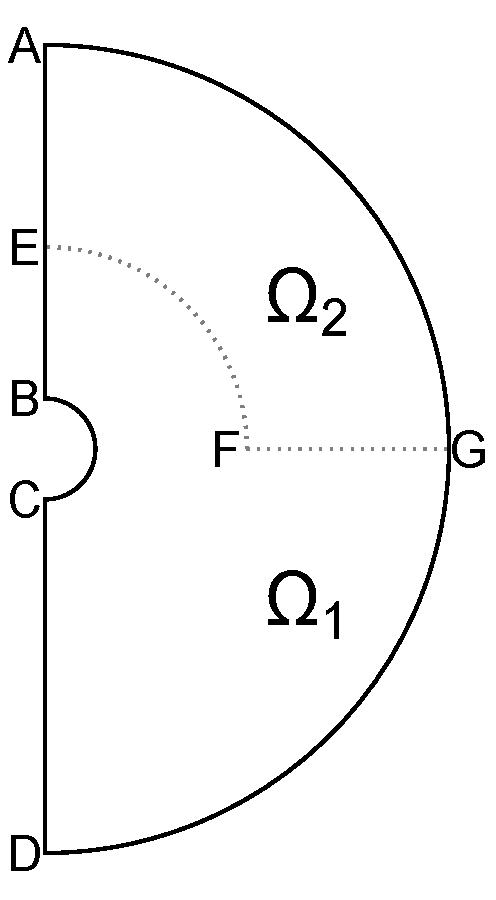
\includegraphics[scale=0.3]{images/ch4/section3_circular/domain.pdf}
    \caption{Область $\Omega$ представляет собой объединение 2 областей.}
    \label{fig:pt10:_domain}
\end{figure}


В области $\Omega = \Omega_1 \cup \Omega_2$ рассмотрим бильярдную систему, подчиняющуюся закону $(\ast)$.
В предыдущем разделе была введена функция $\Lambda(x,y,v_x, v_y)$: ее значение равно параметру $\alpha$ софокусной квадрики $\frac{x^2}{a^2-\alpha} + \frac{y^2}{b^2-\alpha} = 1$, которой касается бильярдная траектория, проходящая через точку $(x,y)$ с вектором скорости $(v_x, v_y)$.
% А именно, в области $\Omega_i$ значение $\Lambda(x,y,v_x, v_y) = \alpha_i$ является параметром квадрики, которая задается уравнением $\frac{x^2}{a^2-\alpha_i} + \frac{y^2}{b^2-\alpha_i} = 1$. 
В частном случае, когда большая и малая полуоси $a$ и $b$ эллипса  совпадают, уравнение квадрики можно записать в виде $x^2 + y^2 = a^2-\alpha = \rho^2$, где $\rho$ --- радиус окружности, касающейся звена траектории.
Величина $\rho^2$ является функцией положения и скорости материальной точки и задается формулой $$\rho^2(x,y,v_x,v_y) = a^2 - \Lambda(x, y, v_x, v_y) = \frac{(x v_y - y v_x)^2}{v_x^2 + v_y^2}.$$
Для классического бильярда в круге  функция $\rho^2$ является первым интегралом, не зависящим от полной энергии.

\section{Интеграл $\rho^2$. Условия полного внутреннего отражения}\label{sec:ch5/sec2}
Общая граница областей $\Omega_1$ и $\Omega_2$ состоит из двух кривых: из сегмента окружности $EF$ и отрезка прямой $FG$. 
Пусть материальная точка двигается с вектором скорости $(v_x, v_y)$ в области $\Omega_1$ и в точке с координатами $(x,y) \in EF \cup FG$ преломляется, после чего продолжает движение в области $\Omega_2$ с вектором скорости $(w_x, w_y)$. 

Проведем через точку $(x,y)$ прямую с вектором направления $(v_x, v_y)$: она касается некоторой окружности с центром в начале координат. Обозначим ее радиус через $\rho_1$. Аналогично $\rho_2$ определим как радиус окружности, касательной к проходящей через ту же точку $(x,y)$ прямой с вектором направления $(w_x, w_y)$.
Тогда в зависимости от того, к какой части общей границы областей $\Omega_1$ и $\Omega_2$  принадлежит точка $(x,y)$, величины $\rho_1^2$ и $\rho_2^2$ удовлетворяют одному из двух равенств. 
\begin{statement}
Имеют место следующие соотношения для параметров $\rho_1, \rho_2$ в точке преломления:
\begin{align}
(\rho_1^2 - r_1^2)n_1^2 = (\rho_2^2 - r_1^2)n_2^2 \qquad & 
			\text{ при } (x,y) \in EF, 
			\label{eq:st1_eq1}
			\\
\rho_1^2 n_1^2 = \rho_2^2 n_2^2 \qquad  & \text{ при } (x,y) \in FG.
			\label{eq:st1_eq2}
\end{align}
\label{st:across_EF}
\end{statement}
\begin{remark}
В доказательстве будут заодно отмечены условия, при которых бильярдная траектория преломляется и при которых испытывает полное  отражение.
\end{remark}

\begin{proof}
Пусть $(x,y) \in EF$, то есть траектория преломляется на дуге окружности с радиусом $r_1$. 
Угол $\theta_1$ откладывается между вектором скорости $(v_x, v_y)$ и вектором нормали окружности, который пропорционален радиус-вектору $(x,y)$. Тогда в обозначениях $\textbf{x}^2 = x^2+y^2$, $\textbf{v}^2=v_x^2+v_y^2$ рассмотрим величину
\begin{multline*}
\frac{r_1^2-\rho_1^2}{r_1^2} = \frac{1}{\textbf{x}^2} \left(\textbf{x}^2- \frac{(x v_y-y v_x)^2}{\textbf{v}^2}  \right) = \\
\frac{1}{\textbf{x}^2 \textbf{v}^2}\left( \textbf{x}^2 \textbf{v}^2 - (x^2 v_y^2 - 2xyv_xv_y+y^2v_x^2) \right) =
 \frac{1}{\textbf{x}^2\textbf{v}^2}\left( x^2 v_x^2 + 2xyv_xv_y+y^2v_y^2 \right) = \\
  \frac{1}{\textbf{x}^2\textbf{v}^2}(x v_x + y v_y)^2 = 
  \frac{1}{\textbf{x}^2\textbf{v}^2}\langle (x, y) , (v_x, v_y) \rangle^2 =
\cos^2 \theta_1,
\end{multline*}
где угол $\theta_1$ корректно определен при $\cos^2 \theta_1 \in (0,1)$, то есть косинус угла имеет смысл при $\rho_1^2 \in (0, r_1^2)$. 

Эта формула теряет смысл при $\rho_1 > r_1$ (когда бильярдная траектория не пересекает дугу $EF$) --- тогда $\cos^2 \theta_1 < 0$; случай $\cos^2 \theta_1 > 1$ соответствует $\rho_1^2 < 0$.
%Случай $\cos^2 \theta_1 <0$ соответствует $\rho_1 > r_1$, то есть дуга $EF$ и бильярдная траектория лежат по разные стороны от окружности радиуса $\rho_1$. 
%Неравенству $\cos^2 \theta_1 >1$ соответствует $\rho_1^2 <0$, что невозможно для вещественного радиуса $\rho_1$. 
Аналогичные соображения справедливы для $\cos^2 \theta_2 = \frac{r_1^2-\rho_2^2}{r_1^2}$.

Пусть $n_1 < n_2$. Тогда если величина $\frac{n_2}{n_1} \cos \theta_2 \in [-1,1]$, то в силу закона $(\ast)$ она совпадает с корректно определенным $\cos \theta_1$, откуда следует первое равенство утверждения. 
Остается лишь записать тождество  $(n_1 \cos \theta_1)^2 = (n_2 \cos \theta_2)^2$ через $r_1, \rho_1, \rho_2$, согласно приведенным выше выражениям.
При $\cos \theta_2 > \frac{n_1}{n_2}$ не существует удовлетворяющий закону преломления $\cos \theta_1$, и траектория отражается от $EF$ в область $\Omega_2$. 

Случай $n_1 > n_2$ рассматривается аналогично: величина $\frac{n_1}{n_2} \cos \theta_1 \in [-1,1]$, соответствует корректно определенному  $\cos \theta_2$, что позволяет получить нужное равенство. При $\cos \theta_1 > \frac{n_2}{n_1}$ траектория отражается от $EF$ в область $\Omega_1$. 


Пусть $(x,y) \in FG$, то есть траектория преломляется на отрезке горизонтальной прямой $\left\{ x \in (r_1,r_2), y=0 \right\}$. Тогда 
$$\frac{\rho_1^2}{x^2} = \frac{(x v_y-y v_x)^2}{x^2 \textbf{v}^2} = \frac{(x v_y)^2}{x^2 \textbf{v}^2} = \frac{v_y^2}{\textbf{v}^2} = \cos^2\theta_1, $$
аналогично получается равенство $\frac{\rho_2^2}{x^2} = \cos^2 \theta_2$. Из закона $(\ast)$ следует второе равенство утверждения везде, где корректно определены $\cos^2 \theta_1$ и $\cos^2 \theta_2$.
Опишем области корректного определения указанных величин.

Для первой координаты точки на сегменте $FG$ справедливо $x \in (r_1, r_2)$, следовательно $\frac{1}{x^2} \in (\frac{1}{r_2^2}, \frac{1}{r_1^2})$.
Косинус $\cos \theta_1$ корректно определен тогда и только тогда, когда $\frac{\rho_1^2}{x^2} \in (0,1)$, то есть $\frac{1}{x^2} \in (0,\frac{1}{\rho_1^2})$.
Комбинируя эти неравенства, выделим следующие случаи:

$\bullet$ При $\frac{1}{r_1^2} < \frac{1}{\rho_1^2}$ в каждой точке $FG$ определен $\cos \theta_1$;

$\bullet$ При $\frac{1}{r_2^2} < \frac{1}{\rho_1^2} < \frac{1}{r_1^2}$ в точках $x > \rho_1$ отрезка $FG$ определен $\cos \theta_1$;

$\bullet$ При $\frac{1}{\rho_1^2} < \frac{1}{r_2^2}$ ни в одной точке отрезка  $FG$ не определен $\cos \theta_1$.

Аналогично выделяются случаи, в которых определен $\cos \theta_2$. 
Таким образом, бильярдная траектория преломляется в любой точке $FG$ при $\max( \rho_1, \rho_2) < r_1$. При $r_1 < \max( \rho_1, \rho_2)$ траектория может преломиться в точках $(x,0) \in FG$, где $\max( \rho_1, \rho_2)  <x < r_2$. 

\end{proof}

\begin{remark}
Если траектория при переходе из $\Omega_1$ в $\Omega_2$ преломляется на дуге $EF$, то для величины $\rho_2^2$ справедливо $0 < \rho_2^2 < r_1^2$. 
И наоборот, если траектория при переходе из $\Omega_2$ в $\Omega_1$  преломляется на дуге $EF$, то для величины $\rho_1^2$ справедливо $0 < \rho_1^2 < r_1^2$. 
\label{cons:branching_zone_origins}
\end{remark}

Разобьем бильярдную траекторию в точках пересечения дуги $EF$ на фрагменты $T_k, k \geq 1$. 


%\textcolor{red}{=========== ниже плохое ===========}
% 
%Рассмотрим бильярдную траекторию, которая проходит из области $\Omega_1$ в область $\Omega_2$, пересекая отрезок $FG$, и возвращается в $\Omega_1$, пересекая дугу окружности $EF$. 
%Пусть радиус каустики до перехода через $FG$ равен $\rho_1$. 
%Из только что доказанного утверждения следует, что продолжения звеньев траектории после преломления на $FG$ касаются окружности радиуса $\rho_2$, где $\rho_2^2 = \rho_1^2 \frac{n_1^2}{n_2^2}$. 
%Если теперь траектория переходит через дугу $EF$, то после преломления звенья будут лежать на касательных прямых к окружности радиуса $\widetilde{\rho}_1 \neq \rho_1$, где $\widetilde{\rho}_1^2 = (\rho_2^2 - r_1^2)\frac{n_2^2}{n_1^2} + r_1^2$. 
%Подставим в полученное равенство выражение для $\rho_2^2$:
%\begin{equation}
%\widetilde{\rho}_1^2 = (\rho_2^2 - r_1^2)\frac{n_2^2}{n_1^2} + r_1^2 = \rho_1^2 +\frac{ r_1^2 (n_1^2 - n_2^2)}{n_1^2} = \rho_1^2 + \frac{\gamma}{n_1^2}, \ \gamma = r_1^2 (n_1^2-n_2^2),
%\label{eq:gammaDef}
%\end{equation}
%где коэффициент $\gamma$ не зависит от конкретного выбора траектории, которая проходит из области $\Omega_1$ в область $\Omega_2$, пересекая отрезок $FG$, и возвращается в $\Omega_1$, пересекая дугу окружности $EF$. 
%
%Предположим, что продолжение траектории <<обходит>> точку $F$ и снова пересекает отрезок $FG$. Тогда, повторяя вышеприведенные рассуждения для радиуса каустики $\widetilde{\rho}_2$ после второго преломления на отрезке $FG$, получим равенство $\widetilde{\rho}_2^2 = \rho_2^2 + \frac{\gamma}{n_2^2}$. 
%
%При обходе точки $F$ по часовой стрелке из параметров каустик $\rho_1^2$ и $\rho_2^2$ в областях $\Omega_1$ и $\Omega_2$ будут вычитаться  дроби $\frac{\gamma}{n_1^2}$ и $\frac{\gamma}{n_2^2}$, соответственно.
%
%Таким образом, на любой бильярдной траектории величина  $\rho_1^2$ в области $\Omega_1$ определена с точностью до добавления параметра $\frac{\gamma}{n_1^2}$, а $\rho_2^2$ в области $\Omega_2$ --- с точностью до добавления параметра $\frac{\gamma}{n_2^2}$. 
%
%\begin{remark}
%Обратим внимание на то, что на каждой траектории может появляться лишь конечное количество значений такого вида.
%
%Действительно, поскольку $\gamma$ (см. \eqref{eq:gammaDef}) не зависит от параметров траектории, то для произвольного $\rho_i < r_1$ начиная с некоторого $k$ выполняется $\rho_i + k \gamma > r_1$,  следовательно траектория не сможет пересечь дугу окружности $EF$. 
%
%Наоборот, для некоторого $m_0 > 0$ будет выполнено неравенство $\rho_i - m_0 \gamma < 0$. Тогда для всех $m\geq m_0$ выполнено $\rho_i - m \gamma  < 0$ и траектория отражается на ребре $EF$ или $FG$ в соответствии с законом $(\ast)$.
%\label{rem:finiteRevolutions}
%\end{remark}
%\textcolor{red}{=========== все ===========}

%Таким образом, в зависимости от того, по какому ребру траектория переходит из области $\Omega_1$ в область $\Omega_2$, радиус квадрики $\rho_2$ может быть определен одним из двух случаев. То есть, функция $\rho_2(\rho_1)$ является многозначной функцией. 

Каждый фрагмент бильярдной траектории $T_k$ образует ломаную кривую в $\Omega \setminus EF$, где $EF  \subset \partial \Omega_1 \cap \partial \Omega_2$.
Введем на $\Omega \setminus EF$ функцию $\Xi(x, y, v_x, v_y)$ по формуле
\begin{equation}
\Xi(x, y, v_x, v_y) = \left[
\begin{array}{ll}
    \rho^2(x,y,v_x,v_y) n_1^2, &  \text{ если } (x,y) \in \Omega_1 \\
    \rho^2(x,y,v_x,v_y) n_2^2, & \text{ если } (x,y) \in \Omega_2.
\end{array}
\right.
\label{eq:XiDefinition}
\end{equation}
Эта функция постоянна в каждой точке фрагмента бильярдной траектории $T_k$, но на разных фрагментах значения могут различаться. 

Рассмотрим значения интеграла $\Xi$ для двух последовательных фрагментов $T_k, T_{k+1}$. Выясним, как они связаны, или, что то же самое, как меняется интеграл $\Xi$ при преломлении на дуге $EF$. 

\begin{statement}
Значения $\Xi_k$ и $\Xi_{k+1}$  интеграла $\Xi$, соответствующие фрагментам траектории $T_k$ и $T_{k+1}$, различаются на величину $r_1^2(n_1^2-n_2^2)$.
\end{statement}
\begin{proof}
Значение $\Xi_k$ на фрагменте $T_k$ определяет радиусы $\rho_1$ и $\rho_2$ по формуле \eqref{eq:XiDefinition}. Здесь $\rho_1$ и $\rho_2$ являются радиусами окружностей, которых касаются звенья (или их продолжения) фрагмента $T_k$, содержащиеся в областях $\Omega_1$ и $\Omega_2$, соответственно.
Аналогично определяются радиусы $\widetilde{\rho}_1$ и $\widetilde{\rho}_2$ для фрагмента $T_{k+1}$ бильярдной траектории.
%касаются окружности радиуса $\rho_1$, а содержащиеся в $\Omega_2$ --- окружности радиуса $\rho_2$. Аналогично
%, которые определяют радиусы касательных окружностей к сегментам $T_k$


Пусть бильярдная траектория при преломлении на дуге $EF$ переходит из области $\Omega_1$ в область $\Omega_2$. 
%Обозначим радиус касательной к траектории окружности до преломления через $\rho_1$, а радиус аналогичной окружности после преломления в $\Omega_2$ --- через $\widetilde{\rho}_2$. 
Тогда радиусы $\rho_1^2$ и $\widetilde{\rho}_2^2$ связаны формулой \eqref{eq:st1_eq1}:  $(\rho_1^2 - r_1^2)n_1^2 = (\widetilde{\rho}_2^2 - r_1^2)n_2^2$.
С другой стороны, по формуле \eqref{eq:XiDefinition}: $\Xi_k = \rho_1^2 n_1^2$ и $\Xi_{k+1} = \widetilde{\rho}_2^2 n_2^2$.
Следовательно, $\Xi_k = \Xi_{k+1}  +r_1^2 (n_1^2 - n_2^2 )$.

Аналогично рассматривается случай, когда траектория переходит из области $\Omega_2$ в $\Omega_1$, преломляясь на дуге $EF$. Получим $\Xi_k = \Xi_{k+1}  - r_1^2 (n_1^2 - n_2^2 )$.
\end{proof}



%\textcolor{red}{=========== дальше может быть плохой текст ===========}
% 
%\textcolor{red}{Сюда картинку с ветвлением можно добавить.}
%В частности, в зависимости от отношения $\frac{n_1}{n_2}$ интеграл $\Xi$ растет при пересечении дуги $EF$ в направлении по или против часовой стрелки.

% принимает одно и то же значение в каждой точке на любых отрезках траекторий, не пересекающих дугу $EF$. Переход из $\Omega_2$ в область $\Omega_1$ через эту дугу увеличивает значение $\Xi$ на $\gamma$, а переход в обратном направлении --- уменьшает на $\gamma$.
%При этом $\Xi(x,y,v_x,v_y) \mod \gamma$ принимает одно и то же значение для всех звеньев любой траектории. Обратим внимание, что если рассматривать $\Xi$ как многозначную функцию со значениями в $\mathbb{R}$, то на каждой траектории функция $\Xi$ принимает лишь конечное количество значений.
%
%Задача состоит в том, чтобы для указанной динамической системы описать слоение изоэнергетического трехмерного многообразия на поверхности уровня первого интеграла $\Xi$. 

\medskip
Значению интеграла $\Xi$ поставим в соответствие точку плоскости $\mathbb{R}^2$ по формуле 
\begin{equation}
\Xi \mapsto P(\Xi) = (\rho_1^2, \rho_2^2) = \left( \frac{\Xi}{n_1^2}, \frac{\Xi}{n_2^2} \right).
% = \left( \left. \rho^2 \right|_{\Omega_1} ,  \left. \rho^2 \right|_{\Omega_2}  \right).
\label{eq:XiMap}
\end{equation}
Если рассмотреть фрагмент $T_k$ бильярдной траектории, который проходит по обеим областям $\Omega_1$ и $\Omega_2$, то первая (вторая) координата точки $P(\Xi_k)$ является квадратом радиуса окружности $\rho_1$($\rho_2$), которой касаются звенья фрагмента $T_k$, лежащие в $\Omega_1$ (в $\Omega_2$). 
Отметим, что если фрагмент $T_k$ целиком содержится в $\Omega_1$ (в $\Omega_2$), то только первая (вторая) координата точки $P(\Xi_k)$ имеет смысл, а другая координата информации не несет.
\medskip
\begin{remark}
Для фиксированных $r_1, n_1, n_2$ точка $P(\Xi_k)$, соответствующая каждому фрагменту бильярдной траектории $T_k$, лежит на прямой $L$, которая в декартовых координатах $(\rho_1^2, \rho_2^2)$ задается уравнением 
\begin{equation}
\rho_2^2 = \rho_1^2 \frac{n_1^2}{n_2^2}.
\label{eq:lineL}
\end{equation}

\end{remark}

%При пересечении линии разреза $EF$ величина $\Xi$ испытывает скачок на постоянную $\gamma$, которая не зависит от параметров каустик. После преломления на дуге $EF$ точка 
%\begin{equation}
%\rho^2(\Xi \pm \gamma) = (\widetilde{\rho}_1^2,\widetilde{\rho}_2^2) = (\rho_1^2 \pm \frac{\gamma}{n_1^2}, \rho_2^2 \pm \frac{\gamma}{n_2^2})
%\label{eq:shiftedXi}
%\end{equation}
% остается на прямой  \eqref{eq:lineL}.
%, поскольку 
%$$\widetilde{\rho}_2^2 = \rho_2^2 \pm \frac{\gamma}{n_2^2} = \rho_1^2 \frac{n_1^2}{n_2^2} \pm \frac{\gamma}{n_2^2} = \widetilde{\rho}_1^2 \frac{n_1^2}{n_2^2}$$
%удовлетворяет тому же уравнению прямой

Наглядно можно представлять себе, что возможные случаи соотношений между числами $r_1, n_1, n_2$ соответствуют всевозможным прямым, проходящим через начало координат и образующим   с горизонтальной осью угол $\theta = \arctg \frac{n_1^2}{n_2^2}$, который меняется от $0$ до $\frac{\pi}{2}$.

%\marginpar{тут остановились}
Дальнейший анализ задачи Б по сравнению с задачей А значительно сложнее из-за того, что $\Xi$ может испытывать скачки.
Но вместе с тем ясно, что при анализе системы нужно следить за тем, как по отношению к величинам $r_0^2, r_1^2, r_2^2$ расположены значения $\dfrac{\Xi}{n_1^2}$ и $\dfrac{\Xi}{n_2^2}$, то есть квадраты радиусов окружностей, касающихся звеньев траектории, расположенных в областях $\Omega_1$ и $\Omega_2$, соответственно.
\begin{remark}
Ясно, что на форму траектории влияют не абсолютные величины $n_1, n_2$, а только их отношение. Поэтому в дальнейшем мы будем предполагать их нормированными таким образом, что $\dfrac{1}{n_1^4} + \dfrac{1}{n_2^4} = 1$.
Удобно выбрать угол $0 < \theta < \frac{\pi}{2}$, для которого $\tg{\theta} = \dfrac{n_1^2}{n_2^2}$.
\end{remark}

Отображение $\Xi \mapsto P(\Xi)$, заданное формулой \eqref{eq:XiMap}, запишем в виде 
$$P(\Xi) = \left( \Xi \cos \theta, \Xi \sin \theta \right).$$
%Вектор сдвига (см. \eqref{eq:shiftedXi}), соответствующий скачку $\Xi$ на $\gamma$ при переходе через дугу $EF$, выражается как $\gamma_L = (\frac{\gamma}{n_1^2}, \frac{\gamma}{n_2^2}) = (\gamma \cos \theta, \gamma\sin\theta)$.

\begin{remark}
Для произвольной точки плоскости с координатами $(\rho_1^2, \rho_2^2)$ соответствующая ей прямая $L$ определяется углом $\theta = \arctg \frac{\rho_2^2}{\rho_1^2}$. Соответствующее точке значение $\Xi$ на этой прямой $L$ совпадает с нормой радиус-вектора точки.
Для величины $\gamma = r_1^2 (n_1^2 - n_2^2)$ между значениями $\Xi_k$ и $\Xi_{k+1}$  справедливо следующее выражение:
$$\gamma = r_1^2 (n_1^2 - n_2^2) = r_1^2 \left( \frac{1}{\cos \theta} -  \frac{1}{\sin \theta} \right).$$

\end{remark}

Параметризуем прямую $L$: $\xi \mapsto P(\xi) = (\xi \cos \theta, \xi \sin \theta)$.
Прямая $L$, заданная уравнением \eqref{eq:lineL} пересекает координатную линию $\{ \rho_1^2 = r_1^2 \}$ в точке $(r_1^2, r_1^2 \tg \theta) = P(\frac{r_1^2}{\cos \theta})$.
Аналогично, прямая $L$ и координатная линия $\{ \rho_2^2 = r_1^2 \}$ пересекаются в точке $(\frac{r_1^2}{\tg \theta}, r_1^2) = P(\frac{r_1^2}{\sin \theta})$. 

\begin{remark}
Удобно выбрать $\gamma$ положительным. Для $n_1^2 < n_2^2$ имеем $\theta < \frac{\pi}{4}$ и тогда $\frac{1}{\sin \theta} - \frac{1}{\cos \theta} > 0$, поэтому положим $\gamma =  r_1^2 \left( \frac{1}{\sin \theta} - \frac{1}{\cos \theta}  \right)$. В случае $n_1^2 > n_2^2$ величину $\gamma$ определим как $\gamma =  r_1^2 \left( \frac{1}{\cos \theta} - \frac{1}{\sin \theta}  \right)$.
Также определим точки пересечения $L$ с координатными линиями $\{ \rho_1^2 = r_1^2 \}$ и $\{ \rho_2^2 = r_1^2 \}$  как $L_0 = P(\frac{r_1^2}{\cos \theta})$ и  $L_1 = P(\frac{r_1^2}{\sin \theta})$ для $n_1^2 < n_2^2$ и наоборот, если $n_1^2>n_2^2$. 
Тогда вне зависимости от отношения $n_1^2 : n_2^2$ выполняются соотношения  $\gamma_L =  \overrightarrow{L_0 L_1}$ и $\gamma > 0$.
Здесь вектор $\gamma_L$ соответствует вектору, направленному из точки $P(\Xi_k)$ в точку $P(\Xi_{k+1})$, где $\Xi_k < \Xi_{k+1}$.
\label{rem:L0_L1_def}
\end{remark}

В определениях замечания \ref{rem:L0_L1_def} направления роста и убывания интеграла $\Xi$ можно проиллюстрировать на примере рис. \ref{fig:n1gtn2_Xi_growth} и \ref{fig:n1ltn2_Xi_growth}.
\begin{figure}[!htb]
\minipage{0.5\textwidth}
\centering
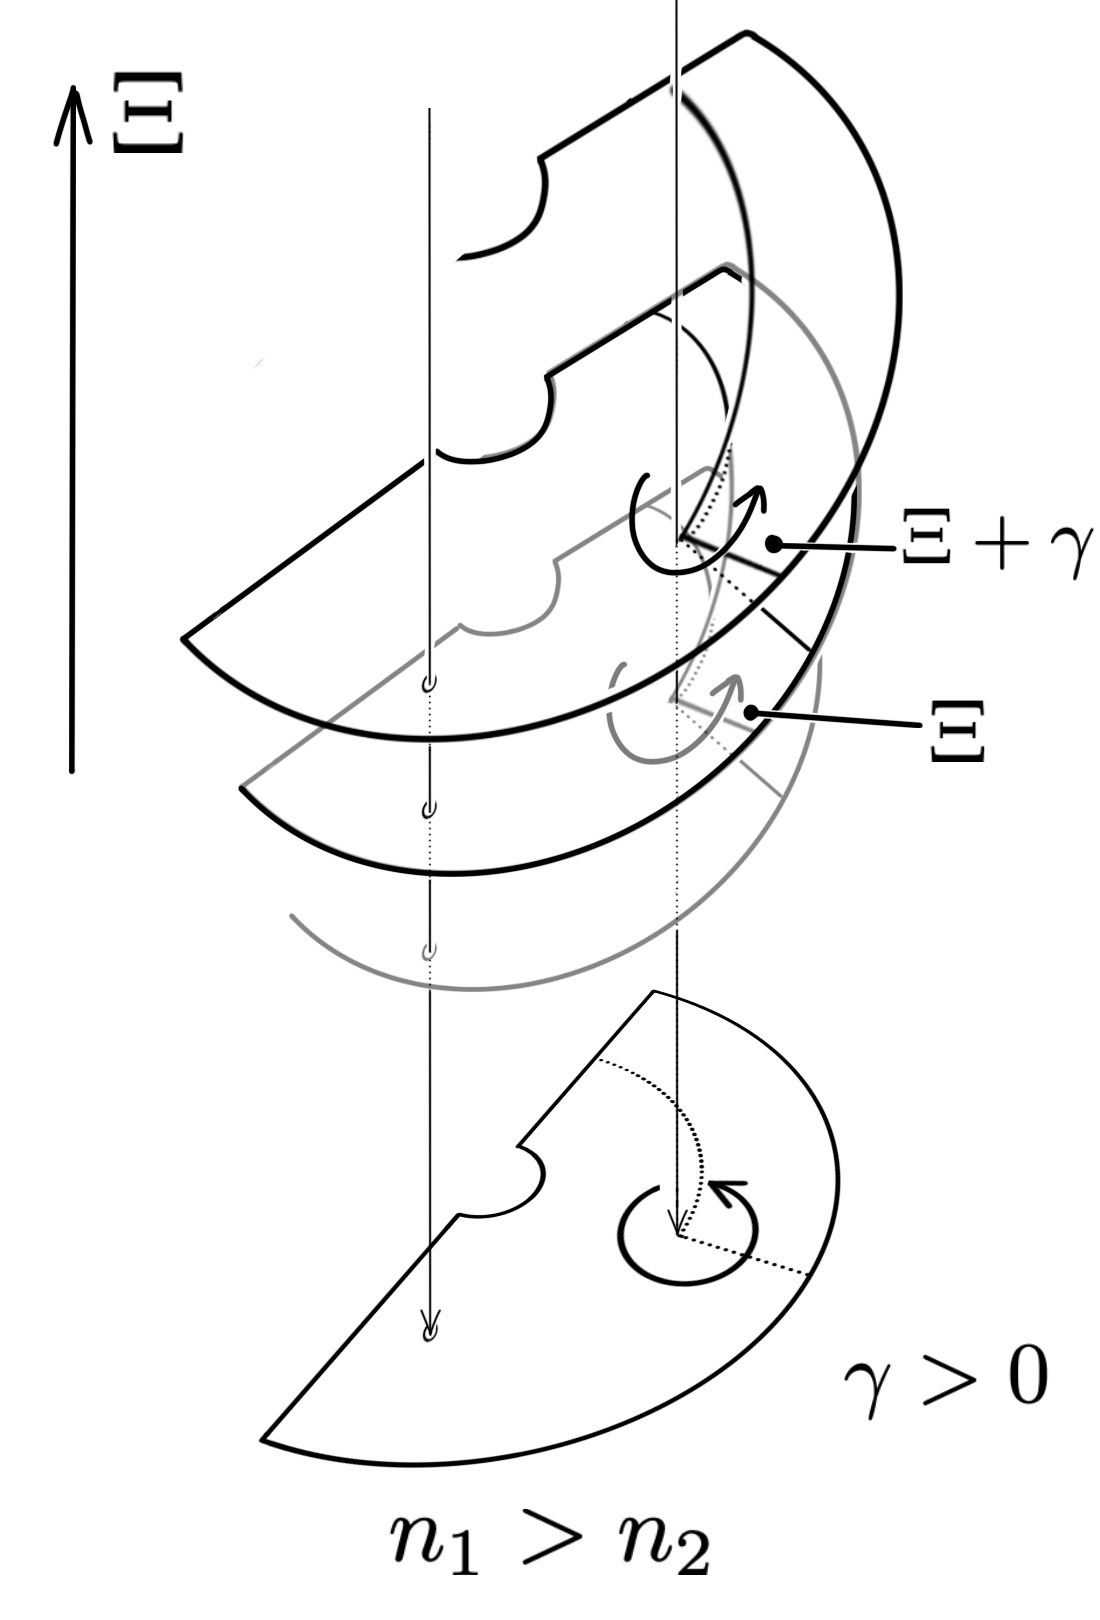
\includegraphics[width=5cm]{images/ch4/section3_circular/n1gtn2.png}
    \caption{Направление роста $\Xi$ при $n_1 > n_2$.}
    \label{fig:n1gtn2_Xi_growth}
\endminipage\hfill
\minipage{0.5\textwidth}
\centering
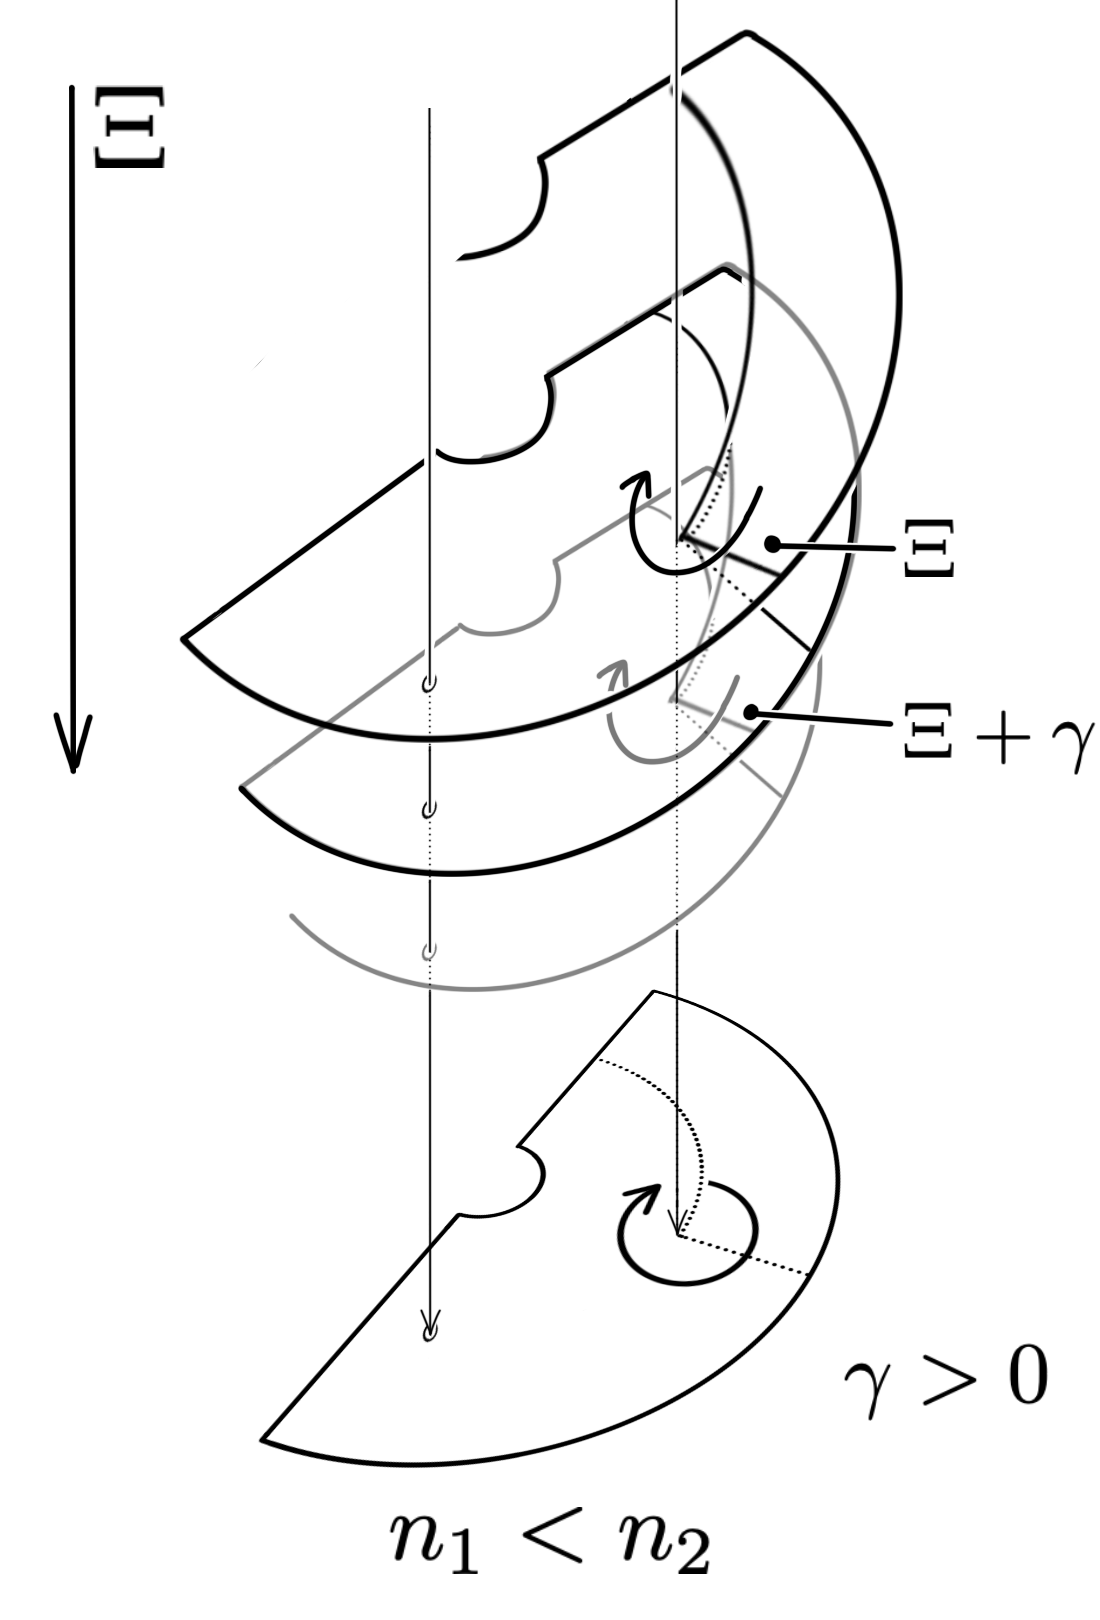
\includegraphics[width=5cm]{images/ch4/section3_circular/n1ltn2.png}
    \caption{Направление роста $\Xi$ при $n_1 < n_2$.}
    \label{fig:n1ltn2_Xi_growth}
\endminipage\hfill
\end{figure}

\medskip

%Тогда 
%$$\gamma_L = r_1^2 \left( \frac{1}{\sin \theta} - \frac{1}{\cos \theta}  \right) = L_1-L_0. $$
Точка $L_1$ разделяет прямую $L$ на две части относительно параметра $\xi$ на прямой $L$: $\left\{\xi < L_1\right\}$ и $\left\{\xi > L_1\right\}$. 
Объединяя эти части по всевозможным прямым $L$, получим области в $\mathbb{R}^2$, изображенные на  рис. \ref{fig:pt10:_lineDomains_simple}. Формальные определения областей см. неравенства \eqref{eq:xiLeqL1_strict} и \eqref{eq:xiGeqL1_strict}.

При этом в силу замечания \ref{cons:branching_zone_origins} если бильярдная траектория пересекает $EF$ хотя бы однажды, тогда точки, соответствующие фрагментам $T_k$ такой траектории, находятся только на части прямой $L$, попадающей внутрь области $\{ \xi < L_1\}$, изображенной на рис. \ref{fig:pt10:_lineDomains_simple}.

\begin{figure}[!htb]
    \begin{minipage}[c]{0.4\textwidth}
\centering
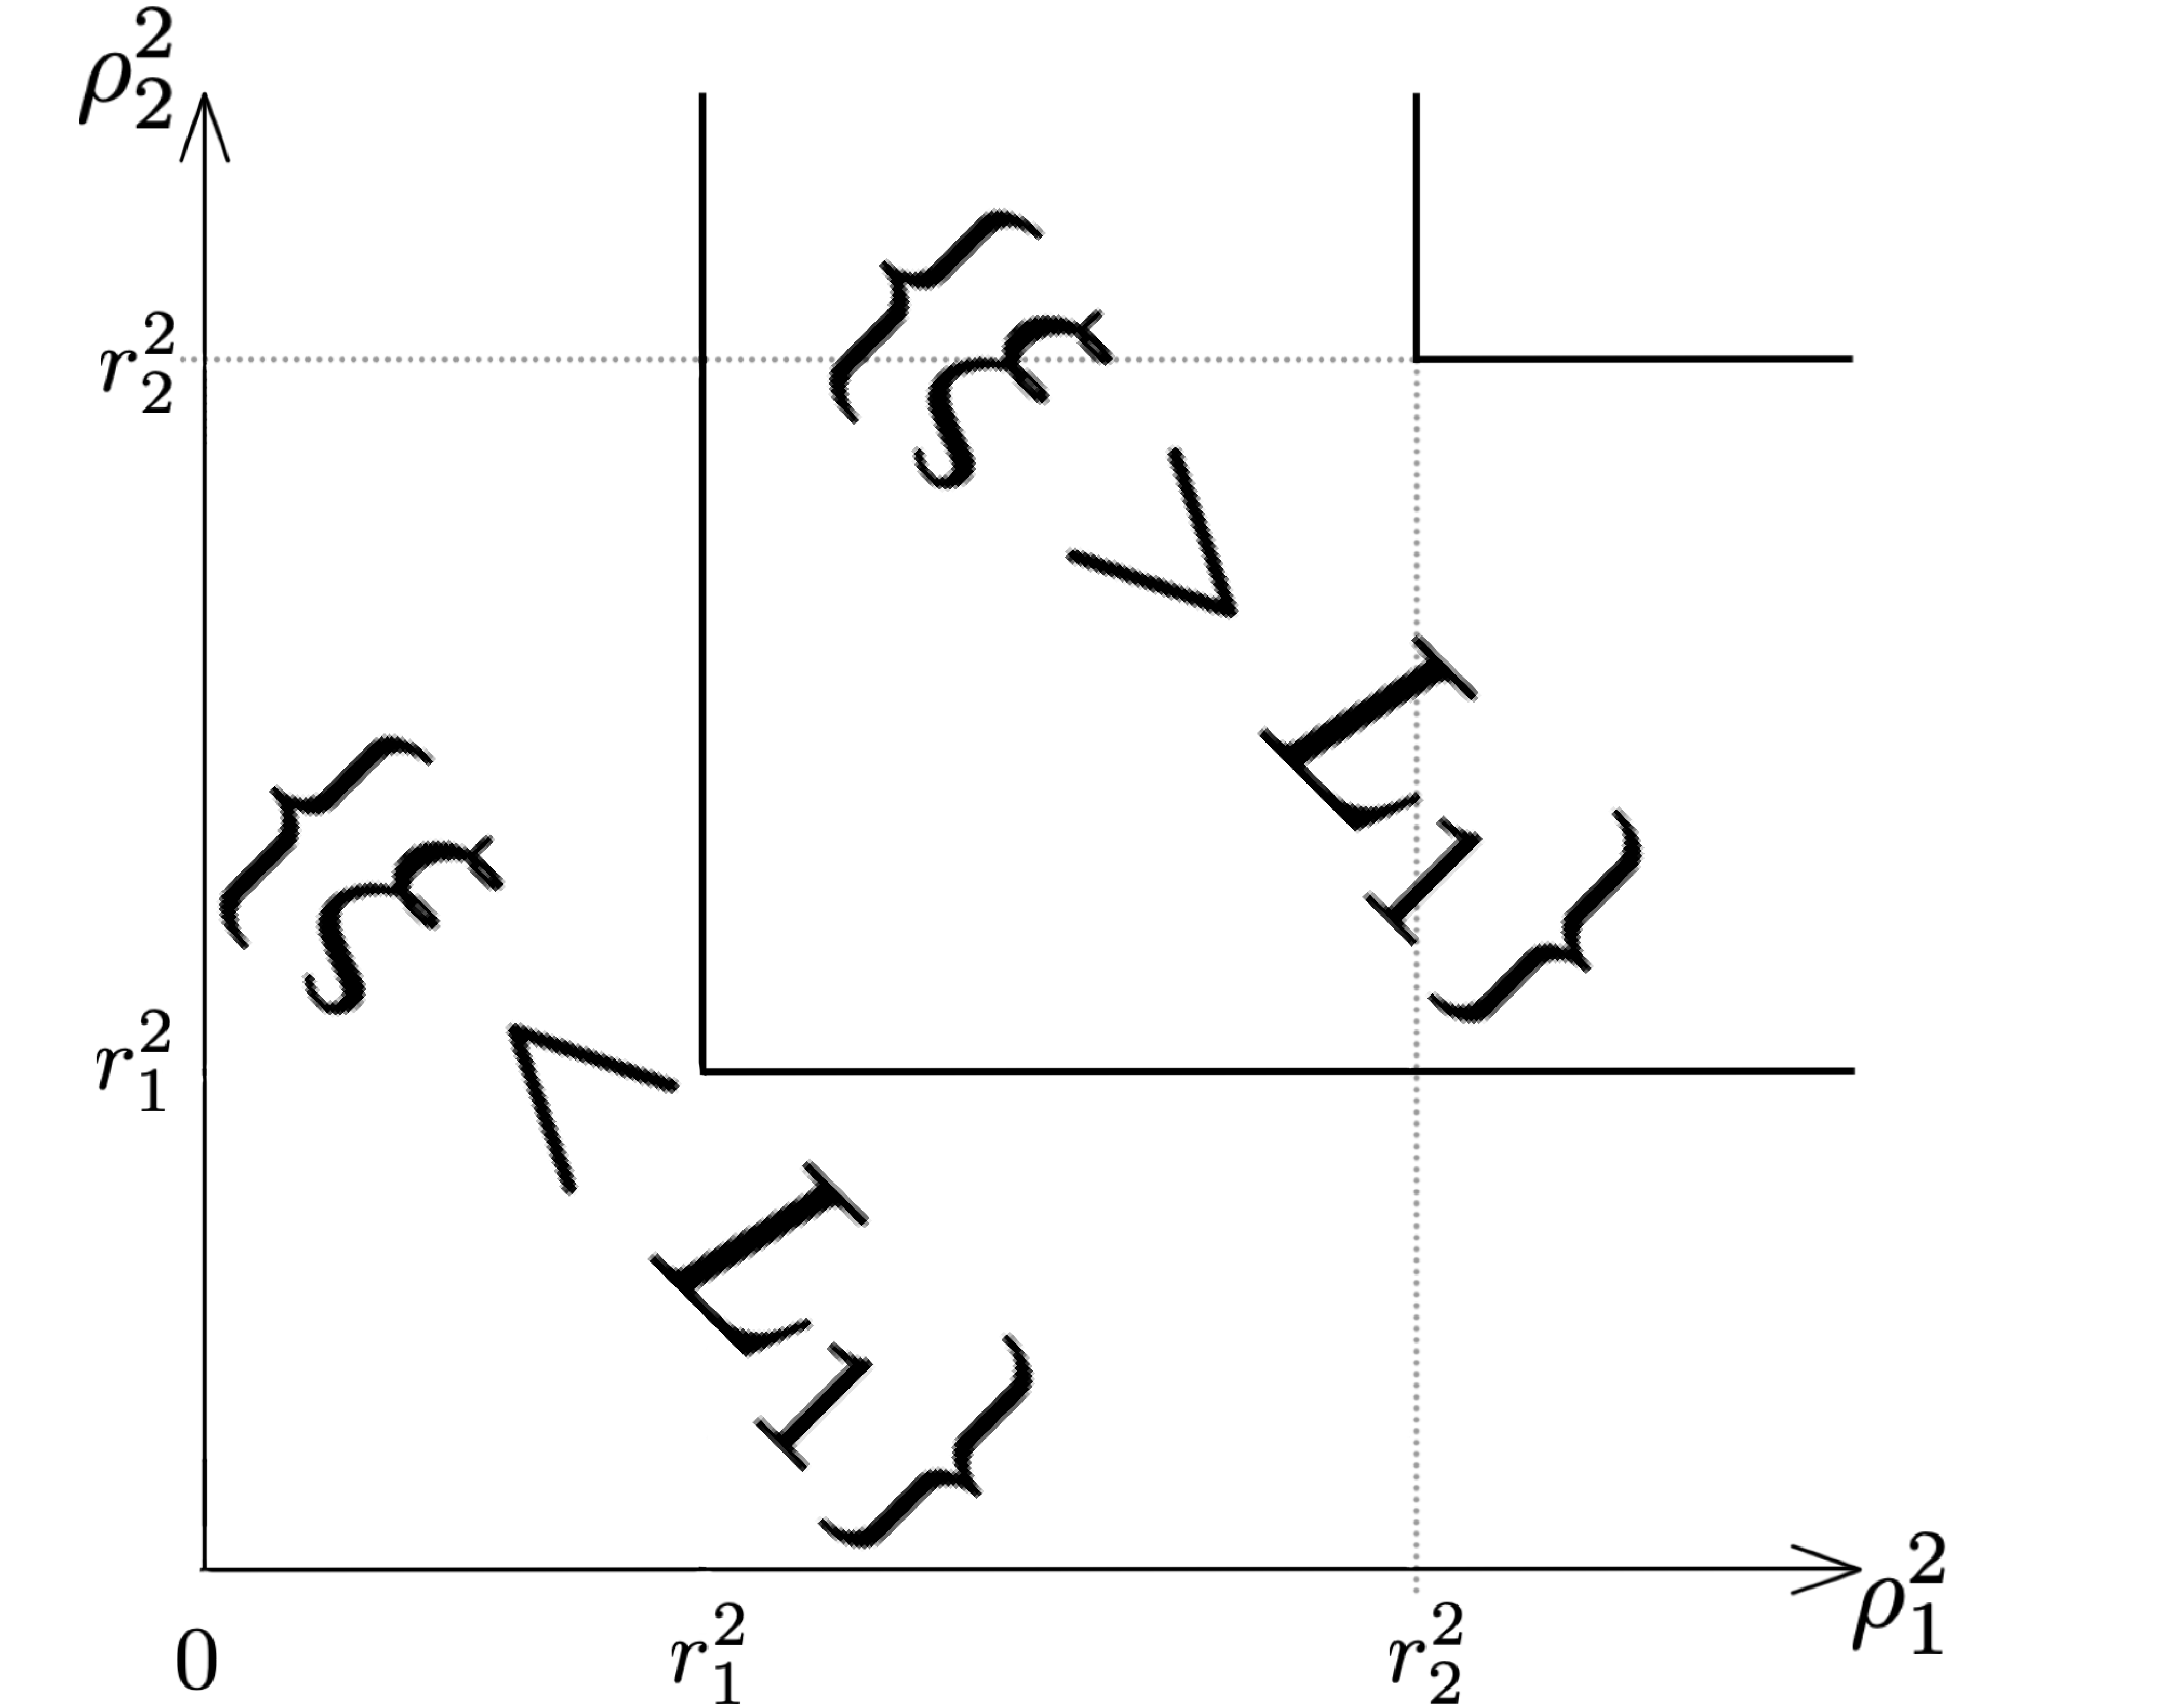
\includegraphics[scale=0.07]{images/ch4/section3_circular/line_domains_simple.pdf}
    \caption{Области $\left\{\xi< L_1\right\}$ и $\left\{\xi > L_1\right\}$.}
    \label{fig:pt10:_lineDomains_simple}
     \end{minipage}
     \begin{minipage}{0.6\textwidth}
\begin{align}
\left\{\xi < L_1 \right\} &=  \left\{\rho_1^2 > 0 , \rho_2^2 > 0 \right\} \setminus \left\{\rho_1^2 > r_1^2 , \rho_2^2 > r_1^2  \right\}, 
\label{eq:xiLeqL1_strict}
\\[15pt]
\left\{\xi > L_1\right\} &= \left\{\rho_1^2 > r_1^2 , \rho_2^2 > r_1^2\right\} \setminus \left\{\rho_1^2 > r_2^2 , \rho_2^2 > r_2^2  \right\}.
\label{eq:xiGeqL1_strict}
\end{align}

    \end{minipage}
\end{figure}

%Приведем соображения, специфичные для случая $\left\{\xi < L_1\right\}$. 

\section{Случай $\left\{\xi < L_1\right\}$}\label{sec:ch5/sec3}

В область $\{ \xi < L_1\}$ попадают точки, соответствующие таким и только таким фрагментам бильярдных траекторий, которые хотя бы в одной точке попадают на дугу $EF$. 
При этом любым двум соседним фрагментам $T_m, T_{m+1}$ таких траекторий на прямой $L$ соответствуют такие точки $P(\Xi_m), P(\Xi_{m+1}) = P(\Xi_m \pm \gamma)$, которые соединяются вектором $\gamma_L$.

В силу коллинеарности радиус-векторов точек $L_0$ и $L_1$,  справедливо равенство 
$$\gamma = ||\gamma_L|| = ||L_1-L_0|| = ||L_1||-||L_0|| < ||L_1||.$$
Введем величину 
\begin{equation}
\varepsilon = ||L_1||  - k \gamma, \text{ где } k=\left \lfloor \frac{||L_1||}{\gamma} \right \rfloor.
\label{eq:kDef}
\end{equation}
Тогда для $\xi < \varepsilon$ справедливо следующее неравенство:
$$\xi + k \gamma < \varepsilon + k \gamma =
 \varepsilon + \left \lfloor \frac{||L_1||}{\gamma} \right \rfloor \gamma = ||L_1||.$$
Для $\varepsilon< \xi <\gamma$ получим
\[
\begin{array}{cc}
\xi + (k-1) \gamma  < \gamma + (k-1) \gamma < ||L_1||, \\
\xi + k \gamma  > \varepsilon + k \gamma =  ||L_1||.
\end{array}
\] 
Рассмотрим произвольную пару параметров $r_1, n_1/n_2$ и прямую $L$, соответствующую ей. Положим $k=\left \lfloor \frac{||L_1||}{\gamma} \right \rfloor$. Тогда множество точек вида $(\rho_1^2, \rho_2^2) = P(\xi) \in [0, L_1] \subset L$, можно разделить на два непересекающихся множества:
\begin{equation*}
\begin{array}{ll}
    \widetilde{C}_{k+1}, & \text{ если } \left\{\dfrac{\xi}{\gamma}\right\} < \dfrac{\varepsilon}{\gamma}, \\
    \widetilde{C}_k, & \text{ если } \left\{\dfrac{\xi}{\gamma}\right\} > \dfrac{\varepsilon}{\gamma}.
\end{array}
\end{equation*} 
Теперь заметим, что $\Xi_m = \Xi_1 \mod \gamma$,
т.е. $\Xi_m$ отличается от $\Xi_1$ на целочисленное кратное $\gamma$. Однако набор всех значений $\Xi_m$ на траектории конечен. Это легко видеть из рис.     \ref{fig:pt10:_lineDomains_simple}. А именно, точки $P(\Xi)$ должны лежать на отрезке, соединяющем точку $0$ и точку $L_1$.

Отсюда следует, что если на каком-то  фрагменте $T_{m_0}$ бильярдной траектории  значение $\Xi_{m_0}$ принадлежит $\widetilde{C}_n$, тогда множество значений $\Xi_m$ для всех фрагментов $T_m$ этой же бильярдной траектории содержится в $\widetilde{C}_n$.

Таким образом, мы доказали следующее утверждение:
\begin{statement}
Если на  бильярдной траектории для какого-то ее фрагмента $T_{m_0}$  выполнено $\Xi_{m_0} \in \widetilde{C}_n, \ n\geq 1$, то на этой бильярдной траектории  $\Xi$ принимает не более $n$ различных значений. Значение $\Xi$ меняется при пересечении траекторией дуги $EF$.
\end{statement}

\begin{statement}
Для величины $k$, заданной соотношением $\eqref{eq:kDef}$, справедлива формула 
\[
k=\left\{
\begin{array}{ll}
\left\lfloor \dfrac{n_2^2}{n_2^2-n_1^2} \right\rfloor & n_1<n_2; \\
\\
\left\lfloor \dfrac{n_1^2}{n_1^2-n_2^2} \right\rfloor & n_1>n_2.
\end{array}
\right.
\]
%\frac{1}{1-\tg \theta}$, где $\tg \theta = \frac{n_1^2}{n_2^2}$. 
\end{statement}
\begin{proof}
Согласно замечанию \ref{rem:L0_L1_def}, для $n_1<n_2$ справедливы определения $L_1 = P(\frac{r_1^2}{\sin \theta})$ и $\gamma = r_1^2 \left( \frac{1}{\sin \theta} - \frac{1}{\cos \theta}  \right)$.
Тогда 
$$\frac{||L_1||}{\gamma} = \frac{r_1^2}{\sin \theta} \frac{\sin \theta \cos \theta}{r_1^2 (\cos \theta - \sin \theta)} = \frac{1}{1-\tg \theta},$$
где из равенства $\tg \theta = \frac{n_1^2}{n_2^2}$ получим $\frac{||L_1||}{\gamma} = \frac{n_2^2}{n_2^2-n_1^2}$. Целая часть от левой части равенства совпадает с $k$.

Для $n_1>n_2$ нужно рассуждать аналогичным образом, с учетом того, что в этом случае $L_1 = P(\frac{r_1^2}{\cos \theta})$ и $\gamma = r_1^2 \left( \frac{1}{\cos \theta} - \frac{1}{\sin \theta}  \right)$ (см. зам. \ref{rem:L0_L1_def}).
\end{proof}

Объединим множества $\widetilde{C}_k$ по всевозможным прямым $L$ \eqref{eq:lineL}, определенным всевозможными отношениями $\frac{n_1^2}{n_2^2}$. Аналогичным образом объединим $\widetilde{C}_{k+1}$ по всевозможным прямым $L$. Эти объединения будем обозначать $C_k$ и $C_{k+1}$, соответственно.

Опишем кривые, которые разделяют множества $C_k$ и $C_{k+1}$. 
Если $(x,y)$ --- точка плоскости, то положим $||(x,y)|| = \sqrt{x^2+y^2}$ --- расстояние до начала координат. В рассуждениях ниже $\xi = ||(\rho_1^2, \rho_2^2)||$. Введем обозначения для трех семейств кривых:
\begin{equation}
I = \{ ||L_1|| = m \gamma \}_{m \geq 2}, \ II = \{ \xi = m \gamma\}_{m \geq 1}, \ III = \{ \xi = m \gamma + \varepsilon\}_{m \geq 0}.
\label{eq:families_def}
\end{equation}
%\textcolor{red}{???????????????????? Ниже все плохо}
%
%
%
%
%Мы введем структурную диаграмму критических значений первого интеграла $\Xi$, см. рис. \ref{fig:pt10:_lineDomains}.
%\begin{figure}[!htb]
%%\minipage{0.45\textwidth}
%\centering
%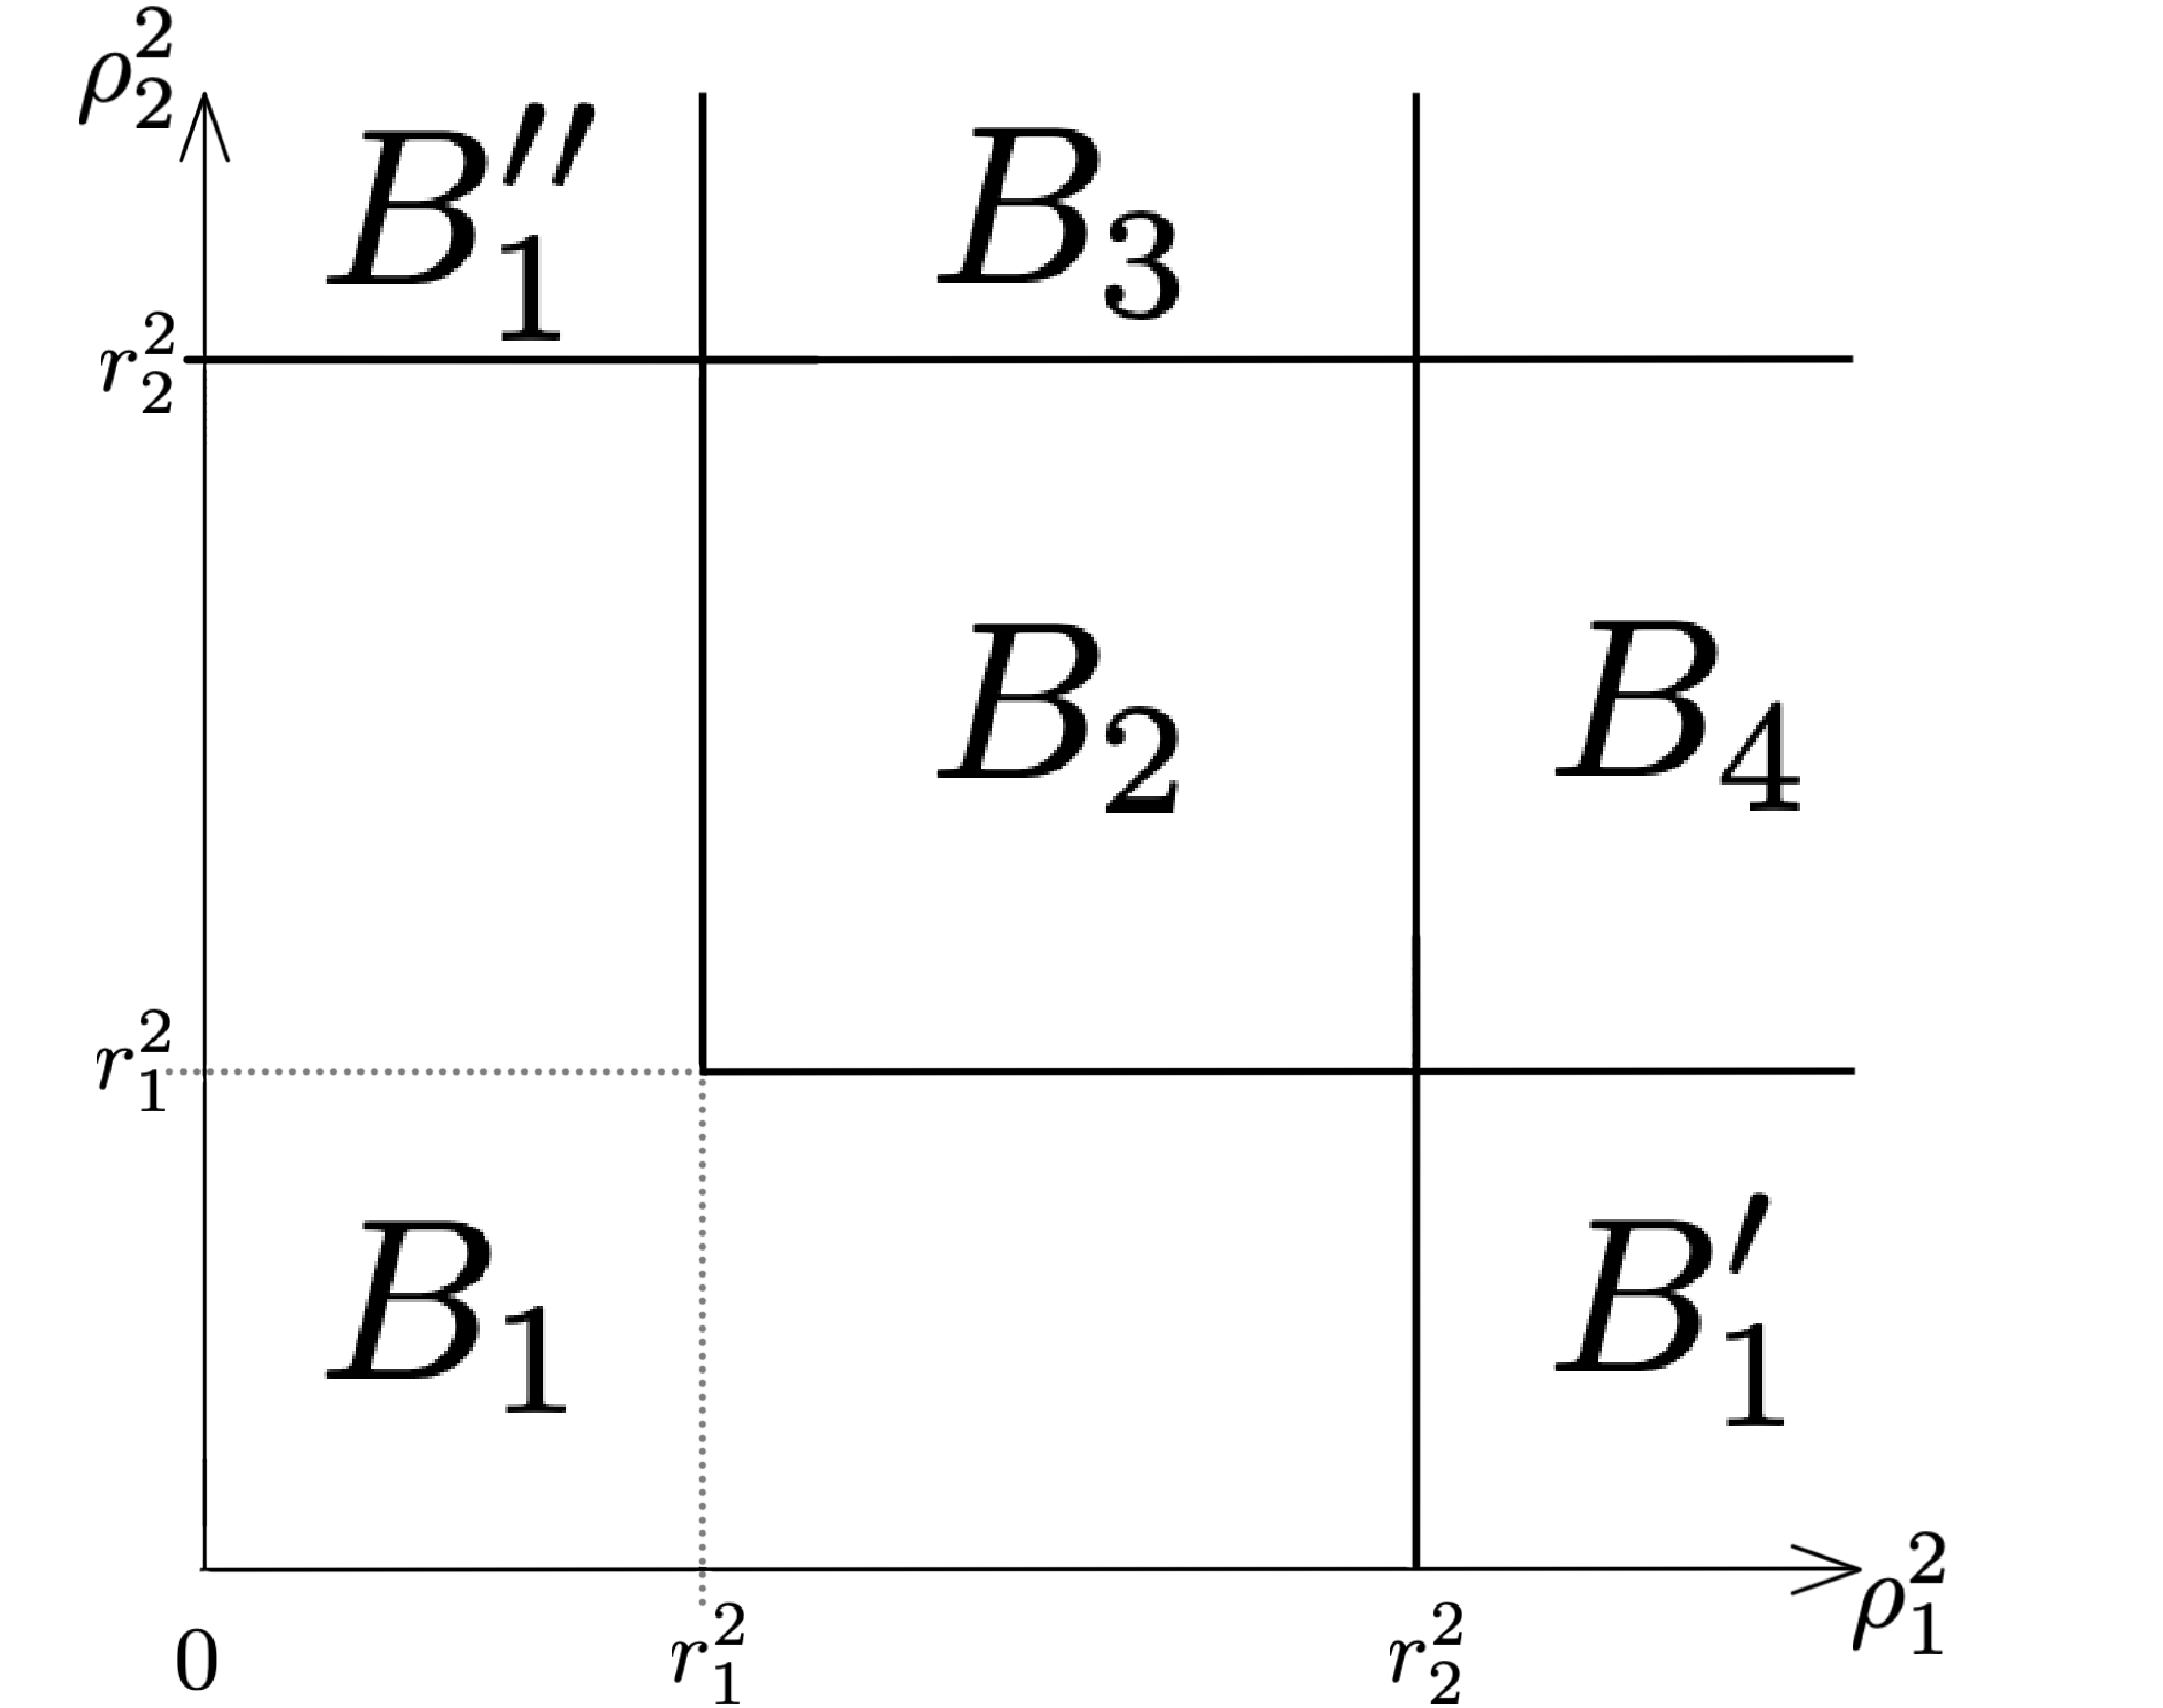
\includegraphics[scale=0.1]{images/ch4/section3_circular/line_domains.pdf}
%    \caption{Области возможного движения бильярдной траектории.}
%    \label{fig:pt10:_lineDomains}
%%\endminipage\hfill
%%\minipage{0.45\textwidth}
%%\centering
%%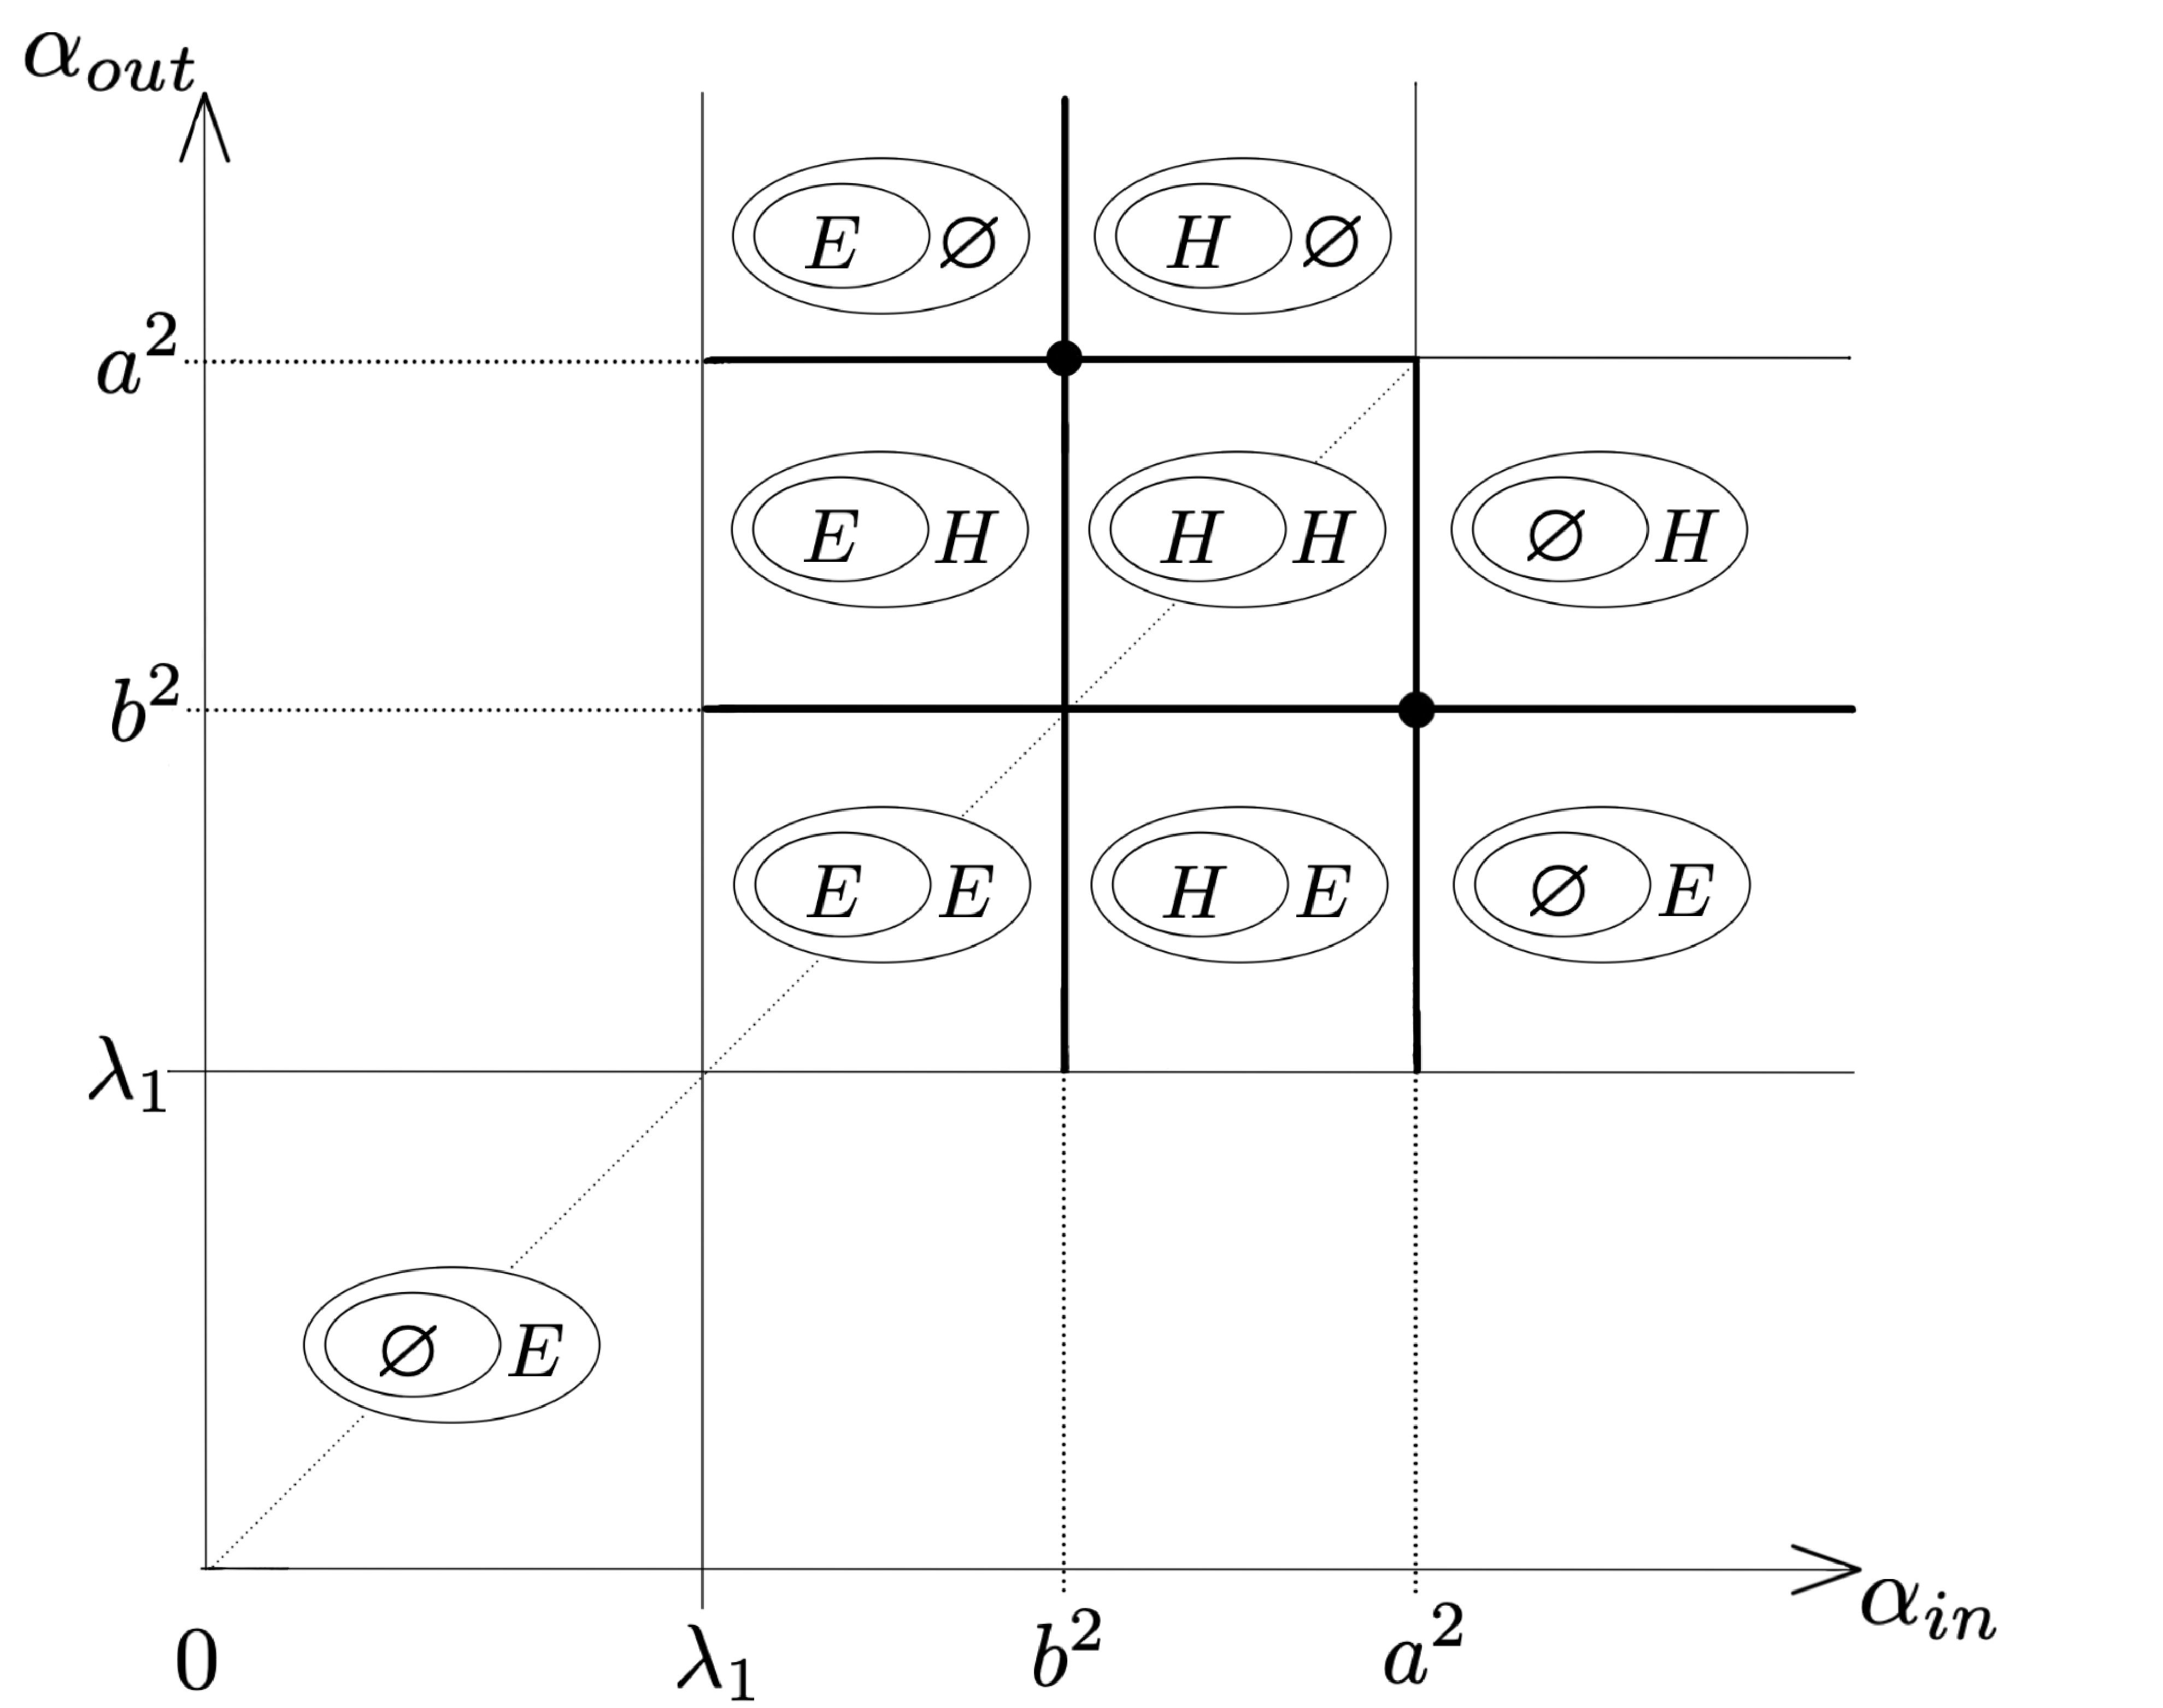
\includegraphics[scale=0.1]{images/ch4/section3_circular/problemAbifurcations.pdf}
%%    \caption{Возможные типы каустик в $\Omega_{in}$ и $\Omega_{out}$. Жирным выделены особые значения для $\alpha_{in}$, $\alpha_{out}$. См. также замечание \ref{rem:remark1}}
%%    \label{fig:pt10:_problemAbifurcations}
%%\endminipage\hfill
%\end{figure}
%
%$B_1, B_1', B_1'':$ Сначала рассмотрим траектории, которые выходят на оба сегмента $EF$ и $FG$ общей границы областей $\partial \Omega_1 \cap \partial \Omega_2$. Будем обозначать через $\rho_1$ и $\rho_2$ радиусы окружностей, которых касаются отрезки траектории бильярда, находящиеся в областях $\Omega_1$ и $\Omega_2$, соответственно.
%
%$B_2:$ Для достаточно больших $\rho_i$ дуга $EF$ попадает во внутренность каустических окружностей, в результате траектория перемещается между $\Omega_1$ и $\Omega_2$, пересекая только сегмент их общей границы $FG$.
%
%$B_3:$ В случае, если траектория целиком содержится в $\Omega_1$, параметр $\rho_2$ не определен. Такие траектории испытывают полное внутреннее отражение на ребрах $EF$ и $FG$. 
%
%$B_4:$ Аналогично для траекторий, целиком содержащихся в $\Omega_2$, параметр $\rho_1$ также не определен. Такие траектории испытывают полное внутреннее отражение на ребрах $EF$ и $FG$. 
%
%Анализ слоения на поверхности уровня интеграла $\Xi$ проходит по следующей схеме. Сначала фиксируются параметры $r_1, n_1, n_2$. Они определяют прямую $L$, при этом значение интеграла $\Xi$ однозначно определяет точку на этой прямой. Структура слоения определяется тем, как прямая $L$ пересекает области $B_1,\ldots, B_4, B_1', B_1''$.
%
%\begin{remark} В случае, когда совпадают коэффициенты $n_1, n_2$, траектории проходят из $\Omega_1$ в $\Omega_2$ и обратно без преломления, тем самым мы получаем динамику классического бильярда в половине диска. Этому  соответствует прямая $L$, проходящая по диагонали на рис. \ref{fig:pt10:_lineDomains}.
%\end{remark}
%
%\begin{remark}
%Здесь и далее $n_1$ и $n_2$ нас интересуют только с точностью до пропорциональности.
%\end{remark}
%
%\section{Соображения для случая $B_1$}\label{s3.4}
%\begin{remark}
%Здесь мы сознательно игнорируем случаи $B_1'$ и $B_1''$ для простоты. Эти случаи будут разобраны ниже после знакомства читателя с полезной диаграммой.
%\end{remark}
%Рассмотрим подробно особенности движения случая $B_1$.
%Из уравнения прямой $L$ \eqref{eq:lineL} положим $\theta = \arctg \frac{n_1^2}{n_2^2}$, тогда отображение $\Xi \mapsto \rho^2(\Xi)$ \eqref{eq:XiMap} можно записать в виде 
%$$\rho^2(\Xi) =  (\rho_1^2, \rho_2^2) = \left(\frac{\Xi}{n_1^2} , \frac{\Xi}{n_2^2} \right) =   \left( \Xi \cos \theta, \Xi \sin \theta \right).$$
%
%Прямая $L$ пересекает прямую $\{ \rho_1^2 = r_1^2 \}$ в точке $(r_1^2, r_1^2 \tg \theta)$, которой соответствует значение $\Xi = r_1^2 n_1^2 = \frac{r_1^2}{\cos \theta}$. Аналогично прямая $L$ и координатная линия $\{ \rho_2^2 = r_1^2 \}$ пересекаются в точке $(\frac{r_1^2}{\tg \theta}, r_1^2)$, которой соответствует значение $\Xi = r_1^2 n_2^2 = \frac{r_1^2}{\sin \theta}$. 
%Тогда определенному в уравнении \eqref{eq:gammaDef} параметру $\gamma = r_1^2 (n_1^2-n_2^2)$ можно поставить в соответствие вектор $\gamma_L$ на прямой $L$, который выражается как 
%$$\gamma_L = r_1^2 \left( \frac{1}{\sin \theta} - \frac{1}{\cos \theta}  \right).$$
%
%Параметр $\gamma_L$ прибавляется к однозначной функции $\Xi$, если траектория переходит с листа $\Omega$ на такой же лист $\Omega$ в положительном направлении. При этом точка $(\rho_1^2, \rho_2^2)$ сдвигается на вектор $\gamma_L$ вдоль прямой $L$.
%
%Множество точек, которые могут сдвигаться вдоль прямой $L$, ограничено координатными линиями $\rho_1^2 = r_1^2$ или $\rho_2^2 = r_1^2$. 
%Определим на прямой $L$ первую точку пересечения с координатными линиями через $L_0 = L \cap \{\rho_1^2=r_1^2\}$ и вторую --- через $L_1 = L \cap \{\rho_2^2=r_1^2\}$. Тогда 
%$$\gamma_L = r_1^2 \left( \frac{1}{\sin \theta} - \frac{1}{\cos \theta}  \right) = L_1-L_0. $$
%
%\textcolor{red}{================== плохое продолжается}
%
%Естественным будет обсудить количество возможных сдвигов для произвольной точки на прямой $L$. 
%
%При $n_1^2 < n_2^2$ справедливо равенство $L_1>L_0$, то есть $\gamma_L > 0$.
%Рассмотрим величину 
%$$\varepsilon = L_1 \mod \gamma_L = L_1  - k \gamma_L, \quad k=\left \lfloor \frac{L_1}{\gamma_L} \right \rfloor.$$
%
%Тогда для $\xi < \varepsilon$ справедливо следующее неравенство:
%$$\xi + k \gamma_L < \varepsilon + k \gamma_L =
% \varepsilon + \left \lfloor \frac{L_1}{\gamma_L} \right \rfloor \gamma_L = L_1.$$
%Для $\varepsilon< \xi <\gamma_L$ получим
%\[
%\begin{array}{cc}
%\xi + (k-1) \gamma_L  < \gamma_L + (k-1) \gamma_L < L_1, \\
%\xi + k \gamma_L  > \varepsilon + k \gamma_L =  L_1.
%\end{array}
%\] 
%Тогда на отрезке можно выделить два класса эквивалентности. 
%Пусть  $\xi < L_1$ и $\rho^2(\xi) = (\rho_1^2, \rho_2^2)$ --- некоторая точка в области $B_1$. Тогда траектория может посетить 
%\begin{equation*}
%\begin{array}{ll}
%    k+1 \text{ лист } \Omega, & \text{ если } (\xi \mod \gamma_L) > \varepsilon, \\
%    k \text{ листов } \Omega, & \text{ если } (\xi \mod \gamma_L) < \varepsilon,
%\end{array}
%\end{equation*}
%где $\varepsilon = (L_1 \mod \gamma_L) < \gamma_L$, $k=\left \lfloor \frac{L_1}{\gamma_L} \right \rfloor$. 
%
%При этом границы множеств эквивалентности, которые мы обозначим $C_k$ и $C_{k+1}$, зависят непрерывно от $n_1$, $n_2$. Иными словами, опишем кривые, которые описывают границы этих множеств. В соображениях ниже $\xi = \Xi^{-1}(\rho_1^2, \rho_2^2) = \rho_1^2 n_1^2 = \rho_2^2 n_2^2$.
%\marginpar{\textcolor{red}{До сюда  все плохо}}
%
%Также зарезервируем обозначения для трех семейств кривых:
%\begin{equation}
%I = \{ ||L_1|| = k \gamma_L \}_{k \geq 2}, \ II = \{ \xi = m \gamma_L\}_{m \geq 1}, \ III = \{ \xi = m \gamma_L + \varepsilon\}_{m \geq 0}.
%\label{eq:families_def}
%\end{equation}
%
%
%\textcolor{red}{================== до сих пор плохо все}


Зафиксируем $\frac{n_1^2}{n_2^2}$. 
Множество $\widetilde{C}_k$ на прямой $L$ соответствует параметру $\xi$, для которого
$1 > \left\{\dfrac{\xi}{\gamma}\right\} > \dfrac{\varepsilon}{\gamma}$.
Это неравенство можно переписать в виде
$$\varepsilon + \left\lfloor \frac{\xi}{\gamma} \right\rfloor \gamma < \xi < \left( 1 + \left\lfloor \frac{\xi}{\gamma} \right\rfloor \right) \gamma.$$
Таким образом, $P(\xi)$ находится над кривой $III_m$ и ниже кривой $II_{m+1}$, где $m=\left\lfloor \frac{\xi}{\gamma} \right\rfloor$.

Множество $\widetilde{C}_{k+1}$ на прямой $L$ соответствует параметру $\xi$, для которого $0 <  \left\{ \dfrac{\xi }{\gamma}\right\} < \dfrac{\varepsilon}{\gamma}$, что можно записать как 
$$\left\lfloor \frac{\xi}{\gamma} \right\rfloor \gamma < \xi < \varepsilon + \left\lfloor \frac{\xi}{\gamma} \right\rfloor  \gamma.$$
Таким образом, $P(\xi)$ находится над кривой $II_m$ и ниже  кривой $III_m$, где $m=\left\lfloor \frac{\xi}{\gamma} \right\rfloor$.

%Теперь можем рассмотреть выражения кривых всех трех семейств в декартовых координатах $(x,y) = (\rho_1^2, \rho_2^2)$. 

\section{Уравнения кривых, разделяющих множества $C_k$}\label{sec:ch5/sec4}
Ранее мы определили $\theta = \arctg \frac{n_1^2}{n_2^2}$. В то же время, для любой точки  листа однозначности $\Omega$ функции $\Xi$ выполняется равенство $\rho_1^2 n_1^2 = \rho_2^2 n_2^2$, где $(\rho_1^2, \rho_2^2)$ --- декартовы координаты точки.
Тогда можем считать $\theta = \arctg \frac{\rho_2^2}{\rho_1^2}$. Для удобства будем писать $x = \rho_1^2$ и $y=\rho_2^2$. 

\begin{statement}
Для кривых из семейств $I, II, III$, см. \eqref{eq:families_def} справедливы следующие уравнения:
\begin{center}
\begin{tabular}{|c|c|c|c|}
\hline 
кривая &  $n_1^2 < n_2^2$  	& 	$n_1^2 > n_2^2$				& 	параметр\\ \hline 
\hline 
$I_m$ & 	$y = \frac{m-1}{m} x$  	& 	$y = \frac{m}{m-1}x $ 				&	$m \geq 2$ \\ \hline 
$II_m$ & 	$x y = m r_1^2 (x-y)$  	& 	$xy = m r_1^2(y-x) $ 		&	$m \geq 1$ \\ \hline 
$III_m$ & 	$x y = r_1^2 (x-y) \left( m + \left\{\frac{x}{x-y}\right\}\right)$  	& 	$x y = r_1^2 (y-x) \left( m + \left\{\frac{y}{y-x}\right\}\right) $ 												&	$m \geq 0$ \\ \hline 
\end{tabular}
\end{center}
\label{st:curves_formulas}
\end{statement}

\begin{proof}
Пусть $n_1^2 < n_2^2$.

Кривые $I_m$ первого семейства определяются из соображения $||L_1|| = m \gamma$, где целое $m \geq 2$. 
Тогда $||L_1|| = \frac{r_1^2}{\sin \theta}$ и $\gamma = r_1^2 \left( \frac{1}{\sin \theta} - \frac{1}{\cos \theta} \right)$.
Подстановка $\theta = \arctg \frac{y}{x}$ в уравнение позволяет привести равенство $||L_1|| = m \gamma$ к виду 
$ \frac{\sqrt{x^2 + y^2} r_1^2}{y} = m \frac{(x-y) \sqrt{x^2+y^2} r_1^2}{x y}$,
откуда элементарными преобразованиями можно получить эквивалентное уравнение 
$$y = \frac{m-1}{m} x, \ m \geq 2.$$

Кривые $II_m$ второго семейства удовлетворяют равенству $\xi = m \gamma, \ m \geq 1$, где $\xi = ||(x,y)||$.
Подстановка $\theta = \arctg \frac{y}{x}$ в уравнение $\xi = m \gamma$ позволяет получить уравнение вида 
$$x y = m r_1^2 (x-y), \ m\geq 1.$$ 

Для кривых $III_m$ третьего семейства справедливо $\xi = m \gamma + \varepsilon, \  m \geq 0$. 
Напомним, что $\varepsilon =  \left\{ \frac{||L_1||}{\gamma} \right\} \gamma$.
Подстановкой $\theta$ упростим отношение $\frac{\varepsilon}{\gamma}  = \left\{ \frac{x}{x-y} \right\}$, тогда после подстановки $\theta$  в равенство $\frac{\xi}{\gamma} = m + \frac{\varepsilon}{\gamma}$ получим
$$x y = r_1^2 (x-y) \left(  m + \left\{ \frac{x}{x-y} \right\} \right), \ m\geq 0.$$ 

Случай $n_1^2 > n_2^2$ рассматривается аналогично. Отличаться будут лишь определения величин:
$||L_1|| = \frac{r_1^2}{\cos \theta}$, $\gamma = r_1^2 \left( \frac{1}{\cos \theta} - \frac{1}{\sin \theta} \right)$. 
\end{proof}

\section{<<Решетка>> областей случая $\left\{\xi < L_1\right\}$}\label{sec:ch5/sec5}
На рис. \ref{fig:pt10:_B1_lattice} в области $\left\{\xi < L_1\right\}$ штриховкой выделены области $\left\{ \frac{\xi}{\gamma} \right\} < \frac{\varepsilon}{\gamma}$. 
Также изображены несколько кривых семейств $I, \ldots, III$ (черные сплошные кривые соответствуют случаю $n_1^2 < n_2^2$, пунктирные --- случаю $n_1^2 > n_2^2$), разделяющих классы $C_k$. 
На рис. \ref{fig:pt10:_B1_lattice}, \ref{fig:pt10:_B1_lattice_labeled} есть продолжения кривых вне области $\left\{\xi < L_1\right\}$ --- это сделано только для наглядности, для нас смысл имеют только кривые в области $\left\{\xi < L_1\right\}$.

На рис. \ref{fig:pt10:_B1_lattice_labeled} некоторые кривые семейств $I, \ldots, III$ подписаны. 
\begin{figure}[!htb]
\minipage{0.5\textwidth}
\centering
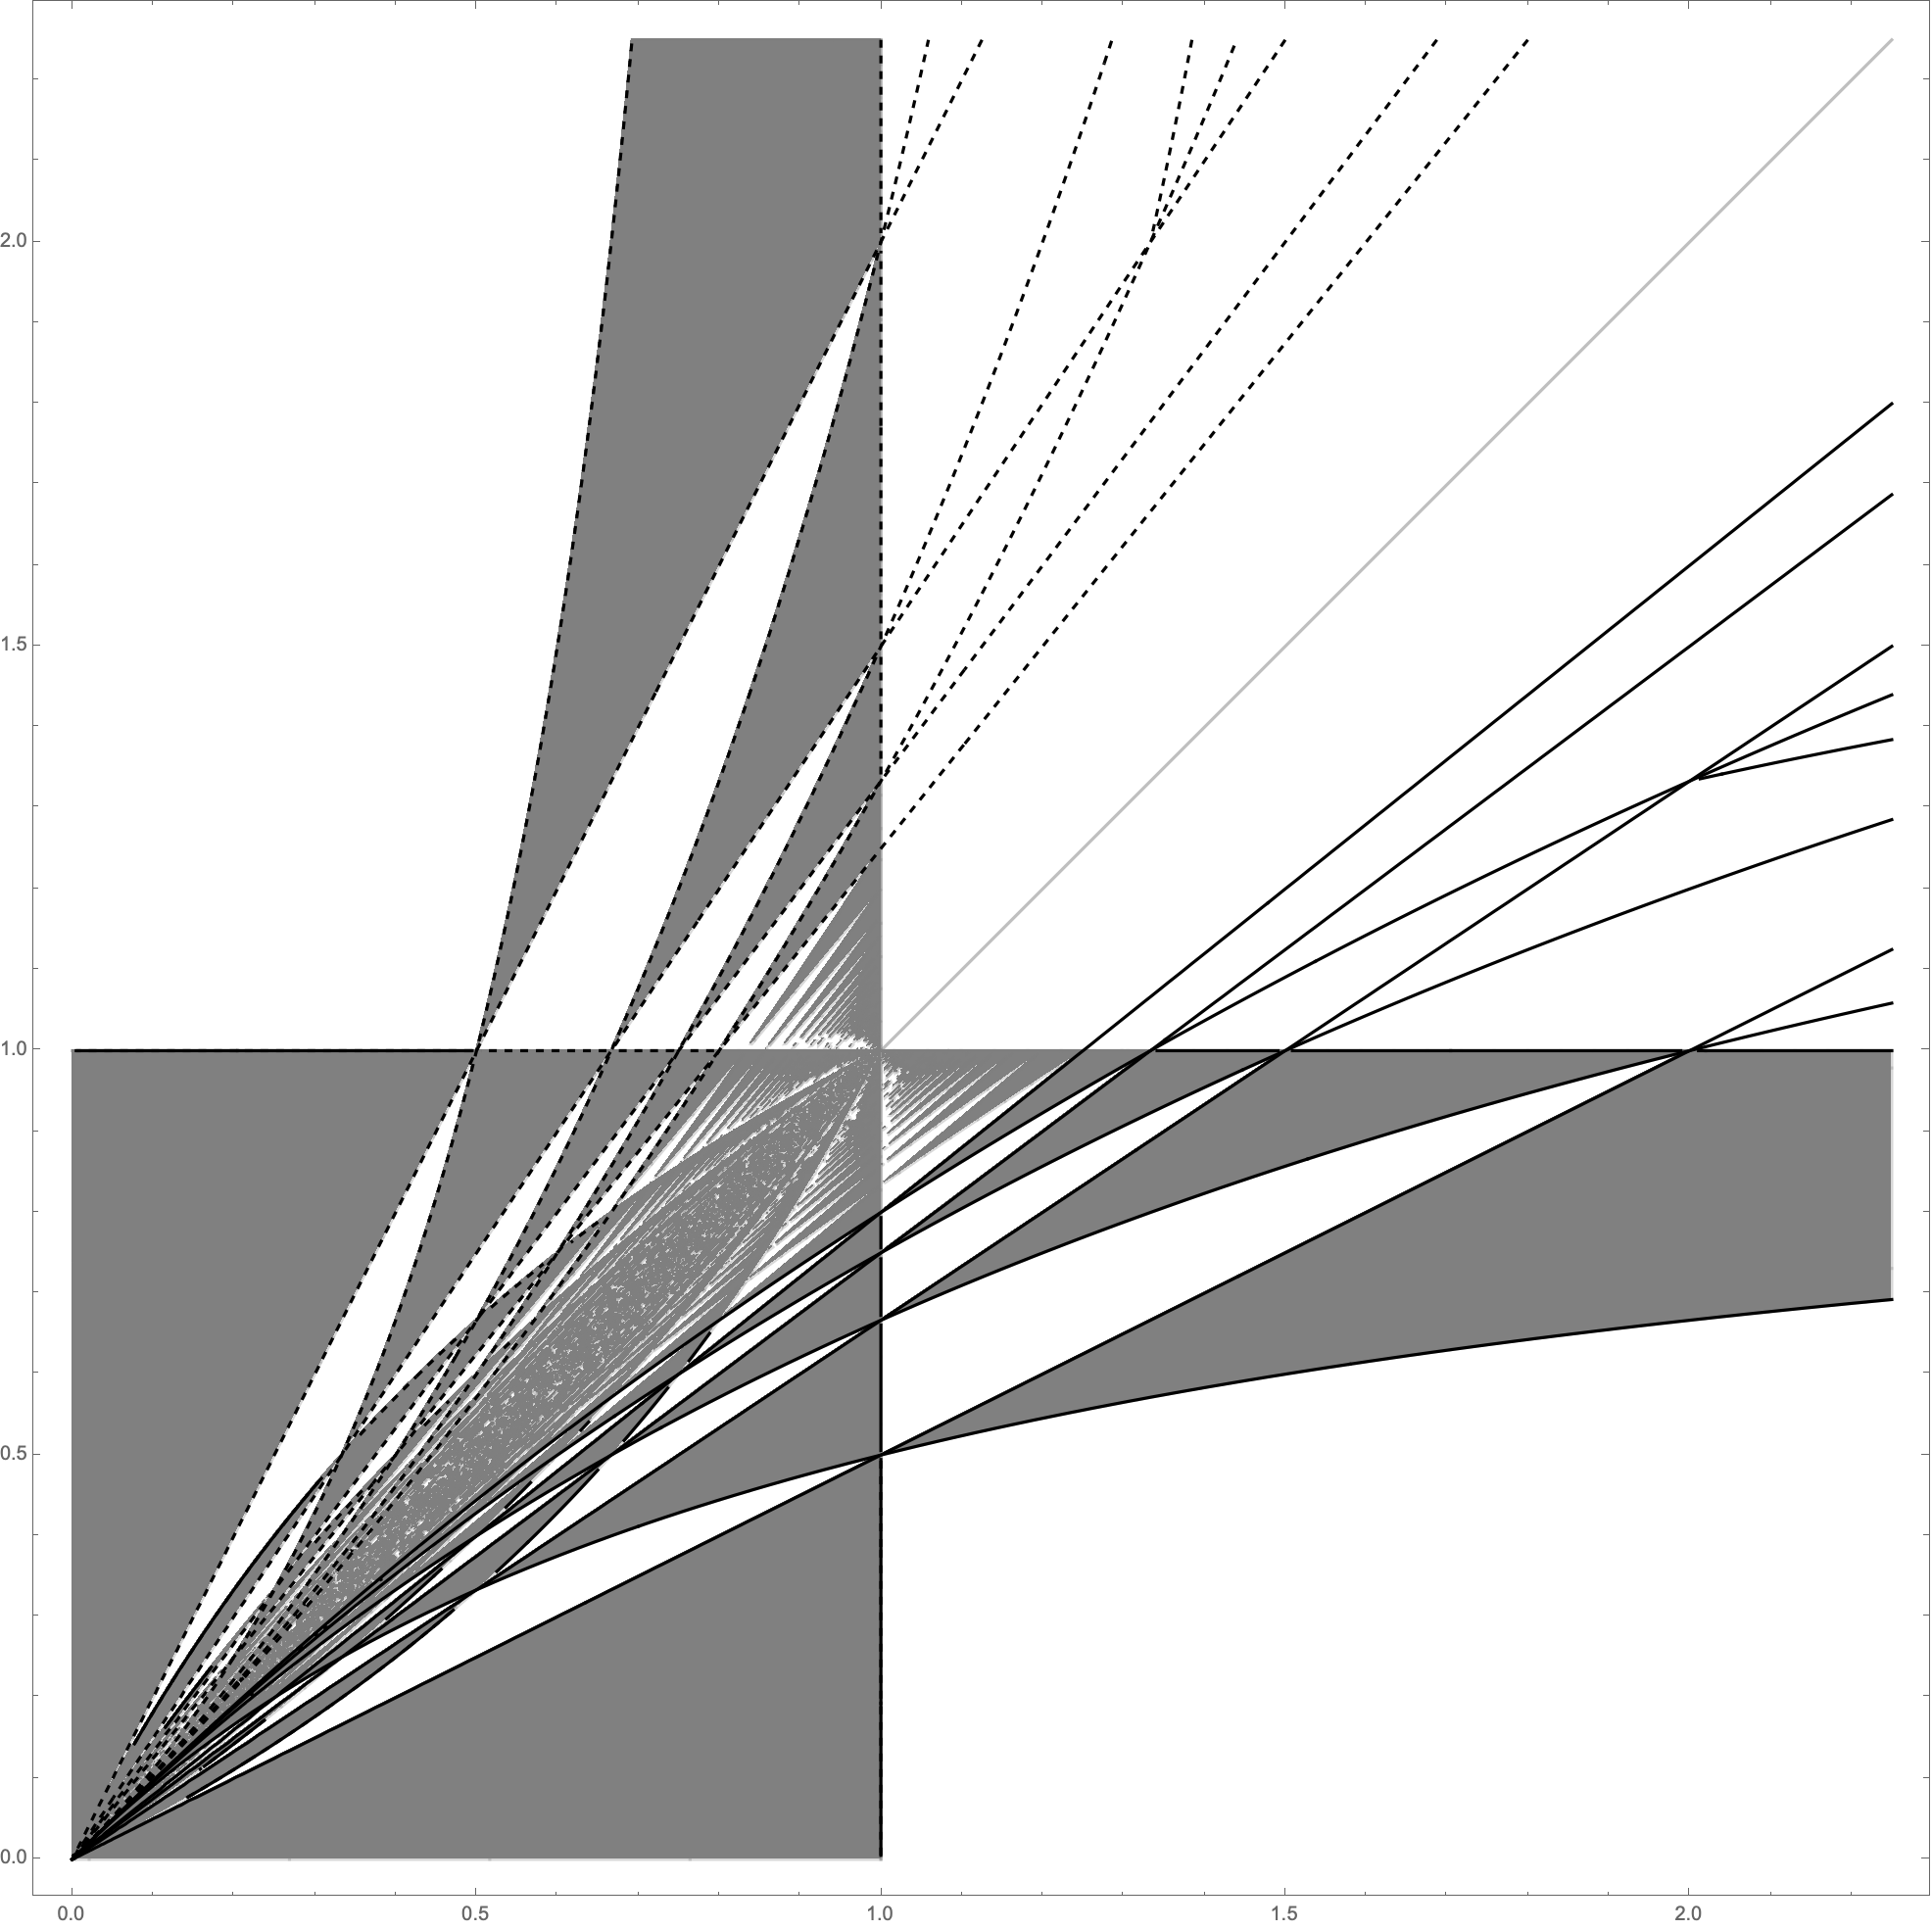
\includegraphics[width=6cm]{images/ch4/section3_circular/B1_lattice.png}
    \caption{Области $\left\{ \frac{\xi}{\gamma} \right\} < \frac{\varepsilon}{\gamma}$ (без штриховки) и  $\left\{ \frac{\xi}{\gamma} \right\} > \frac{\varepsilon}{\gamma}$ .}
    \label{fig:pt10:_B1_lattice}
\endminipage\hfill
\minipage{0.5\textwidth}
\centering
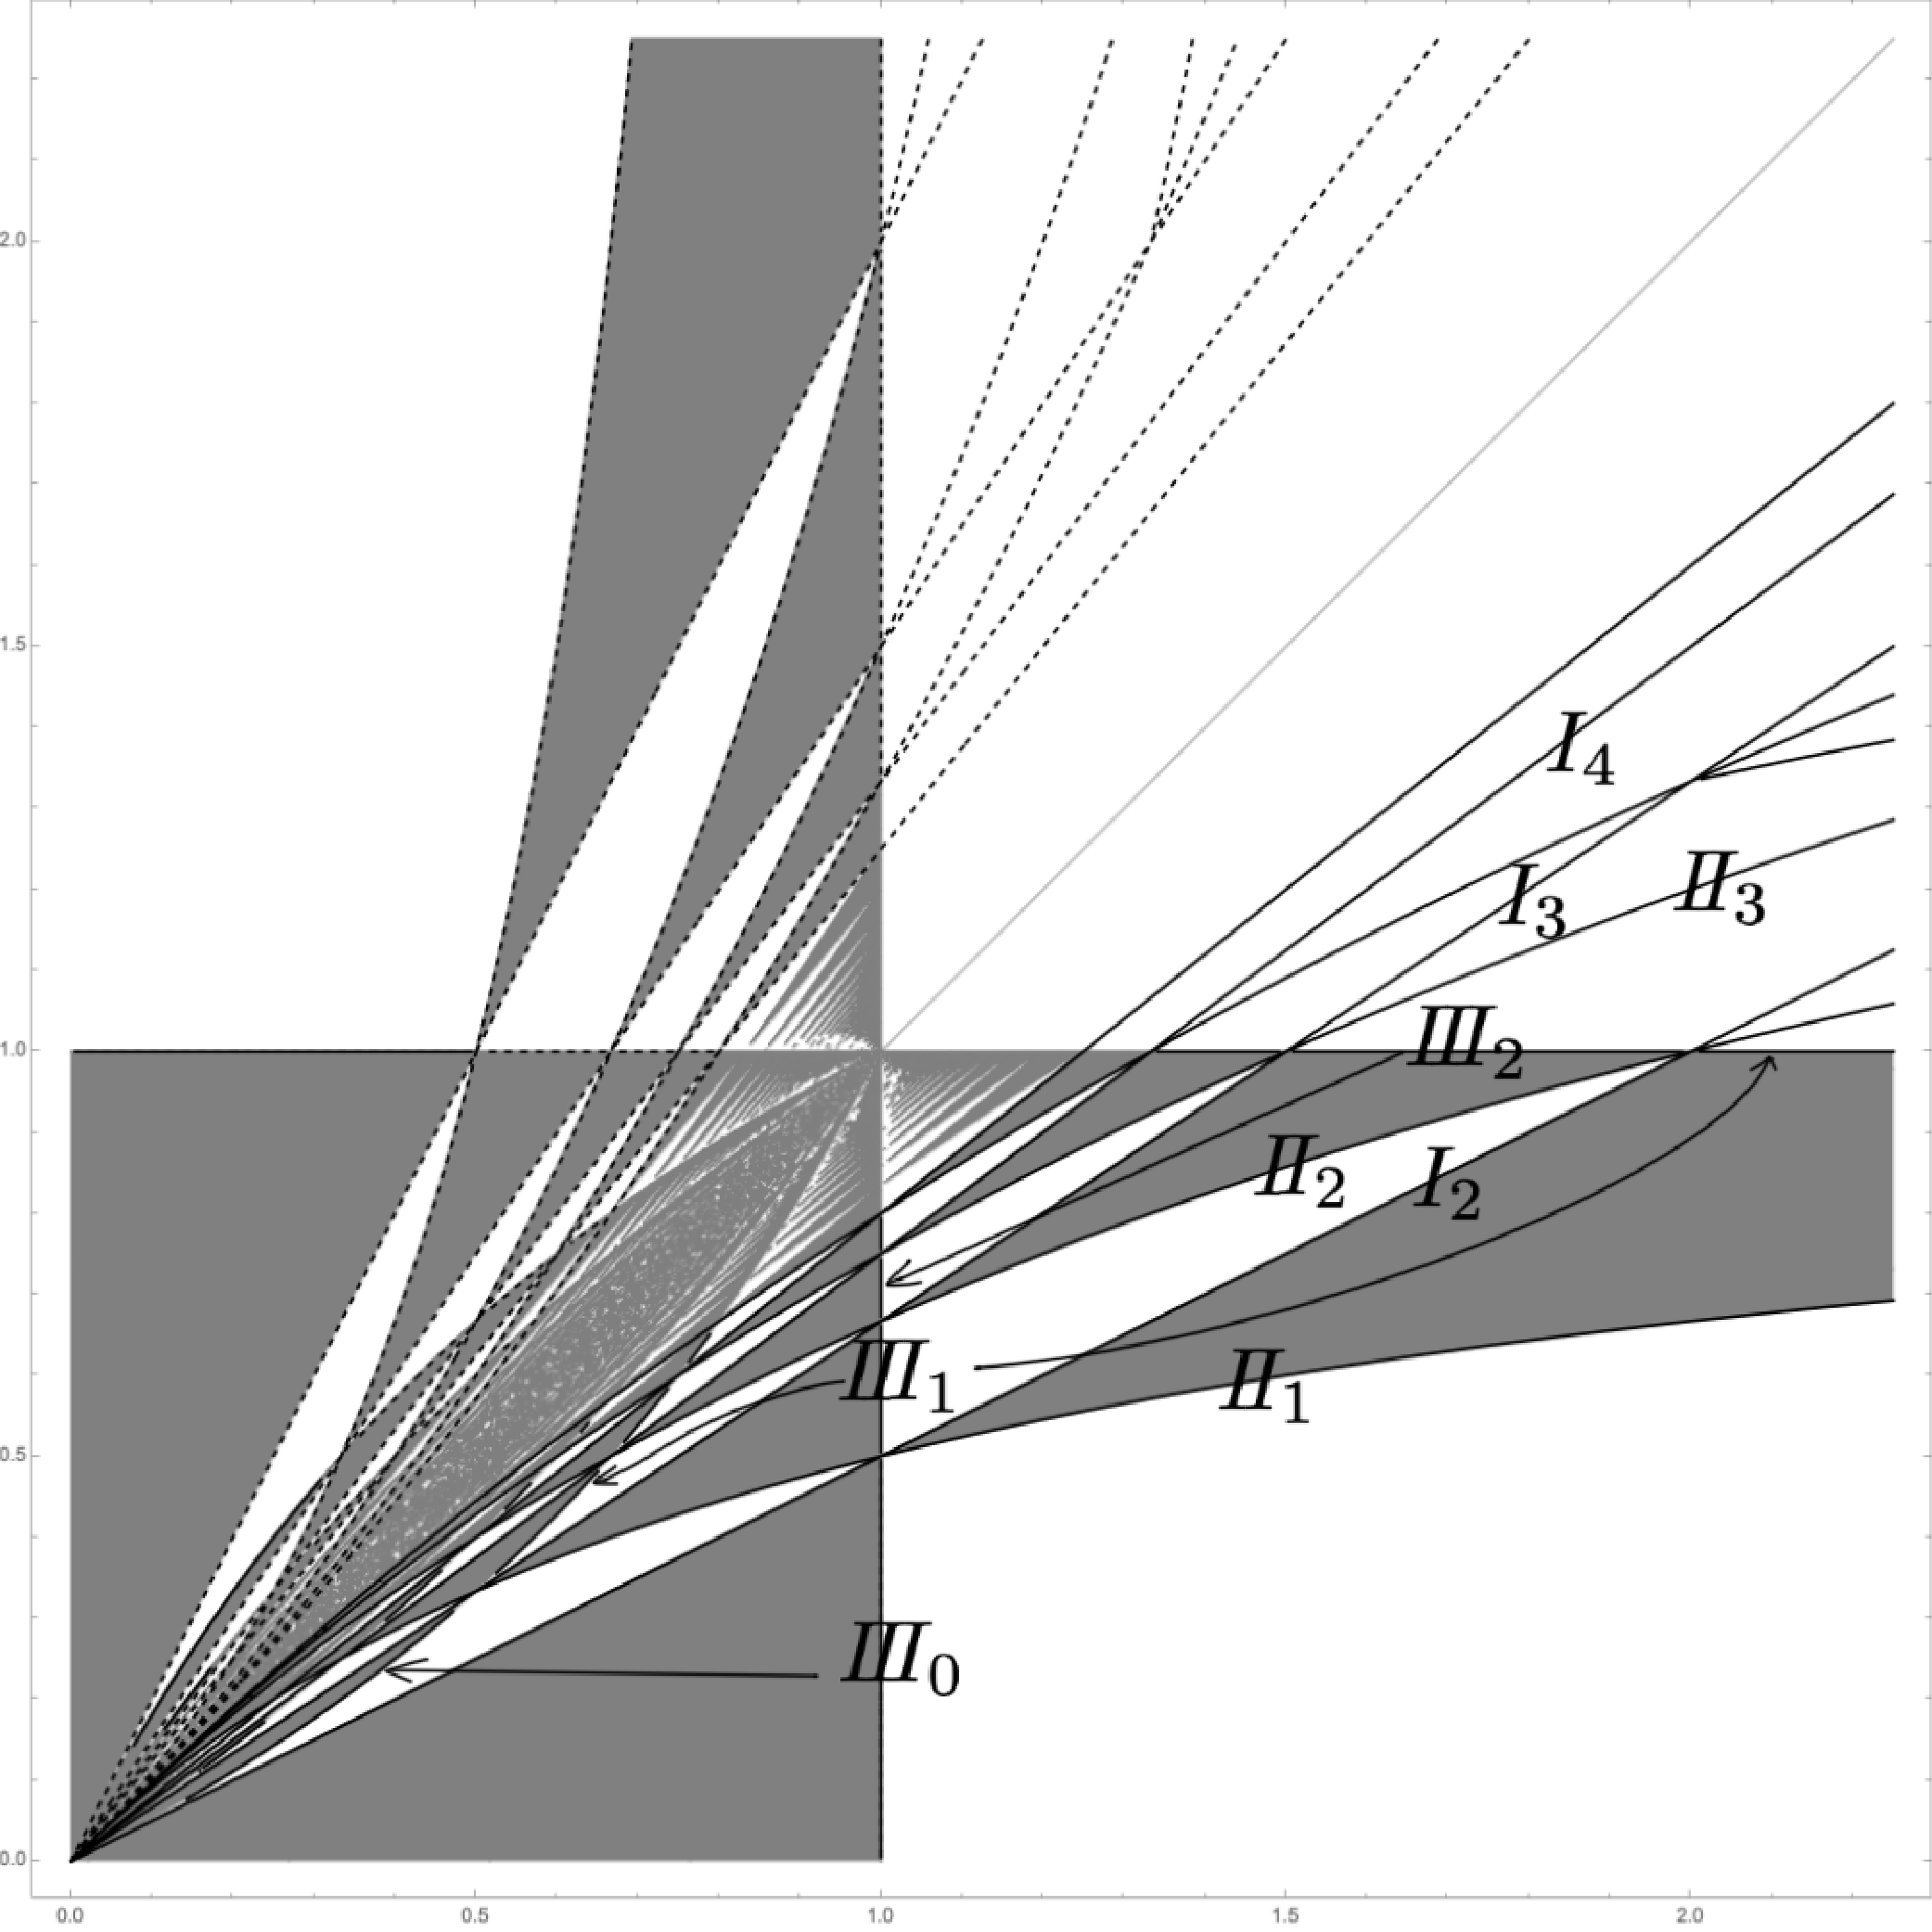
\includegraphics[width=6cm]{images/ch4/section3_circular/B1_lattice_labeled.pdf}
    \caption{Области с обозначениями некоторых граничных кривых.}
    \label{fig:pt10:_B1_lattice_labeled}
\endminipage\hfill
\end{figure}


Далее мы рассматриваем случай $n_1^2 < n_2^2$. Рассуждения для $n_1^2 > n_2^2$ аналогичны.

Введем обозначение $(x=\rho_1^2, y=\rho_2^2)$ в области $y < x, y < 1$ введем координаты $(\widetilde{x}, \widetilde{y})$ по формуле 
\begin{equation}
(\widetilde{x}, \widetilde{y}) = \left(\frac{x y }{(x-y) r_1^2}, \frac{x}{x-y}\right).
\label{eq:coord_change}
\end{equation}
Тогда приведенные в утверждении \ref{st:curves_formulas} уравнения можно переписать в следующем виде:

\begin{center}
\begin{tabular}{|c|c|c|c|}
\hline 
кривая & в координатах $(x,y)$  	& 	в координатах $(\widetilde{x},\widetilde{y})$				& 	параметр\\ \hline 
\hline 
$I_m$ 		& 	$y = \frac{m-1}{m} x$ 	& $\widetilde{y} = m$  		&	$m \geq 2$ \\ \hline 
$II_m$ 		&	$x y = m r_1^2 (x-y)$  	& $\widetilde{x}= m$ 		&	$m \geq 1$ \\ \hline 
$III_m$ 		&	$x y = r_1^2 (x-y) \left( m + \left\{\frac{x}{x-y}\right\}\right)$  & $\widetilde{x} = m + \left\{ \widetilde{y} \right\}$  	&	$m \geq 0$ \\ \hline 
\end{tabular}
\end{center}
Замена координат \eqref{eq:coord_change} обладает замечательным свойством: прямая $L$, которая задавалась уравнением \eqref{eq:lineL}: $y=\frac{n_1^2}{n_2^2} x$, переходит в прямую $\widetilde{L}: \left\{\widetilde{y} = \frac{n_2^2}{n_2^2-n_1^2} \right\}$.
Более того, несмотря на нелинейность замены координат \eqref{eq:coord_change}, сдвиг на вектор ${\gamma}_L$ вдоль прямой $L$ соответствует сдвигу на вектор $\widetilde{\gamma}_L = (1,0)$ вдоль прямой $\widetilde{L}$.
Чтобы не загромождать обозначения, далее вместо  $\widetilde{L}$ и $\widetilde{\gamma}_L$  будем  писать $L$ и $\gamma_L$; это не вызовет недоразумений.

Для фиксированных $n_1,n_2$ точка прямой $L$, соответствующая значениям интеграла $\Xi$, в старой системе координат пробегает отрезок от $(0, 0)$ до $P(\frac{r_1^2}{\sin \theta}) = \left(\frac{r_1^2}{\tg \theta}, r_1^2\right)$, а в новой системе координат --- от $\left(0,\frac{n_2^2}{n_2^2-n_1^2}\right)$ до $\left(\frac{n_2^2}{n_2^2-n_1^2}, \frac{n_2^2}{n_2^2-n_1^2}\right)$.
%В новой системе координат часть кривой $L \cap \left\{ \xi < L_1\right\}$ в соответствует координатной линии .
%Вектор $\gamma_L =  \overrightarrow{L_0 L_1}$ в новой системе координат соответствует вектору $\widetilde{\gamma}_L = (1,0)$.

Фрагмент диаграммы  \ref{fig:pt10:_B1_lattice} для $n_1 < n_2$ в новой системе координат изображен на рис. \ref{fig:pt10:_B1_lattice_straight}.
\begin{figure}[!htb]
\centering
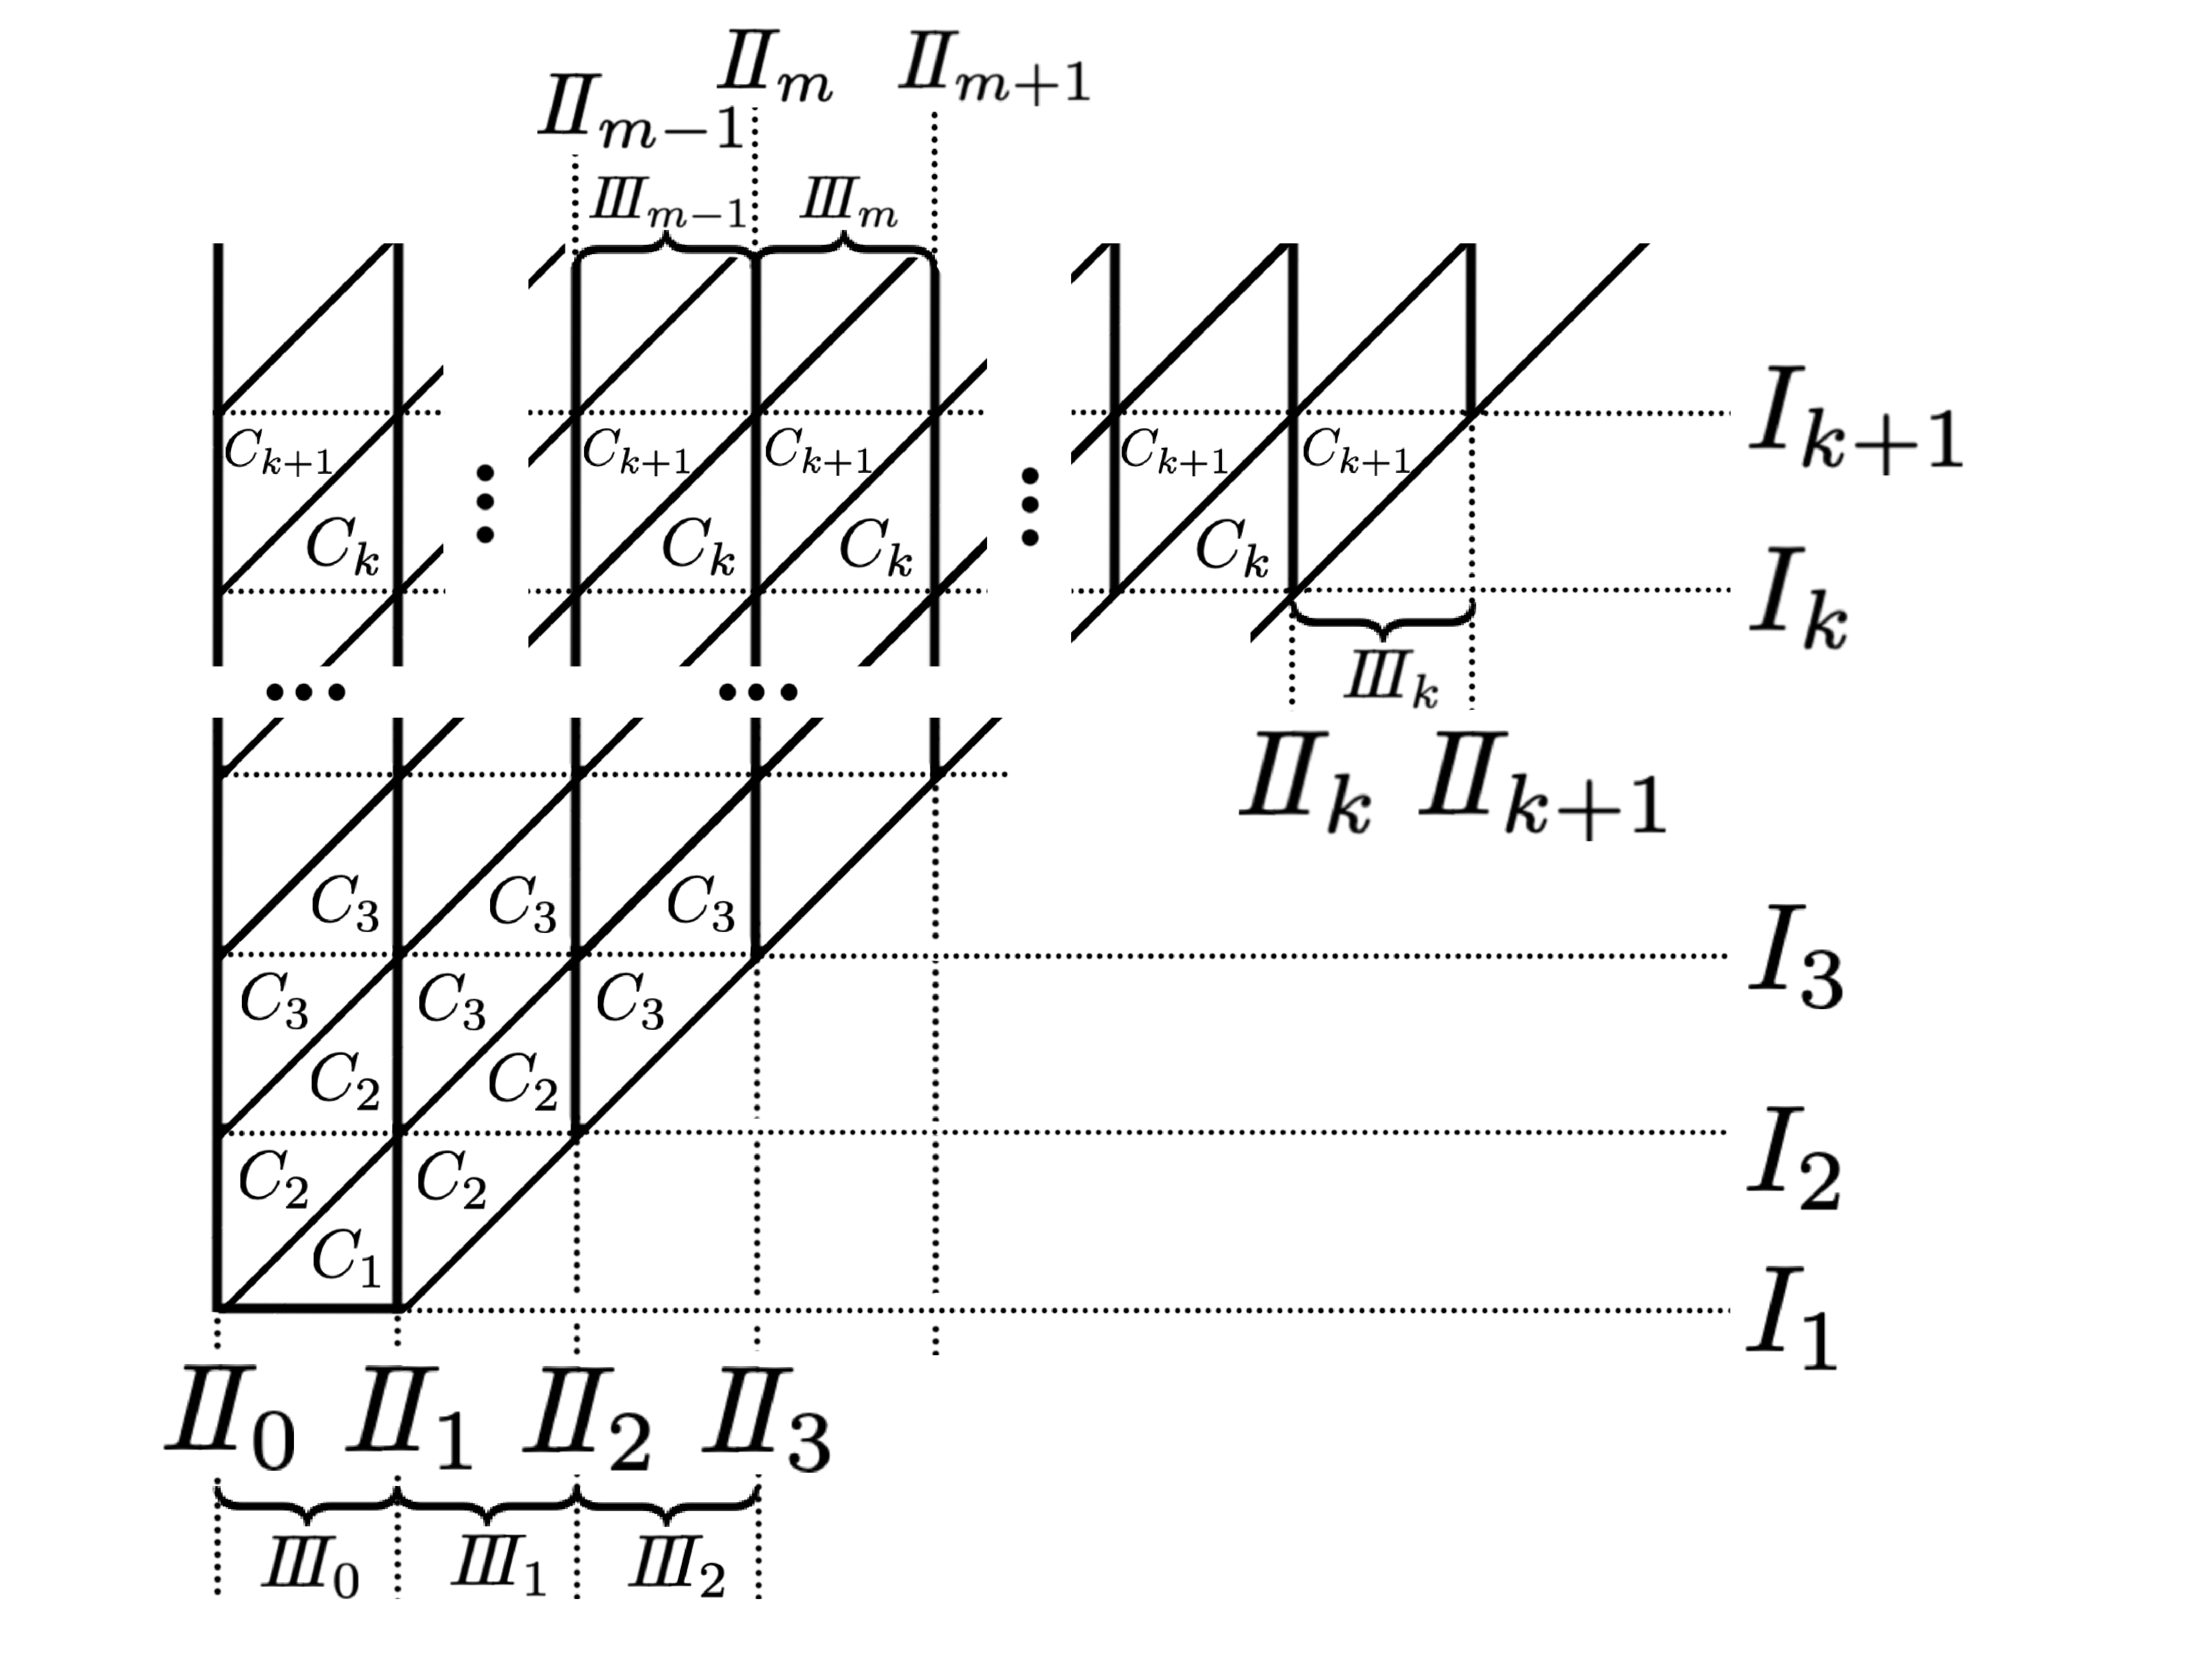
\includegraphics[width=10cm]{images/ch4/section3_circular/B1_lattice_straight.pdf}
    \caption{}
    \label{fig:pt10:_B1_lattice_straight}
\end{figure}

%На приведенной диаграмме кривые семейства $I$ являются горизонтальными прямыми, кривые семейства $II$ представляют собой вертикальные прямые, а каждая кривая семейства $III$ выглядит как кусочно линейная кривая, ограниченная между двумя кривыми $II_m, II_{m+1}$ семейства $II$. 
%Прямая $L$ в изображенной на рис. \ref{fig:pt10:_B1_lattice_straight} диаграмме проходит горизонтально и заключена между прямыми $I_k$ и $I_{k+1}$. 
%Коэффициент $\gamma$ на этой диаграмме имеет постоянную величину для всех $n_1^2, n_2^2$. 
%Точка на $L$, соответствующая паре $(\rho_1^2, \rho_2^2)$, при переходе траектории через дугу $EF$ из области $\Omega_2$ в $\Omega_1$ соответствует сдвигу вдоль прямой $L$ на вектор $\gamma_L = \left(1,0\right)$. Тогда видно, что если точка принадлежала множеству класса $C_m$, то после сдвига она попадает в другое множество того же класса $C_m$.
%При этом возможно только конечное количество сдвигов на вектор $\gamma_L$ вдоль кривой $L$. 

\begin{remark}
Заметим, что на рис. \ref{fig:pt10:_B1_lattice_straight} появляются новые прямые $II_0$ и $I_1$, которые отсутствовали на рис. \ref{fig:pt10:_B1_lattice}. Они введены для удобства и продолжают определения из уравнения \eqref{eq:families_def}. Кривая $II_0$ соответствует (см. утверждение \ref{st:curves_formulas} и определение координат $\widetilde{x}, \widetilde{y}$) случаю, когда $\rho_1^2 = 0$ или $\rho_2^2 = 0$. Кривая $I_1$ соответствует предельному случаю при $n_1 \to 0$, который не соответствует бильярду с законом преломления $(\ast)$.
\end{remark}

\section{Классификация фрагментов  $T_m$ бильярдной траектории}
Фрагменты  $T_m$ произвольной траектории можно разделить на те, которые допускают преломление через дугу $EF$ в обоих направлениях (1) и на те, которые допускают переход через $EF$ только в одном направлении  (2). Последние, в свою очередь, могут допускать переход либо только в сторону увеличения интеграла $\Xi$ (2a), либо только в сторону его уменьшения (2b).

Эти три случая описываются следующим образом в терминах значения интеграла $\Xi$:
%А именно, для $\Xi$ как параметра на произвольной $L$:

(1) При $\Xi \in (\gamma, ||L_1|| - \gamma)$ величина $\Xi \pm \gamma$ остается в пределах $(0, ||L_1||)$, где определены обе каустики;

(2) В противном случае угол $\theta$ для преломленного луча не определен:

$\quad $(2a) При пересечении $EF$ в сторону уменьшения $\Xi$ при $\Xi < \gamma$, поскольку должно выполняться неравенство $\cos^2 \theta > 1$;

$\quad $(2b) При пересечении $EF$ в сторону увеличения $\Xi$ при $\Xi > ||L_1|| - \gamma$, поскольку должно выполняться неравенство $\cos^2 \theta < 0$. В частности, этому случаю соответствует $\rho_1 > r_1$.

Равенство $\Xi = \gamma$ для произвольной прямой $L$ эквивалентно ее пересечению с кривой $II_1$ (см. \ref{eq:families_def}). Аналогично равенство $\Xi = ||L_1||-\gamma$ эквивалентно пересечению $L$ с кривой $\widehat{III}$, составленной из сегментов кривых $III_{k-1}$. 
%\textcolor{red}{===ниже утверждение в виде, который мне не нравится===}
%
%Будет полезно следующее утверждение:
%\begin{statement}
%Пусть $L$ расположена между $I_k$ и $I_{k+1}$ и $\xi \in L$ --- точка на этой прямой, соответствующая радиусам каустик $(\rho_1^2, \rho_2^2) = P(\xi)$. 
%
%Тогда если $\xi < \widetilde{\xi}_{II_1} = L \cap II_1$ или $\xi > \widetilde{\xi}_{III_{k-1}} = L \cap III_{k-1}$, то траектории могут перейти через ребро $EF$ только в одном направлении. В противном случае траектории могут преломиться проходить через ребро $EF$ в обоих направлениях.
%\end{statement}
%\textcolor{red}{===ниже утверждение в виде, который мне не нравится===}
Для наглядности кривые показанына рис. \ref{fig:pt10:_B1_lattice_straight_with_line}.
\begin{figure}[!htb]
\centering
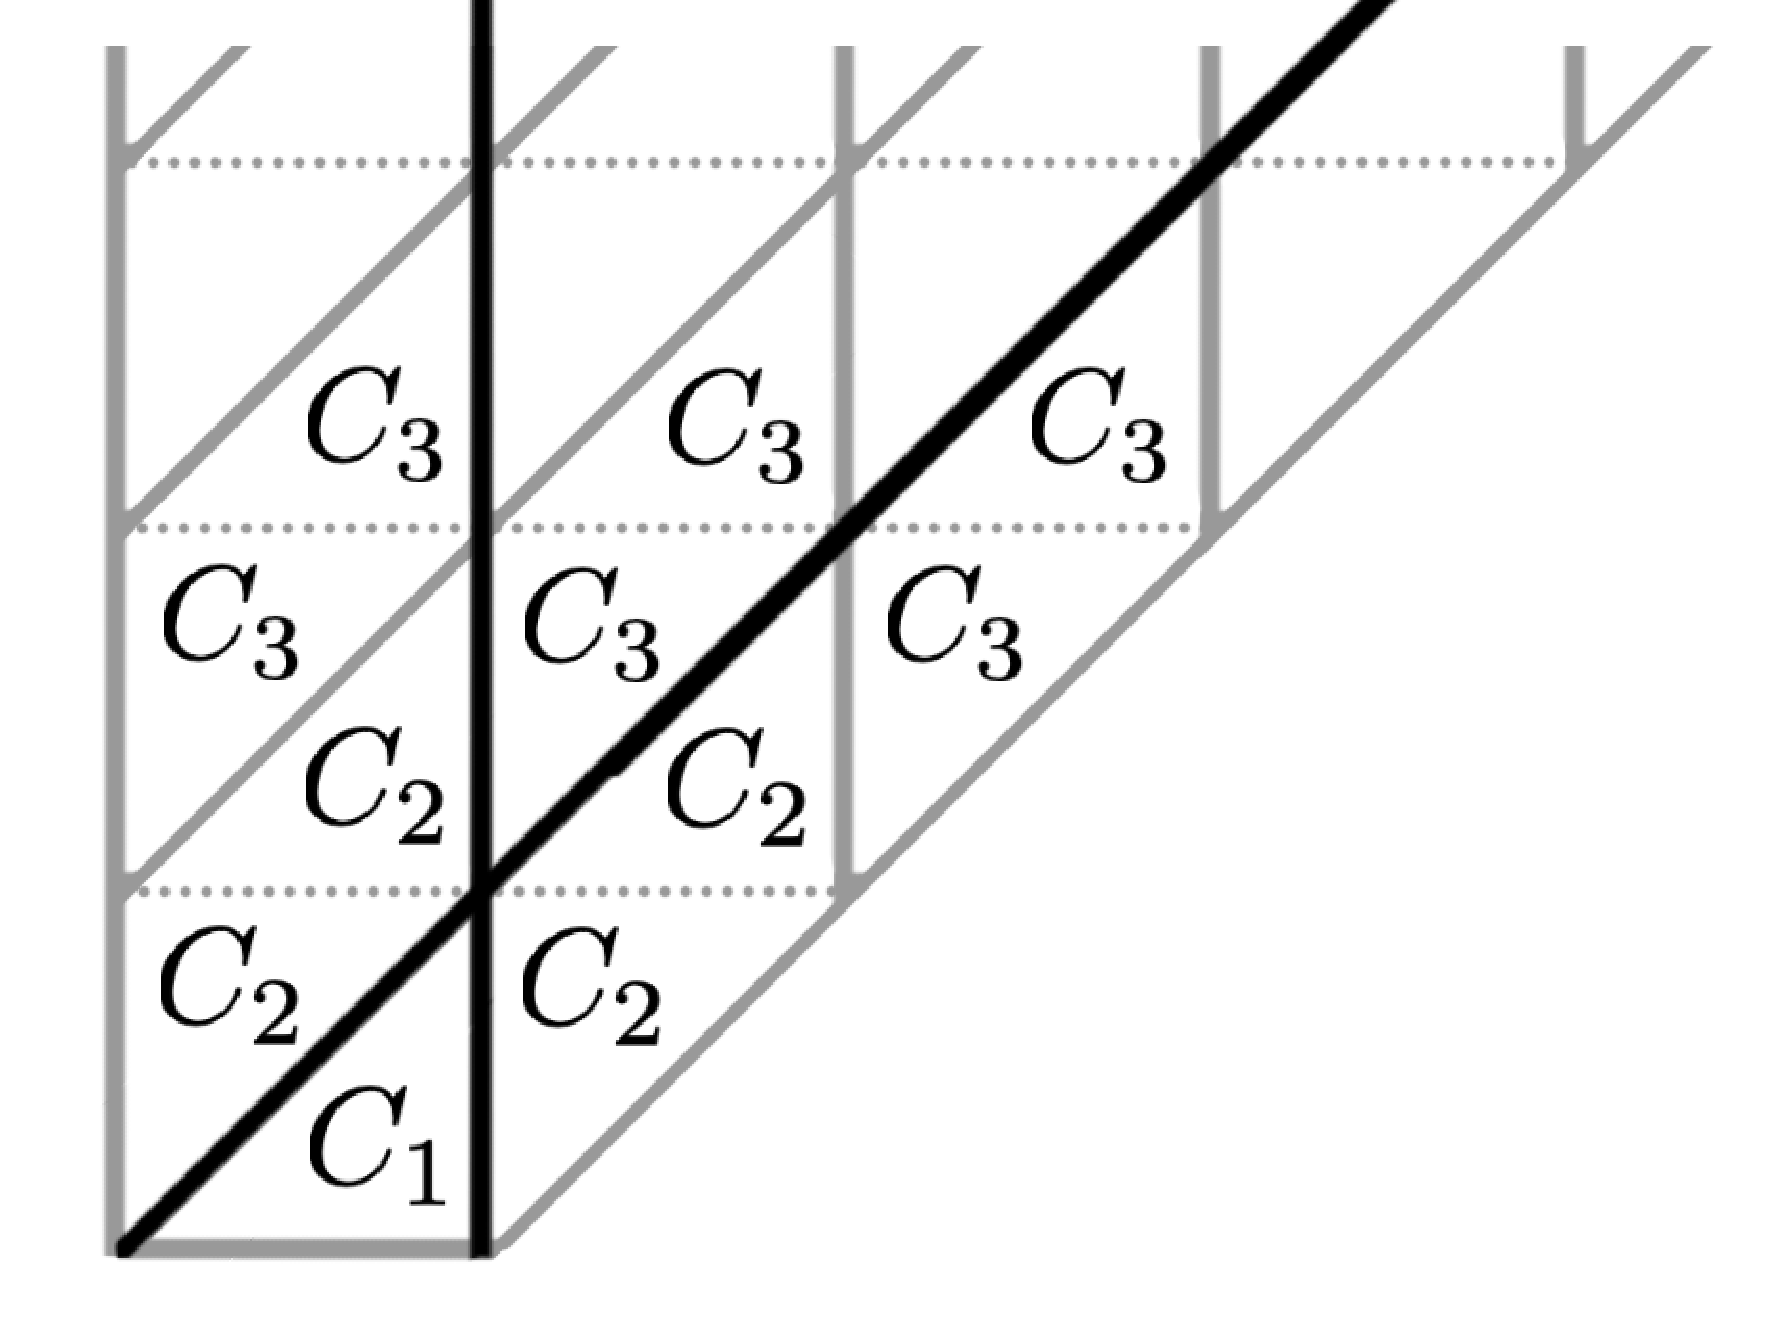
\includegraphics[width=4cm]{images/ch4/section3_circular/B1_lattice_straight_with_line.pdf}
    \caption{Кривые $II_1$ и $\widehat{III}$.}
    \label{fig:pt10:_B1_lattice_straight_with_line}
\end{figure}
%\begin{proof}
%Пусть $\xi < \widetilde{\xi}_{II_1} = L \cap II_1$, то есть $\xi < \gamma$. 
%Подставим в последнее неравенство выражения для $\xi$ и $\gamma$ через квадраты радиусов каустик $\rho_1^2, \rho_2^2$ и $\theta$, что позволит записать его в виде
%$ \frac{\rho_2^2}{\sin \theta} < r_1^2 \left( \frac{1}{\sin \theta} - \frac{1}{\cos \theta} \right)$.
%Неравенство можно привести к виду 
%$$(\rho_2^2 - r_1^2) \frac{\cos \theta}{\sin \theta} + r_1^2 = 
%(\rho_2^2 - r_1^2) \frac{n_2^2}{n_1^2} + r_1^2 < 0.$$
%Согласно формуле из утверждения \ref{st:across_EF}, эта величина является квадратом радиуса каустики $\widetilde{\rho}_1^2$ в области $\Omega_1$ при переходе из области $\Omega_2$ через дугу $EF$. 
%Квадрат радиуса не может являться строго отрицательной величиной, следовательно каустика не будет определена. В частности, для траектории это значит, что она должна будет отразиться от дуги $EF$ обратно в область $\Omega_2$. 

%Пример траектории изображен на рис. \ref{fig:pt10:_terminal_min_domain}.

%Пусть $\xi > \widetilde{\xi}_{III_{k-1}} = L \cap III_{k-1}$, то есть $\xi > (k-1) \gamma + \varepsilon$. 
%Последнее неравенство с подстановкой $\varepsilon$ упрощается до вида  
%$\xi >  ||L_1|| - \gamma$. Перепишем его через $\rho_1^2$ и $\theta$, получим 
%$$\frac{\rho_1^2}{\cos \theta} > \frac{r_1^2}{\sin \theta} - \left( \frac{r_1^2}{\sin \theta} - \frac{r_1^2}{\cos \theta} \right) =  \frac{r_1^2}{\cos \theta},$$
%следовательно $\rho_1^2 > r_1^2$, поскольку $\cos \theta > 0$. Для траектории это означает, что траектория в области $\Omega_1$ лежит снаружи окружности, содержащей ребро $EF$ и не сможет его пересечь. 
%Пример траектории при $\rho_1 < r_2$ изображен на рис. \ref{fig:pt10:_terminal_max_domain}.
%\end{proof}

Кривые $II_1$ и $\widehat{III}$ разбивают диаграмму, изображенную на рис. \ref{fig:pt10:_B1_lattice_straight_with_line} на четыре части.
Поведение фрагмента бильярдной траектории на дуге $EF$ можно описать, зная какой из четырех частей принадлежит значение интеграла $\Xi$, соответствующее этому фрагменту.

$\bullet$ Для точек левее $II_1$ невозможно преломление с уменьшением $\Xi$, поэтому (см. рис.     \ref{fig:n1ltn2_Xi_growth}) траектория в области $\Omega_2$ отражается от $EF$.

$\bullet$ Для точек правее $\widehat{III}$ радиус каустики $\rho_1$ превосходит радиус $r_1$ окружности, содержащей дугу $EF$, потому траектория не может пересечь эту дугу в области $\Omega_1$.

Для траекторий, соответствующих точкам правее $\widehat{III}$, поведение фрагмента траектории можно уточнить:
а именно, рассмотрим  $IV_0$ как фрагмент прямой $\widetilde{y} = \widetilde{x}\dfrac{r_1^2}{r_2^2} + 1$ в области $\{ \widetilde{x}> 0\} \cap \{\widetilde{y}< \frac{r_2^2}{r_2^2-r_1^2} \}$.

$\bullet$ Тогда для точек правее $IV_0$ соответствующий фрагмент траектории в области $\Omega_2$ отражается от ребра $FG$.

%При этом из последнего случая можно выделить особенность, когда прямая $L$ пересекает   координатную линию $x =r_2^2$ в области $\{\xi < L_1\}$. Эта координатная линия в координатах $(\widetilde{x}, \widetilde{y})$ задается равенством $\widetilde{y} = \widetilde{x}\frac{r_1^2}{r_2^2} + 1$.
%Неравенство $y < r_1^2$, соответствующее условию $\xi < L_1$, запишем в новых координатах в виде $\dfrac{\widetilde{x}}{\widetilde{y}} \in (0, 1)$.
%Тогда можно определить прямую 
% Можно определить $IV$ семейство кривых, соответствующих уравнениям $IV_m = \left\{ \widetilde{y} = (\widetilde{x} + m) \frac{r_1^2}{r_2^2} + 1 \right\}$.  
На рис. \ref{fig:pt10:_B1Prime_lattice} изобразим диаграмму \ref{fig:pt10:_B1_lattice_straight_with_line}, дополненную отрезком $IV_0$.


\begin{figure}[!htb]
\centering
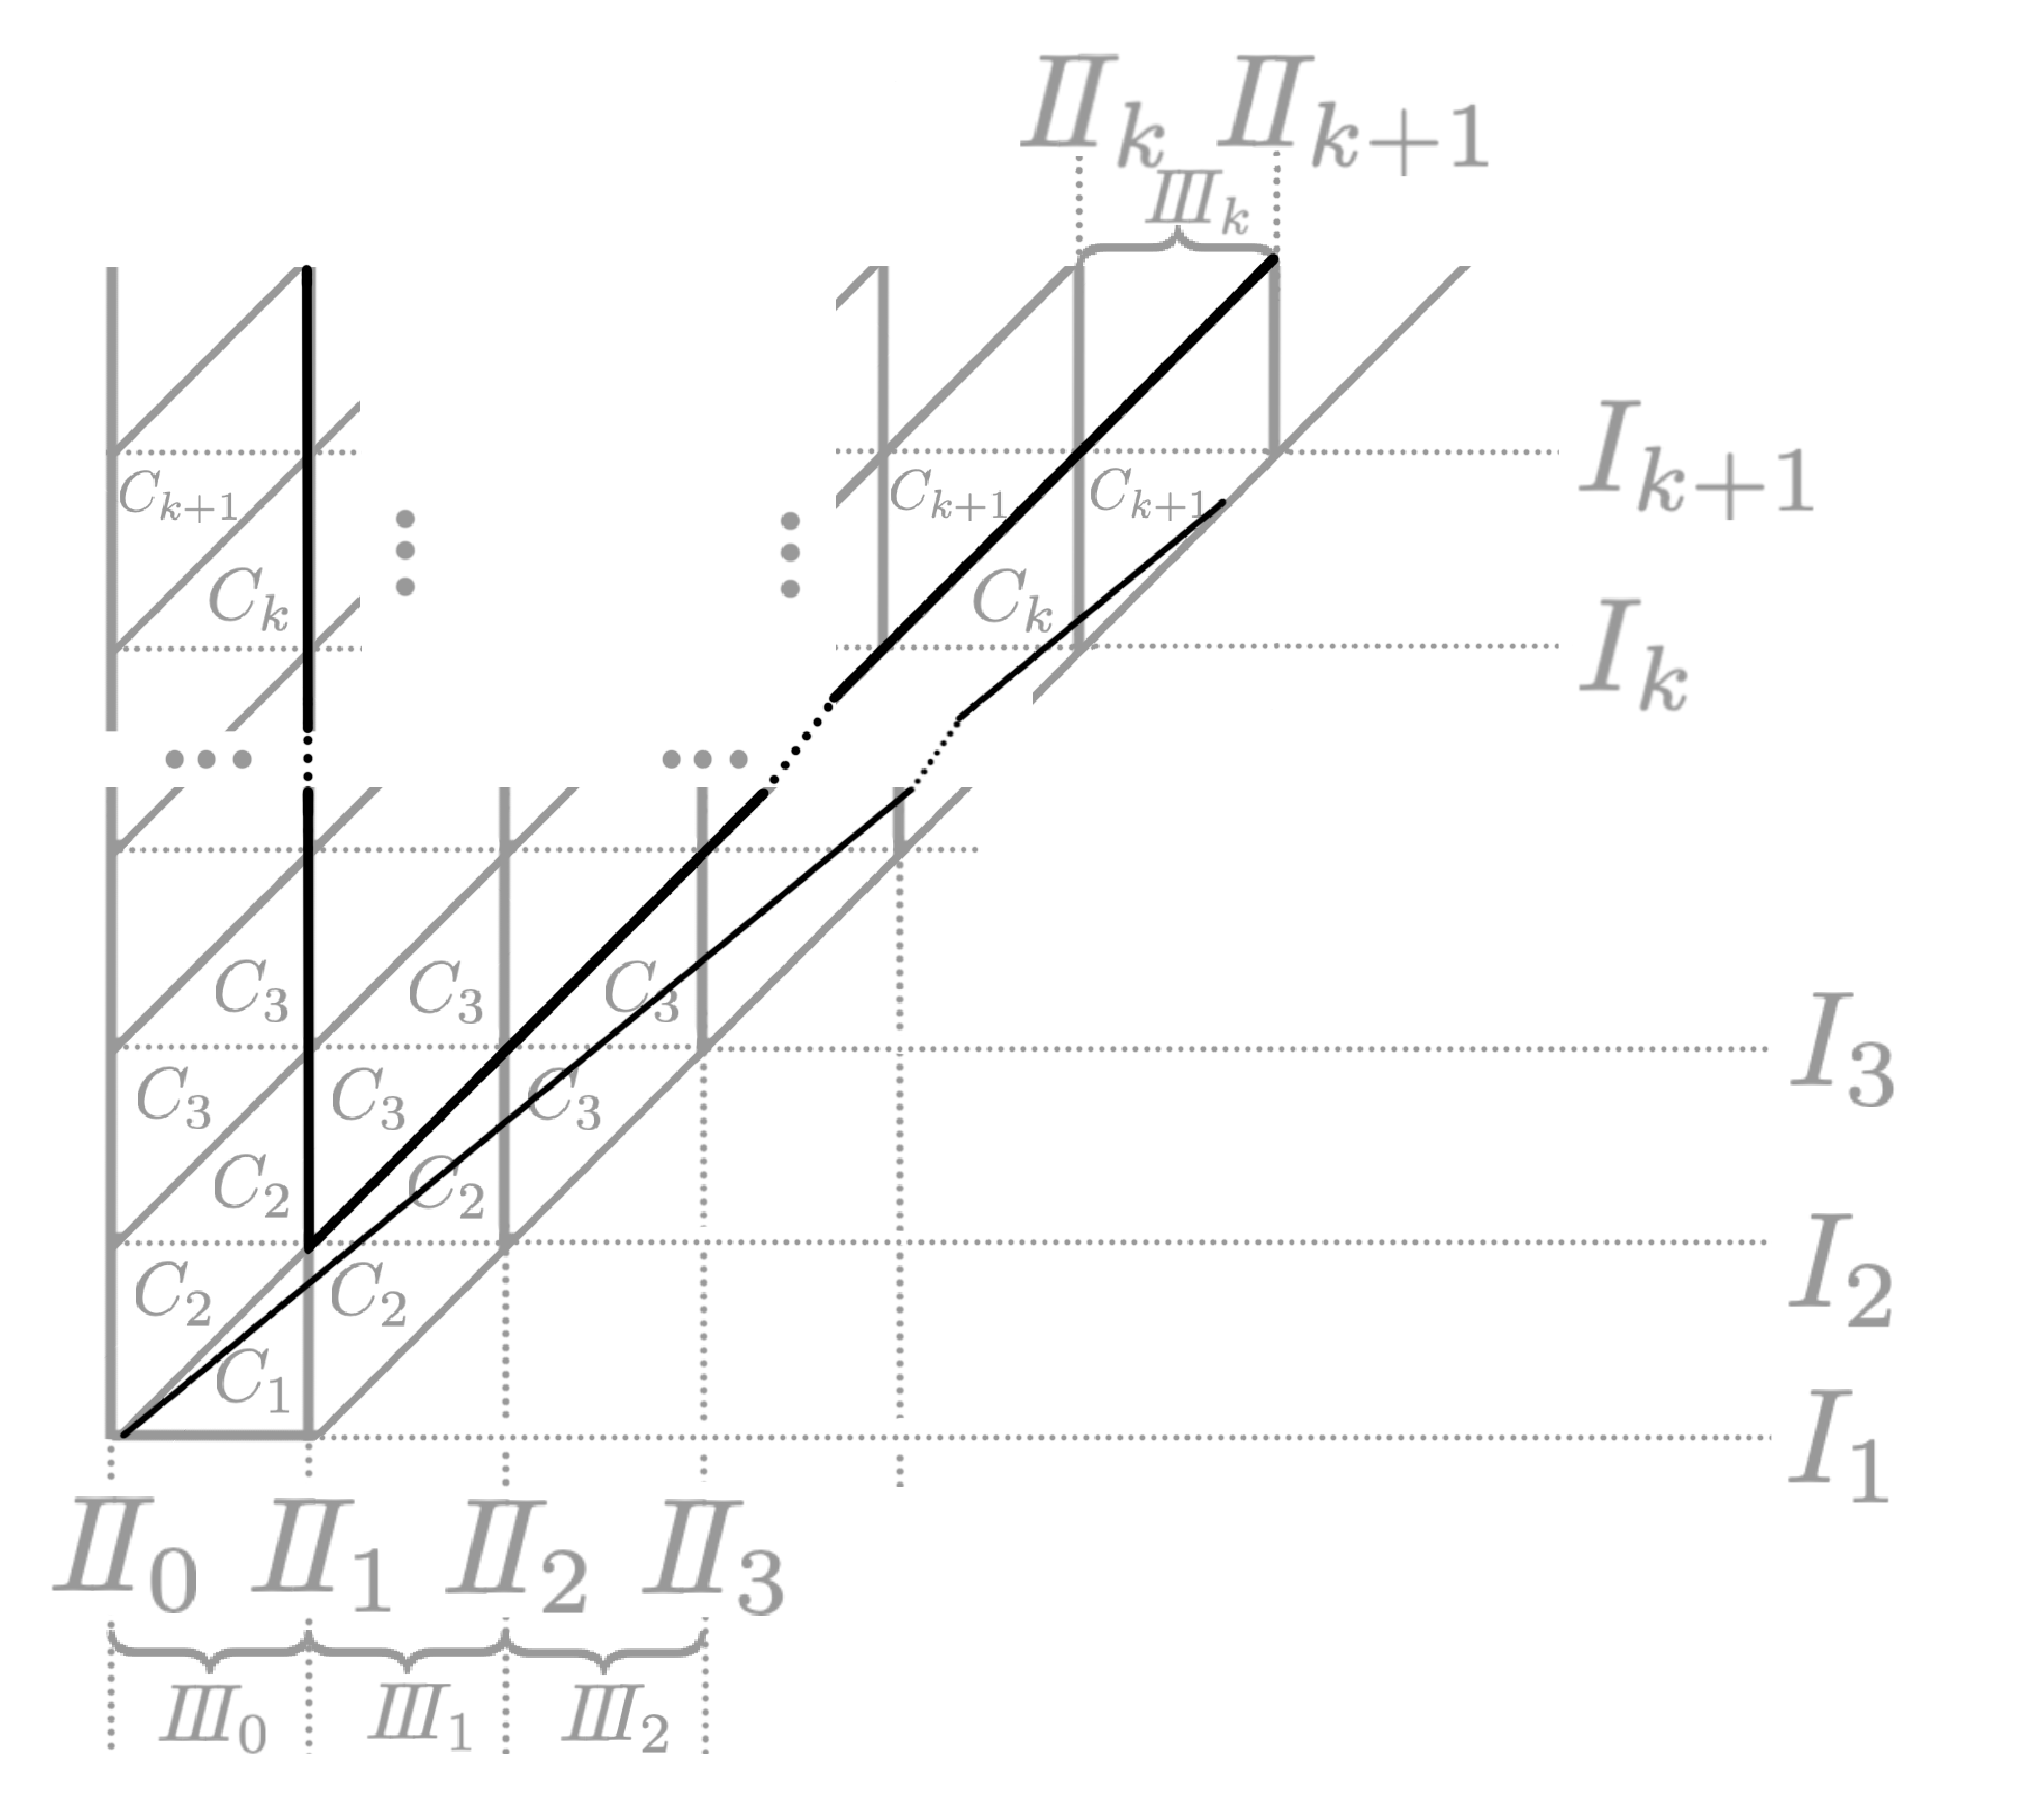
\includegraphics[width=7cm]{images/ch4/section3_circular/B1Prime_lattice.pdf}
    \caption{Прямая, соответствующая прямой $\rho_1^2 = r_2^2$.}
    \label{fig:pt10:_B1Prime_lattice}
\end{figure}
%Таким образом, предыдущие два пункта для $II_1$ и $\widehat{III}$ можно дополнить еще одним случаем:


Из вышесказанного справедливо следующее:
\begin{statement}
Пусть $n_1 < n_2$. Рассмотрим произвольную точку $Q$ в области $\{ \xi < L_1 \}$.
Тогда, в зависимости от расположения точки $Q$ относительно кривых $II_1$, $\widehat{III}$ и $IV_0$, всевозможные фрагменты $T_m$ бильярдных траекторий, соответствующие точке $Q$, заметают следующие области:

$\bullet$ изображенную на рис. \ref{fig:pt10:_terminal_min_domain}, если точка $Q$  \textbf{левее} $II_1$ и \textbf{левее} $\widehat{III}$.

$\bullet$ изображенную на рис. \ref{fig:pt10:_branching_domain}, если точка  $Q$  \textbf{правее} $II_1$ и \textbf{левее} $\widehat{III}$.

$\bullet$ изображенную на рис. \ref{fig:pt10:_terminal_max_domain}, если точка   $Q$ \textbf{правее} $II_1, \widehat{III}$ и \textbf{левее} $IV_0$.

$\bullet$ изображенную на рис.  \ref{fig:pt10:_C1_domain}, если точка  $Q$  \textbf{левее} $II_1$, $IV_0$ и \textbf{правее} $\widehat{III}$.

$\bullet$ изображенную на рис. \ref{fig:pt10:_terminal_max_domain_B1Prime}, если точка   $Q$ \textbf{правее} $II_1$ и $IV_0$.

$\bullet$ изображенную на рис.  \ref{fig:pt10:_C1_domainPrime}, если точка  $Q$ \textbf{левее} $II_1$ и  \textbf{правее} $IV_0$.

При этом случаям, показанным на рис. \ref{fig:pt10:_C1_domain}, \ref{fig:pt10:_C1_domainPrime}, соответствует только множество $C_1$, остальным соответствуют множества $C_k, k\geq 2$.
\label{stat:domain_shapes}
\begin{figure}[!htb]
\minipage{0.25\textwidth}
\centering
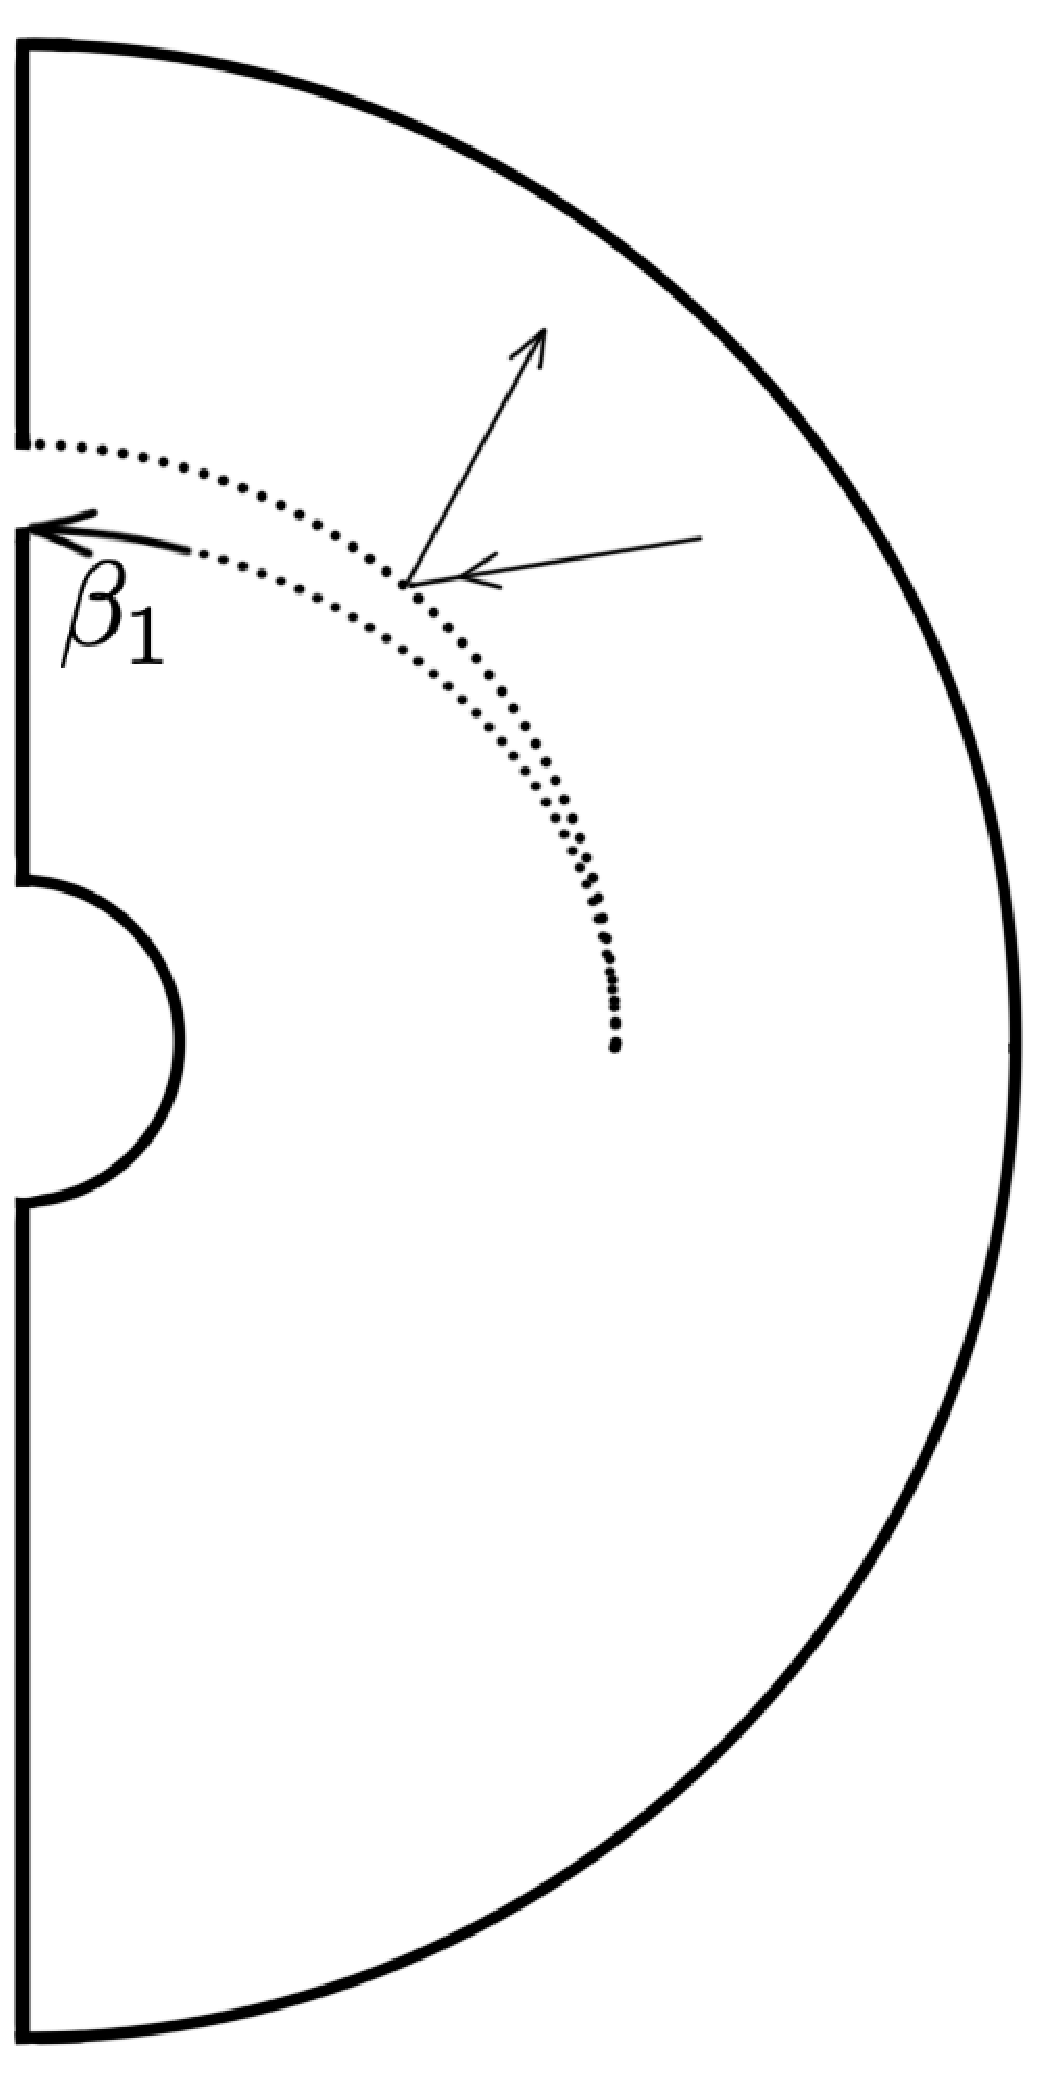
\includegraphics[width=2cm]{images/ch4/section3_circular/atoms/branching/terminal_min.pdf}
    \caption{\textbf{левее} $II_1$ и \textbf{левее} $\widehat{III}$.}
    \label{fig:pt10:_terminal_min_domain}
\endminipage\hfill
\minipage{0.25\textwidth}
\centering
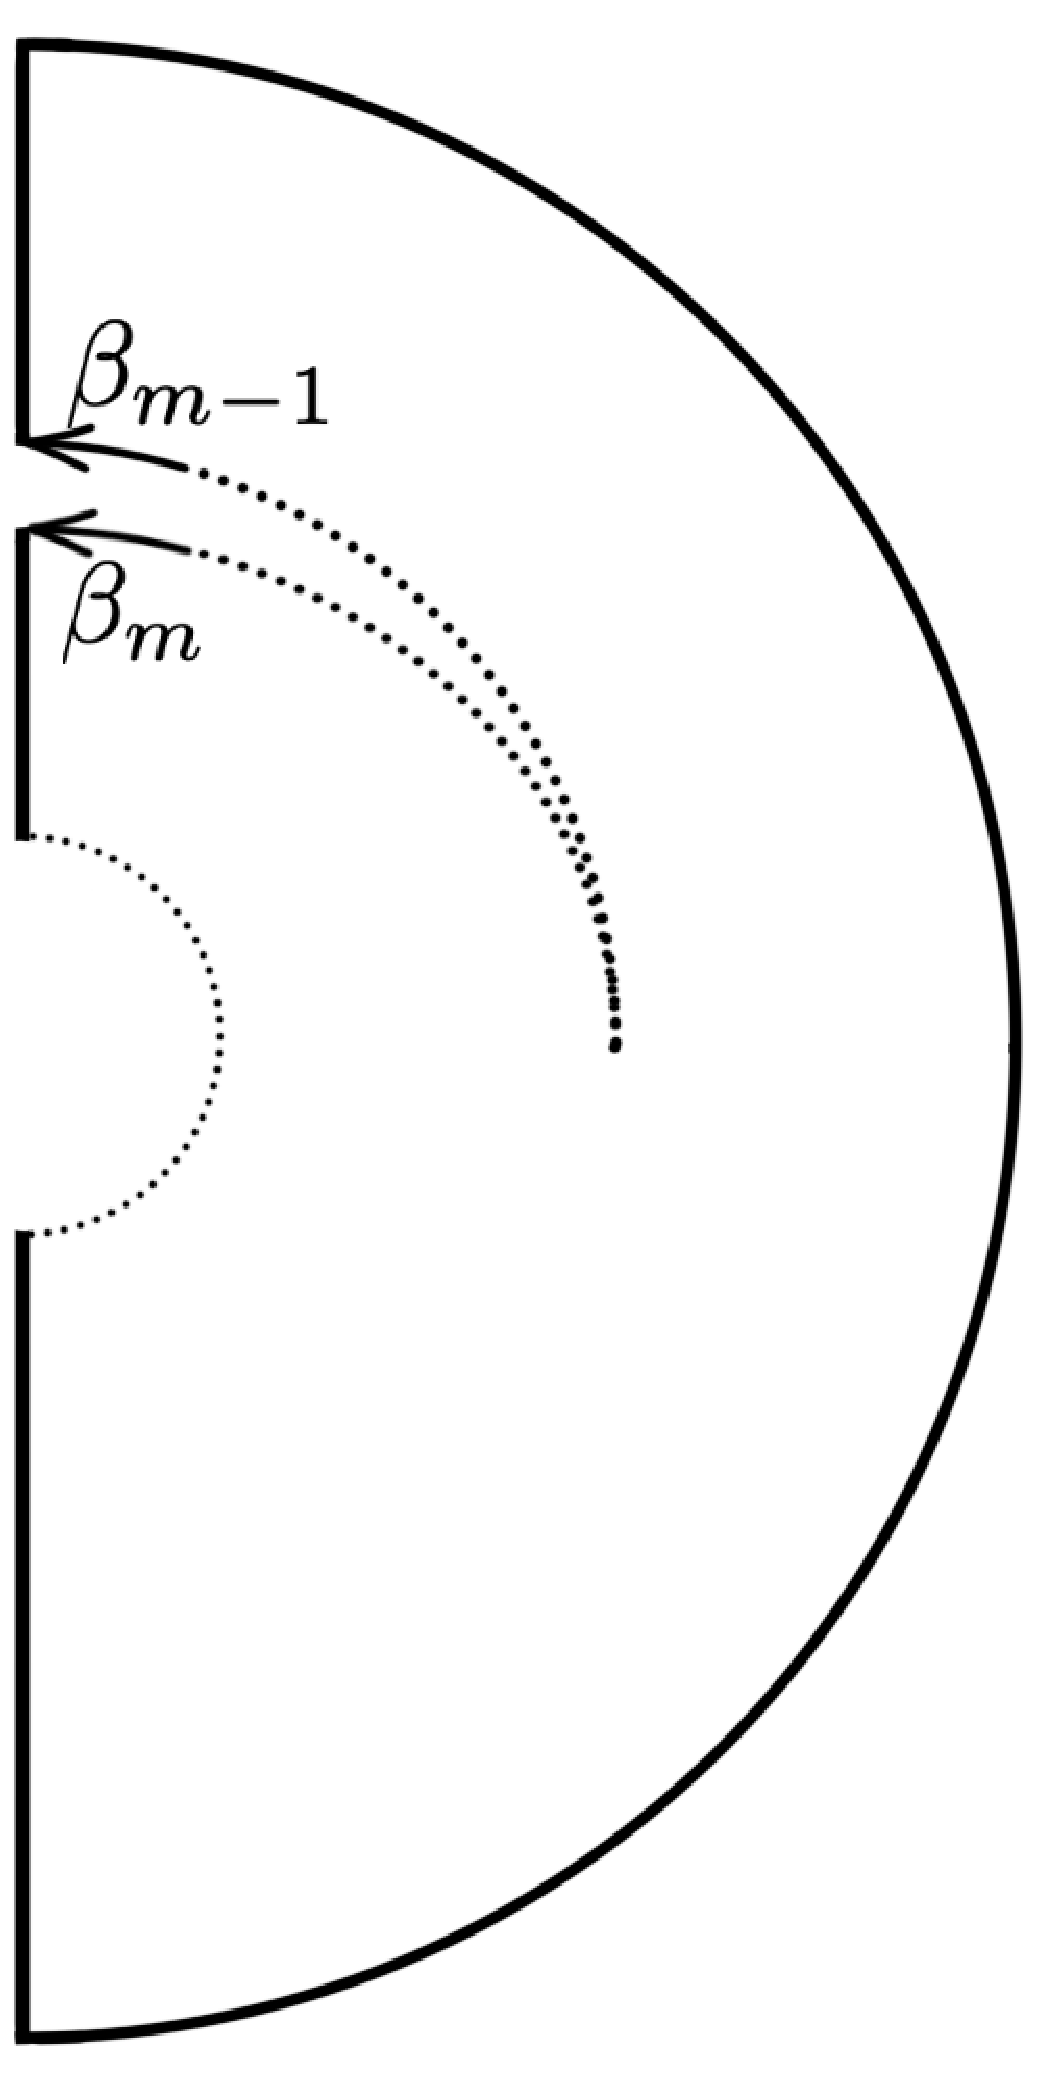
\includegraphics[width=2cm]{images/ch4/section3_circular/atoms/branching/branching_domain.pdf}
    \caption{\textbf{правее} $II_1$ и \textbf{левее} $\widehat{III}$.}
    \label{fig:pt10:_branching_domain}
\endminipage\hfill
\minipage{0.25\textwidth}
\centering
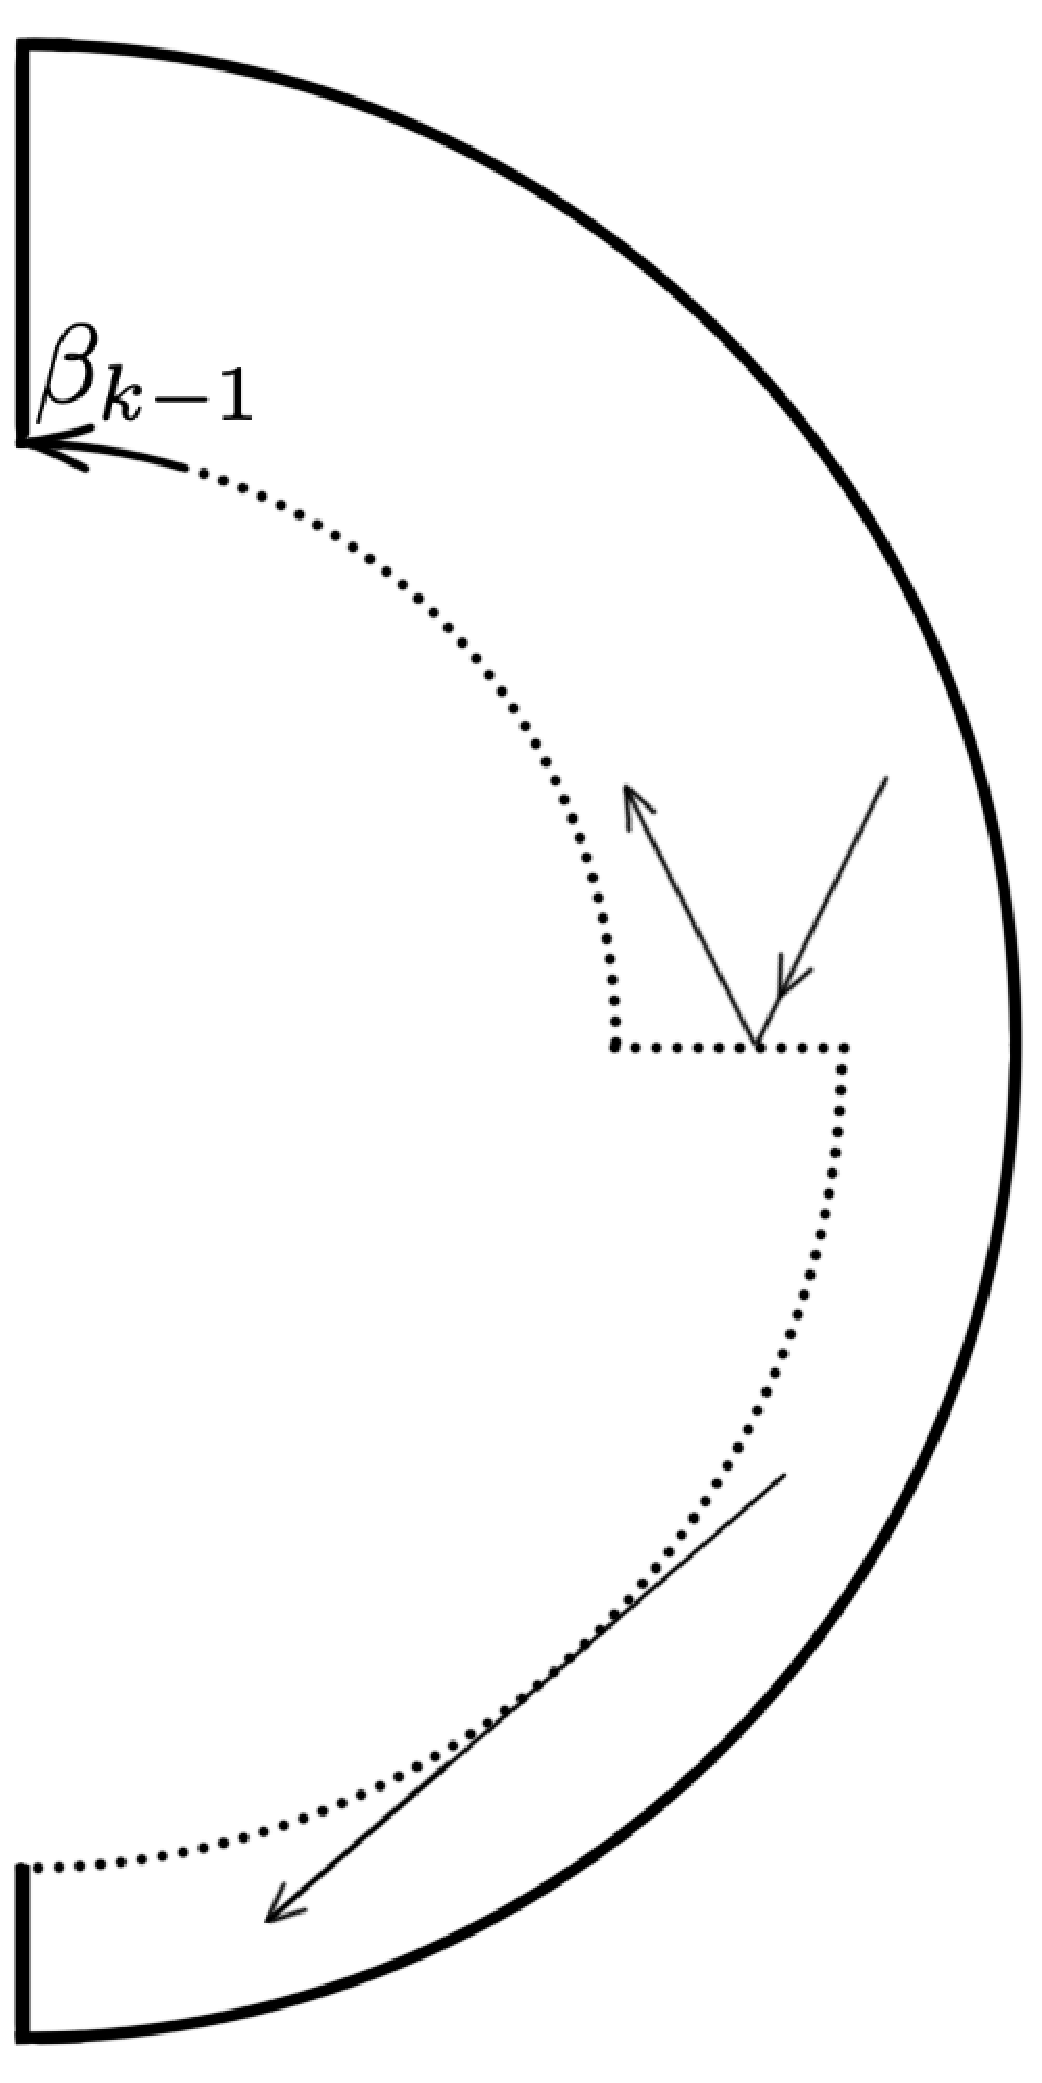
\includegraphics[width=2cm]{images/ch4/section3_circular/atoms/branching/terminal_max.pdf}
    \caption{\textbf{правее} $II_1, \widehat{III}$ и \textbf{левее} $IV_0$.}
    \label{fig:pt10:_terminal_max_domain}
\endminipage\hfill
\minipage{0.25\textwidth}
\centering
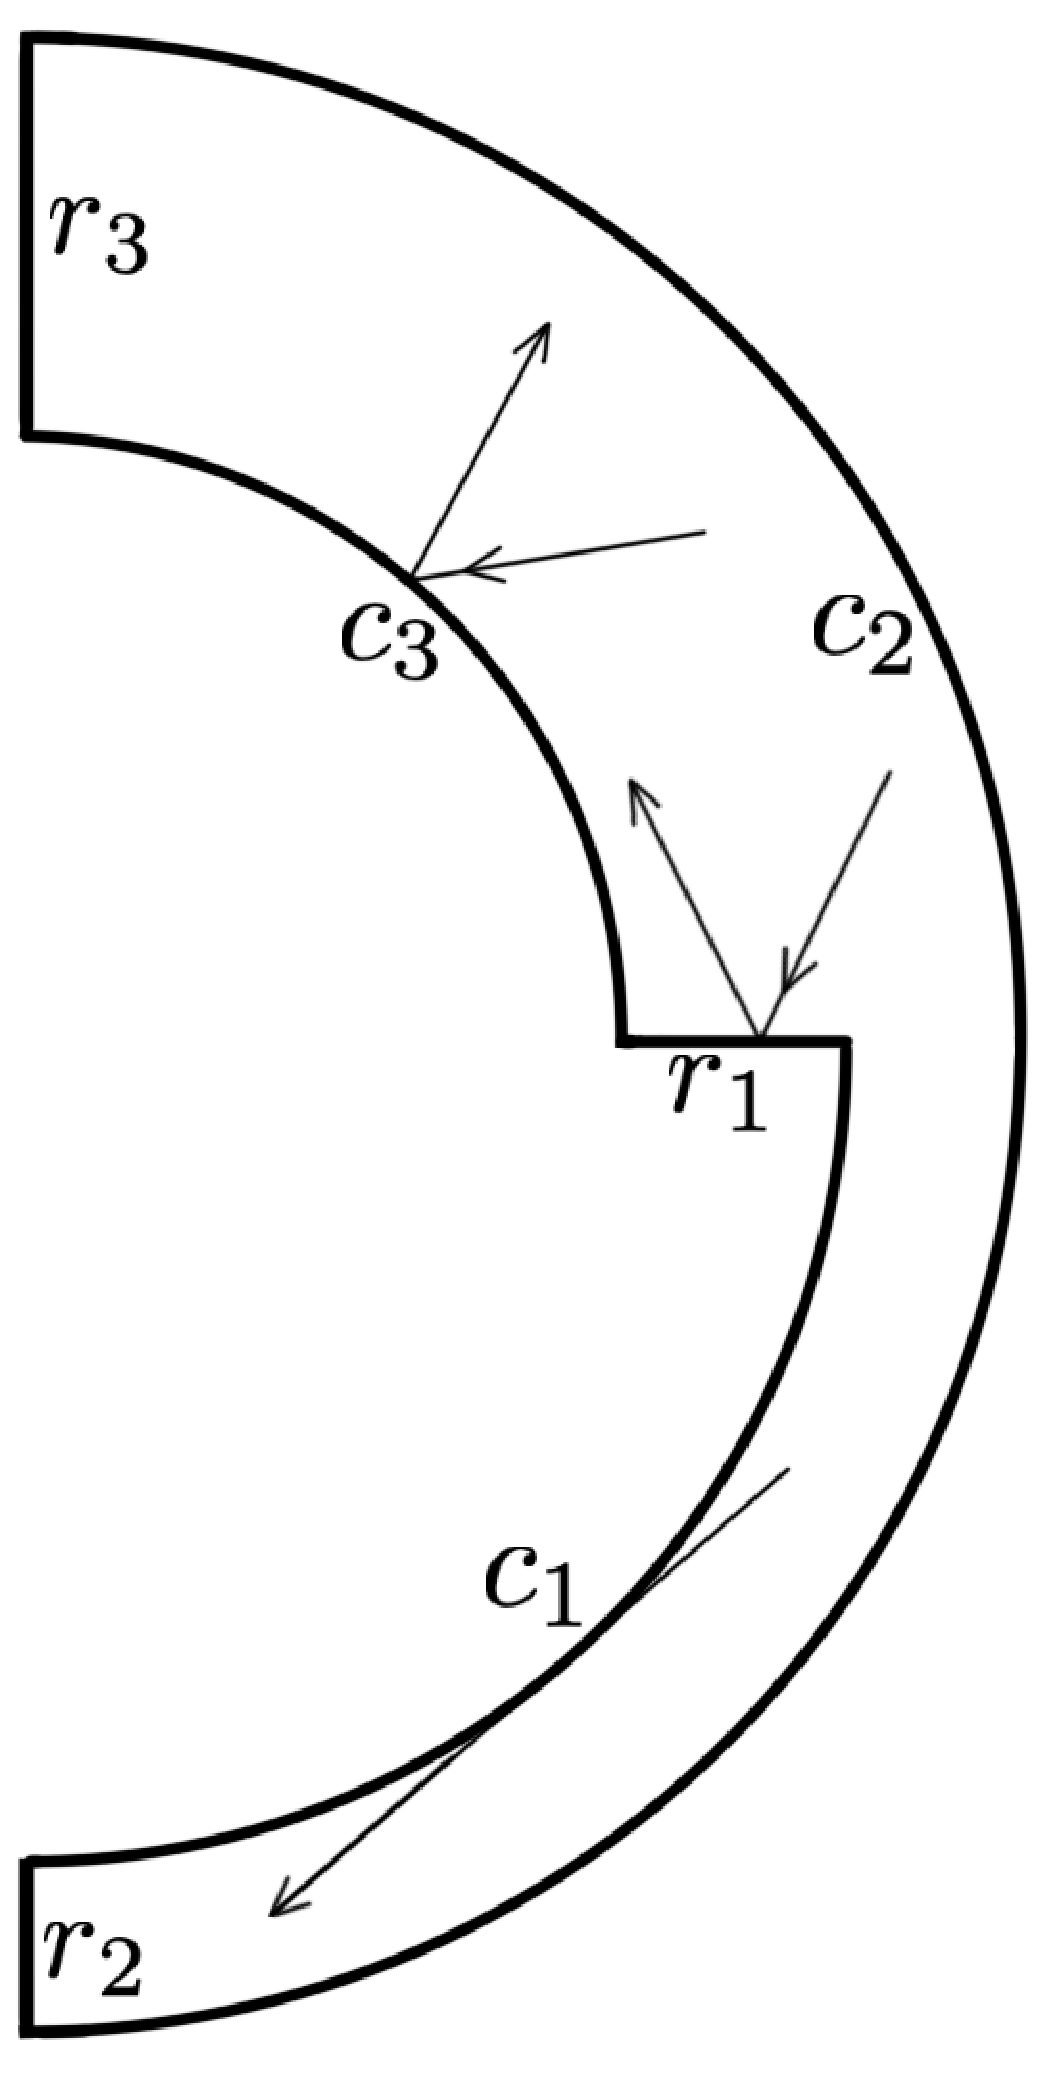
\includegraphics[width=2cm]{images/ch4/section3_circular/atoms/branching/sect3_C1_domain.pdf}
    \caption{\textbf{левее} $II_1, IV_0$, \textbf{правее} $\widehat{III}$.}
    \label{fig:pt10:_C1_domain}
\endminipage\hfill
\end{figure}

\begin{figure}[!htb]
\minipage{0.5\textwidth}
\centering
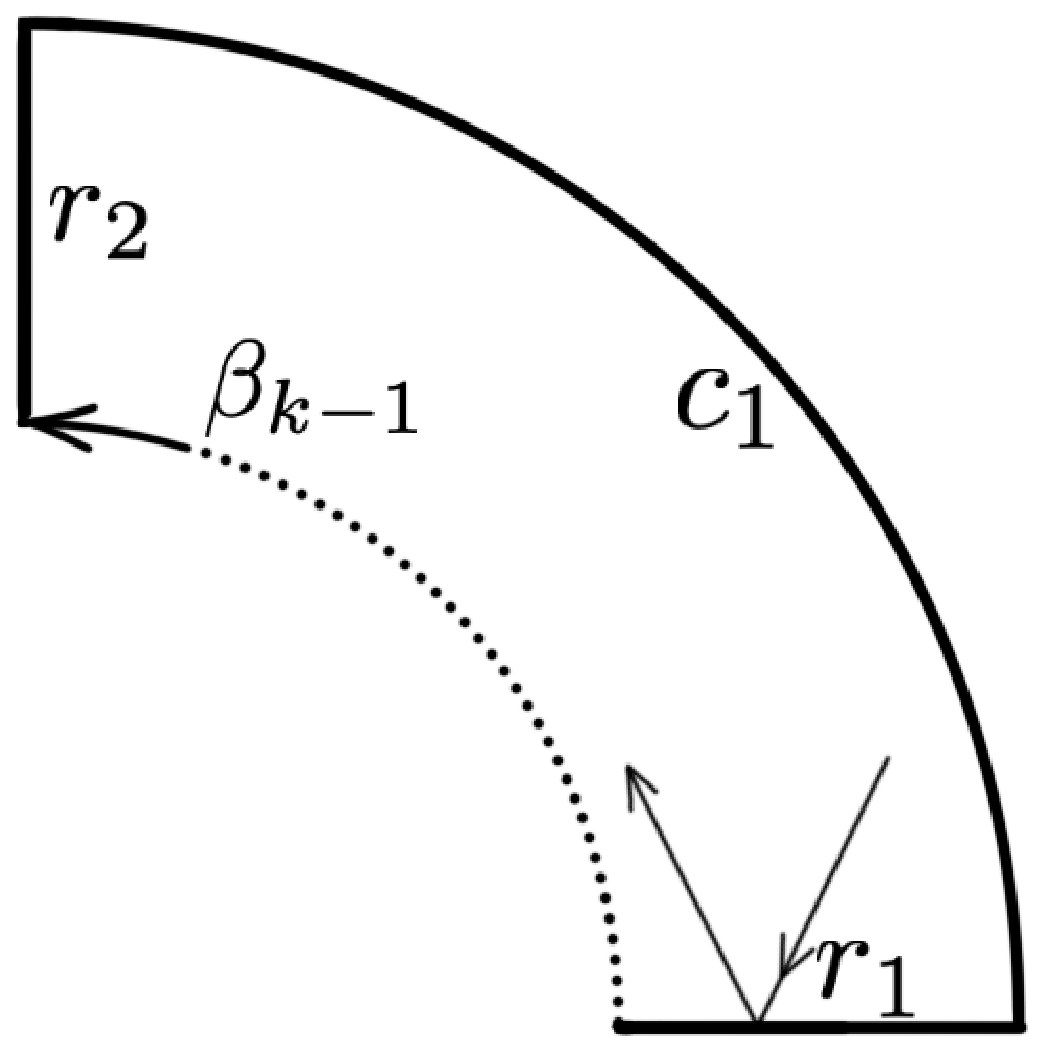
\includegraphics[width=2cm]{images/ch4/section3_circular/atoms/branching/B1Prime_max_domain.pdf}
    \caption{\textbf{правее} $II_1$ и $IV_0$.}
    \label{fig:pt10:_terminal_max_domain_B1Prime}
\endminipage\hfill
\minipage{0.5\textwidth}
\centering
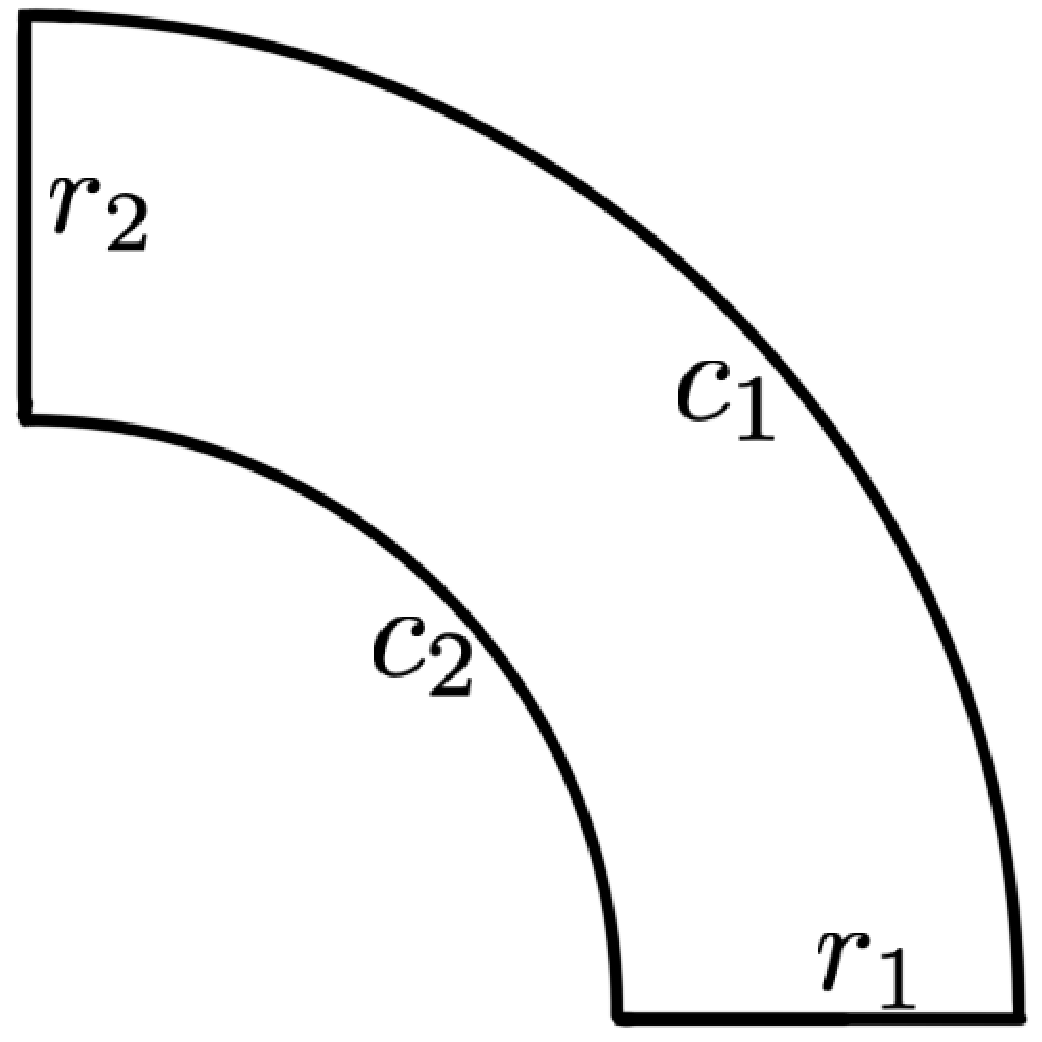
\includegraphics[width=2cm]{images/ch4/section3_circular/atoms/branching/sect3_C1_domain_prime.pdf}
    \caption{\textbf{левее} $II_1$ и  \textbf{правее} $IV_0$.}
    \label{fig:pt10:_C1_domainPrime}
\endminipage\hfill
\end{figure}
\label{st:stat_leaf_shapes}
\end{statement}


%Получается, если $\rho^2(\xi) \in C_k, k \geq 2$, то бильярдная траектория посещает $k$ листов $\Omega$, склеенных друг с другом по дуге $EF$. При этом два из этих листов допускают переход траектории через дугу $EF$ только в одном направлении (заметаемые бильярдной траекторией области изображены на рис. \ref{fig:pt10:_terminal_min_domain} и \ref{fig:pt10:_terminal_max_domain}), а $k-2$ листа, если они есть, допускают переходы в обоих направлениях (заметаемые области изображены на рис. \ref{fig:pt10:_branching_domain}).

\begin{remark}
Приведенные соображения справедливы для $n_1^2 < n_2^2$. Случай  $n_1^2 > n_2^2$ рассматривается аналогично: рассмотрим замену координат $(\widetilde{x}, \widetilde{y}) = \left( \frac{xy}{(y-x)r_1^2}, \frac{y}{y-x}\right)$. Тогда кривые $I_m$ будут задаваться уравнением $\widetilde{y} = m$, уравнения для $II_m$ --- уравнением $\widetilde{x} = m$, а для  $III_m$ примут вид $\widetilde{x} = m + \left\{\widetilde{y}\right\}$. Прямая $L$ снова будет горизонтальной прямой ($\widetilde{y} = \frac{n_1^2}{n_1^2-n_2^2}$). 
При пересечении дуги $EF$ интеграл $\Xi$ меняется таким образом, что точка на прямой $L$ сдвигается на вектор $\pm \gamma_L$, где $\gamma_L = (1,0)$. В свою очередь, прямая $y=\rho_2^2 = r_2^2$ соответствует прямой $\widetilde{y} = \widetilde{x} \frac{r_1^2}{r_2^2} + 1$. 

Тогда изображенные на  рис. \ref{fig:pt10:_B1_lattice_straight}---\ref{fig:pt10:_B1Prime_lattice} диаграммы справедливы и для $n_1^2 > n_2^2$. Но листы склейки на рис. 
 \ref{fig:pt10:_terminal_min_domain}--\ref{fig:pt10:_C1_domainPrime} будут выглядеть иначе.
\label{rem:diagram_reuse}
\end{remark}


\section{Неособые поверхности для случая $\left\{\xi < L_1\right\}$}\label{sec:ch5/sec6}
\subsection{Случай $n_1^2<n_2^2$}\label{sec:ch5/sec6/sub1}
На рис. \ref{fig:pt10:_B1Prime_lattice} отрезок $IV_0$ в $(\widetilde{x}, \widetilde{y})$
пересекает по одной области, относящейся к классам $C_1, \ldots, C_k, C_{k+1}$, где $k = \left \lfloor \frac{r_2^2}{r_2^2 - r_1^2} \right \rfloor$. 
Для каждой области  $C_i$, пересеченной отрезком $IV_0$ выделим ту часть, что находится по правую часть от $IV_0$  в отдельный класс $C_i'$.
Определим отрезки прямых 
\begin{equation}
IV_m =  \left\{ \widetilde{y} = (\widetilde{x} + m) \frac{r_1^2}{r_2^2} + 1 \right\} \cap \left\{\widetilde{y}< \frac{r_2^2}{r_2^2-r_1^2}\right\}.
\label{eq:IVdef}
\end{equation} 
Отрезки $IV_m, m \leq k$, пересекают множества типа $C_2, \ldots, C_k, C_{k+1}$. По аналогии с $IV_0$ из пересеченных множеств выделим множества  $C_2', \ldots, C_k'$ (см. пример на рис. \ref{fig:pt10:_C_kPrime_definitions}).

%соответствующий координатной линии $\rho_1^2 = r_2^2$, проходит через несколько множеств $C_m$. Для удобства формулировки следующего утверждения выделим из $C_m$ классы $C_m'$, лежащие под указанной прямой $IV_0$ или ее сдвинутыми копиями $IV_m, m>0$, то есть в закрашенной серым области на рис. \ref{fig:pt10:_C_kPrime_definitions}.
\begin{figure}[!htb]
\centering
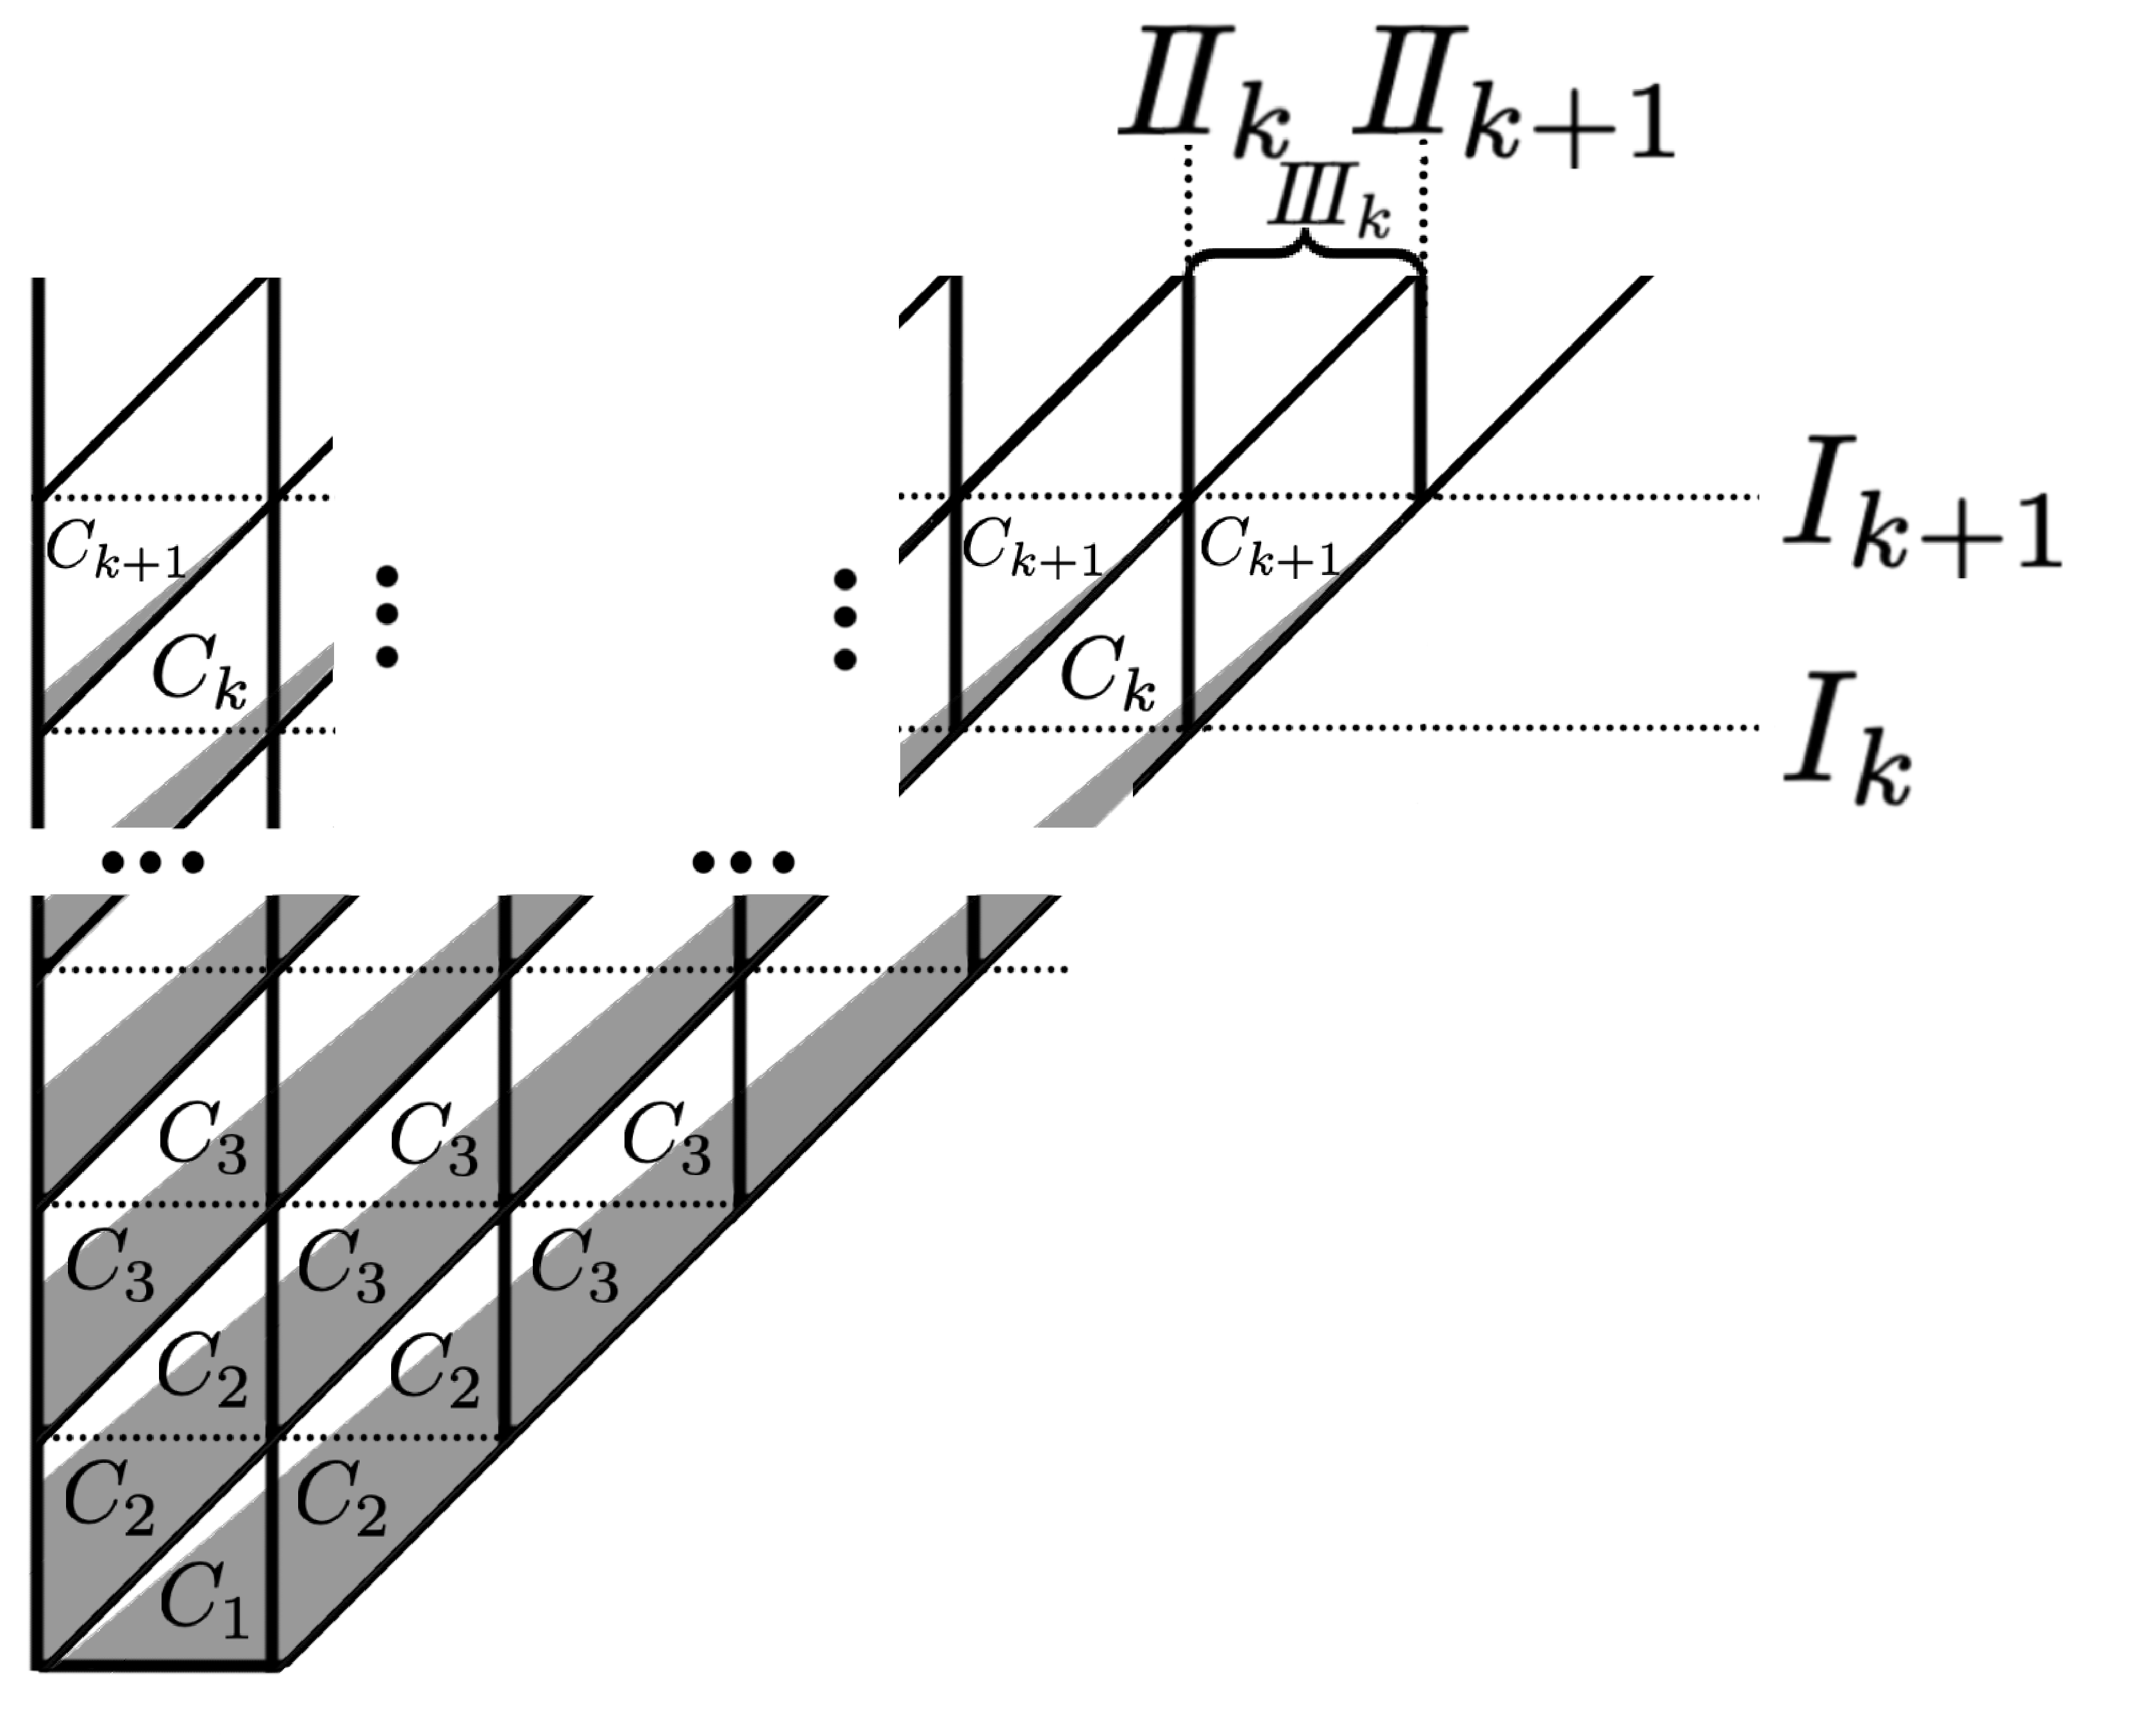
\includegraphics[width=7cm]{images/ch4/section3_circular/atoms/branching/C_kPrime_definitions.pdf}
    \caption{Область $C_m'$ --- это часть $C_m$; область $C_m'$ выделена серым.}
    \label{fig:pt10:_C_kPrime_definitions}
\end{figure}

\begin{remark}
Классы $C_k'$ не определены при $k > \left\lfloor \frac{r_2^2}{r_2^2-r_1^2} \right\rfloor$, поскольку отрезки прямых $IV_k$ не пересекают области, относящиеся к таким $C_k$.
\end{remark}

Напомним, что при $\Xi$ таком, что $P(\Xi) \in \{\xi < L_1\}$, бильярдные траектории разбиваются на фрагменты $T_m, m \geq 1$, точками пересечения с дугой $EF$. При этом  каждому фрагменту  $T_m$ сопоставляется одна из уникальных точек $P(\Xi_1), \ldots, P(\Xi_k)$, соответствующих возможным значениям интеграла $\Xi$ (напомним: он многозначен). В свою очередь, каждая из точек $P(\Xi_j)$ соответствует одной из поверхностей с краем и может быть определена как изоинтегральная поверхность $\Xi = \Xi_j$.

Попарно поверхности с краем $\{\Xi = \Xi_m\}$ и $\{\Xi = \Xi_{m+1}\}$, $m=1, \ldots, k-1$ отождествляются по дуге, которую мы обозначим $\beta_m$. При проекции $\pi$ все дуги $\beta_1, \ldots, \beta_{k-1}$ отображаются в дугу $EF$.

Таким образом, соответствующая бильярдной траектории кривая расположена на склейке поверхностей $\{\Xi = \Xi_m\}, m=1,\ldots, k$.
Формально эту поверхность можно определить как 
$$S_\Xi = \left\{\Xi - \varkappa = 0 \mod \gamma  \ | \ \varkappa : P(\varkappa) \in \{\xi<L_1\} \right\}.$$

\begin{theorem}
В области $\left\{\xi < L_1\right\}$ поверхности $S_\Xi$ являются сферами с $2m$ ручками, если $P(\Xi) \in C_m$ и сферами с $2m-1$ ручками, если $P(\Xi) \in C_m'$ и $m \leq \left\lfloor \frac{r_2^2}{r_2^2-r_1^2} \right\rfloor$. 
\label{th:pt10:th1}
\end{theorem}


%\textcolor{red}{===Этот текст мне не очень нравится===}

\begin{proof}
Для точек бильярдной траектории $(x, y, v_x, v_y)$ изоэнергитического многообразия определим проекцию на заметаемую область в $\Omega$ по формуле
$$\pi : (x, y, v_x, v_y) \mapsto (x,y).$$

Поверхность $S_\Xi$ разбивается на несколько частей $\{\Xi = \Xi_m\}, m = 1 \ldots, k$, по дугам, которые проекция $\pi$ отображает на дугу $EF$. 
%На каждом фрагменте $\Xi = \Xi_m$ поверхности содержится 
%кривая в $Q^3$, соответствующая всем  фрагментам бильярдной траектории $T_k$, продолжения звеньев которых касаются окружности радиуса $\rho_1$ в области $\Omega_1$ и радиуса $\rho_2$ --- в области $\Omega_2$, где радиусы окружностей получаются как $P(\Xi_m) = (\rho_1^2, \rho_2^2)$.

Часть $\Xi = \Xi_m$ поверхности $S_\Xi$ при проекции $\pi$ покрывает собой образ $(\Omega_1 \setminus B_{\rho_1}) \cup (\Omega_2 \setminus B_{\rho_2}) \setminus EF = \widetilde{\Omega}_m$, где $B_r$ обозначает диск радиуса $r$ с радиусом в нуле. При этом в каждой внутренней точке образа покрытие четырехлистно.

Следовательно, в прообразе  $\widetilde{\Omega}_m$ при отображении $\pi$ можно выбрать на поверхности $\Xi = \Xi_m$ по 4 прообраза для областей, проектирующихся в $\Omega_1 \setminus B_{\rho_1}$ и $\Omega_2 \setminus B_{\rho_2}$. Обозначим  эти прообразы как $\Omega_{1, j}$ и $\Omega_{2,j}, j=1, \ldots, 4$, где нумерация определена по следующему правилу:
\begin{equation}
\begin{array}{ll}
1: & \text{ вектор } (v_x, v_y) \text{ направлен по часовой стрелке к каустике}, \\
2: & \text{ вектор } (v_x, v_y) \text{ направлен против часовой стрелки к каустике}, \\
3: & \text{ вектор } (v_x, v_y) \text{ направлен против часовой стрелки от каустики}, \\
4: & \text{ вектор } (v_x, v_y) \text{ направлен по часовой стрелке от каустики}.
\end{array}
\label{eq:foc_numeration_circle}
\end{equation}
Проследим правила склейки:

$\bullet$ Области $\Omega_{1, j}, \Omega_{2, j}$ отождествляются по общей границе, которая проектируется в отрезок $FG$, поскольку правила $(\ast)$ сохраняют номер в случае, когда обе каустики являются окружностями. Нумерация соседствующих через дугу $EF$ областей также сохраняется.

$\bullet$ В силу стандартного закона отражения области $\Omega_{1, 1}$ приклеиваются к областям $\Omega_{1,4}$ на дугах окружностей, аналогично $\Omega_{1,2}$ подклеивается к области $\Omega_{1,3}$. Аналогичное правило справедливо для областей $\Omega_{2,1}, \Omega_{2,2}, \Omega_{2,3}, \Omega_{2,4}$. Для краткости обозначим это отождествление $(1 \sim 4, 2 \sim 3)$.

$\bullet$ Описанное выше правило склейки возникает на дугах каустик в силу совпадания векторов.

$\bullet$ В силу стандартного закона отражения области $\Omega_{1, 1}$ приклеиваются к областям $\Omega_{1,2}$ на проходящих через центр окружности прямых, то же справедливо для $\Omega_{1,3}$ и $\Omega_{1,4}$. Аналогичное правило справедливо для областей $\Omega_{2,1}, \Omega_{2,2}, \Omega_{2,3}, \Omega_{2,4}$. Для краткости обозначим это отождествление $(1 \sim 2, 3 \sim 4)$.
\begin{equation}
c = (1 \sim 4, 2 \sim 3), \ r = (1 \sim 2, 3 \sim 4)
\label{eq:RCrules_circle} 
\end{equation}


\textit{Случай $C_k$, где $k\geq2$}. 

Как следует из утверждения \ref{st:stat_leaf_shapes}, 
поверхность $S_\Xi$ получается склейкой нескольких листов, 
а именно:

$\bullet$ одного листа, соответствующего точке $Q$ \textbf{левее} $II_1$ и \textbf{левее} $\widehat{III}$

$\bullet$ одного листа, соответствующего точке $Q$ \textbf{правее} $II_1, \widehat{III}$ и \textbf{левее} $IV_0$.

$\bullet$ и $k-2$ листов, каждый из которых соответствует точкам $Q$ \textbf{правее} $II_1$ и \textbf{левее} $\widehat{III}$.

Эти листы склейки (см. рис.  \ref{fig:pt10:_terminal_min_domain}--\ref{fig:pt10:_terminal_max_domain}) требуется склеить по дугам $\beta_m, m=1, \ldots, k-1$.
На рис. \ref{fig:pt10:_terminal_min_domain_transformed}--\ref{fig:pt10:_terminal_max_domain_transformed} листы деформированы для наглядности.
\begin{figure}[!htb]
\minipage{0.33\textwidth}
\centering
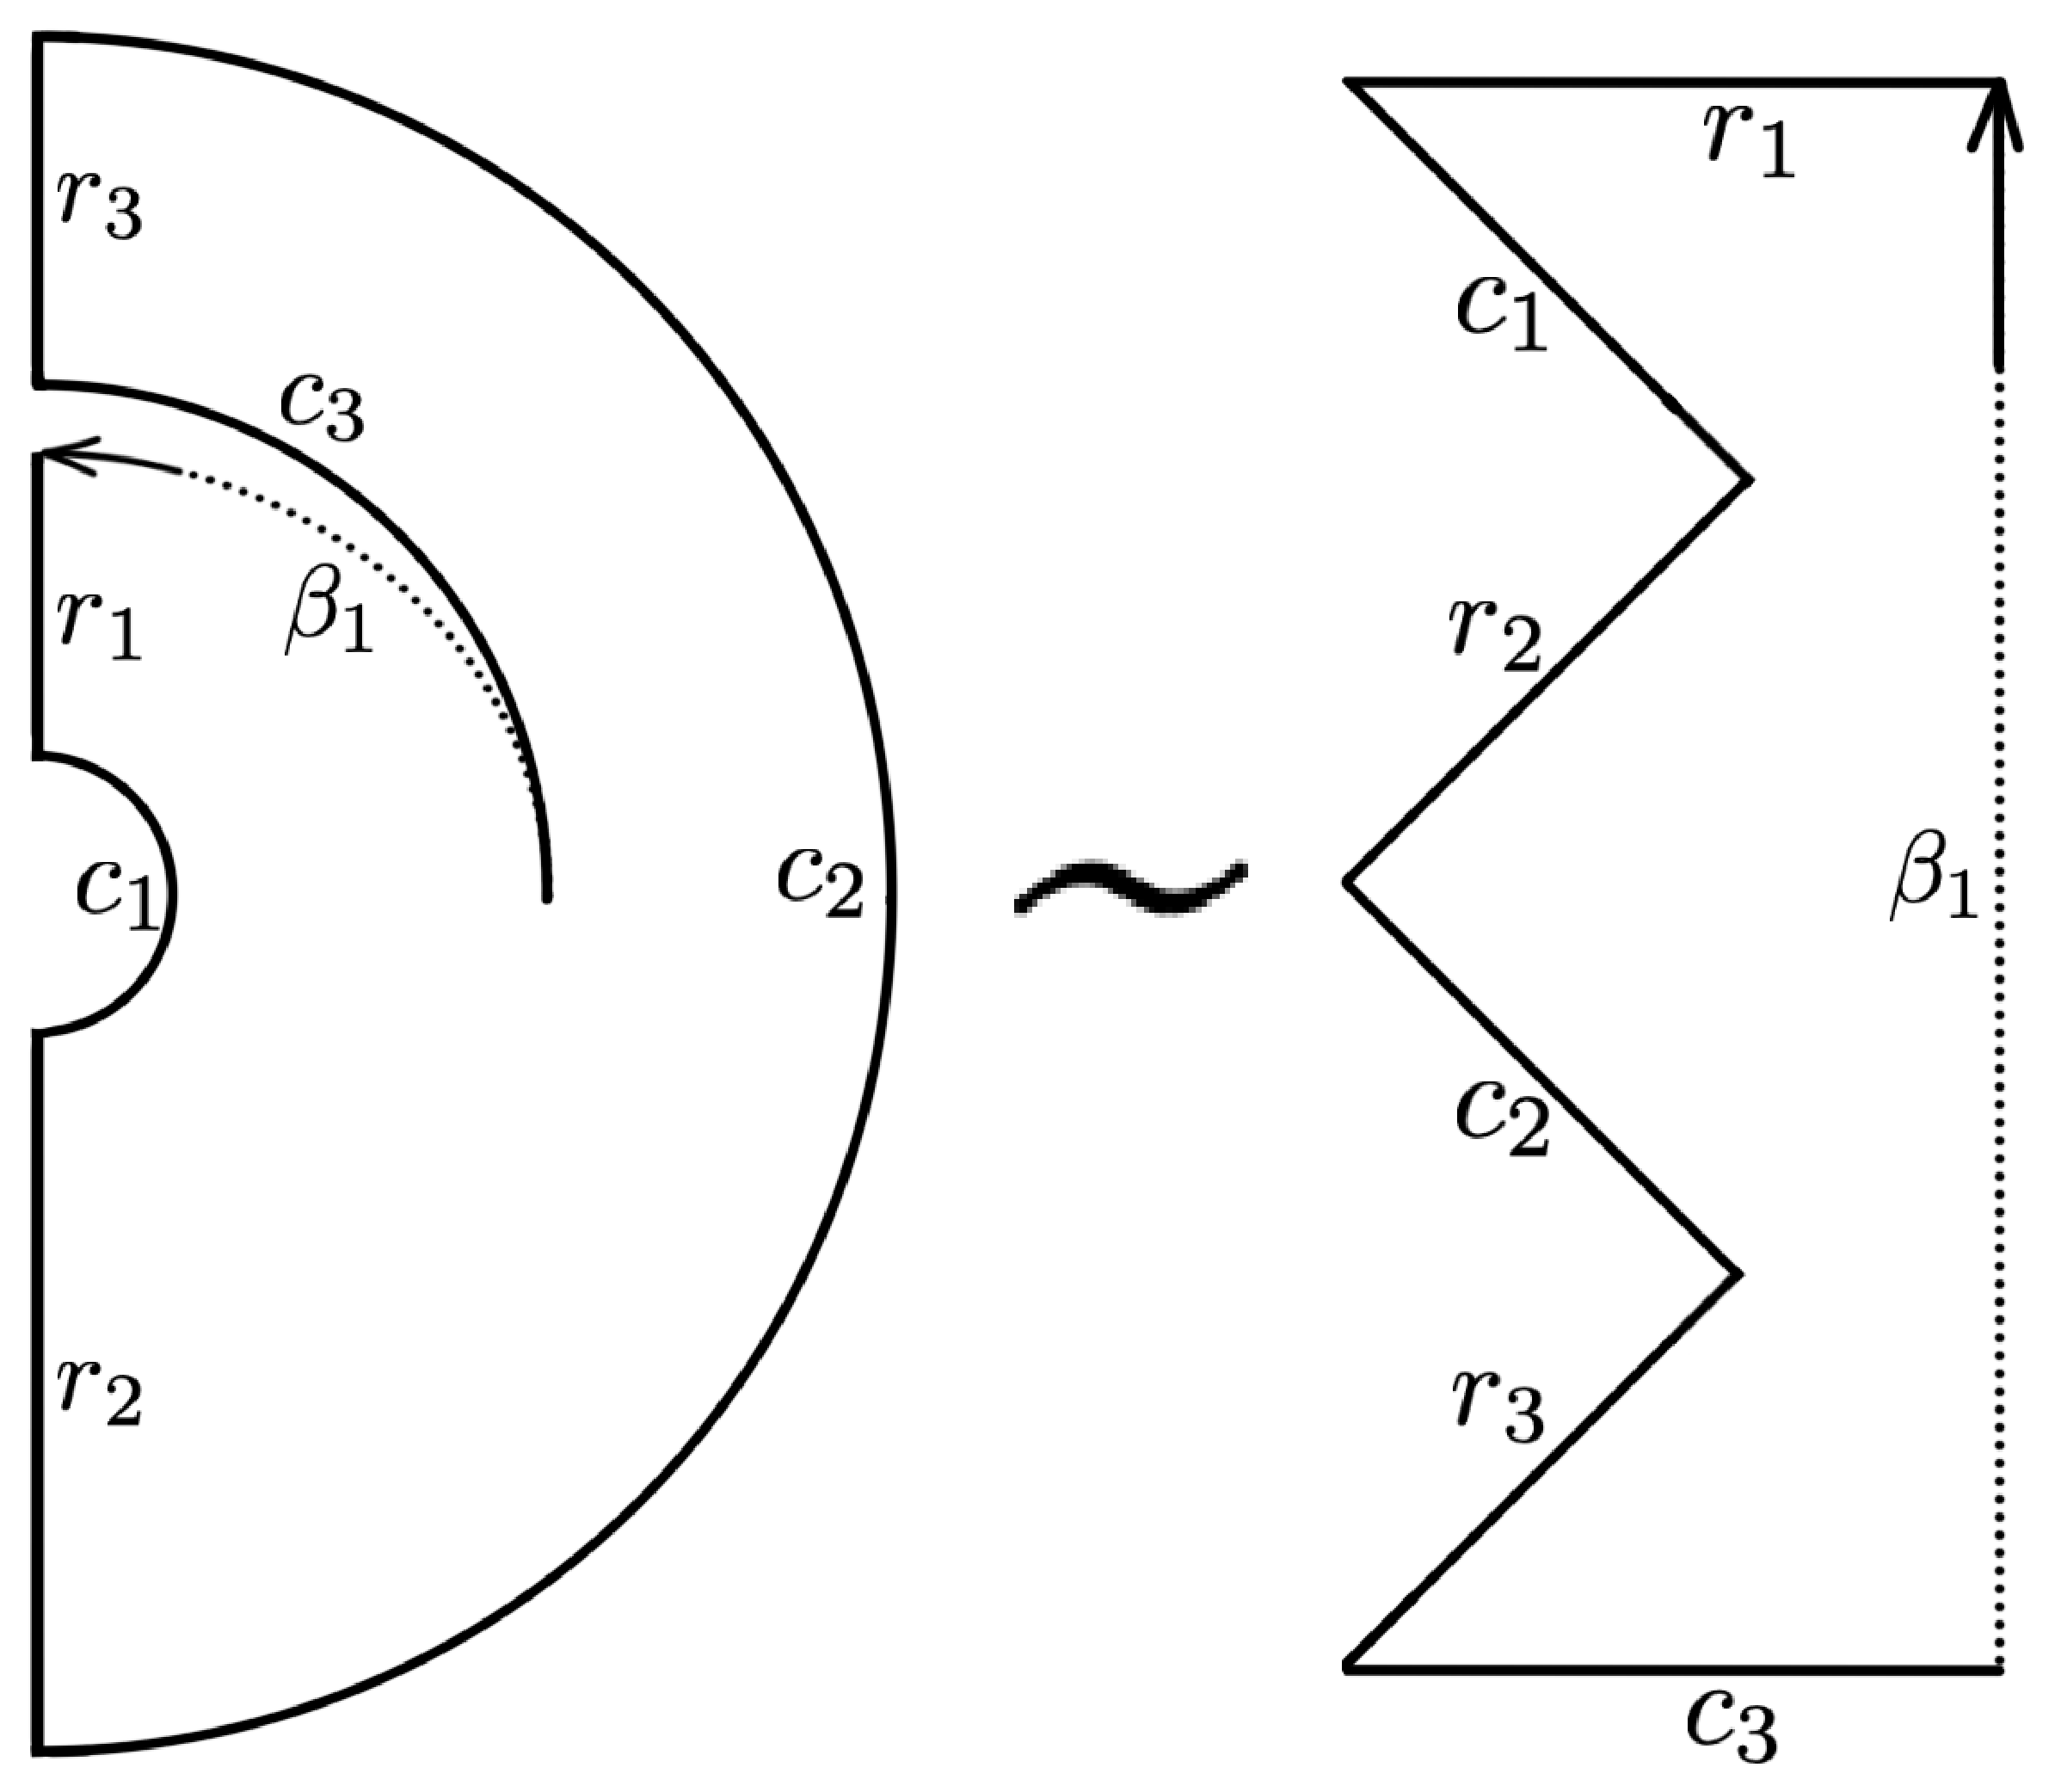
\includegraphics[scale=0.1]{images/ch4/section3_circular/atoms/branching/terminal_min_transformed.pdf}
%\caption{Преобразование рис. \ref{fig:pt10:_terminal_min_domain}}
\caption{}
    \label{fig:pt10:_terminal_min_domain_transformed}
\endminipage\hfill
\minipage{0.33\textwidth}
\centering
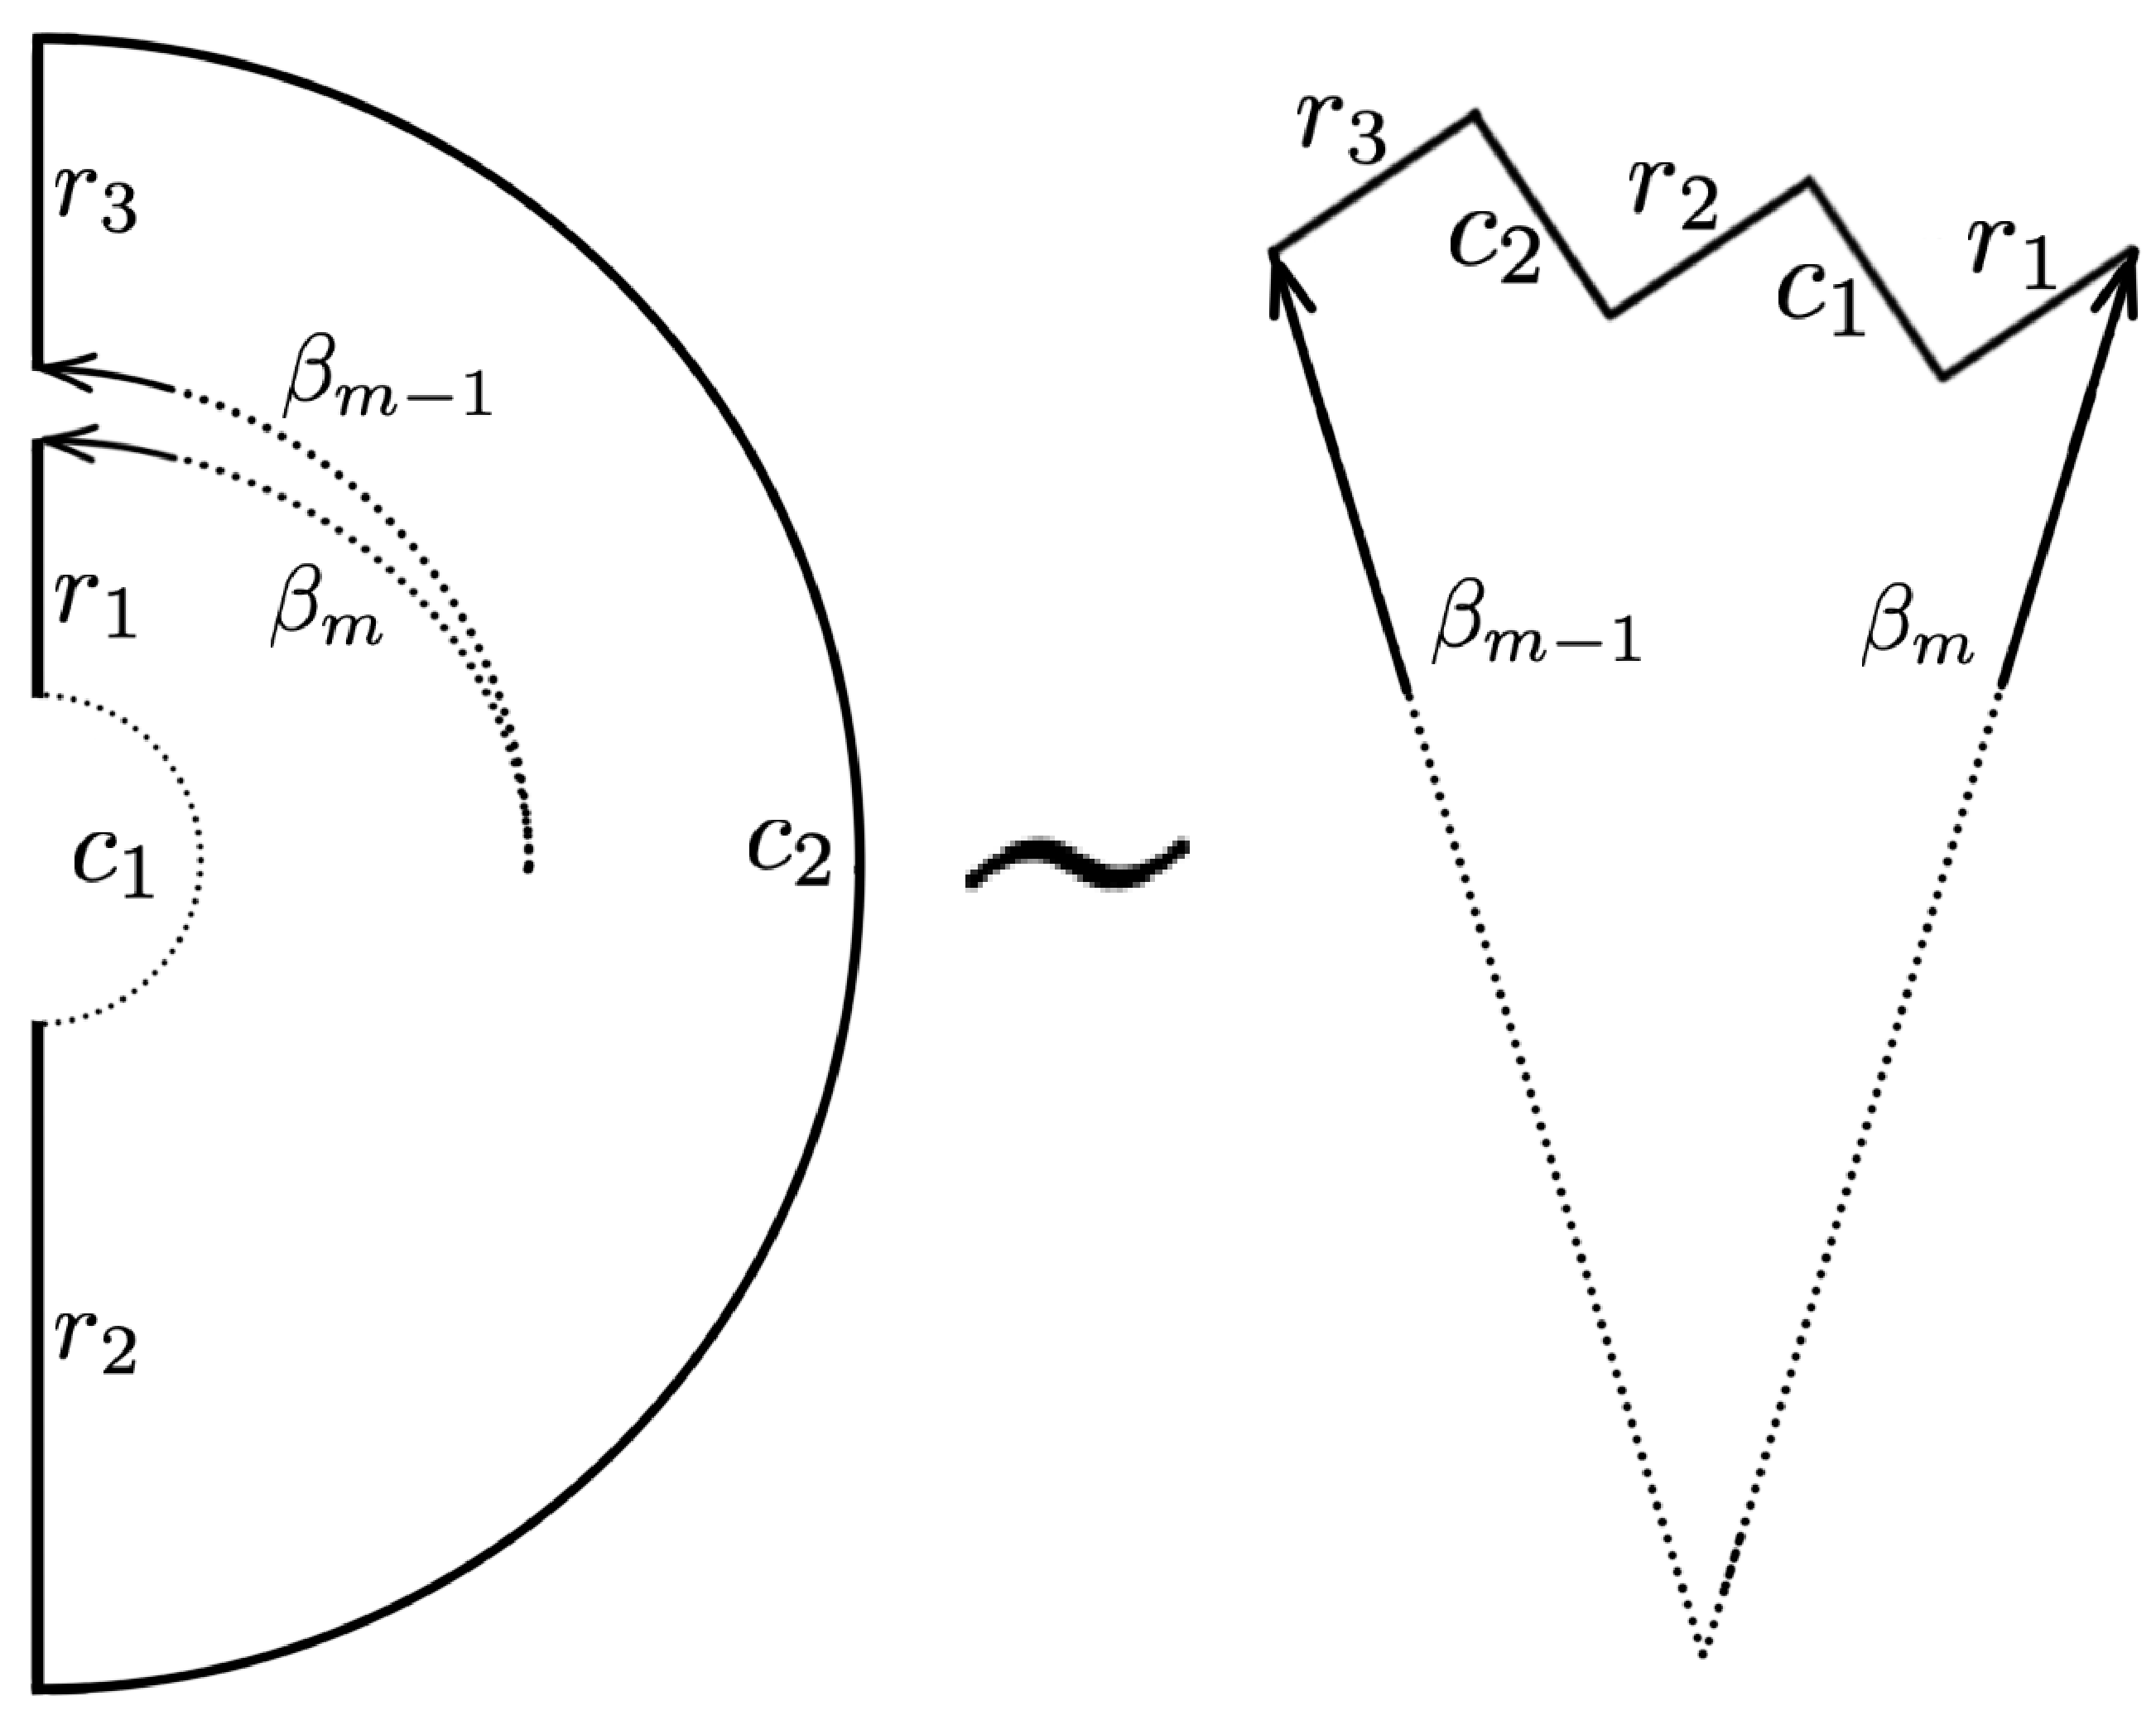
\includegraphics[scale=0.1]{images/ch4/section3_circular/atoms/branching/branching_domain_transformed.pdf}
%    \caption{Преобразование рис. \ref{fig:pt10:_branching_domain}}
\caption{}
    \label{fig:pt10:_branching_domain_transformed}
\endminipage\hfill
\minipage{0.33\textwidth}
\centering
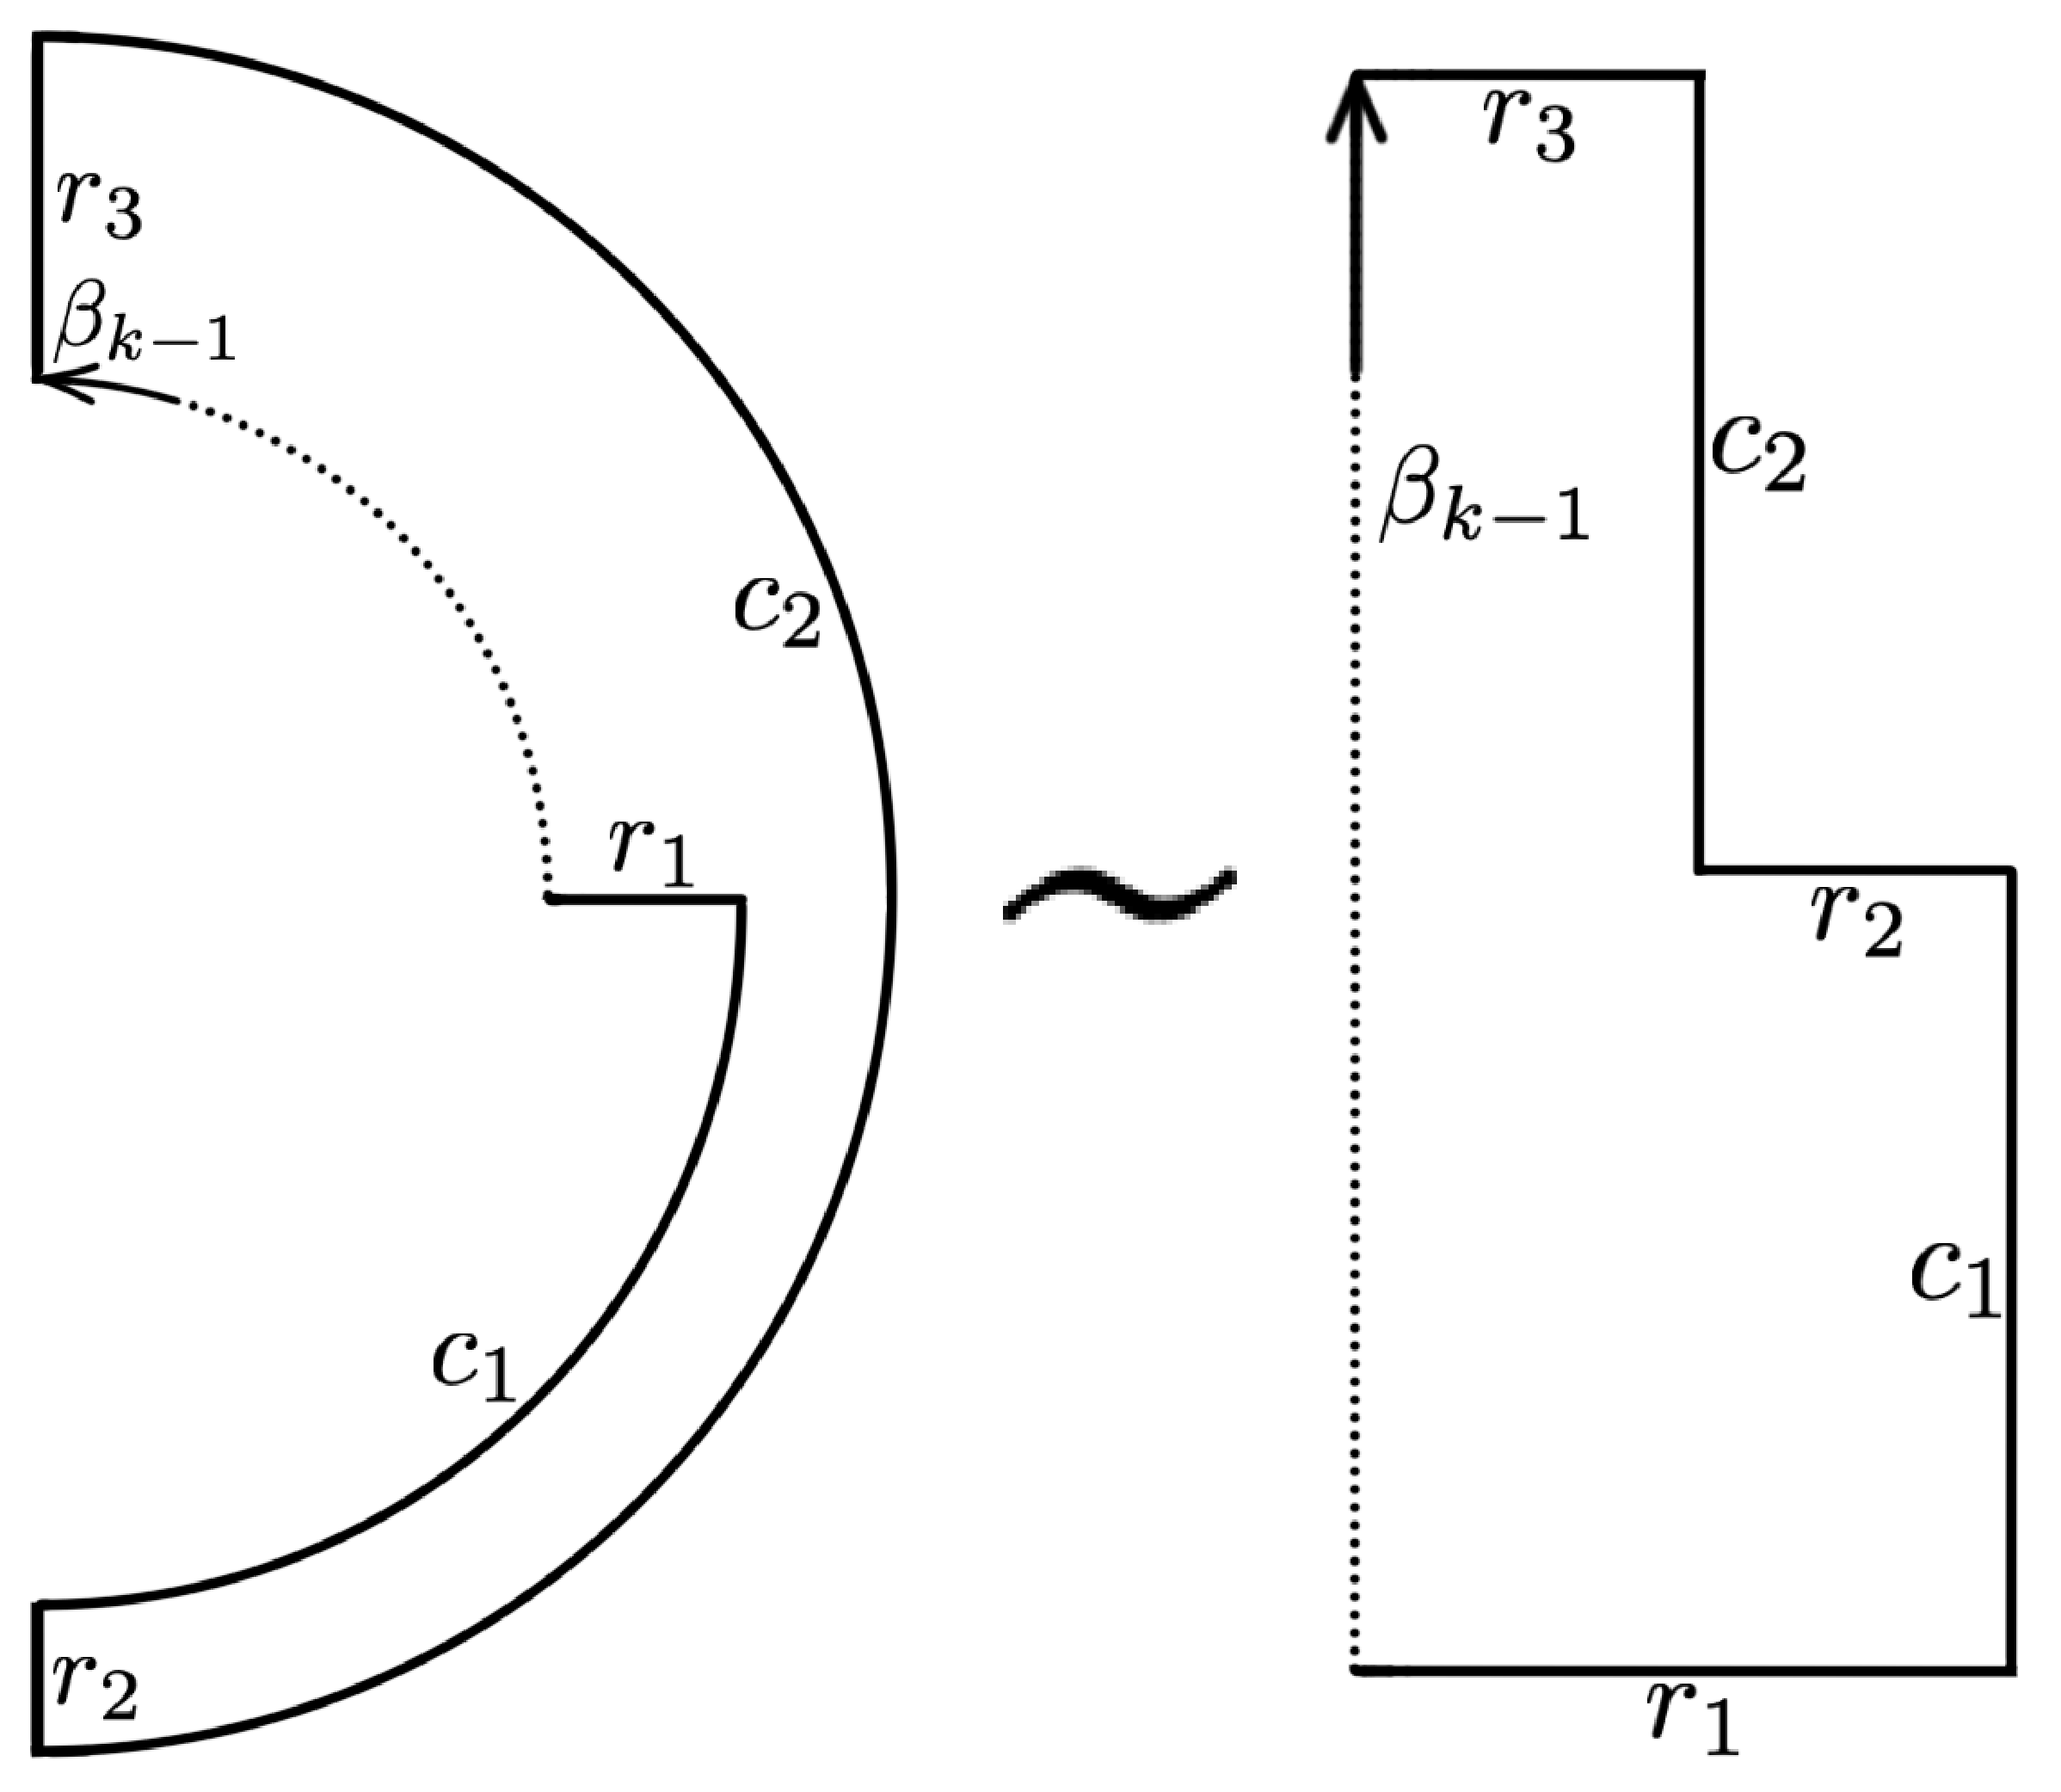
\includegraphics[scale=0.1]{images/ch4/section3_circular/atoms/branching/terminal_max_transformed.pdf}
%    \caption{Преобразование рис. \ref{fig:pt10:_terminal_max_domain}}
\caption{}
    \label{fig:pt10:_terminal_max_domain_transformed}
\endminipage\hfill

\medskip


\centering
Представление областей с рис. \ref{fig:pt10:_terminal_min_domain}---\ref{fig:pt10:_terminal_max_domain} в виде многоугольников.
%    \label{fig:pt10:_domains_transformed}
\end{figure}

Результат склейки $\widetilde{\Omega}$ листов вдоль дуг $\beta_1, \ldots, \beta_{k-1}$ показан на рис.    \ref{fig:pt10:_big_domain_transformed}.
\begin{figure}[!htb]
\centering
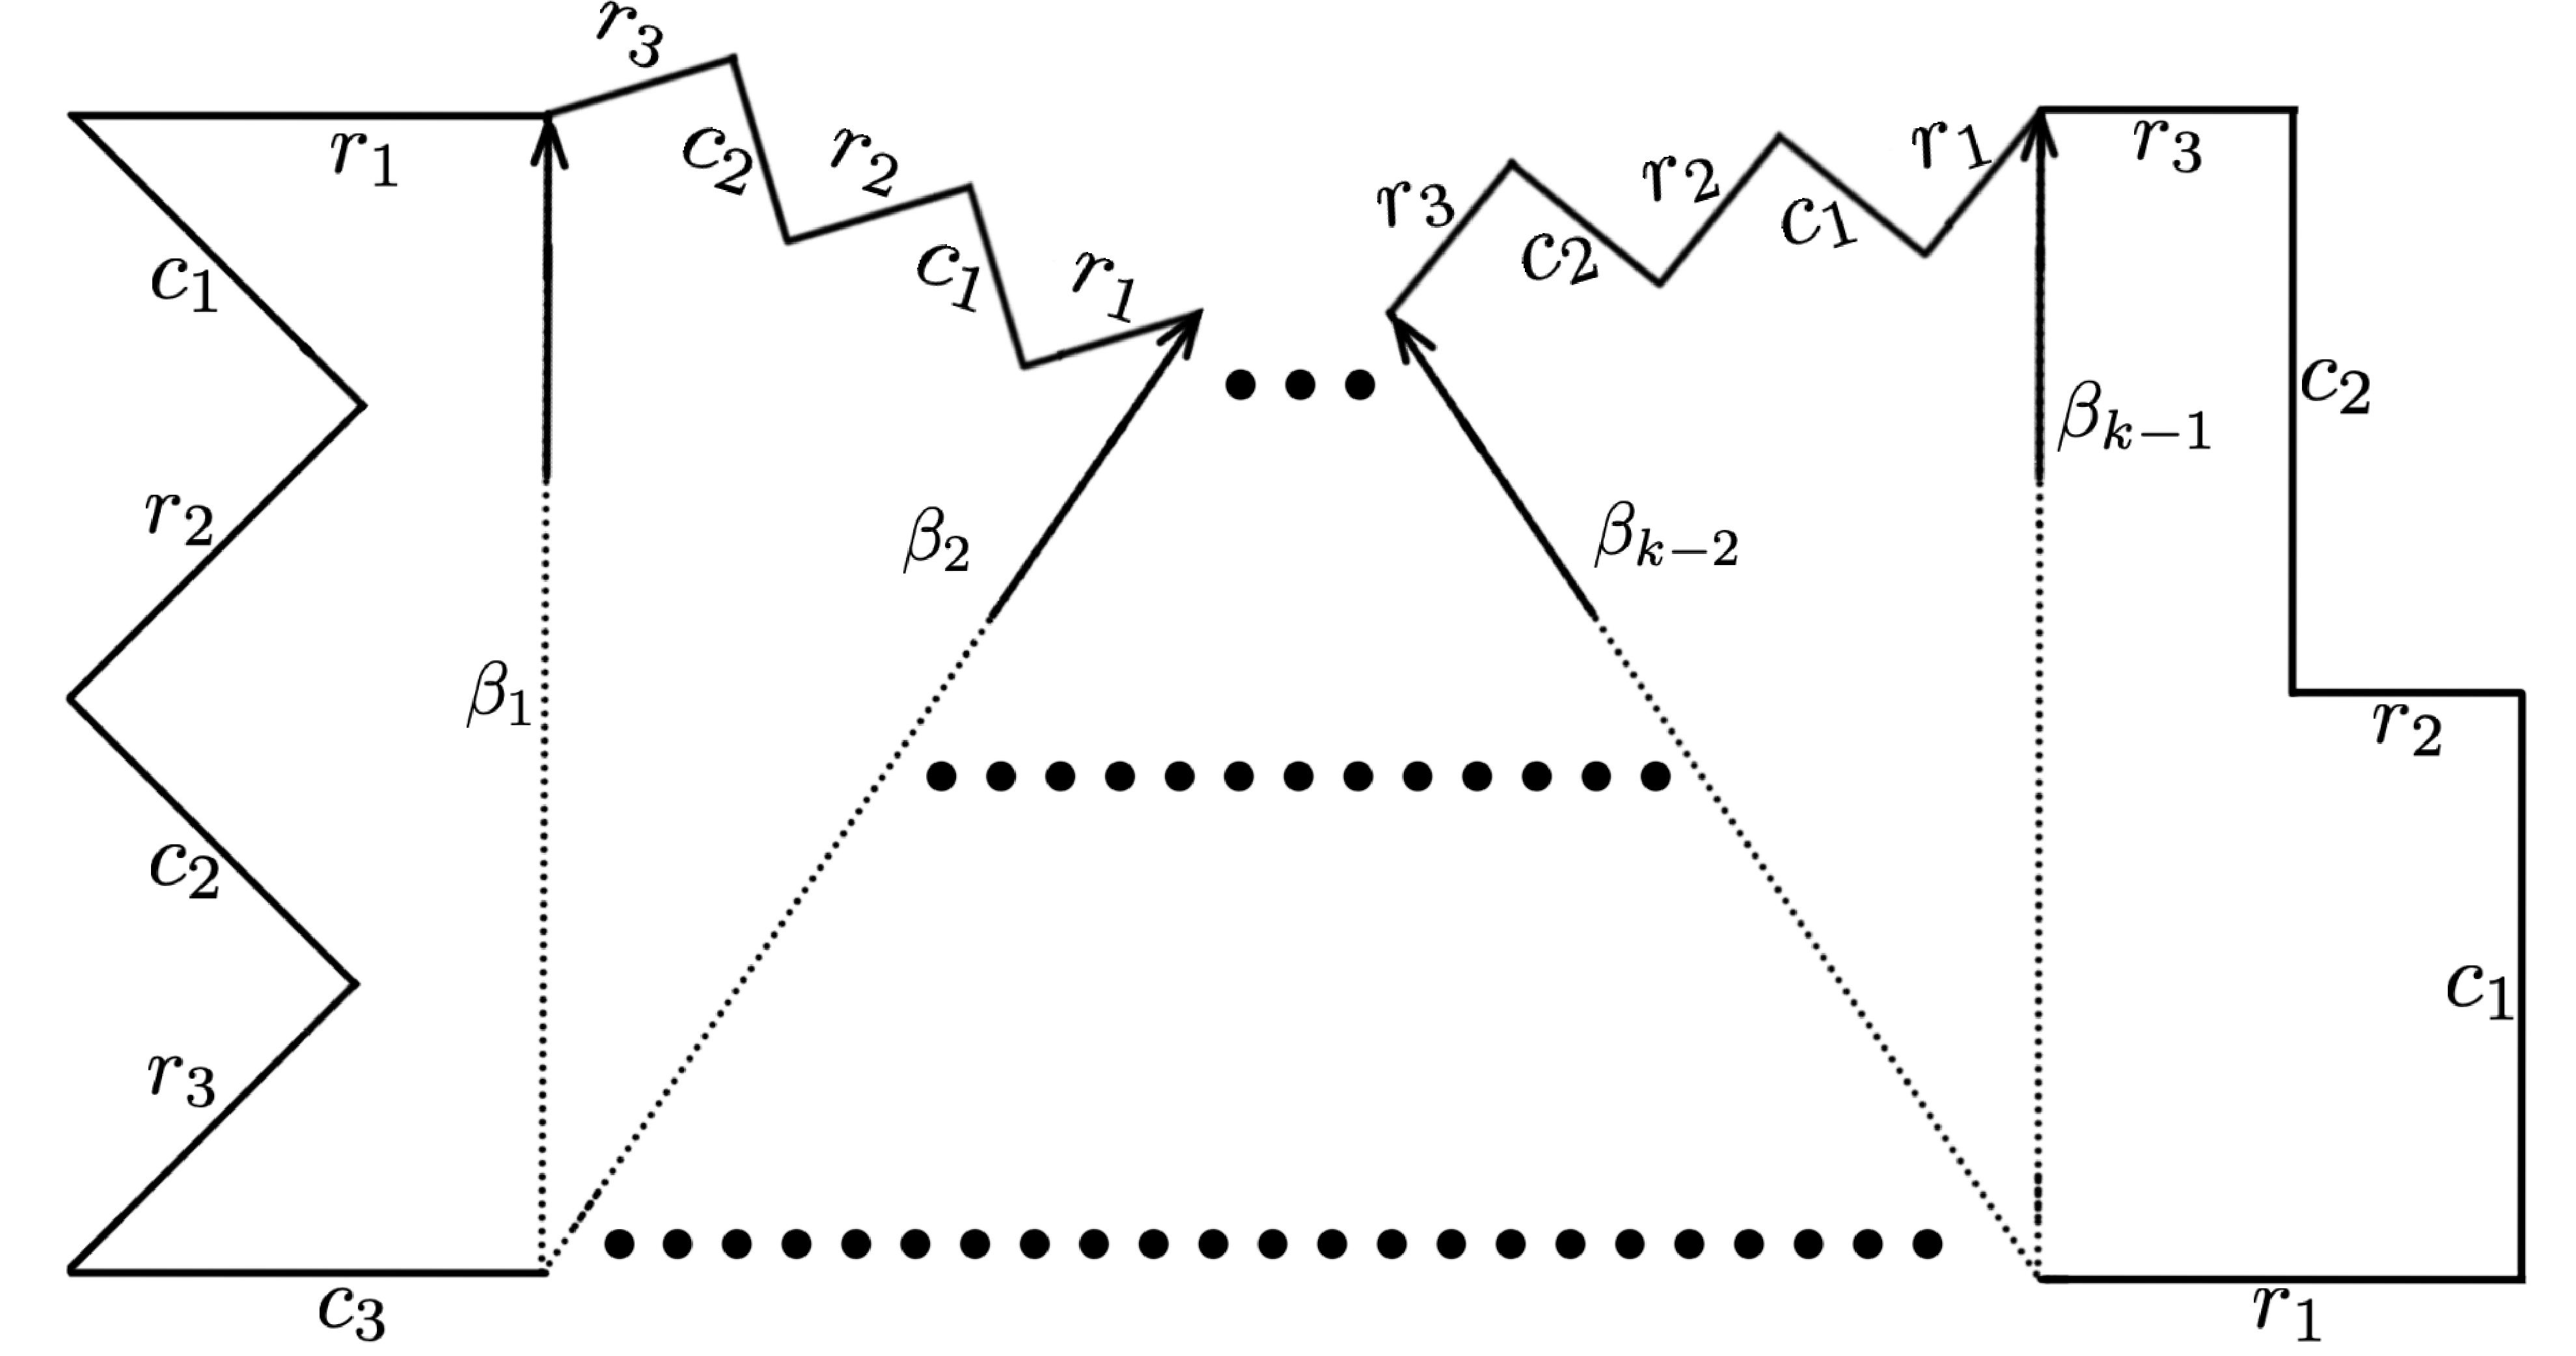
\includegraphics[width=9cm]{images/ch4/section3_circular/atoms/branching/big_domain_transformed.pdf}
%    \caption{Склейка большого листа $\widetilde{\Omega}$.}
    \caption{Область $\widetilde{\Omega}$.}
    \label{fig:pt10:_big_domain_transformed}
\end{figure}

Рассмотрим количество чередований правил склейки $r$ и $c$, возникающих при обходе границы получившегося многоугольника. При этом, если на соседних ребрах склейки указано одно и то же правило склейки, мы объединим эти ребра в одно.
При обходе самого левого листа на рис. \ref{fig:pt10:_big_domain_transformed} правила чередуются трижды. Обход самого правого листа добавит еще два чередования. Каждый из $k-2$ листов посередине добавляет еще по два чередования правил склейки. Таким образом, при обходе границы правила склейки чередуются $3+2+2(k-2) = 2k+1$ раз.

Для получения поверхности $\Xi = \const$ остается склеить четыре многоугольника $\widetilde{\Omega}_1, \ldots, \widetilde{\Omega}_4$ (каждый имеет изображенный на рис. \ref{fig:pt10:_big_domain_transformed} вид) по общим ребрам. 
Склейка листов $\widetilde{\Omega}_1 \cup \widetilde{\Omega}_4$ по правилам склейки $r$ является сферой с $2k+1$ дырками, границы которых проецируются в дуги граничных окружностей или каустик. Аналогично для листов $\widetilde{\Omega}_2 \cup \widetilde{\Omega}_3$. Последующая склейка двух сфер с $2k+1$ с дырками по границам соответствующих дырок будет сферой с $2k$ ручками.

\textit{Случай $C_k'$, где $2 \leq k \leq \left\lfloor \dfrac{r_2^2}{r_2^2-r_1^2} \right\rfloor$} 
устроен аналогично, но вместо  изображенного на рис.    
\ref{fig:pt10:_terminal_max_domain_transformed} в склейке участвует область, изображенная на рис. \ref{fig:pt10:_terminal_max_domain_B1Prime}. Повторяя соображения предыдущего случая получим, что  склейка листов  $\widetilde\Omega_1 \cup \widetilde\Omega_4$ по правилам склейки $r$ является сферой с $2k$ дырками. Склейка с такой же сферой $\widetilde\Omega_2 \cup \widetilde\Omega_3$ по $2k$ дыркам является сферой с $2k-1$ ручками.  

\textit{Случай $C_1$.}

Траектория  <<путешествует>> по единственному листу $\Omega$: сегменты траектории в $\Omega_1$ касаются окружности с радиусом $\rho_1 > r_1$, в области $\Omega_2$ звенья траектории отражаются от дуги $EF$ и  могут перейти в область $\Omega_1$ только через отрезок $FG$ (см. рис. \ref{fig:pt10:_C1_domain}).

Чтобы получить поверхность $S_\Xi$, рассмотрим листы склейки $\widetilde\Omega_1, \ldots, \widetilde\Omega_4$ (каждый имеет вид изображенный как на рис. \ref{fig:pt10:_C1_domain}). Нумерация листов та же, что в \eqref{eq:foc_numeration_circle}. Склейка двух областей $\widetilde{\Omega}_1 \cup \widetilde{\Omega}_4$ по правилу склейки $r$ является сферой с тремя дырками, аналогично для склейки $\widetilde{\Omega}_2 \cup \widetilde{\Omega}_3$. Склейка двух сфер с тремя дырками  по соответствующим границам дырок  является сферой с двумя ручками.

\textit{Случай $C_1'$} рассматривается аналогично. Бильярдная траектория  путешествует по одному листу $\Omega$, изображенному на  рис. \ref{fig:pt10:_C1_domainPrime}. Повтор изложенных выше соображений позволяет заключить, что поверхность в этом случае является тором.
\end{proof}

\subsection{Случай $n_1^2 > n_2^2$}\label{sec:ch5/sec6/sub2}
Напомним, что согласно замечанию \ref{rem:diagram_reuse} диаграмма, изображенная на рис. \ref{fig:pt10:_C_kPrime_definitions} имеет смысл и для  случая $n_1^2 > n_2^2$. Классы $C_m$ и $C_m'$ (см. рис. \ref{fig:pt10:_C_kPrime_definitions}) отличаются друг от друга тем, какое неравенство выполняется листе склейки с наибольшим значением интеграла $\rho_1^2 < r_1^2 < \rho_2^2 < r_2^2$ для класса $C_m$ и $\rho_1^2 < r_1^2 < r_2^2 < \rho_2^2$ для $C_m'$.
\begin{theorem}
В области $\left\{\xi < L_1\right\}$ поверхности $S_\Xi$ являются сферами с $2m+1$ ручками, если $P(\Xi) \in C_m$ и сферами с $2m$ ручками, если $P(\Xi) \in C_m'$ и $m \leq \left\lfloor \frac{r_2^2}{r_2^2-r_1^2} \right\rfloor$. 
\label{th:pt10:th2}
\end{theorem}
\begin{proof}
\textit{Случай $C_k$, где $k\geq2$}. 

Для $n_1^2 > n_2^2$ справедливо утверждение, аналогичное \ref{st:stat_leaf_shapes}:
поверхность $S_\Xi$ получается склейкой нескольких листов, 
а именно:

$\bullet$ одного листа, соответствующего точке $Q$ \textbf{левее} $II_1$ и \textbf{левее} $\widehat{III}$

$\bullet$ одного листа, соответствующего точке $Q$ \textbf{правее} $II_1, \widehat{III}$ и \textbf{левее} $IV_0$.

$\bullet$ и $k-2$ листов, каждый из которых соответствует точкам $Q$   \textbf{правее} $II_1$ и \textbf{левее} $\widehat{III}$.

При этом области будут выглядеть как  изображено на рис. \ref{fig:pt10:_terminal_min_domain_2}--\ref{fig:pt10:_terminal_max_domain_2}

\begin{figure}[!htb]
\minipage{0.33\textwidth}
\centering
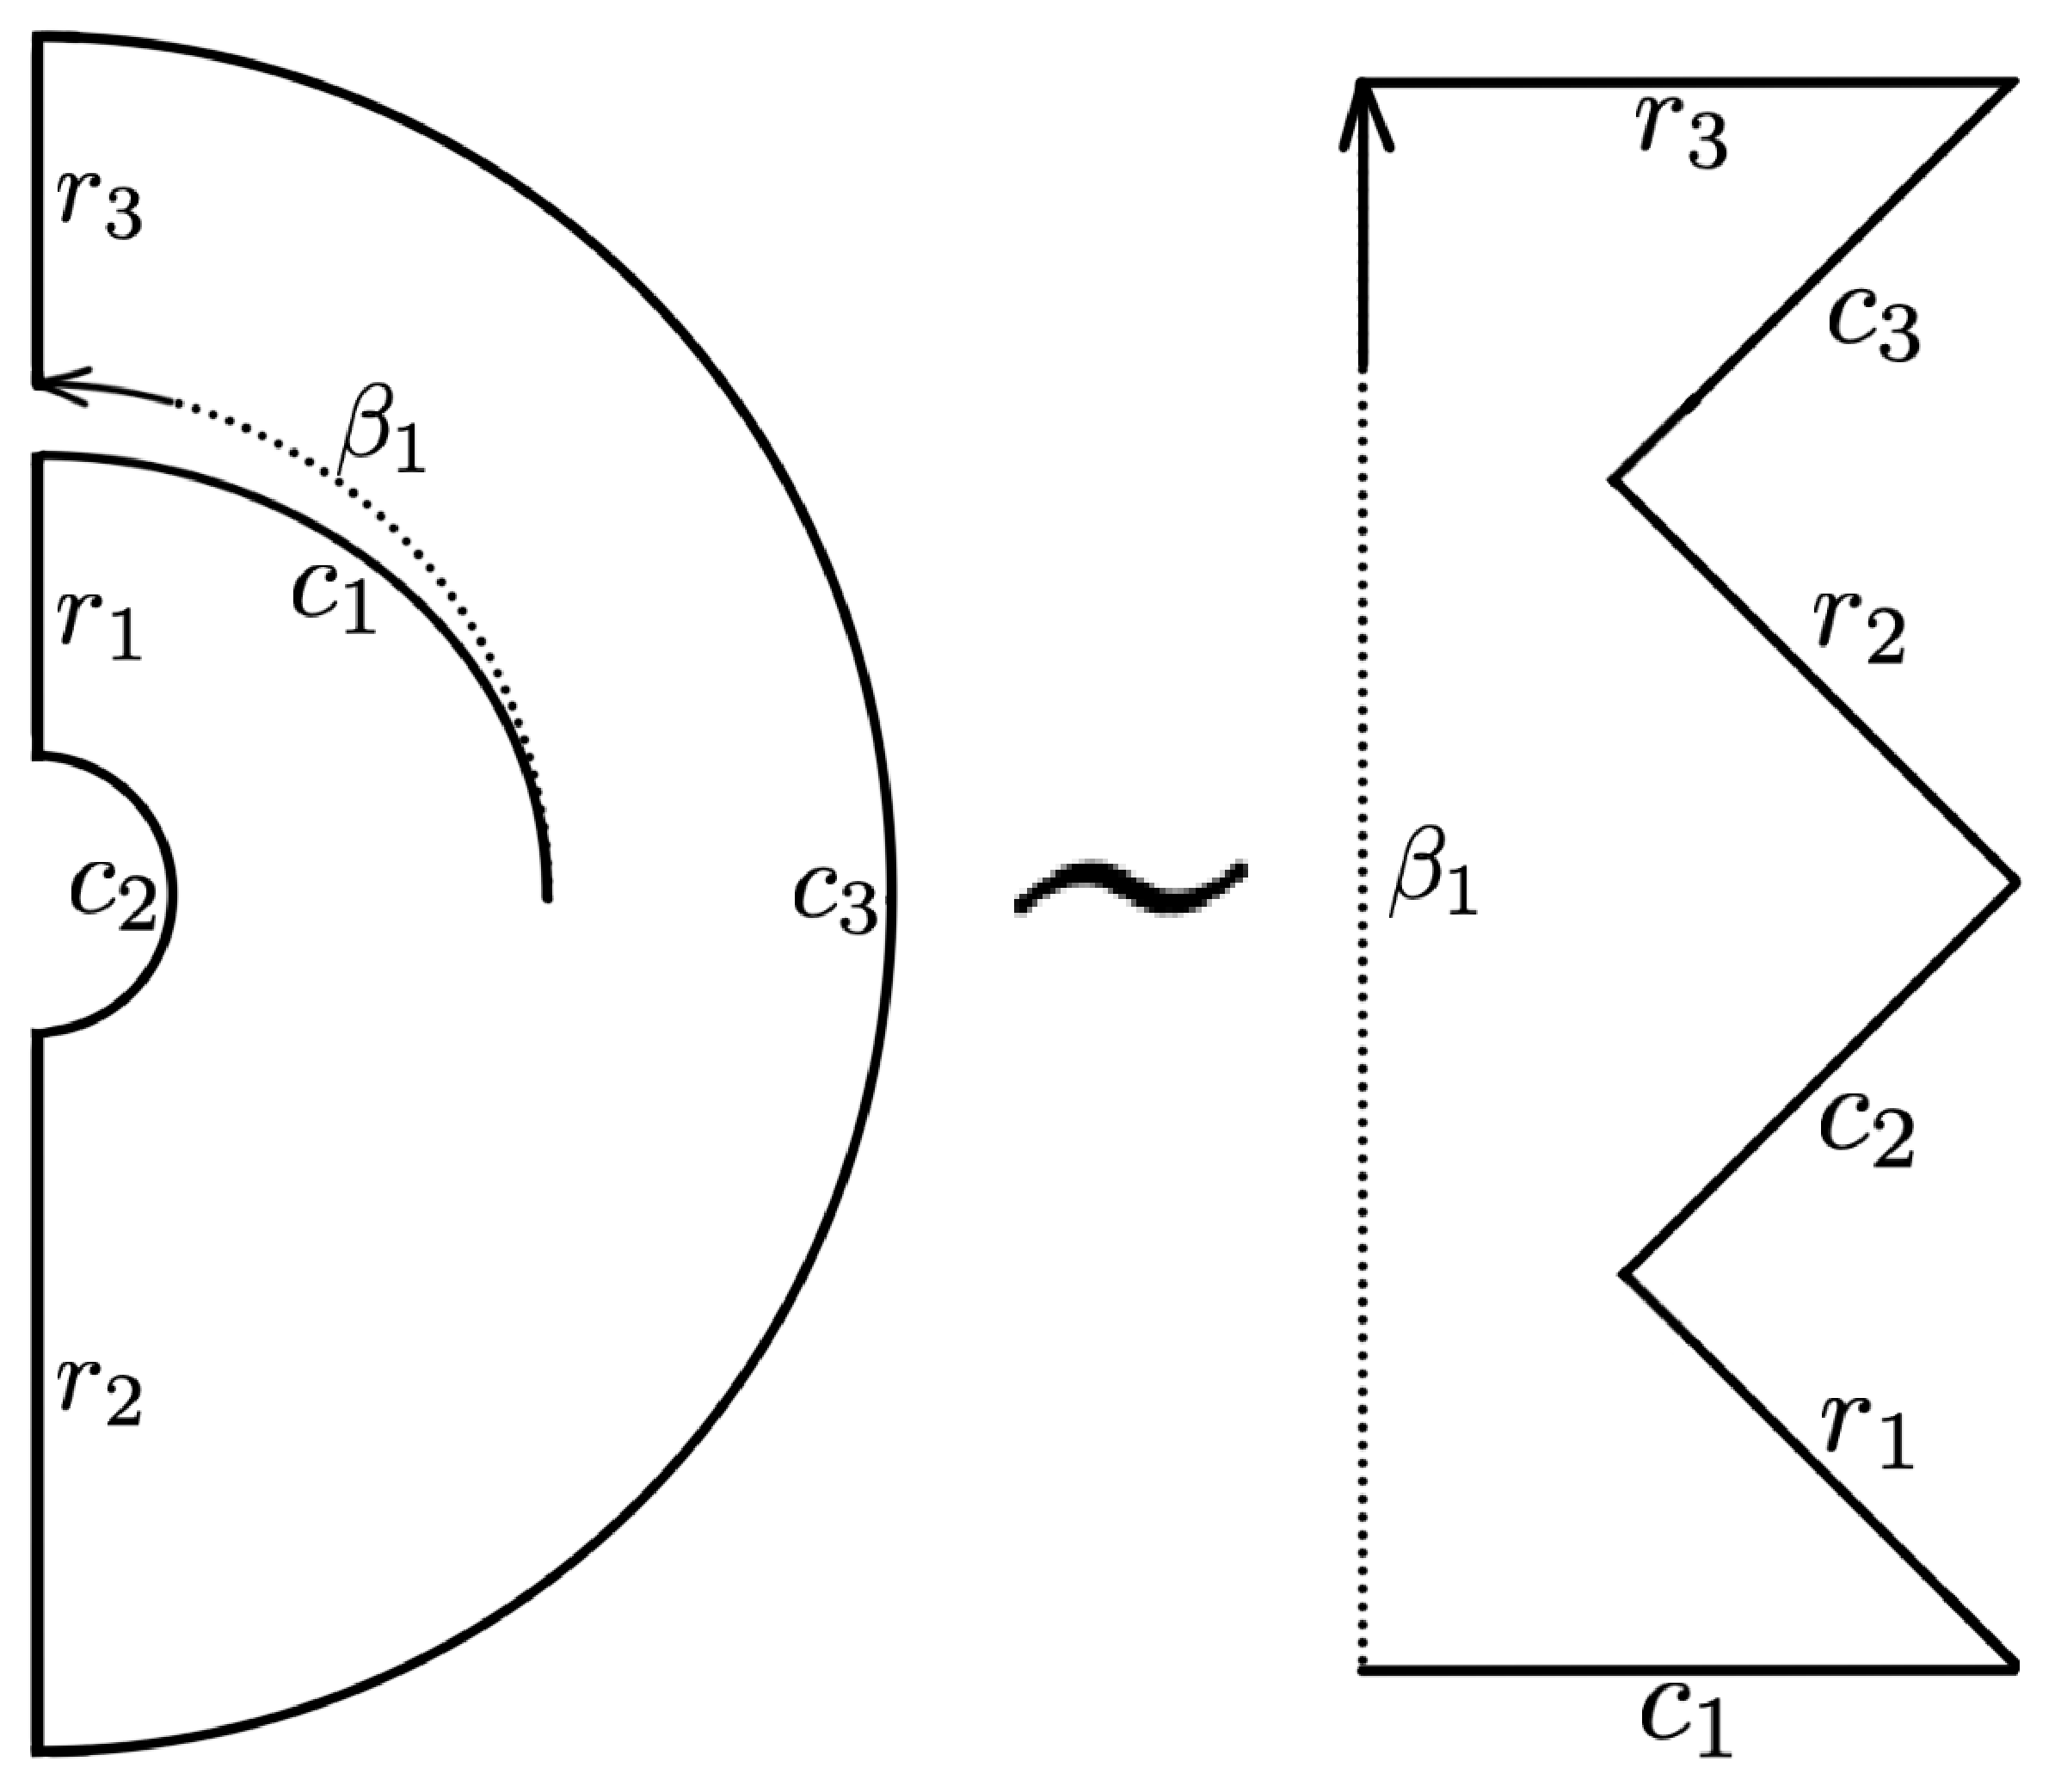
\includegraphics[scale=0.1]{images/ch4/section3_circular/atoms/branching/terminal_min_transformed_2.pdf}
    \caption{Для $Q$ \textbf{левее} $II_1$ и \textbf{левее} $\widehat{III}$.}
    \label{fig:pt10:_terminal_min_domain_2}
\endminipage\hfill
\minipage{0.33\textwidth}
\centering
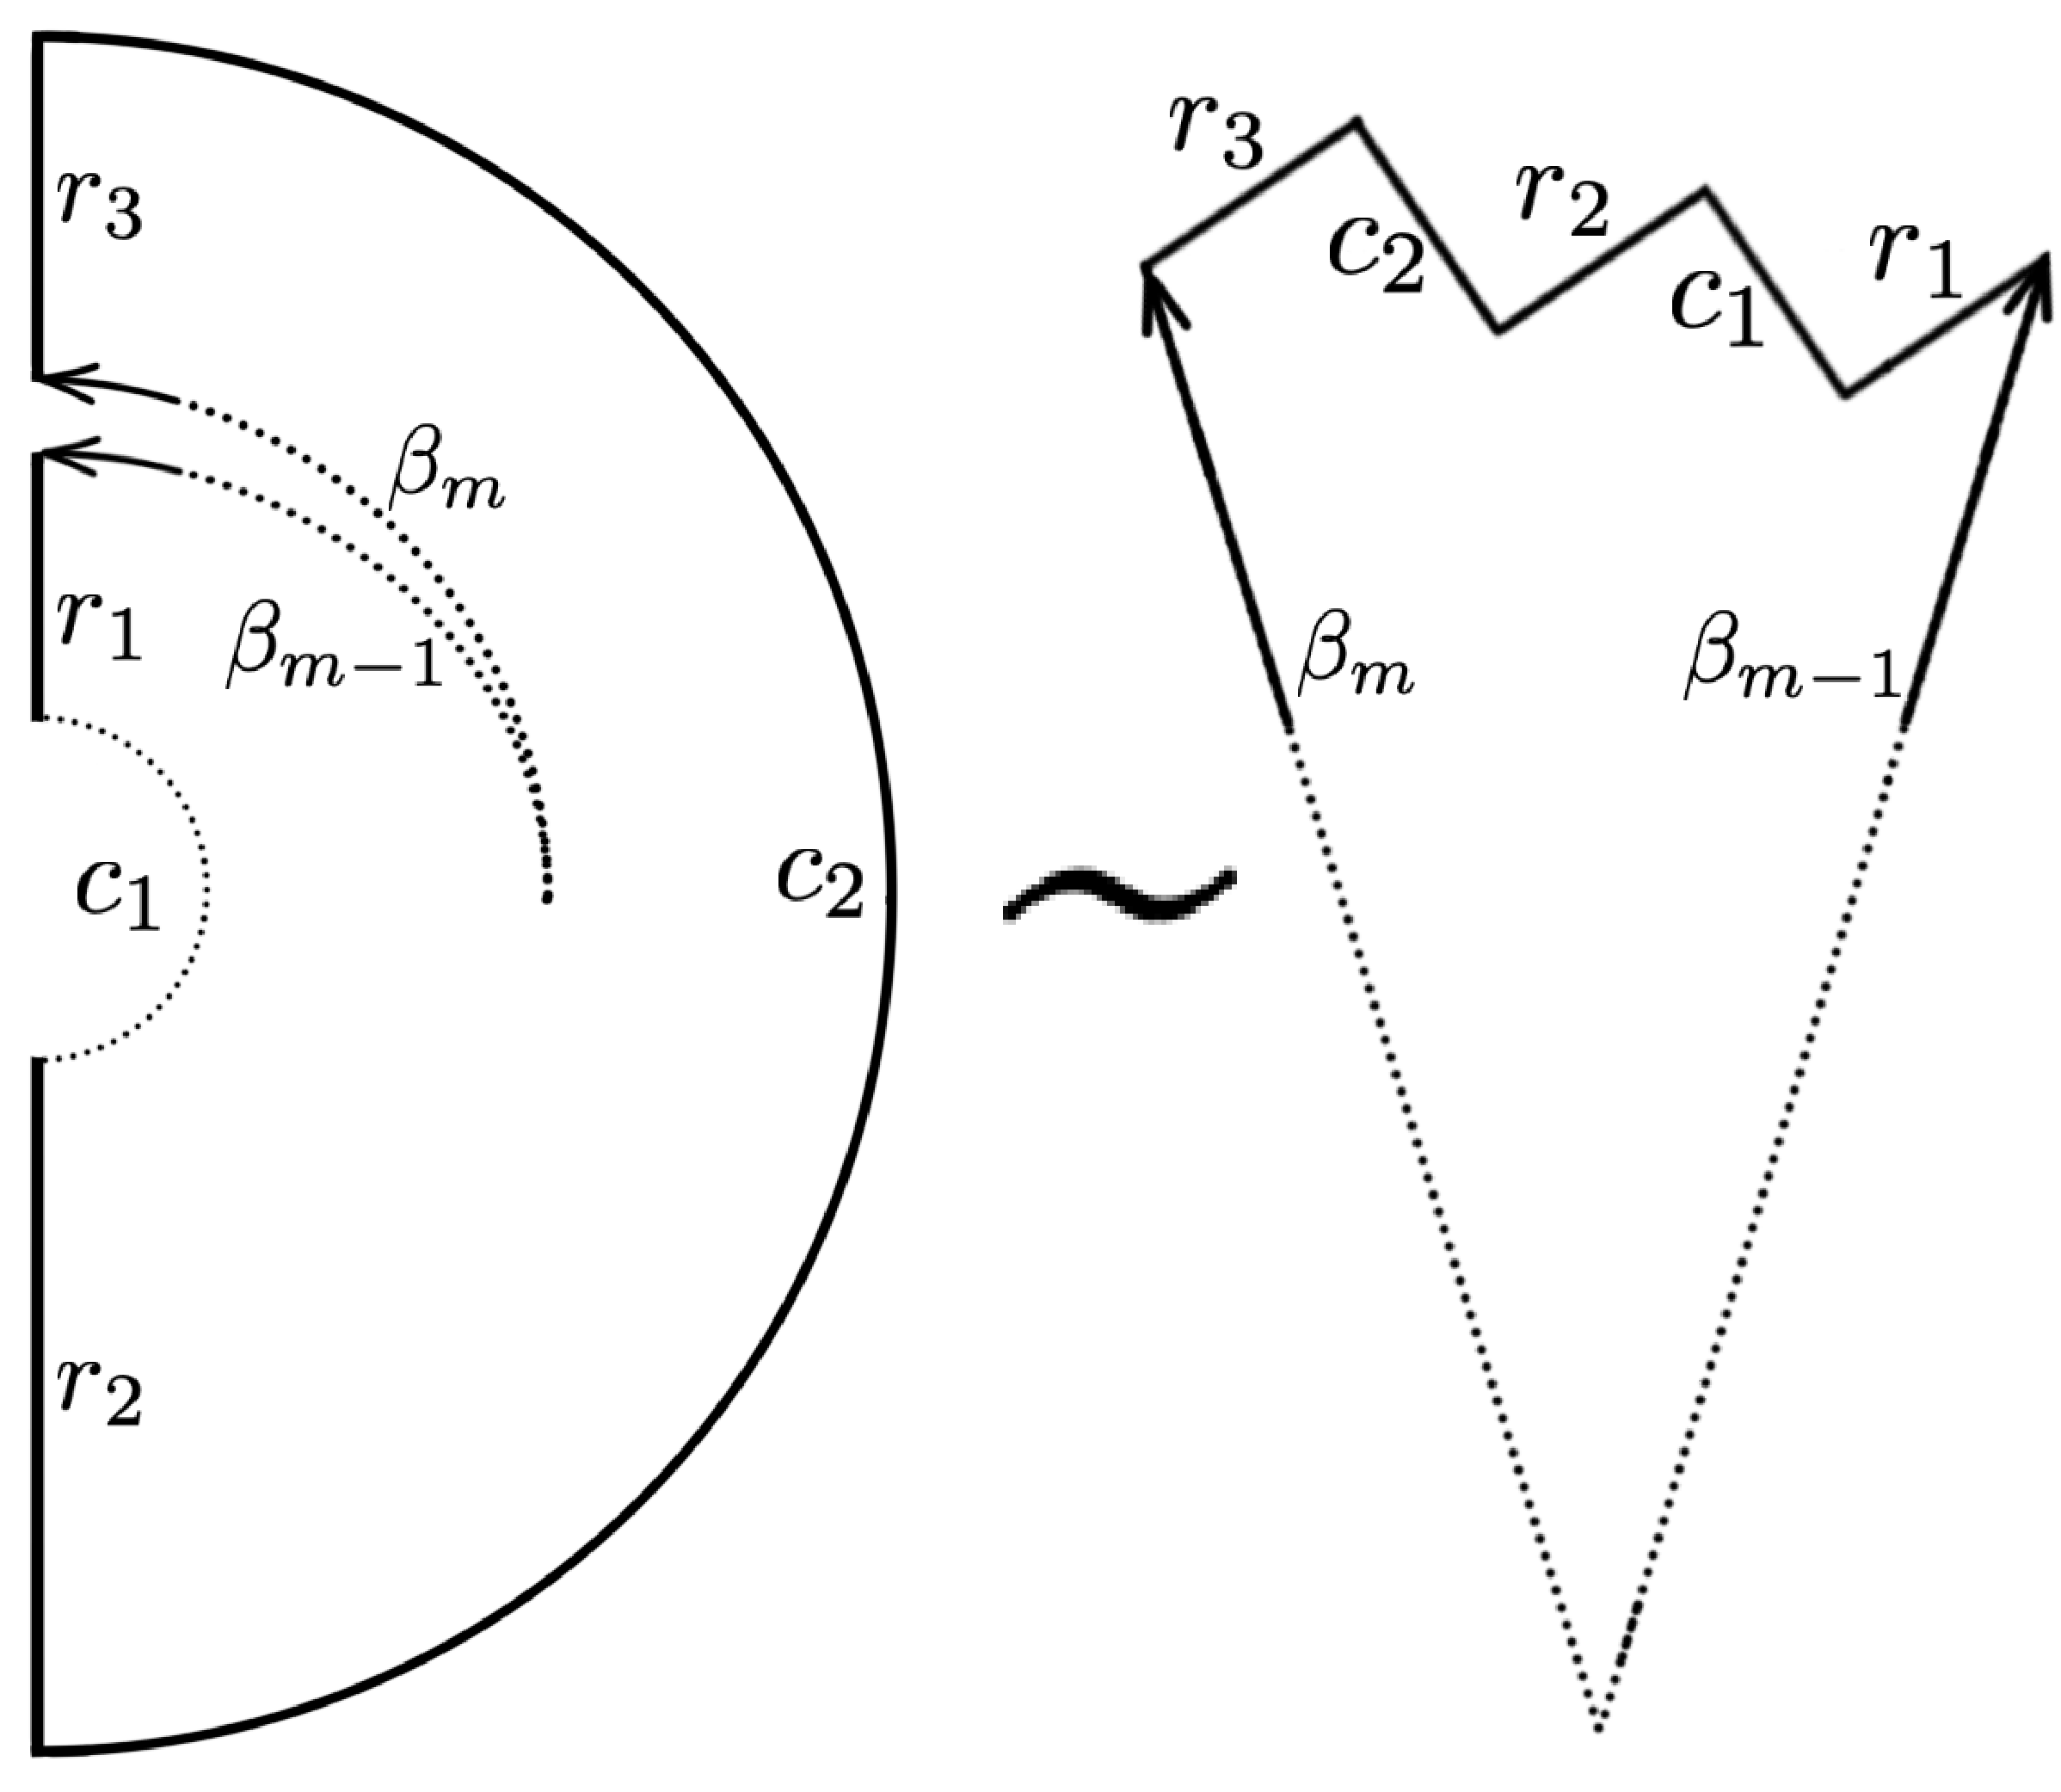
\includegraphics[scale=0.1]{images/ch4/section3_circular/atoms/branching/branching_domain_transformed_2.pdf}
    \caption{Для $Q$ \textbf{правее} $II_1$ и \textbf{левее} $\widehat{III}$.}
    \label{fig:pt10:_branching_domain_2}
\endminipage\hfill
\minipage{0.33\textwidth}
\centering
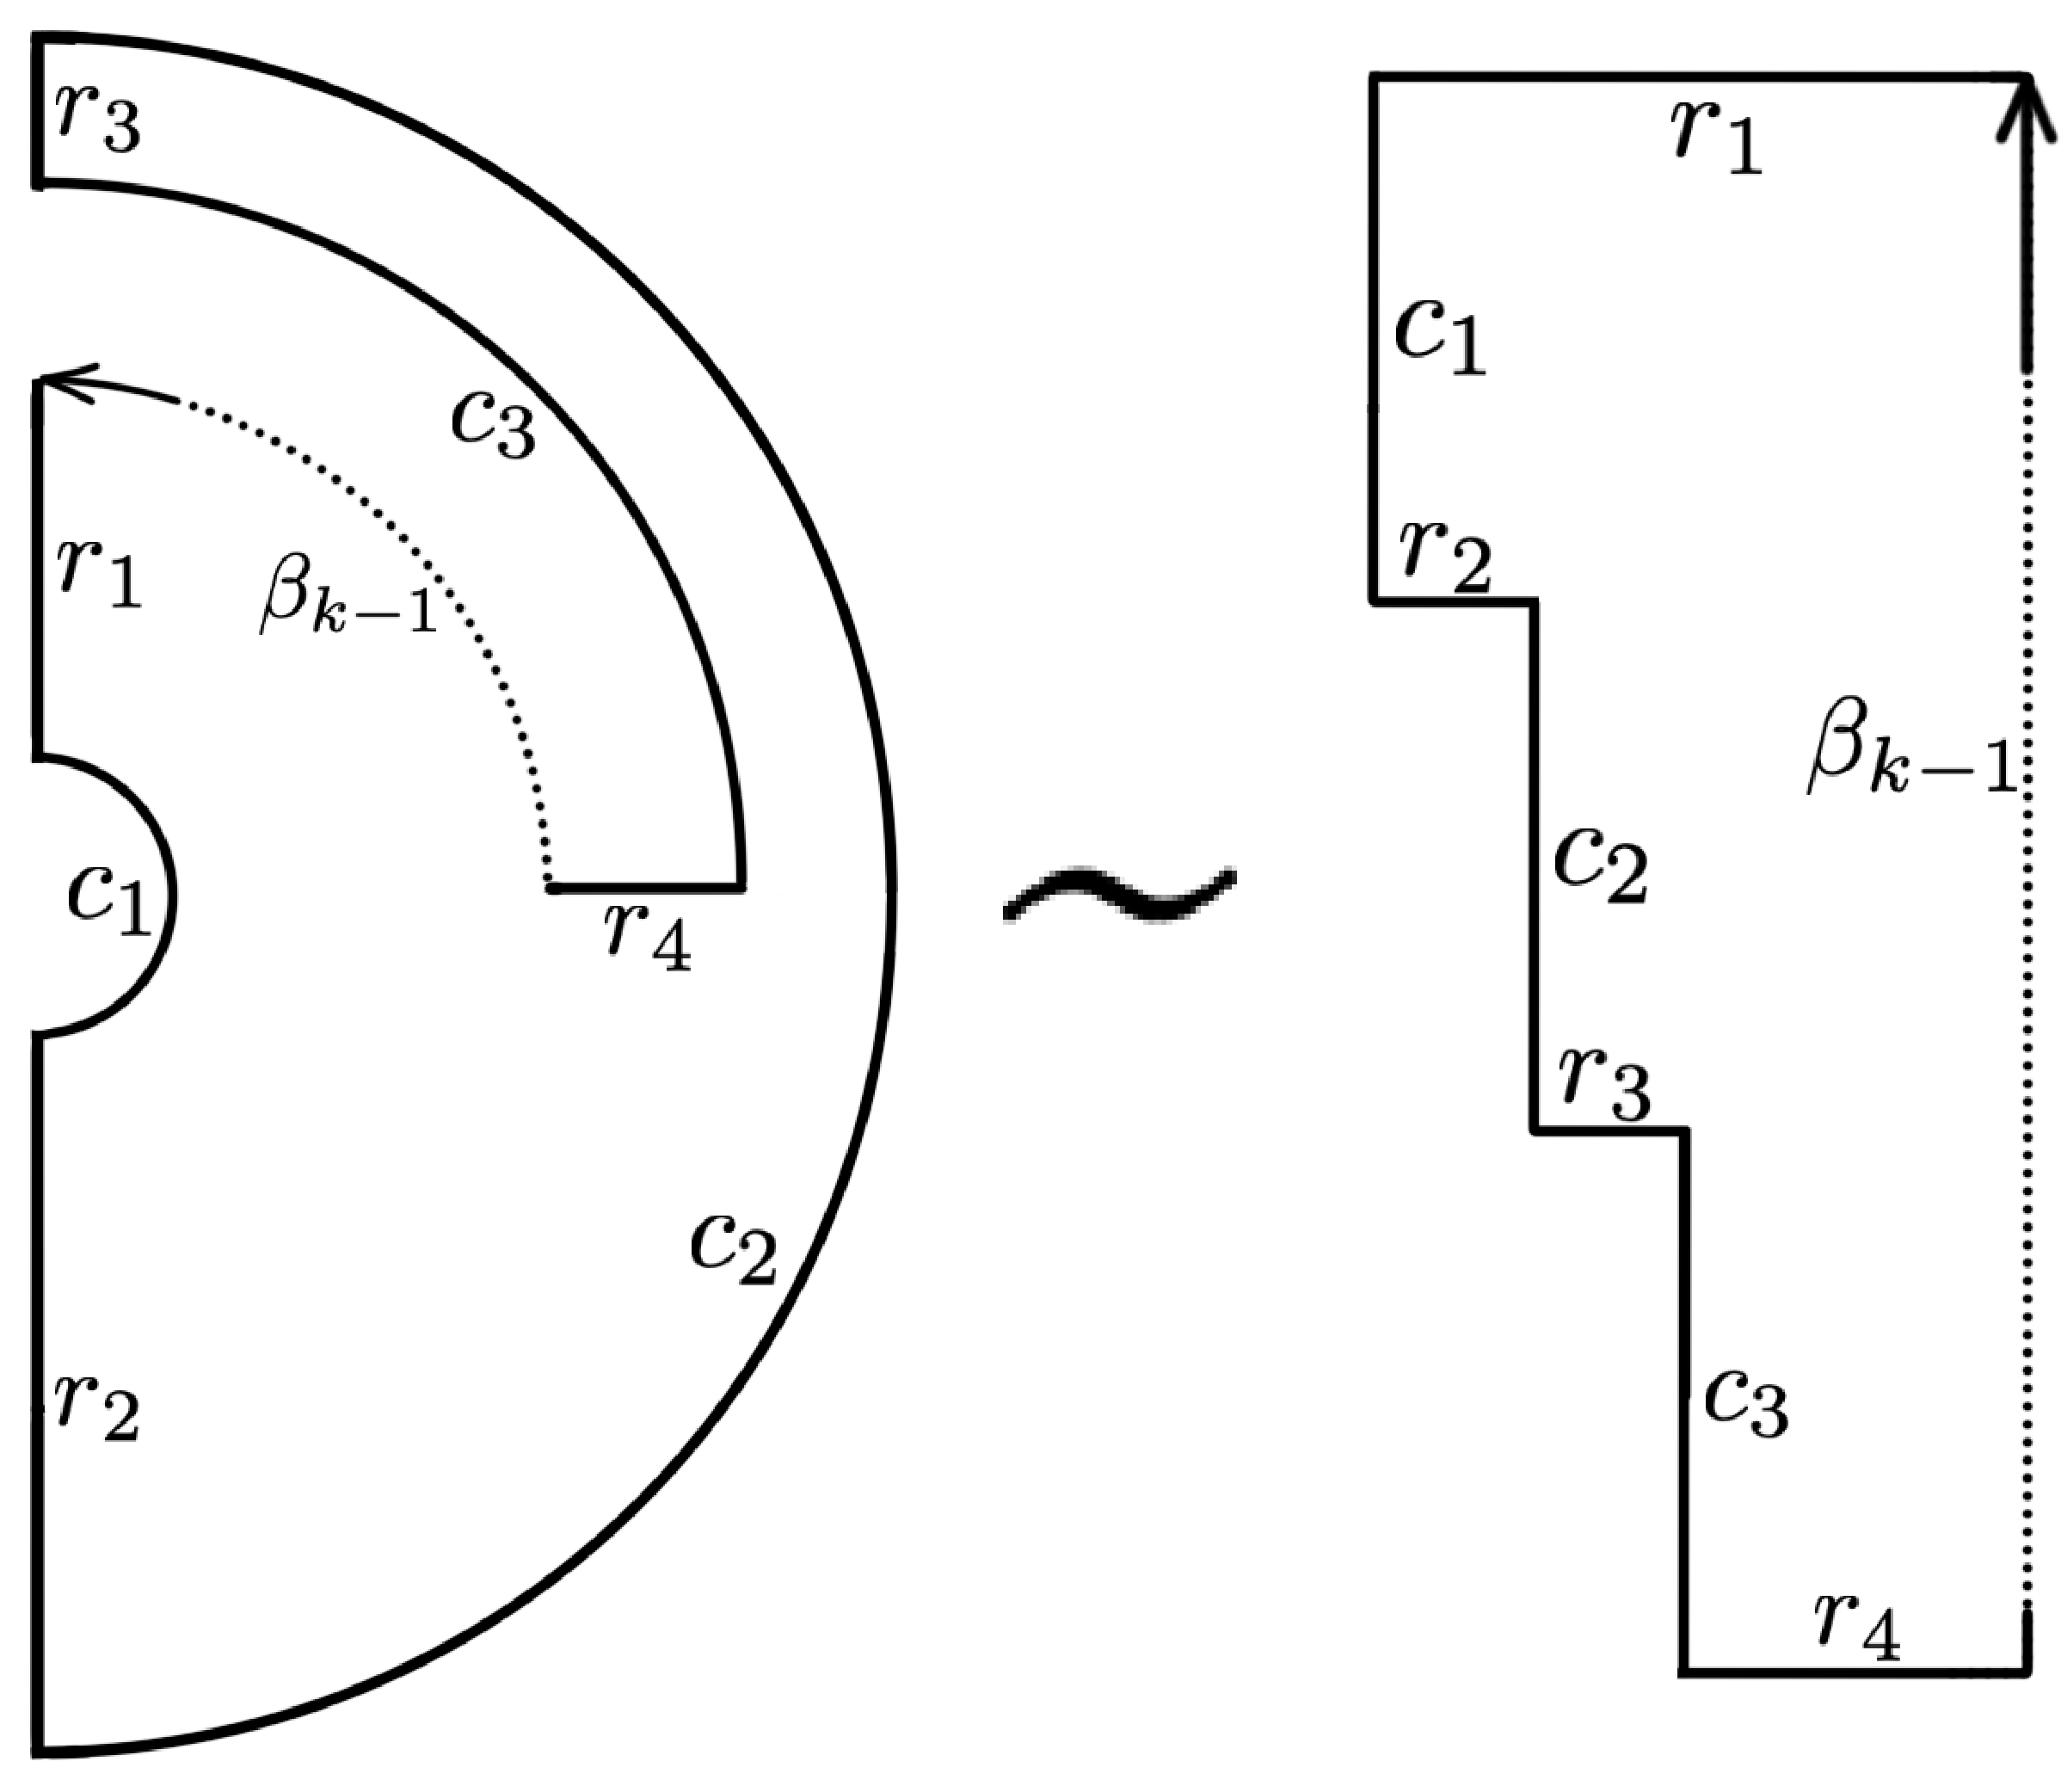
\includegraphics[scale=0.1]{images/ch4/section3_circular/atoms/branching/terminal_max_transformed_2.pdf}
    \caption{Для $Q$ \textbf{правее} $II_1, \widehat{III}$ и \textbf{левее} $IV_0$.}
    \label{fig:pt10:_terminal_max_domain_2}
\endminipage\hfill
\end{figure}

Далее доказательство проводится так же, как в теореме \ref{th:pt10:th1}. Поверхность $S_\Xi$ склеивается из четырех копий области $\widetilde{\Omega}$, показанной на рис. \ref{fig:pt10:_big_domain_transformed_2}. 
Для класса $C_k, k \geq 2$ каждый большой лист получается склейкой изображенных на рис. \ref{fig:pt10:_terminal_min_domain_2}--\ref{fig:pt10:_terminal_max_domain_2} листов вдоль одноименных склеек $\beta_1, \ldots, \beta_{k-1}$ (см. рис. \ref{fig:pt10:_big_domain_transformed_2}).

\begin{figure}[!htb]
\centering
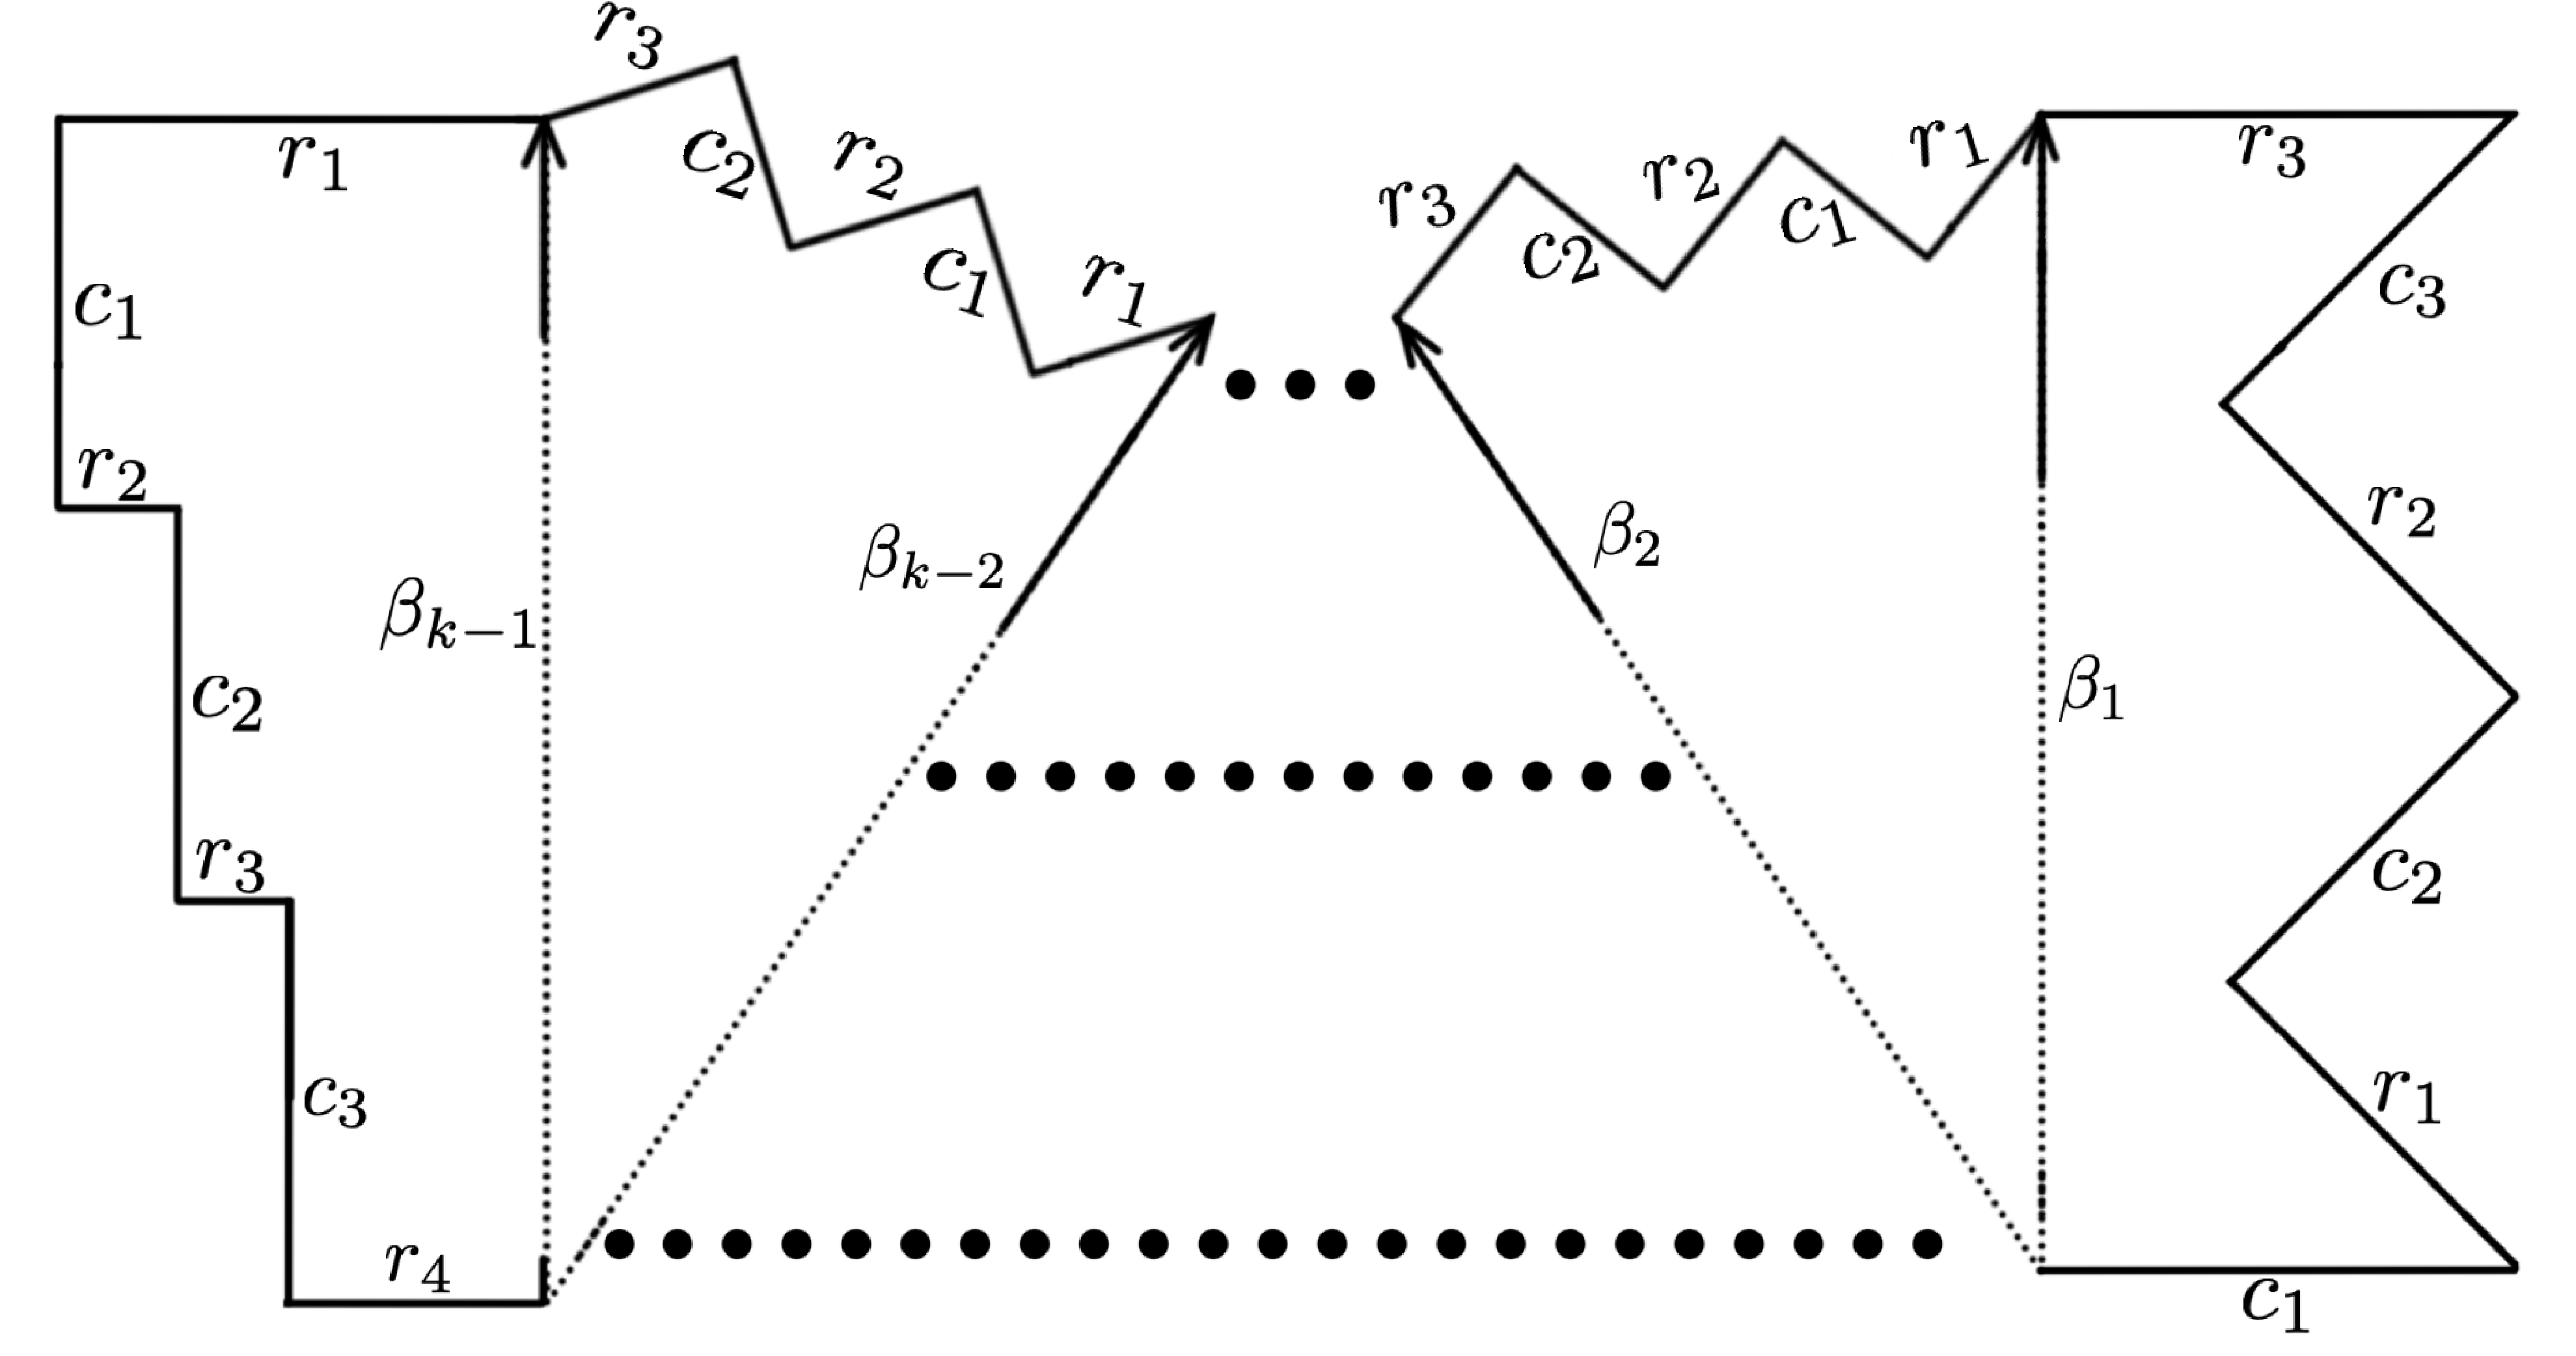
\includegraphics[width=9cm]{images/ch4/section3_circular/atoms/branching/big_domain_transformed_2.pdf}
%    \caption{Склейка большого листа $\widetilde{\Omega}$.}
    \caption{}

    \label{fig:pt10:_big_domain_transformed_2}
\end{figure}

Правила склейки $r$ и $c$ на границе левого листа чередуются трижды, так же как на границе правого листа. Каждый из $k-2$ листов между ними вносит по два чередования. Тогда на границе $\widetilde{\Omega}$ правила склейки чередуются $3+3+2(k-2) = 2k+2$ раз. 
Так же как в доказательстве теоремы \ref{th:pt10:th1} заключаем, что  поверхность $S_\Xi$ является сферой с $2k+1$ ручками.

\textit{Случай $C_k', k\geq 2$}, рассматривается аналогично, но вместо листа, изображенного на рис. \ref{fig:pt10:_terminal_max_domain_2} участвует лист, показанный на рис. \ref{fig:pt10:_Ck_prime_domain}. Как видно, отличия от рис. \ref{fig:pt10:_terminal_max_domain_2} заключаются в отсутствии $r_3$ и $c_3$, а также в том, что дуга $r_4$ продолжается до пересечения с  $c_2$. Повторяя соображения выше, получим, что склейка $\widetilde{\Omega}_1 \cup \widetilde{\Omega}_4$ по правилу склейки $r$ является сферой с $2k + 1$ дырками. Вся поверхность является сферой с $2k$ ручками.

\textit{Случай $C_1$.} Траектория <<путешествует>> по одному листу $\Omega$: сегменты траектории в области $\Omega_2$ касаются окружности с радиусом $\rho_2 > r_1$, в области $\Omega_1$ звенья траектории отражаются от дуги $EF$ (см. рис. \ref{fig:pt10:_C1_domain_2}).

\begin{figure}[!htb]
\minipage{0.33\textwidth}
\centering
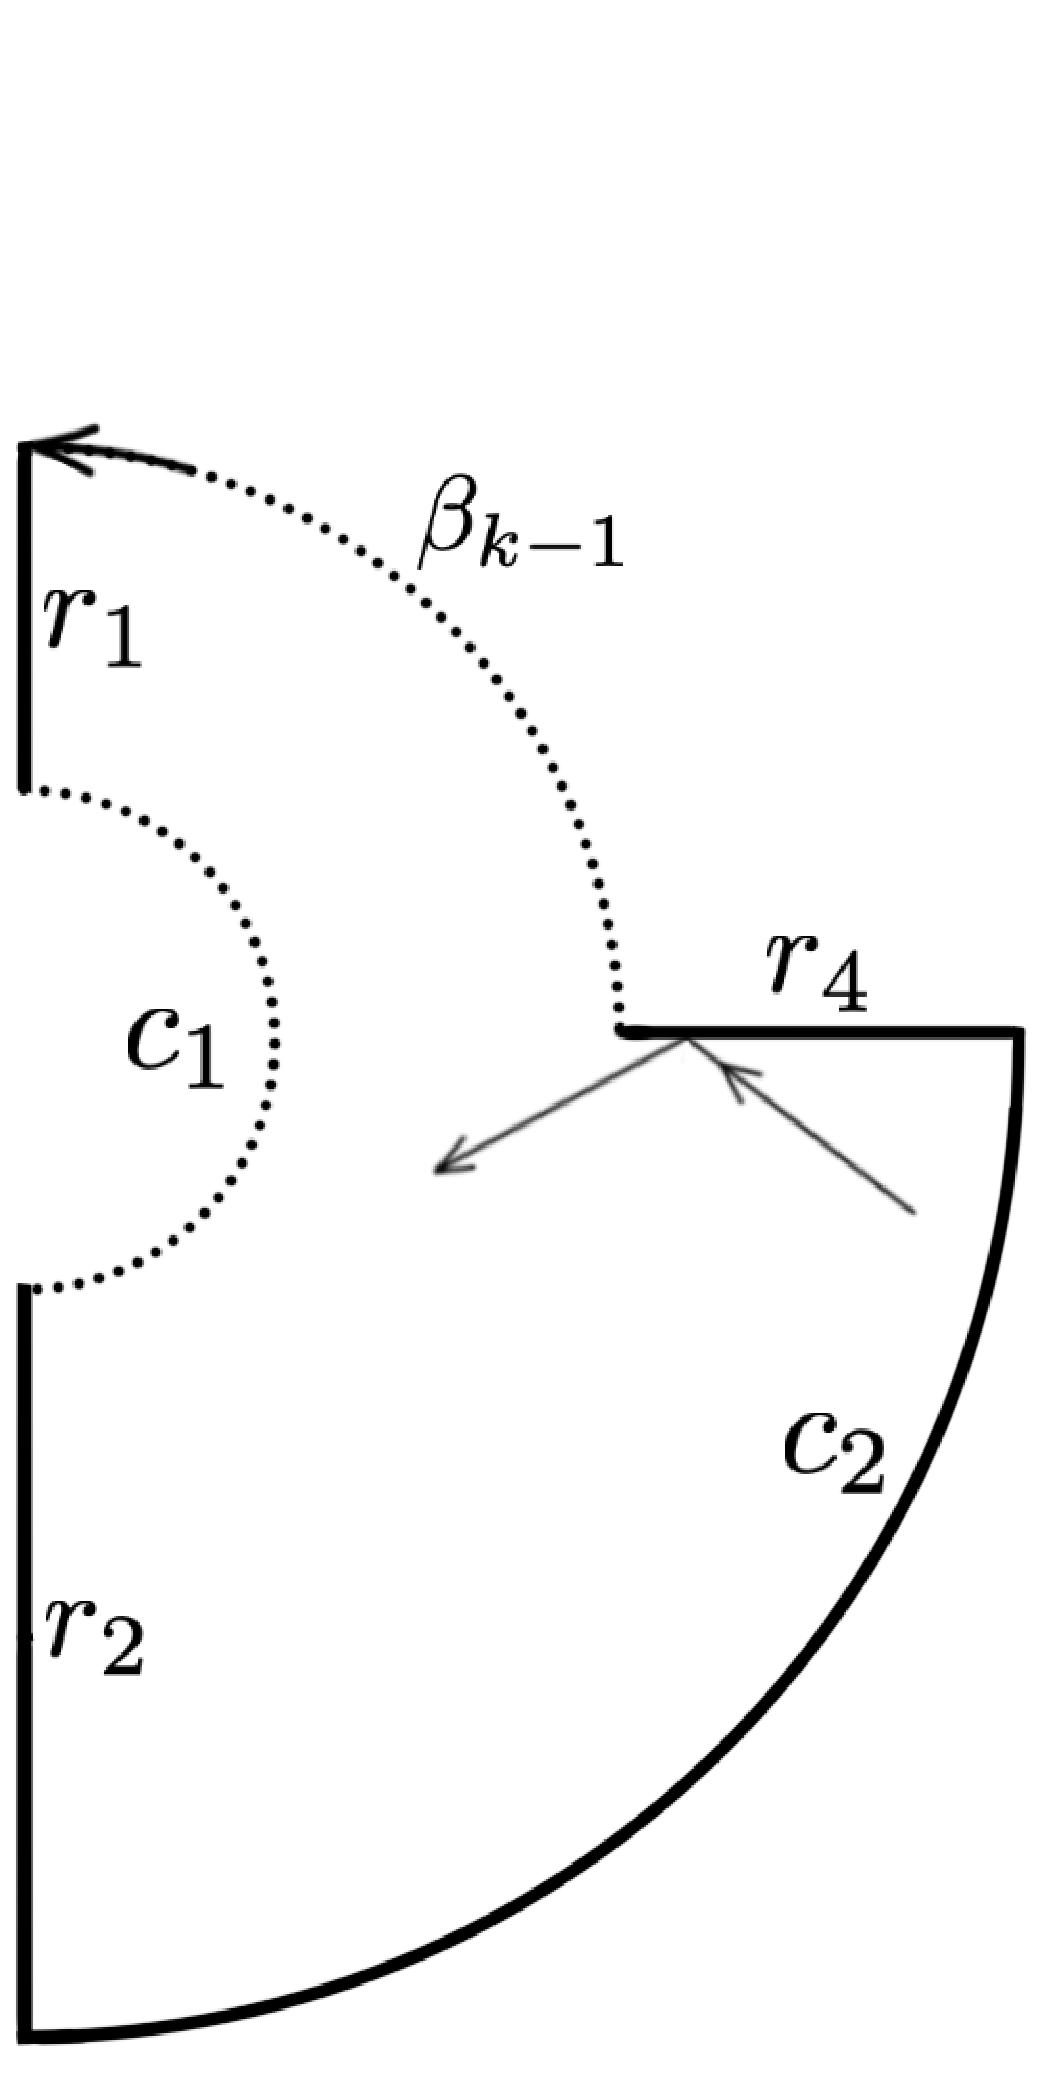
\includegraphics[width=2cm]{images/ch4/section3_circular/atoms/branching/sect3_Ck_prime_domain.pdf}
    \caption{Склейка листа $\widetilde{\Omega}$ для случая $C_k'$.}
    \label{fig:pt10:_Ck_prime_domain}
    \endminipage\hfill
\minipage{0.33\textwidth}
\centering
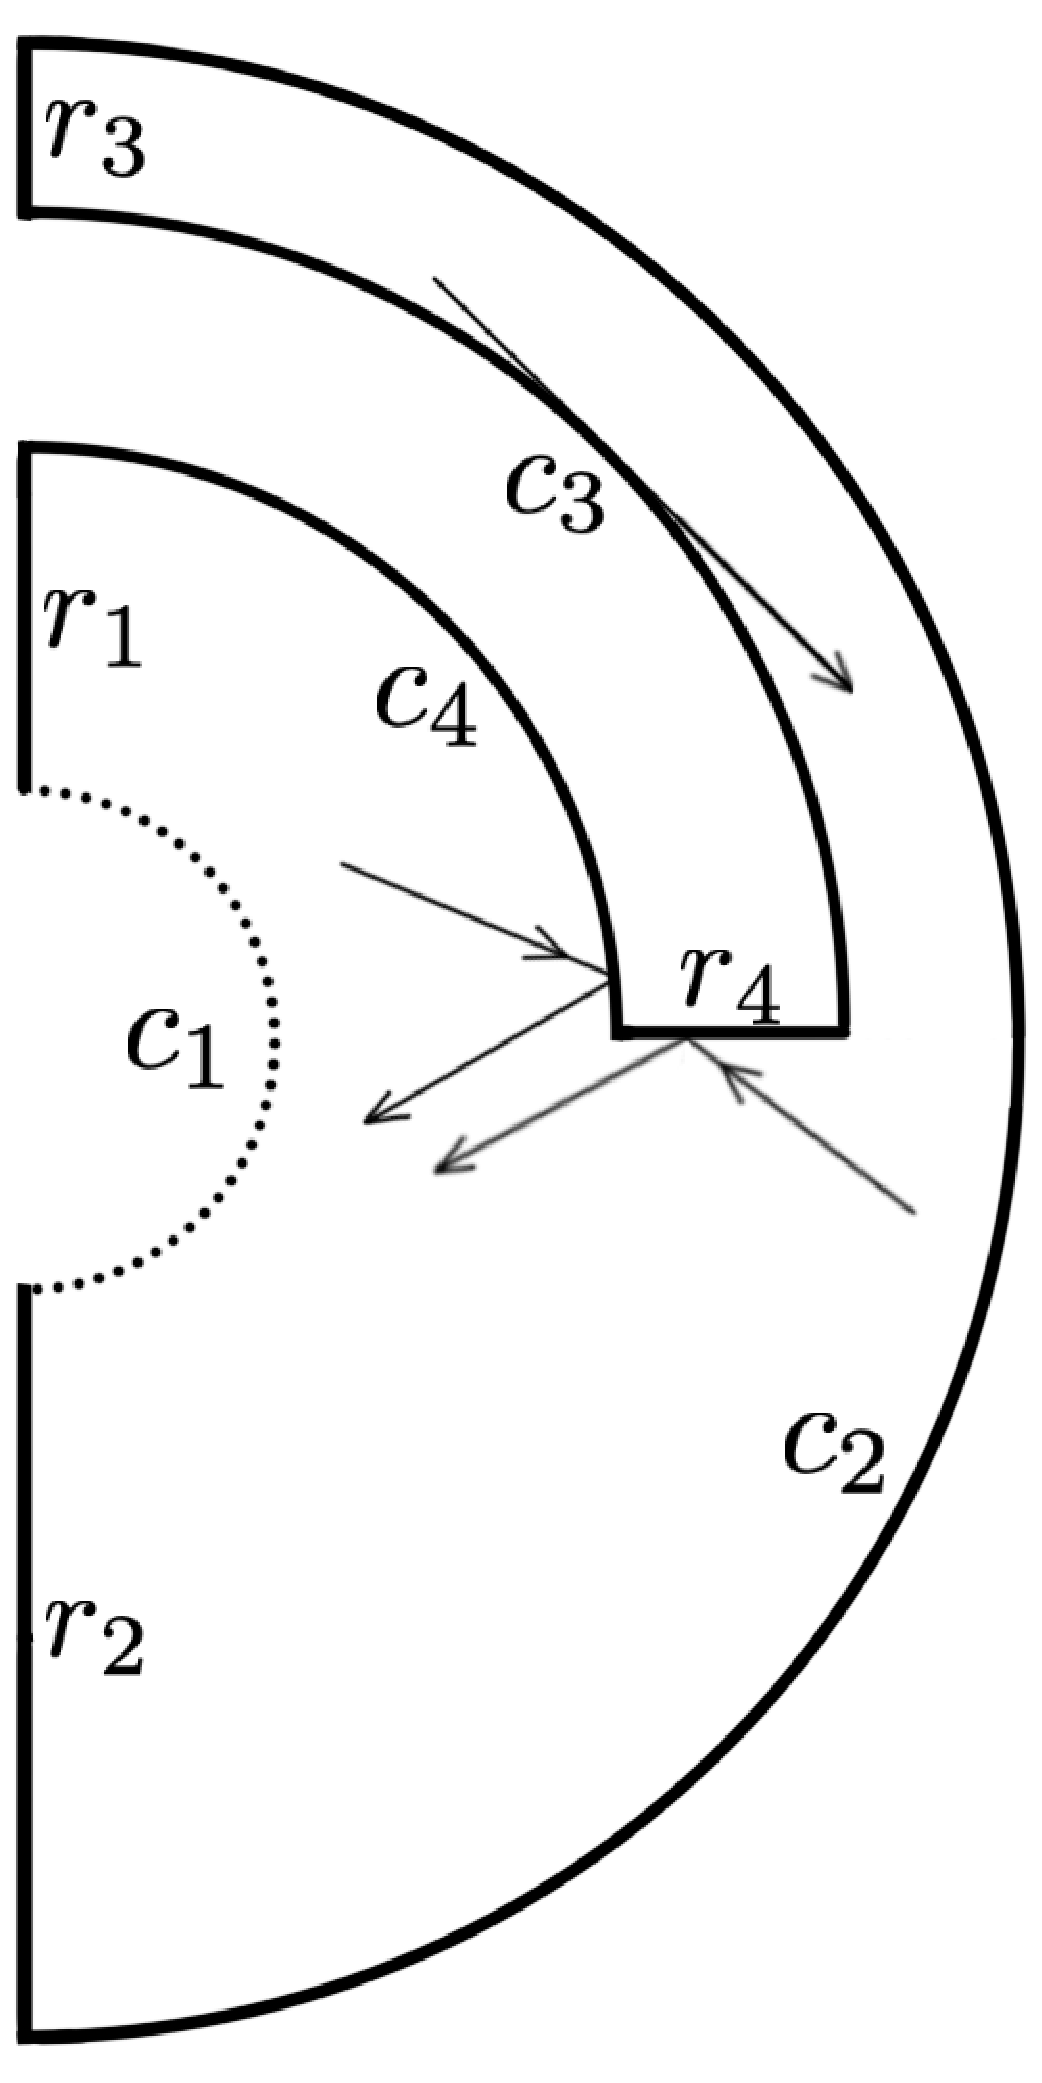
\includegraphics[width=2cm]{images/ch4/section3_circular/atoms/branching/sect3_C1_domain_2.pdf}
    \caption{Склейка листа $\widetilde{\Omega}$ для случая $C_1$. Определения $r$ и $c$ см. \eqref{eq:RCrules_circle}.}
    \label{fig:pt10:_C1_domain_2}
    \endminipage\hfill
\minipage{0.33\textwidth}
\centering
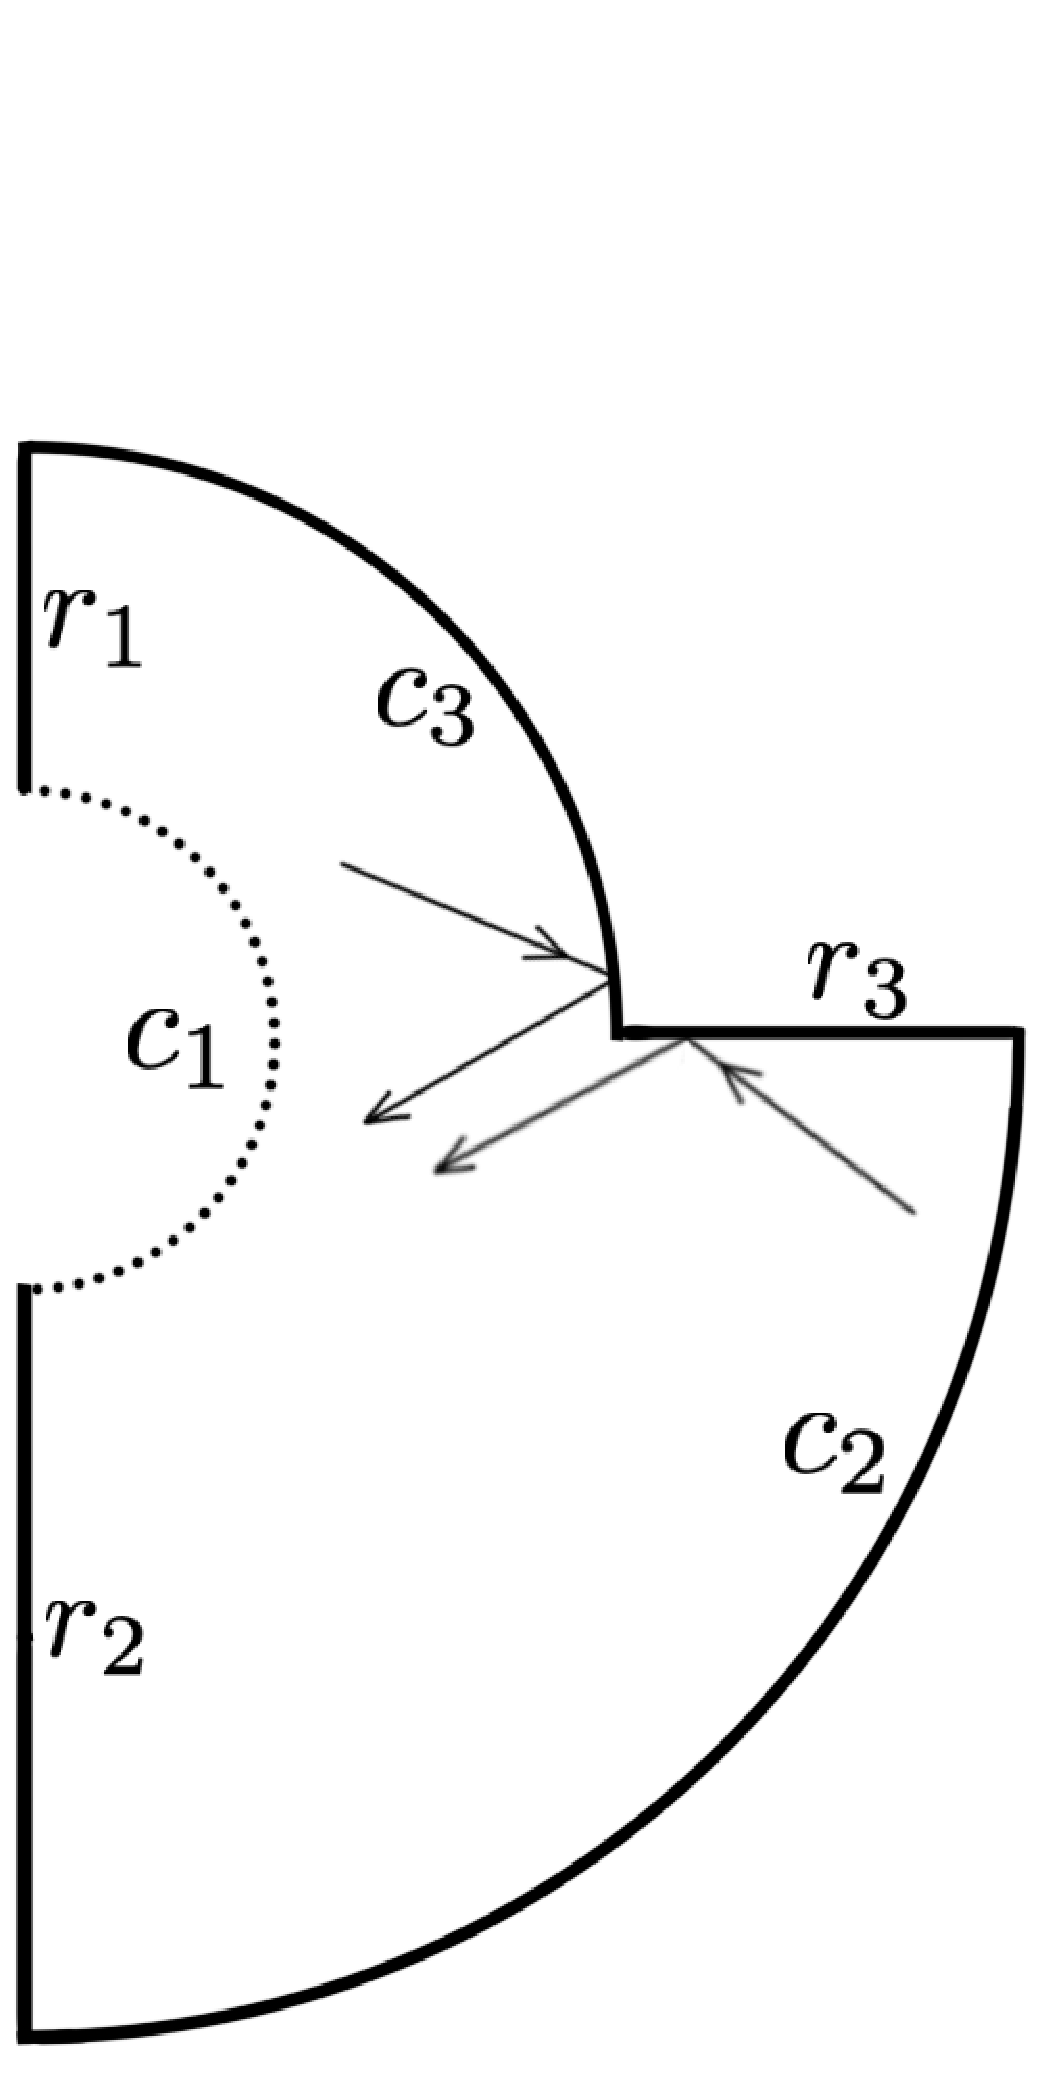
\includegraphics[width=2cm]{images/ch4/section3_circular/atoms/branching/sect3_C1Prime_domain_2.pdf}
    \caption{Склейка листа $\widetilde{\Omega}$ для случая $C_1'$. Определения $r$ и $c$ см. \eqref{eq:RCrules_circle}.}
    \label{fig:pt10:_C1_prime_domain_2}
\endminipage\hfill
\end{figure}


Определим векторы скорости как в \eqref{eq:foc_numeration_circle}. Склейка двух областей $\widetilde{\Omega}_1 \cup \widetilde{\Omega}_4$ по правилу склейки $r$ является сферой с четырьмя дырками, аналогично для склейки $\widetilde{\Omega}_2 \cup \widetilde{\Omega}_3$. Склейка двух сфер с четырьмя дырками является сферой с тремя ручками.

\textit{Случай $C_1'$.} Траектория <<путешествует>> по одному листу $\Omega$, изображенному на рис. \ref{fig:pt10:_C1_prime_domain_2}. Тогда $\widetilde{\Omega}_1 \cup \widetilde{\Omega}_4$ является сферой с тремя дырками. Следовательно, вся поверхность является сферой с двумя ручками.
\end{proof}

\section{Неособые поверхности для случая $\left\{\xi > L_1\right\}$}\label{sec:ch5/sec7}
Этот случай существенно проще предыдущего, поскольку в этом случае дополнительный интеграл $\Xi$ однозначен. Поэтому бильярдные траектории лежат на поверхностях уровня дополнительного интеграла $\Xi=\const$.
%В области $\left\{\xi > L_1\right\}$ поверхности соответствуют уровням интеграла 

%На рис. \ref{fig:pt10:_xiL1_subdivision} показано, на какие области разбивается область $\left\{\xi > L_1 \right\}$
Область $\left\{\xi > L_1 \right\}$ (см. рис. \ref{fig:pt10:_lineDomains_simple}) разбивается  на четыре области, показанные на рис. \ref{fig:pt10:_xiL1_subdivision}.
\begin{figure}[!htb]
\centering
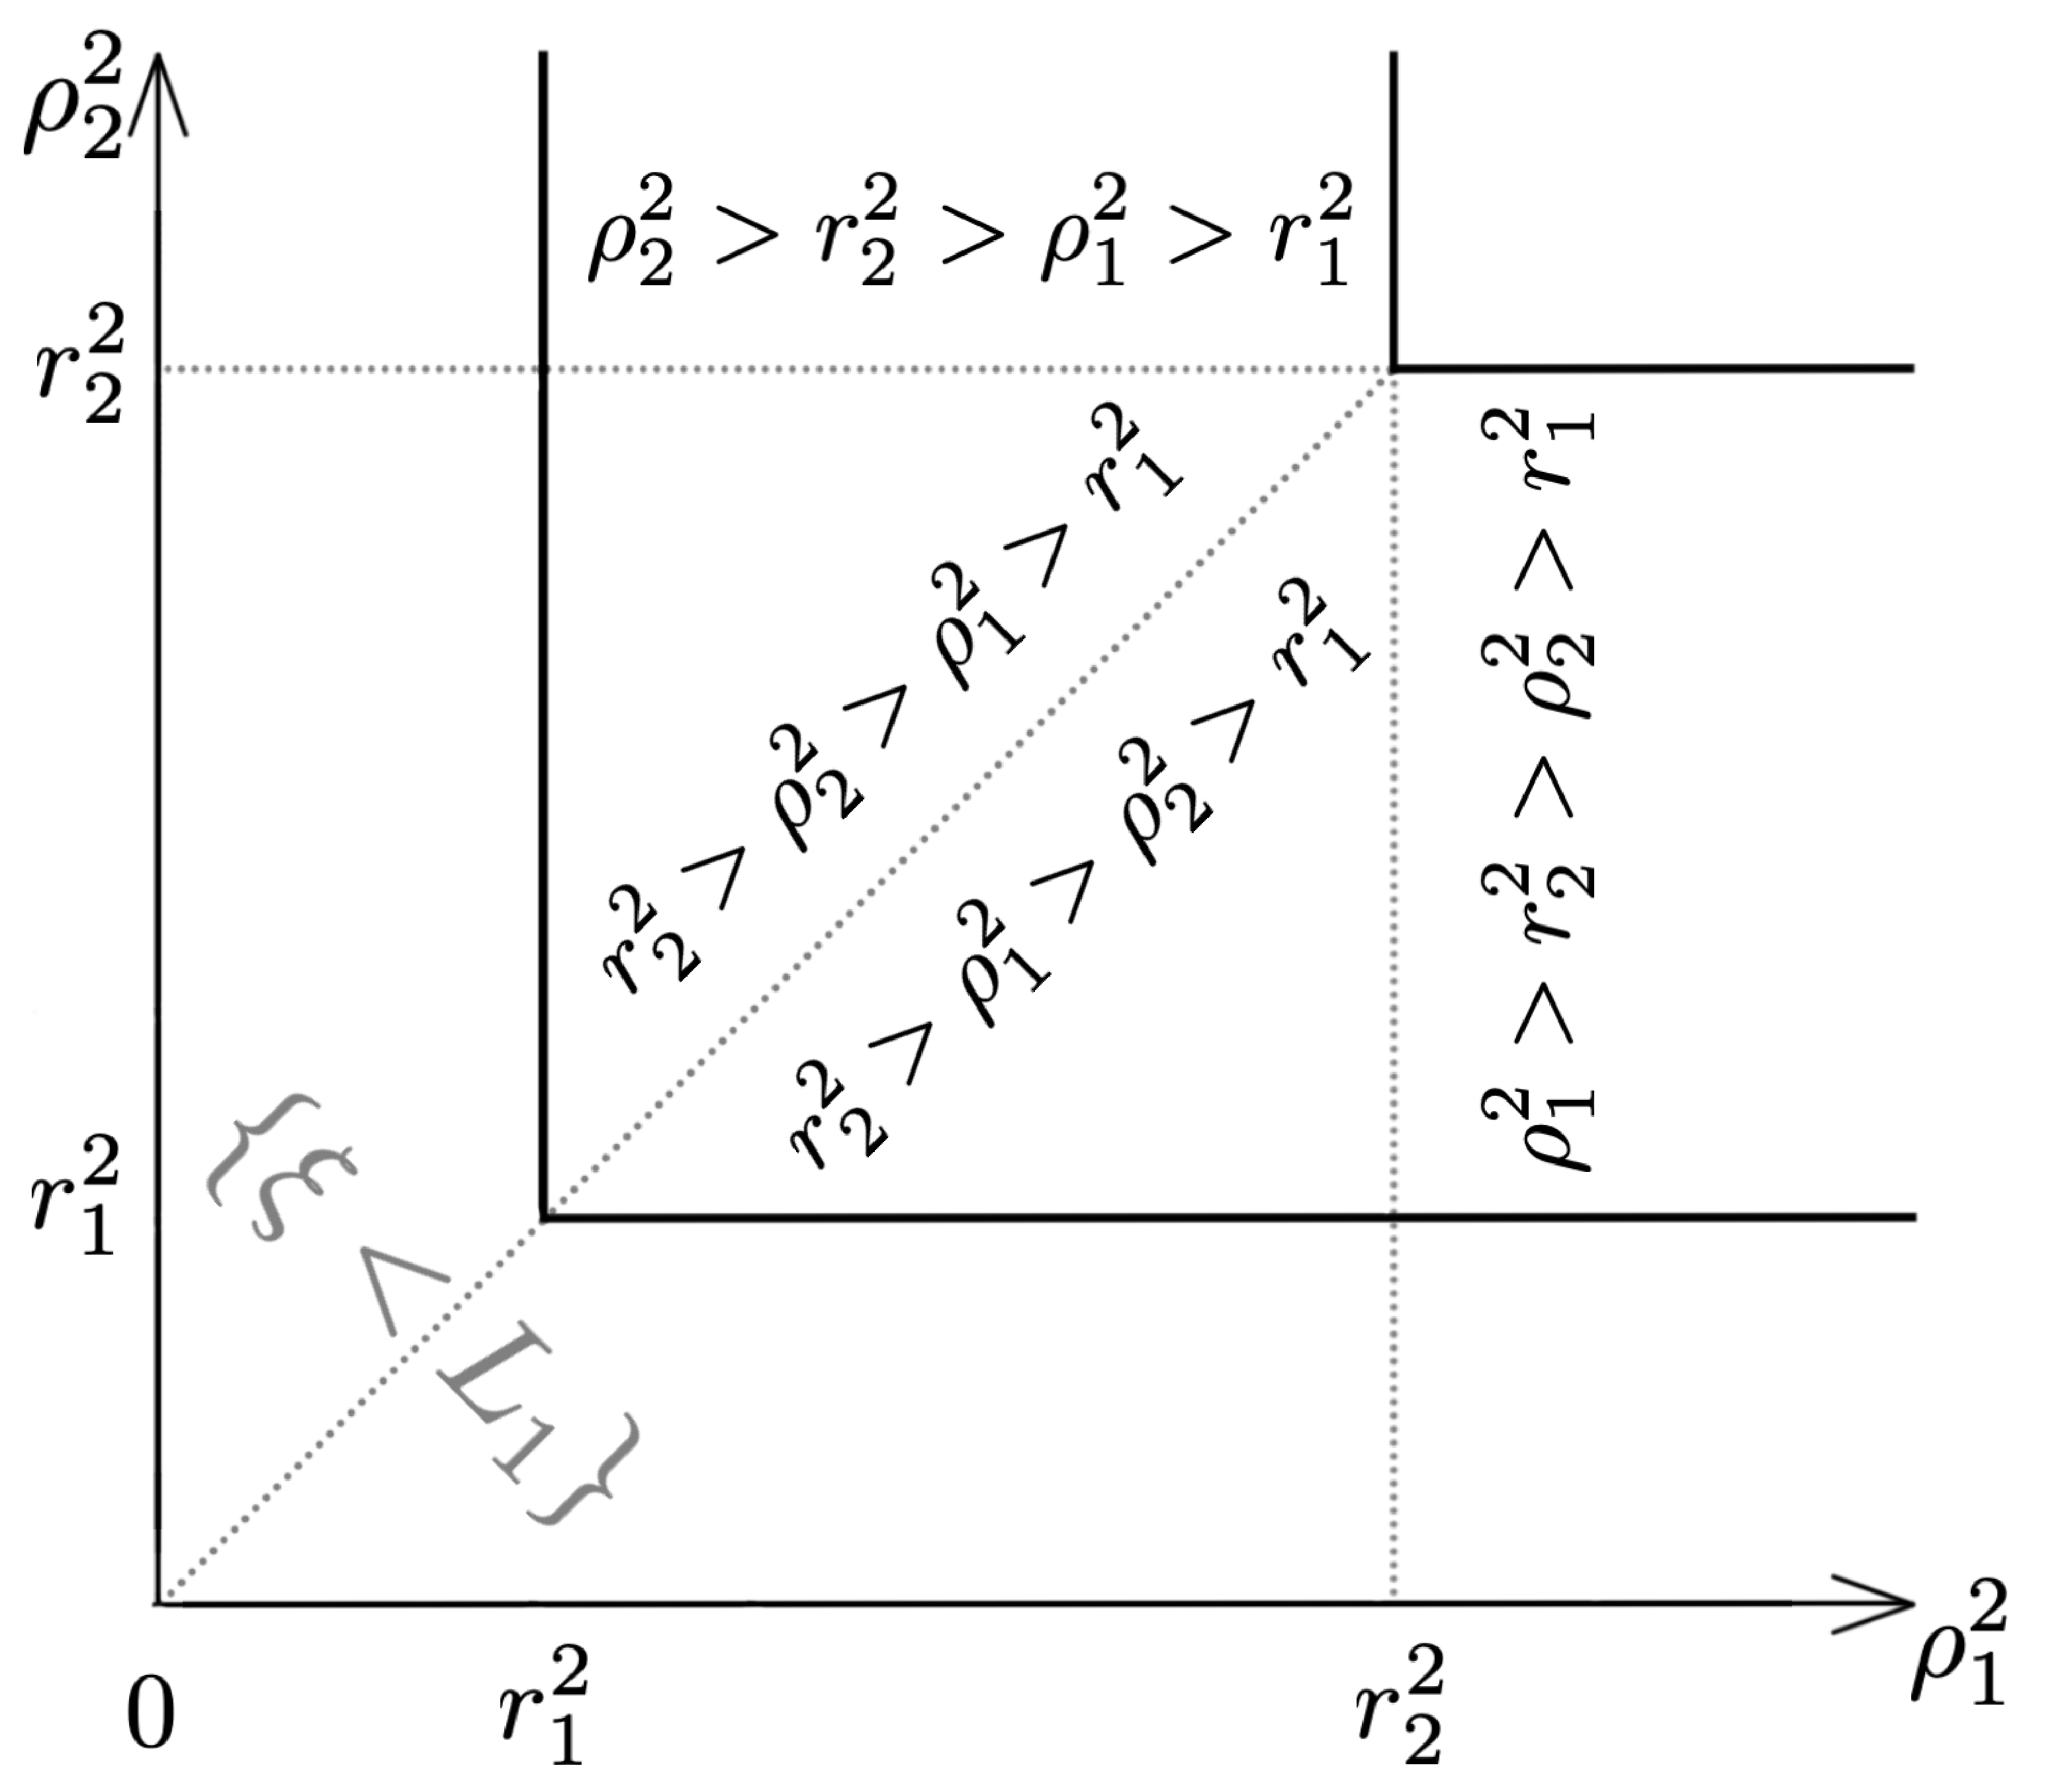
\includegraphics[width=6cm]{images/ch4/section3_circular/sect3_xiL1_subdivision.pdf}
    \caption{Разбиение области $\left\{\xi > L_1\right\}$.}
    \label{fig:pt10:_xiL1_subdivision}
\end{figure}

%Область, соответствующая случаю $B_2$, ограничивается координатными линиями $r_1^2 \leq \rho_1^2 \leq \rho_2^2 , r_1^2 \leq \rho_2^2 \leq \rho_2^2$. 
\subsection{Случай $r_2^2 > \rho_1^2 > \rho_2^2 > r_1^2$}\label{sec:ch5/sec7/sub1}
Траектория в области $\Omega_1$ касается окружности радиуса $\rho_1 < r_2$, а в области $\Omega_2$ --- окружности радиуса $r_1 < \rho_2$. Проекция бильярдной траектории заметает область $\widetilde{\Omega} = (\Omega_1 \setminus B_{\rho_1}) \cup (\Omega_2 \setminus B_{\rho_2})$, где $B_r$ обозначает диск радиуса $r$ с радиусом в нуле. Область $\widetilde{\Omega}$ изображена на рис. \ref{fig:pt10:_B2_domain_1}. Пунктиром изображена дуга $EF$ окружности радиуса $r_1$. 
\begin{figure}[!htb]
\minipage{0.5\textwidth}
\centering
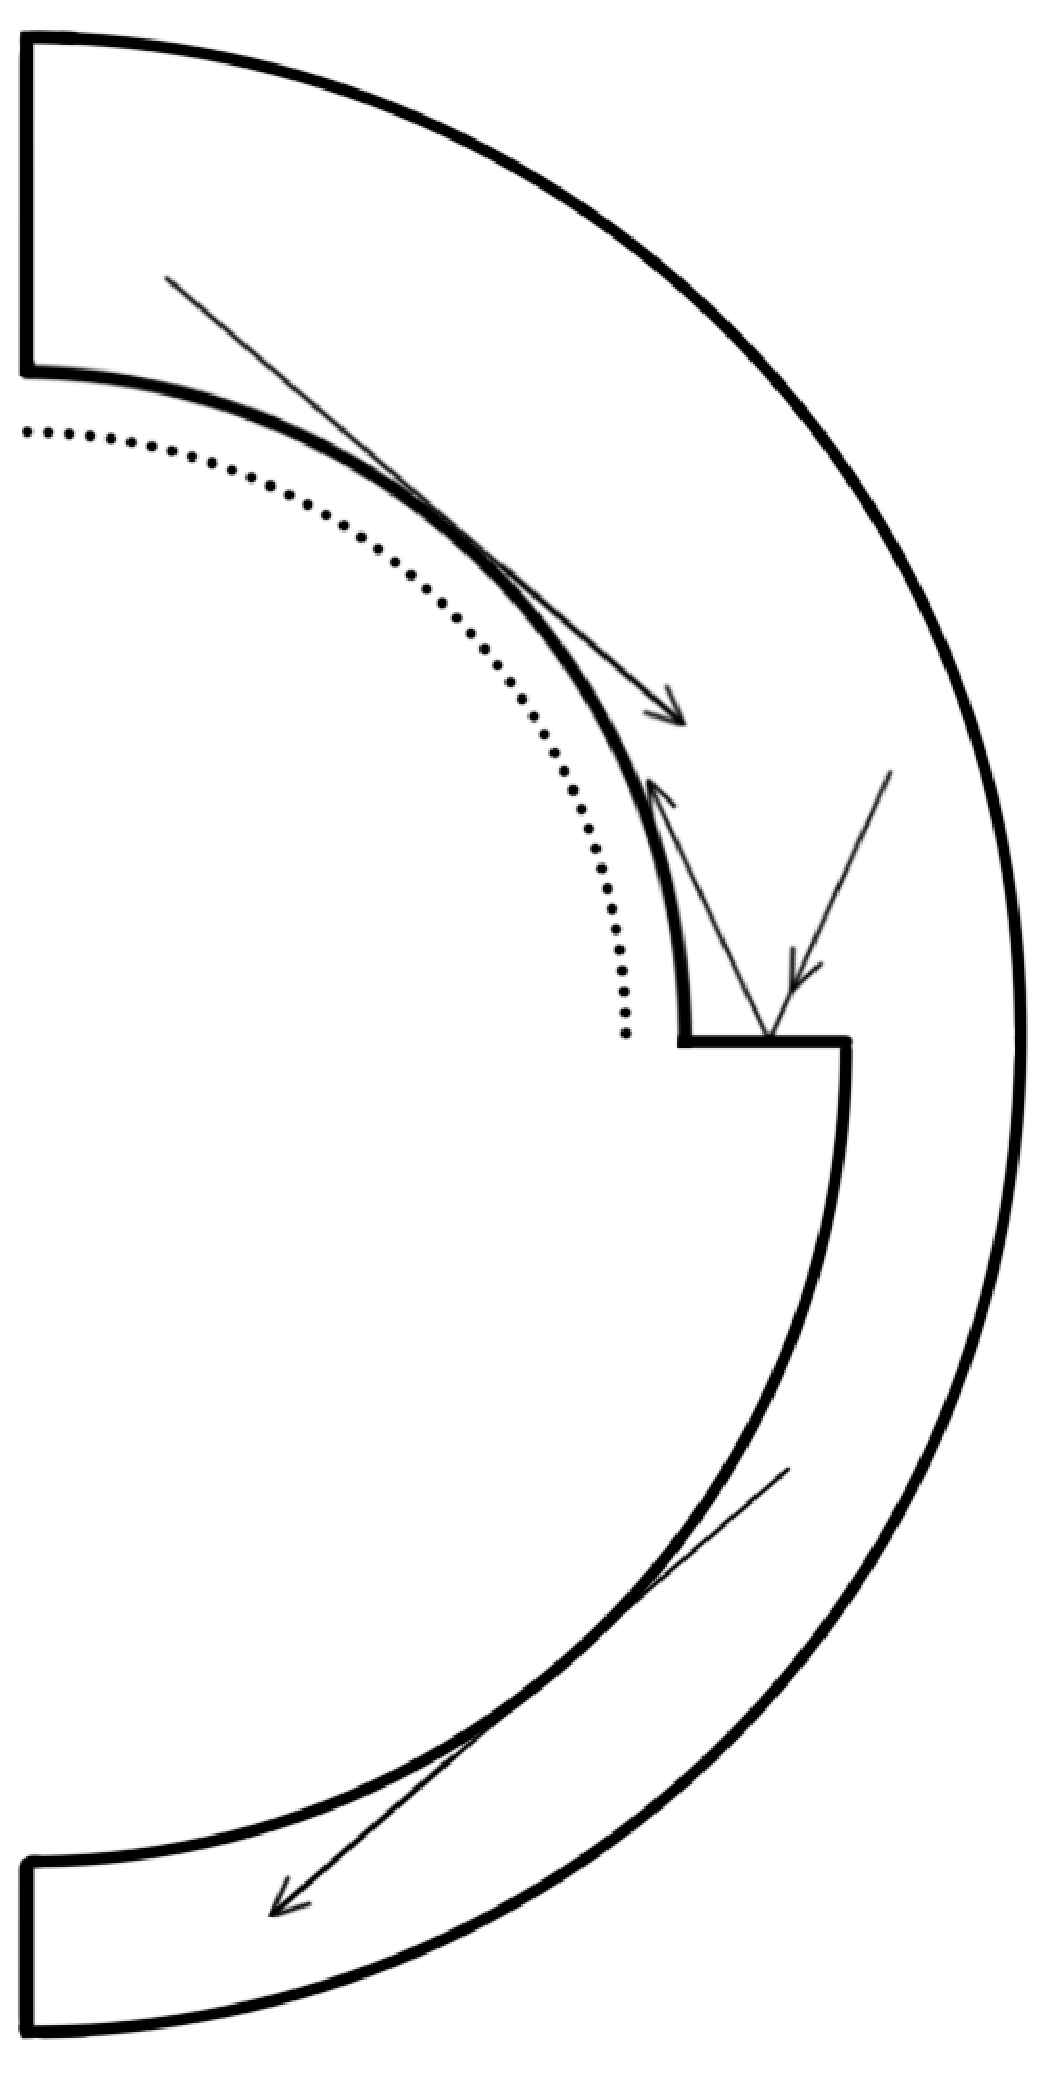
\includegraphics[width=2cm]{images/ch4/section3_circular/atoms/sect3_B2_domain_1.pdf}
    \caption{Область, заметаемая траекторией для случая $\xi > L_1$ при $r_2^2 > \rho_1^2 > \rho_2^2 > r_1^2$.}
    \label{fig:pt10:_B2_domain_1}
\endminipage\hfill
\minipage{0.5\textwidth}
\centering
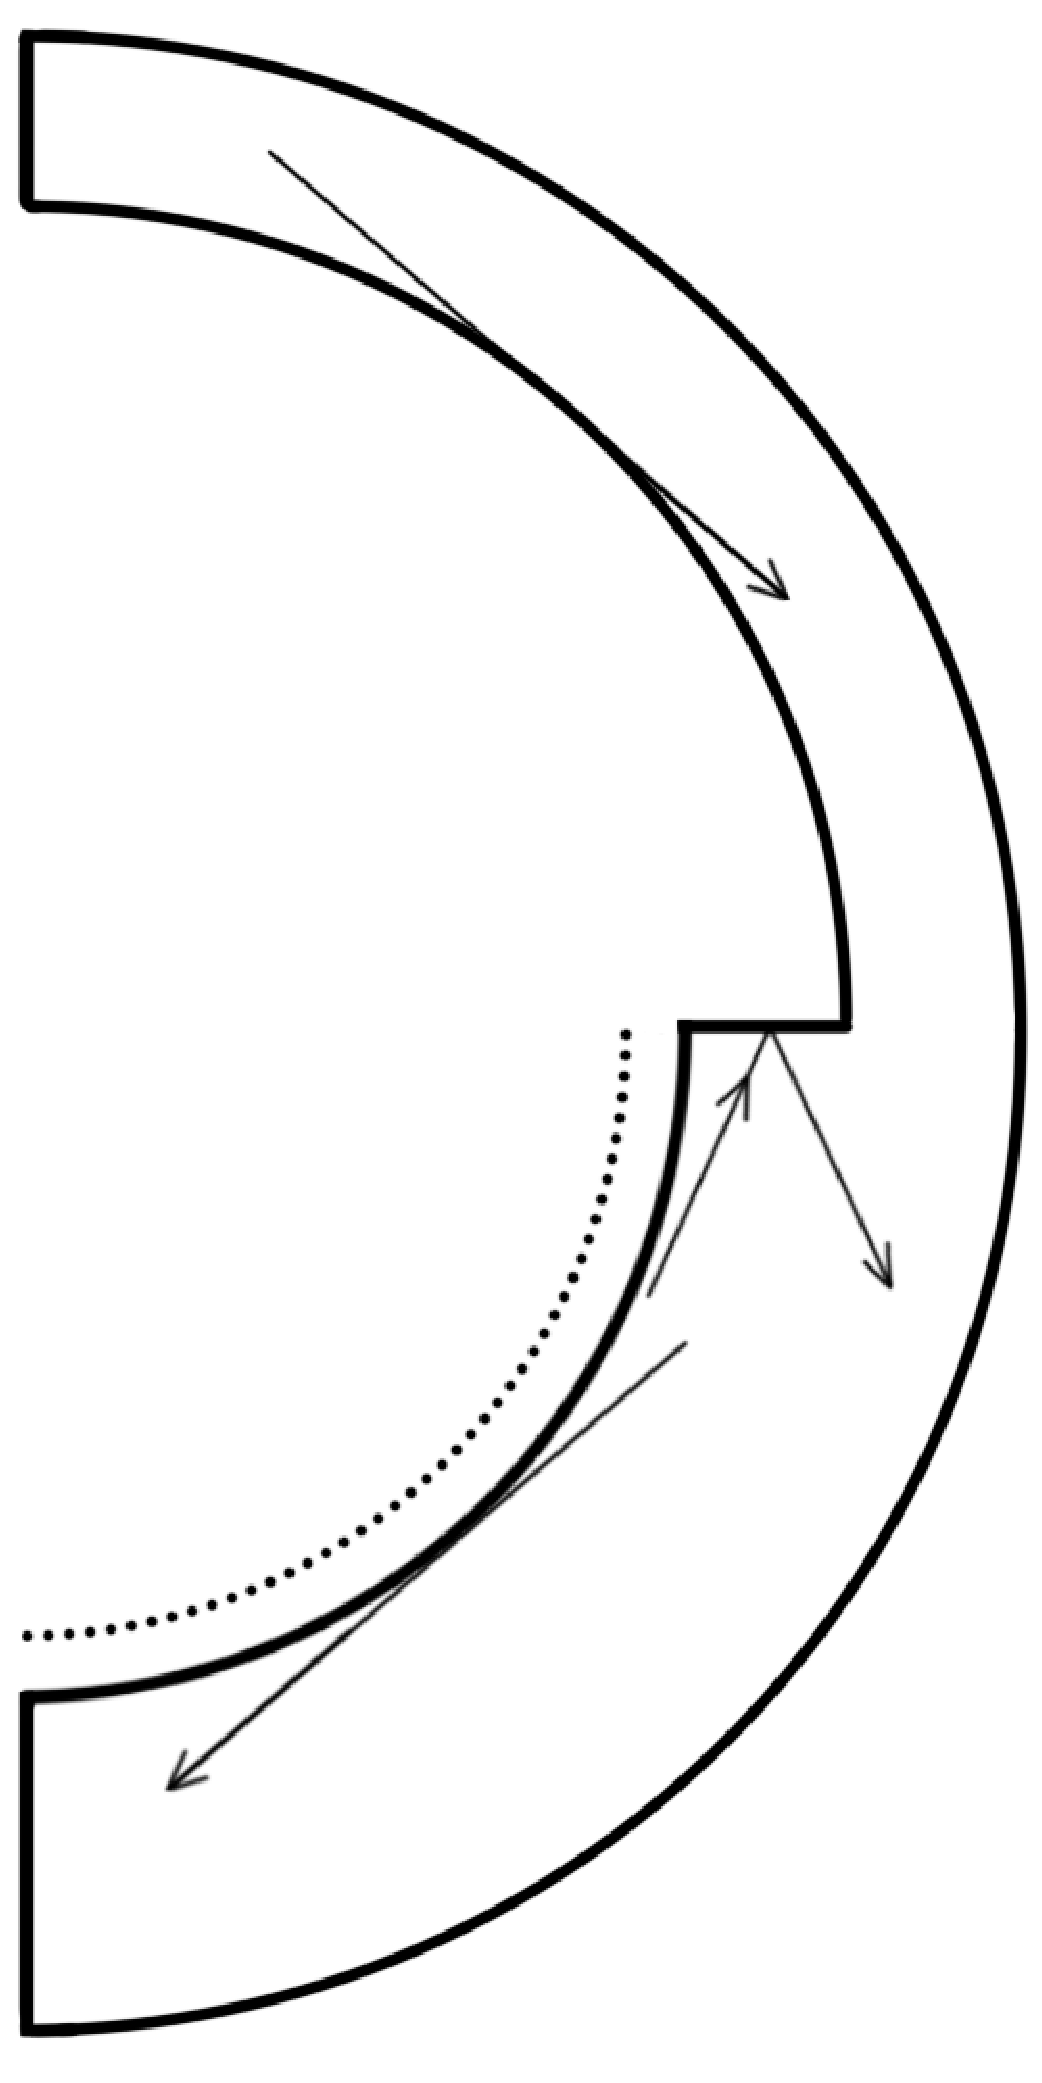
\includegraphics[width=2cm]{images/ch4/section3_circular/atoms/sect3_B2_domain_2.pdf}
    \caption{Область, заметаемая траекторией для случая $\xi > L_1$ при $r_2^2 > \rho_2^2 > \rho_1^2 > r_1^2$.}
        \label{fig:pt10:_B2_domain_2}
\endminipage\hfill
\end{figure}

Определим векторы скоростей $v_1, \ldots, v_4$ в соответствии с правилами \eqref{eq:foc_numeration_circle}. С каждым вектором скорости ассоциируем по одной из областей $\widetilde{\Omega}_1, \ldots, \widetilde{\Omega}_4$, каждая выглядит как показано на  рис. \ref{fig:pt10:_B2_domain_1}. 
Склейкой областей $\widetilde{\Omega}_1 \cup \widetilde{\Omega}_4$ по дугам, проектирующимся на дуги граничных окружностей $\widetilde{\Omega}$, получим сферу с тремя дырками. Аналогично для склейки $\widetilde{\Omega}_2 \cup \widetilde{\Omega}_3$. Склейкой двух таких сфер по общим границам дырок, которые проектируются на прямолинейные граничные отрезки $\widetilde{\Omega}$, получим поверхность $\Xi=\const$, которая является сферой с двумя ручками. 

\subsection{Случай  $r_2^2 > \rho_2^2 > \rho_1^2 > r_1^2$}\label{sec:ch5/sec7/sub2}
Данный случай рассматривается аналогично предыдущему пункту. Заметаемая точкой область $\widetilde{\Omega}$ изображена на рис. \ref{fig:pt10:_B2_domain_2}, дальнейшие рассуждения повторяют пункт \ref{sec:ch5/sec7/sub1}. Поверхность $\Xi = \const$ также является сферой с двумя ручками.

\subsection{Случай  $\rho_2^2 > r_2^2 > \rho_1^2 > r_1^2$ и случай $\rho_1^2 > r_2^2 > \rho_2^2 > r_1^2$}\label{sec:ch5/sec7/sub3}
В обоих случаях  точка при движении заметает область $\widetilde{\Omega}$, которая ограничивается дугами двух окружностей и отрезками двух прямых (см. рис. \ref{fig:pt10:_B3_domain}, \ref{fig:pt10:_B4_domain}).
\begin{figure}[!htb]
\minipage{0.5\textwidth}
\centering
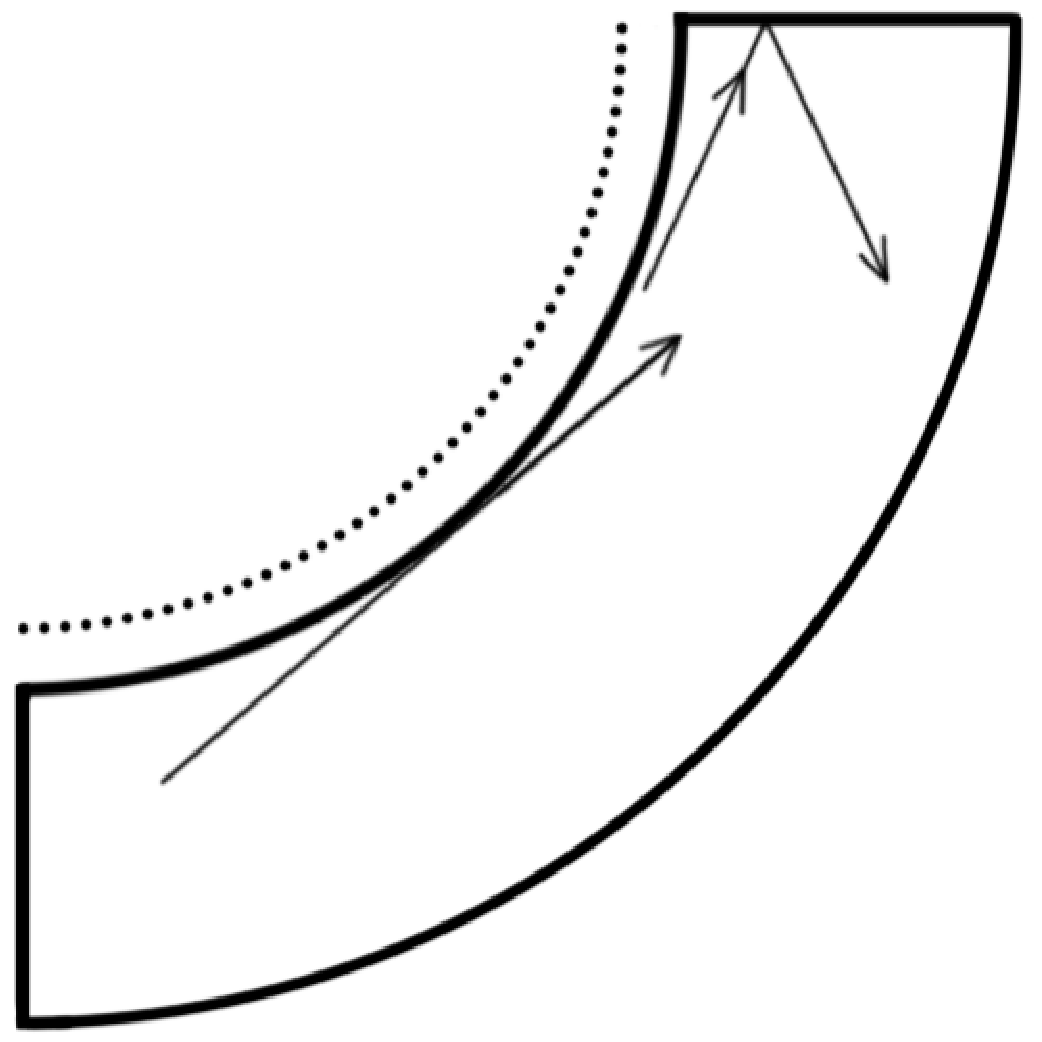
\includegraphics[width=2cm]{images/ch4/section3_circular/atoms/sect3_B3_domain.pdf}
    \caption{Область, заметаемая траекторией для случая $\rho_2^2 > r_2^2 > \rho_1^2 > r_1^2$.}
    \label{fig:pt10:_B3_domain}
\endminipage\hfill
\minipage{0.5\textwidth}
\centering
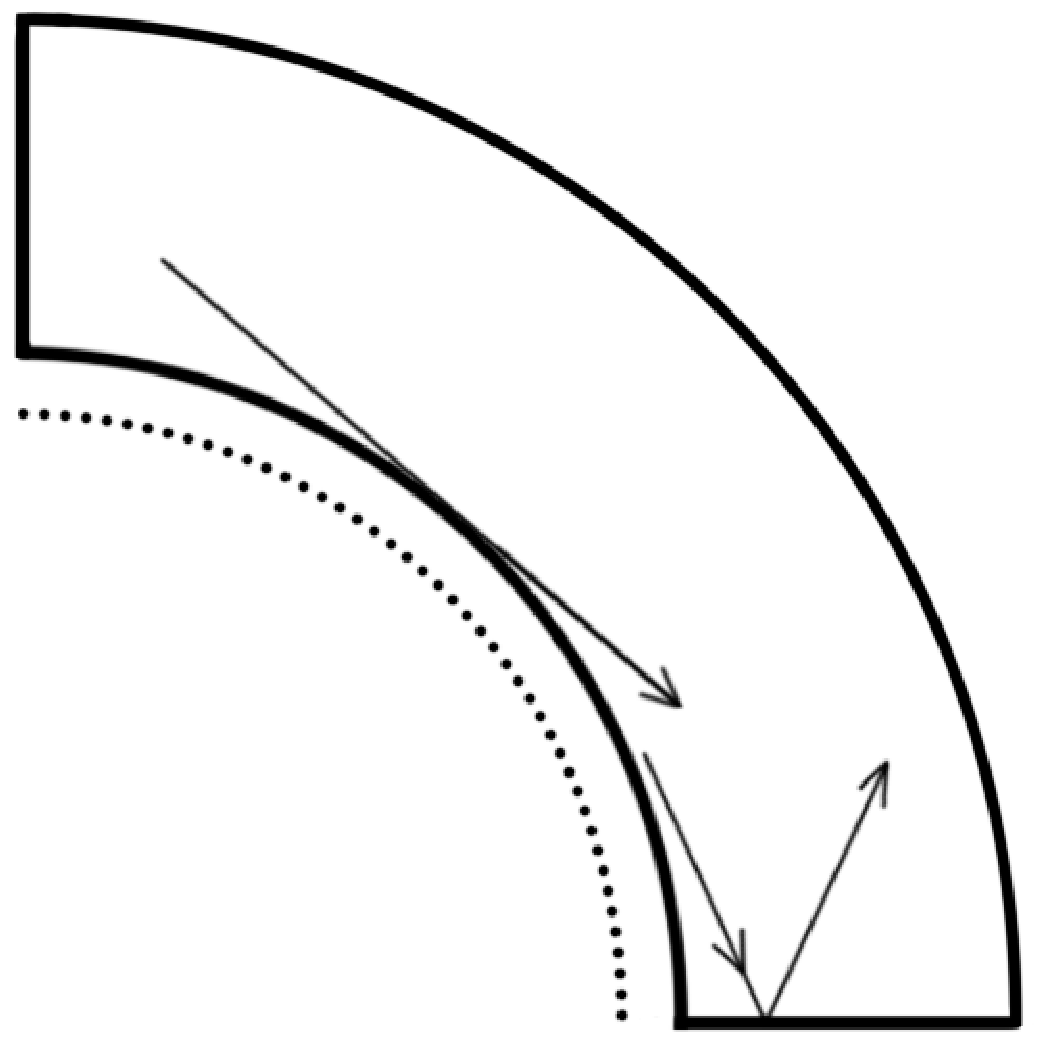
\includegraphics[width=2cm]{images/ch4/section3_circular/atoms/sect3_B4_domain.pdf}
    \caption{Область, заметаемая траекторией для случая $\rho_1^2 > r_2^2 > \rho_2^2 > r_1^2$.}
        \label{fig:pt10:_B4_domain}
\endminipage\hfill
\end{figure}

Определим векторы $v_1, \ldots, v_4$ в соответствии с правилами \eqref{eq:foc_numeration_circle}, области $\widetilde{\Omega}_1, \ldots, \widetilde{\Omega}_4$ зададим так же, как и ранее.
Склейкой областей $\widetilde{\Omega}_1 \cup \widetilde{\Omega}_4$ по дугам, проектирующимся на дуги граничных окружностей $\widetilde{\Omega}$, получим сферу с двумя дырками. Аналогично для склейки $\widetilde{\Omega}_2 \cup \widetilde{\Omega}_3$. Склейкой двух таких сфер по общим границам дырок, получим поверхность $\Xi = \const$, которая является тором.


\section{Особые поверхности для случая $\left\{ \xi < L_1 \right\}$}\label{sec:ch5/sec8}
Для простоты ограничимся случаем  $n_1^2 < n_2^2$. 
На рис. \ref{fig:pt10:_C_kPrime_definitions} серые клинья с одной стороны ограничиваются кривыми семейства $III$, а с другой --- кривыми семейства $IV$, см. \eqref{eq:IVdef}.

Перемещаясь вдоль прямой $L$, мы меняем значение интеграла $\Xi$; в точках пересечения прямой $L$ с кривыми  из семейств $II$, $III$ или $IV$ поверхность $S_\Xi$ испытывает перестройку.
%, см. рис. 
%\begin{figure}[!htb]
%\centering
%\includegraphics[scale=0.12]{images/ch4/section3_circular/atoms/bifurcations/lines_families.pdf}
%    \caption{Область, заметаемая траекторией для случая $B_3$.}
%    \label{fig:pt10:_B3_domain}
%\end{figure}

Заметим, что не имеет значения, какую  именно кривую мы пересекаем: важно только семейство кривых, к которому она относится. Поверхность $S_\Xi$ будет испытывать одну и ту же бифуркацию при пересечении любой кривой, относящейся к данному семейству.
 
 \subsection{Семейство $II$}
 В момент пересечения кривой $II_m$ область $\widetilde{\Omega}$, изображенная на рис.     \ref{fig:pt10:_big_domain_transformed}, меняется следующим образом:
 к ее левой части подклеивается новый семиугольник, см. рис.     \ref{fig:pt10:_terminal_min_domain_transformed}.
 \begin{figure}[!htb]
\minipage{0.33\textwidth}
\centering
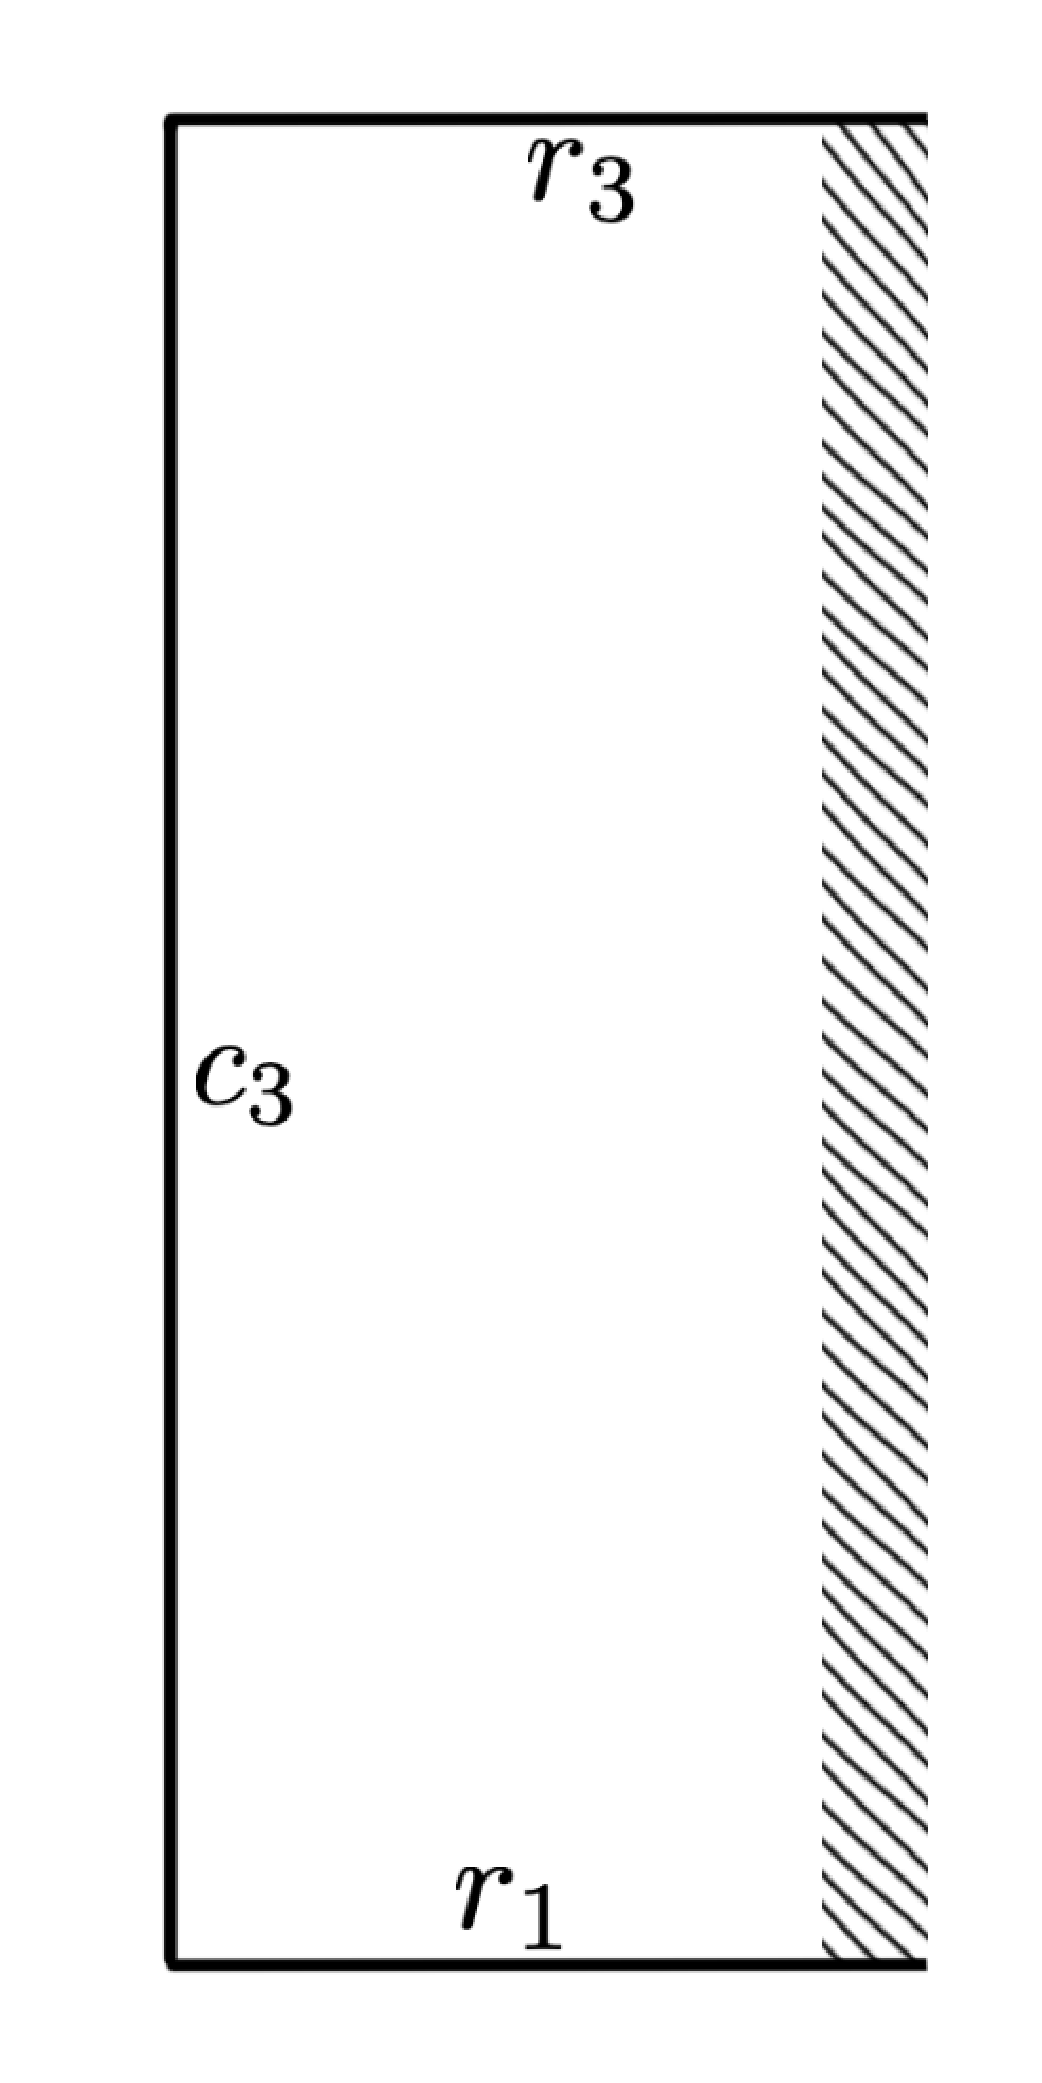
\includegraphics[scale=0.12]{images/ch4/section3_circular/atoms/II/before/before_page_segment.pdf}
    \caption{До бифуркации.}
        \label{fig:pt10:_II_before_segment}
\endminipage\hfill
\minipage{0.33\textwidth}
\centering
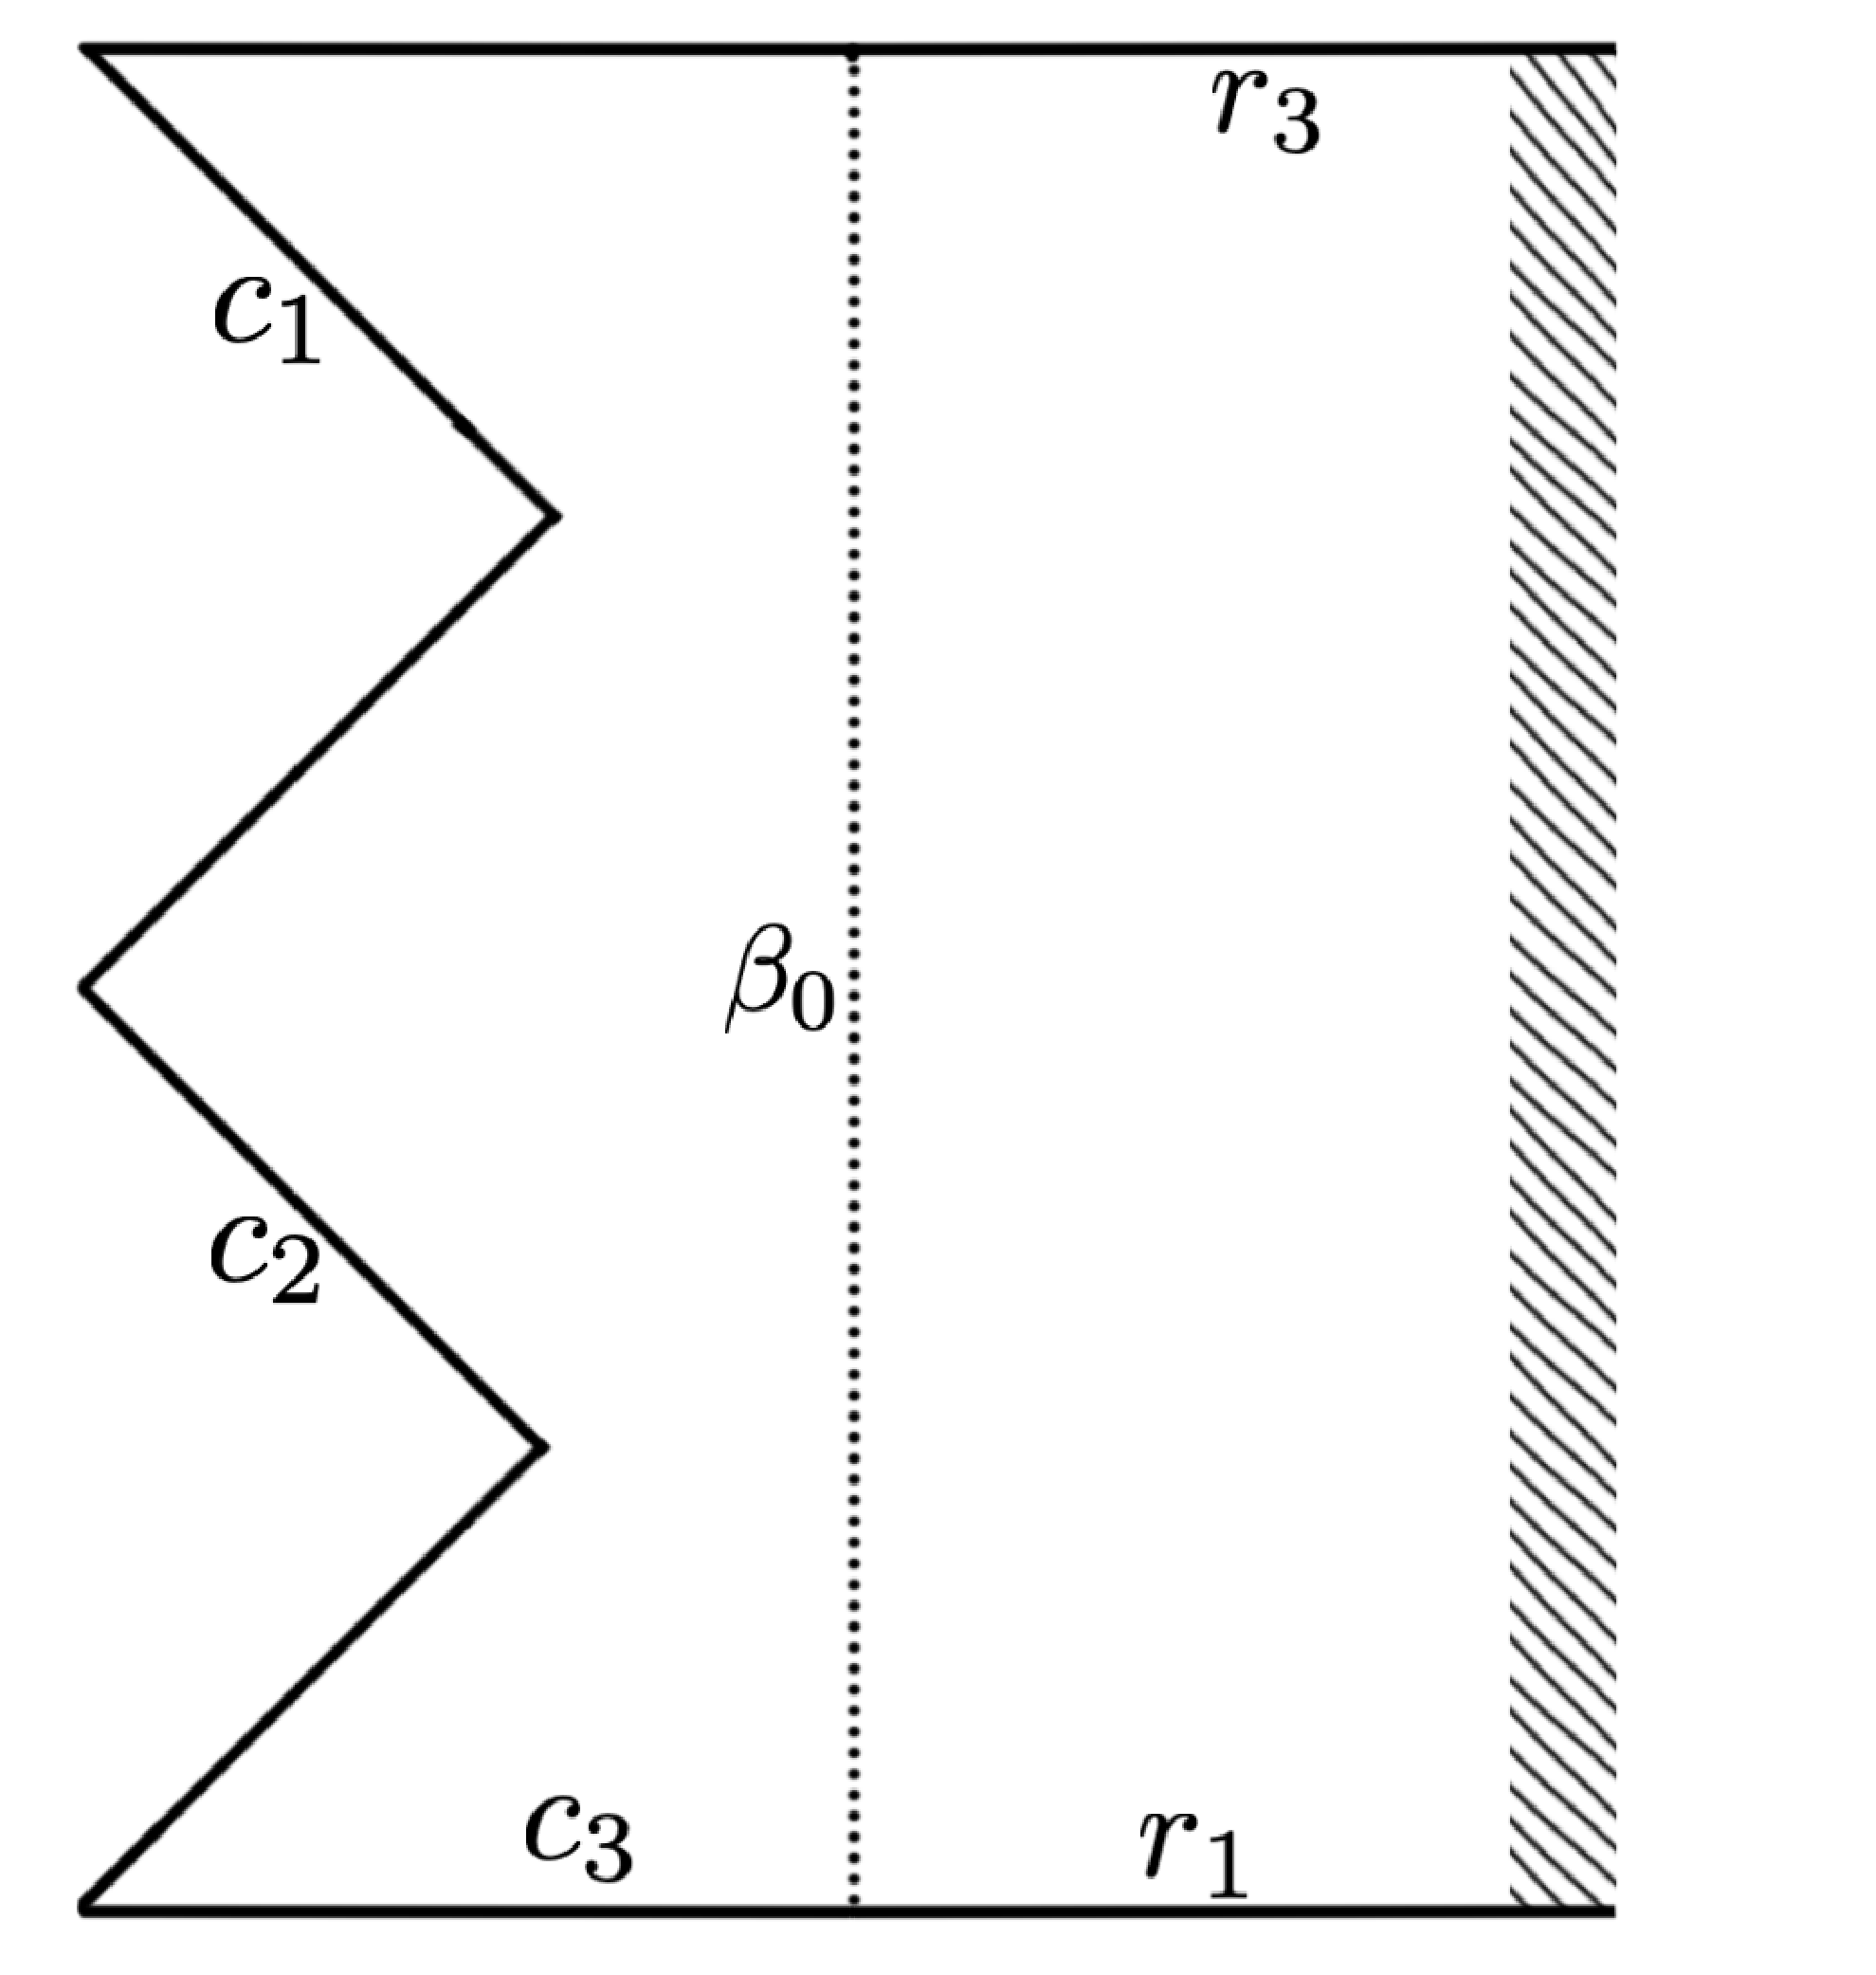
\includegraphics[scale=0.11]{images/ch4/section3_circular/atoms/II/bifurcation/page_segment.pdf}
    \caption{В момент бифуркации.}
    \label{fig:pt10:_II_page_segment}
\endminipage\hfill
\minipage{0.33\textwidth}
\centering
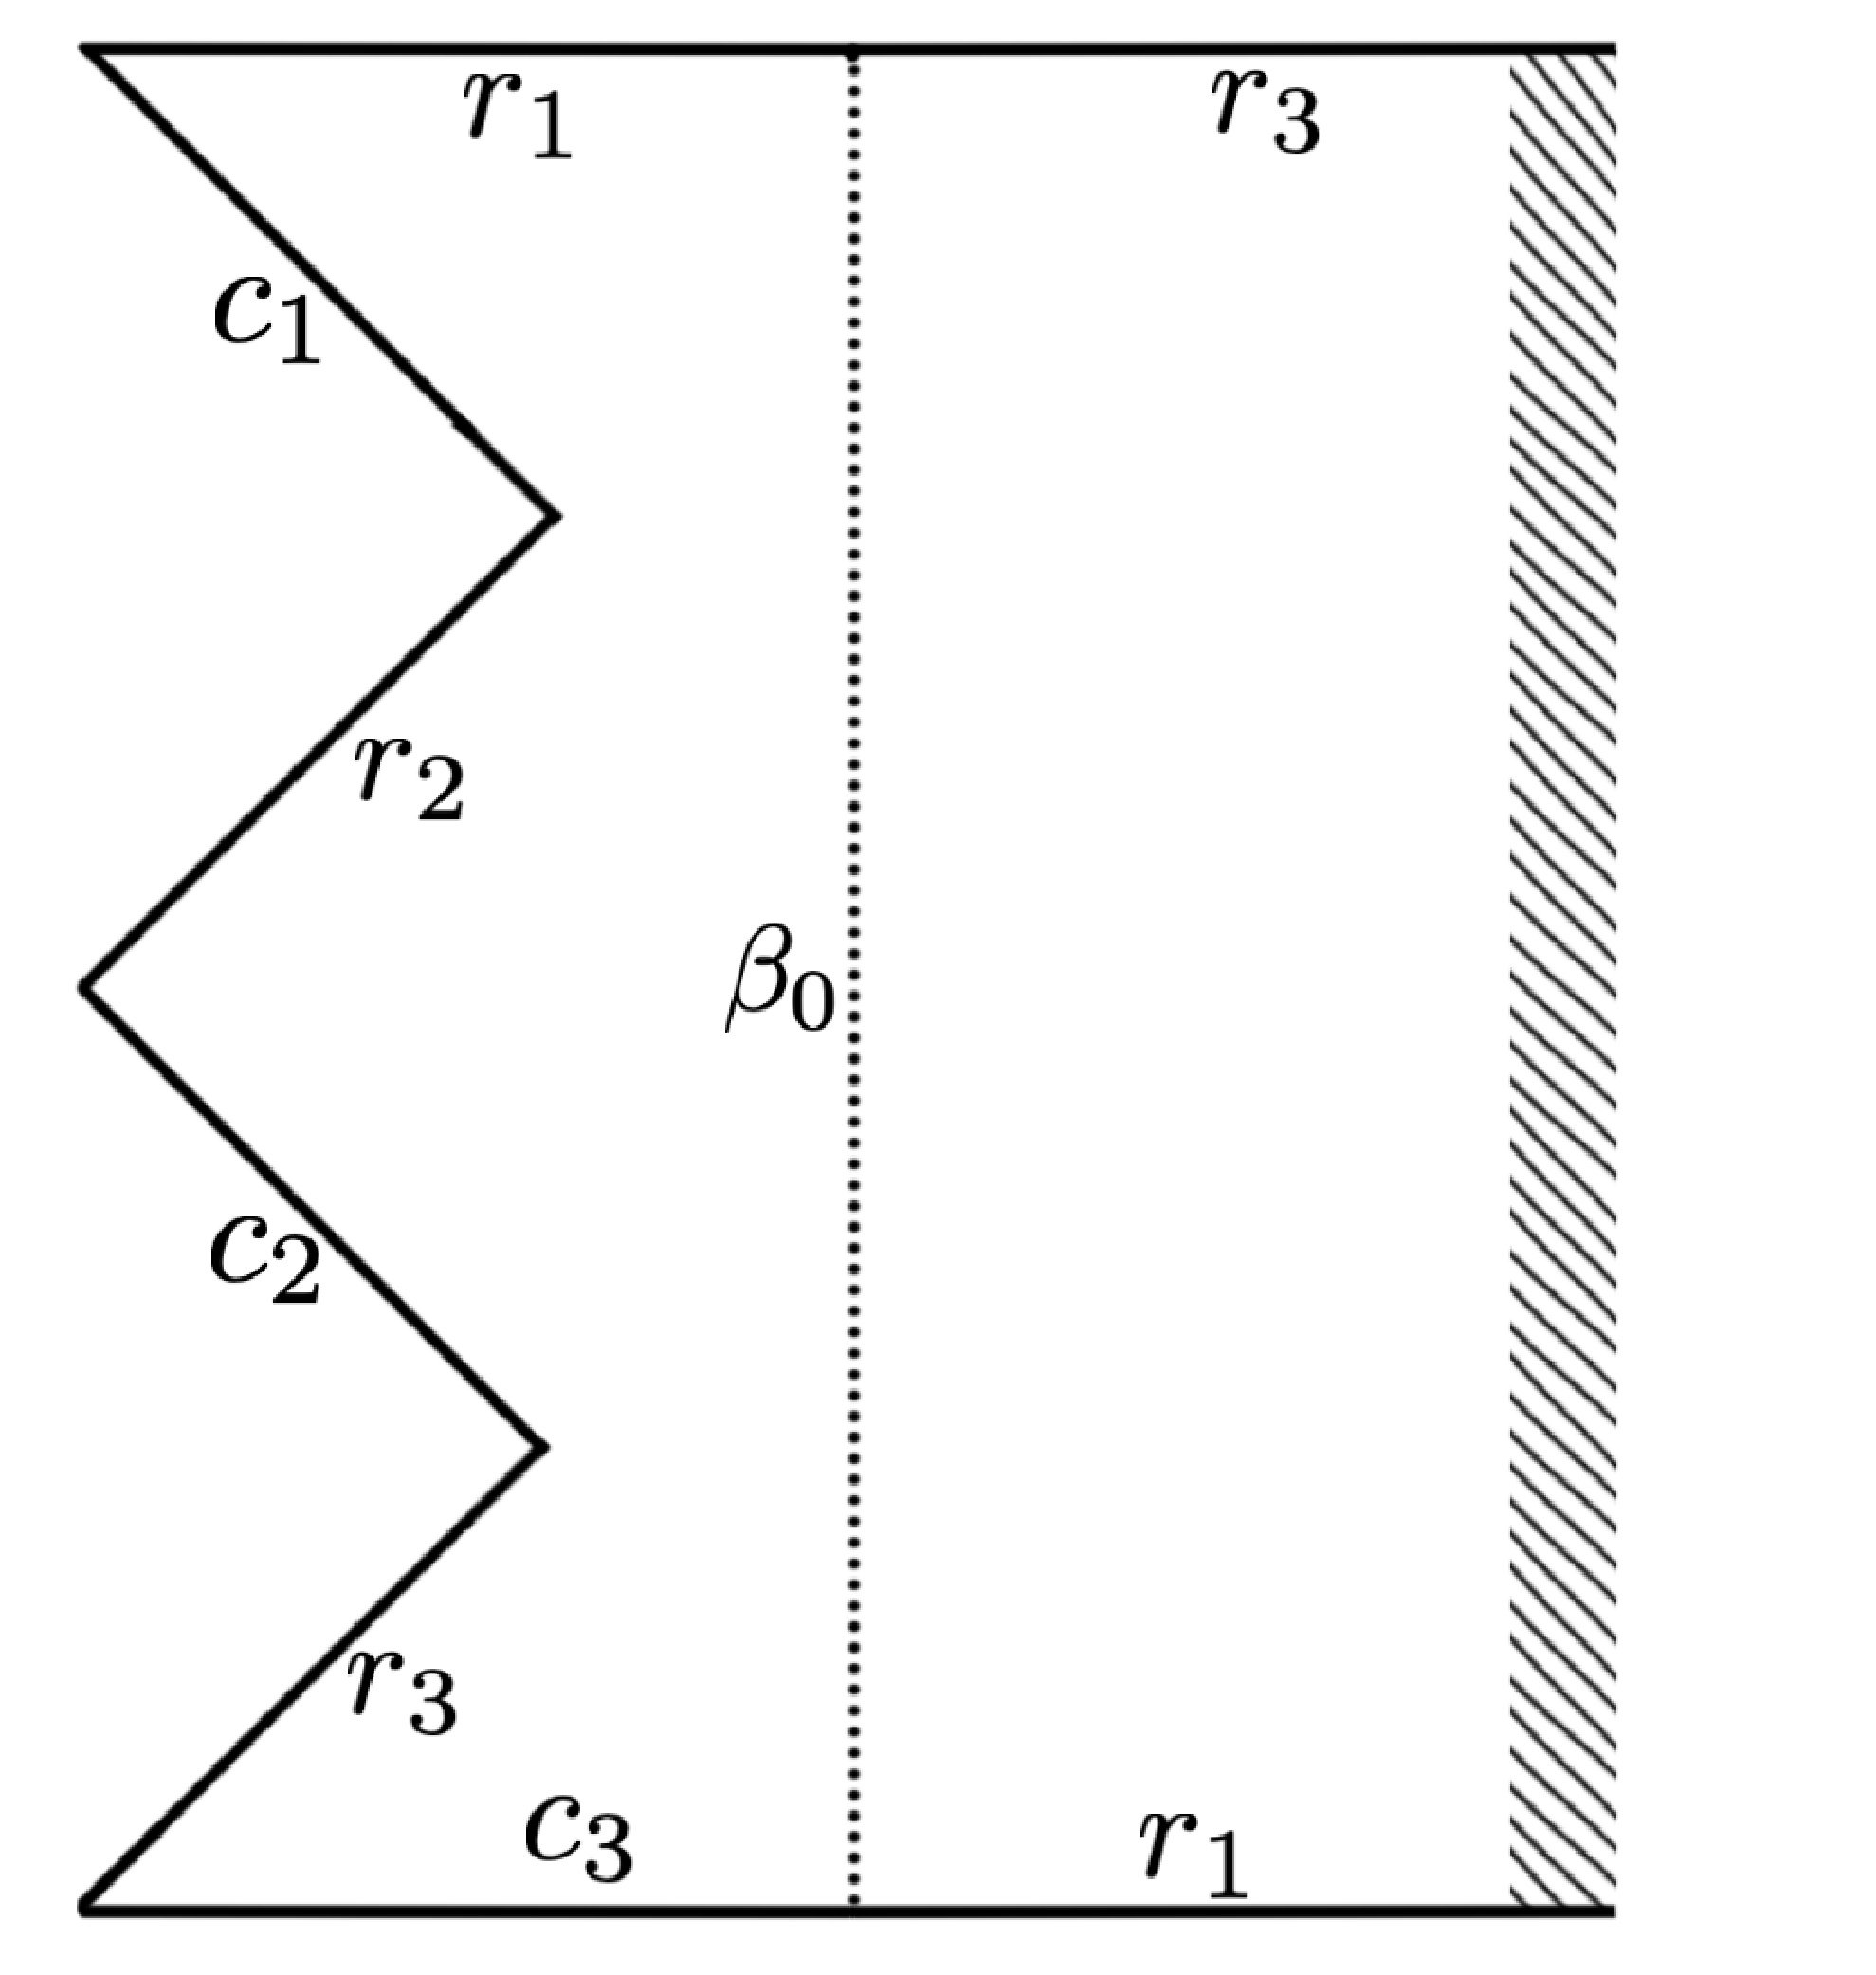
\includegraphics[scale=0.11]{images/ch4/section3_circular/atoms/II/after/page_segment.pdf}
    \caption{После бифуркации.}
    \label{fig:pt10:_II_after_page_segment}
\endminipage\hfill
\end{figure}

При этом оказывается, что правило \eqref{eq:foc_numeration_circle} на этом новом подклеенном семиугольнике не действует, так как для любой внутренней точки нового листа определены не четыре вектора скорости, а всего два: к общему центру окружностей или от него. Поэтому для каждой точки этого семиугольника на особой поверхности $S_\Xi$ заданы всего два прообраза. 

Типичная траектория на особой поверхности показана на рис.     \ref{fig:pt10:_II_trajectories_1}. Аналог докритической траектории изображен на рис.     \ref{fig:pt10:_II_before_trajectories}.
\begin{figure}[!htb]
\minipage{0.5\textwidth}
\centering
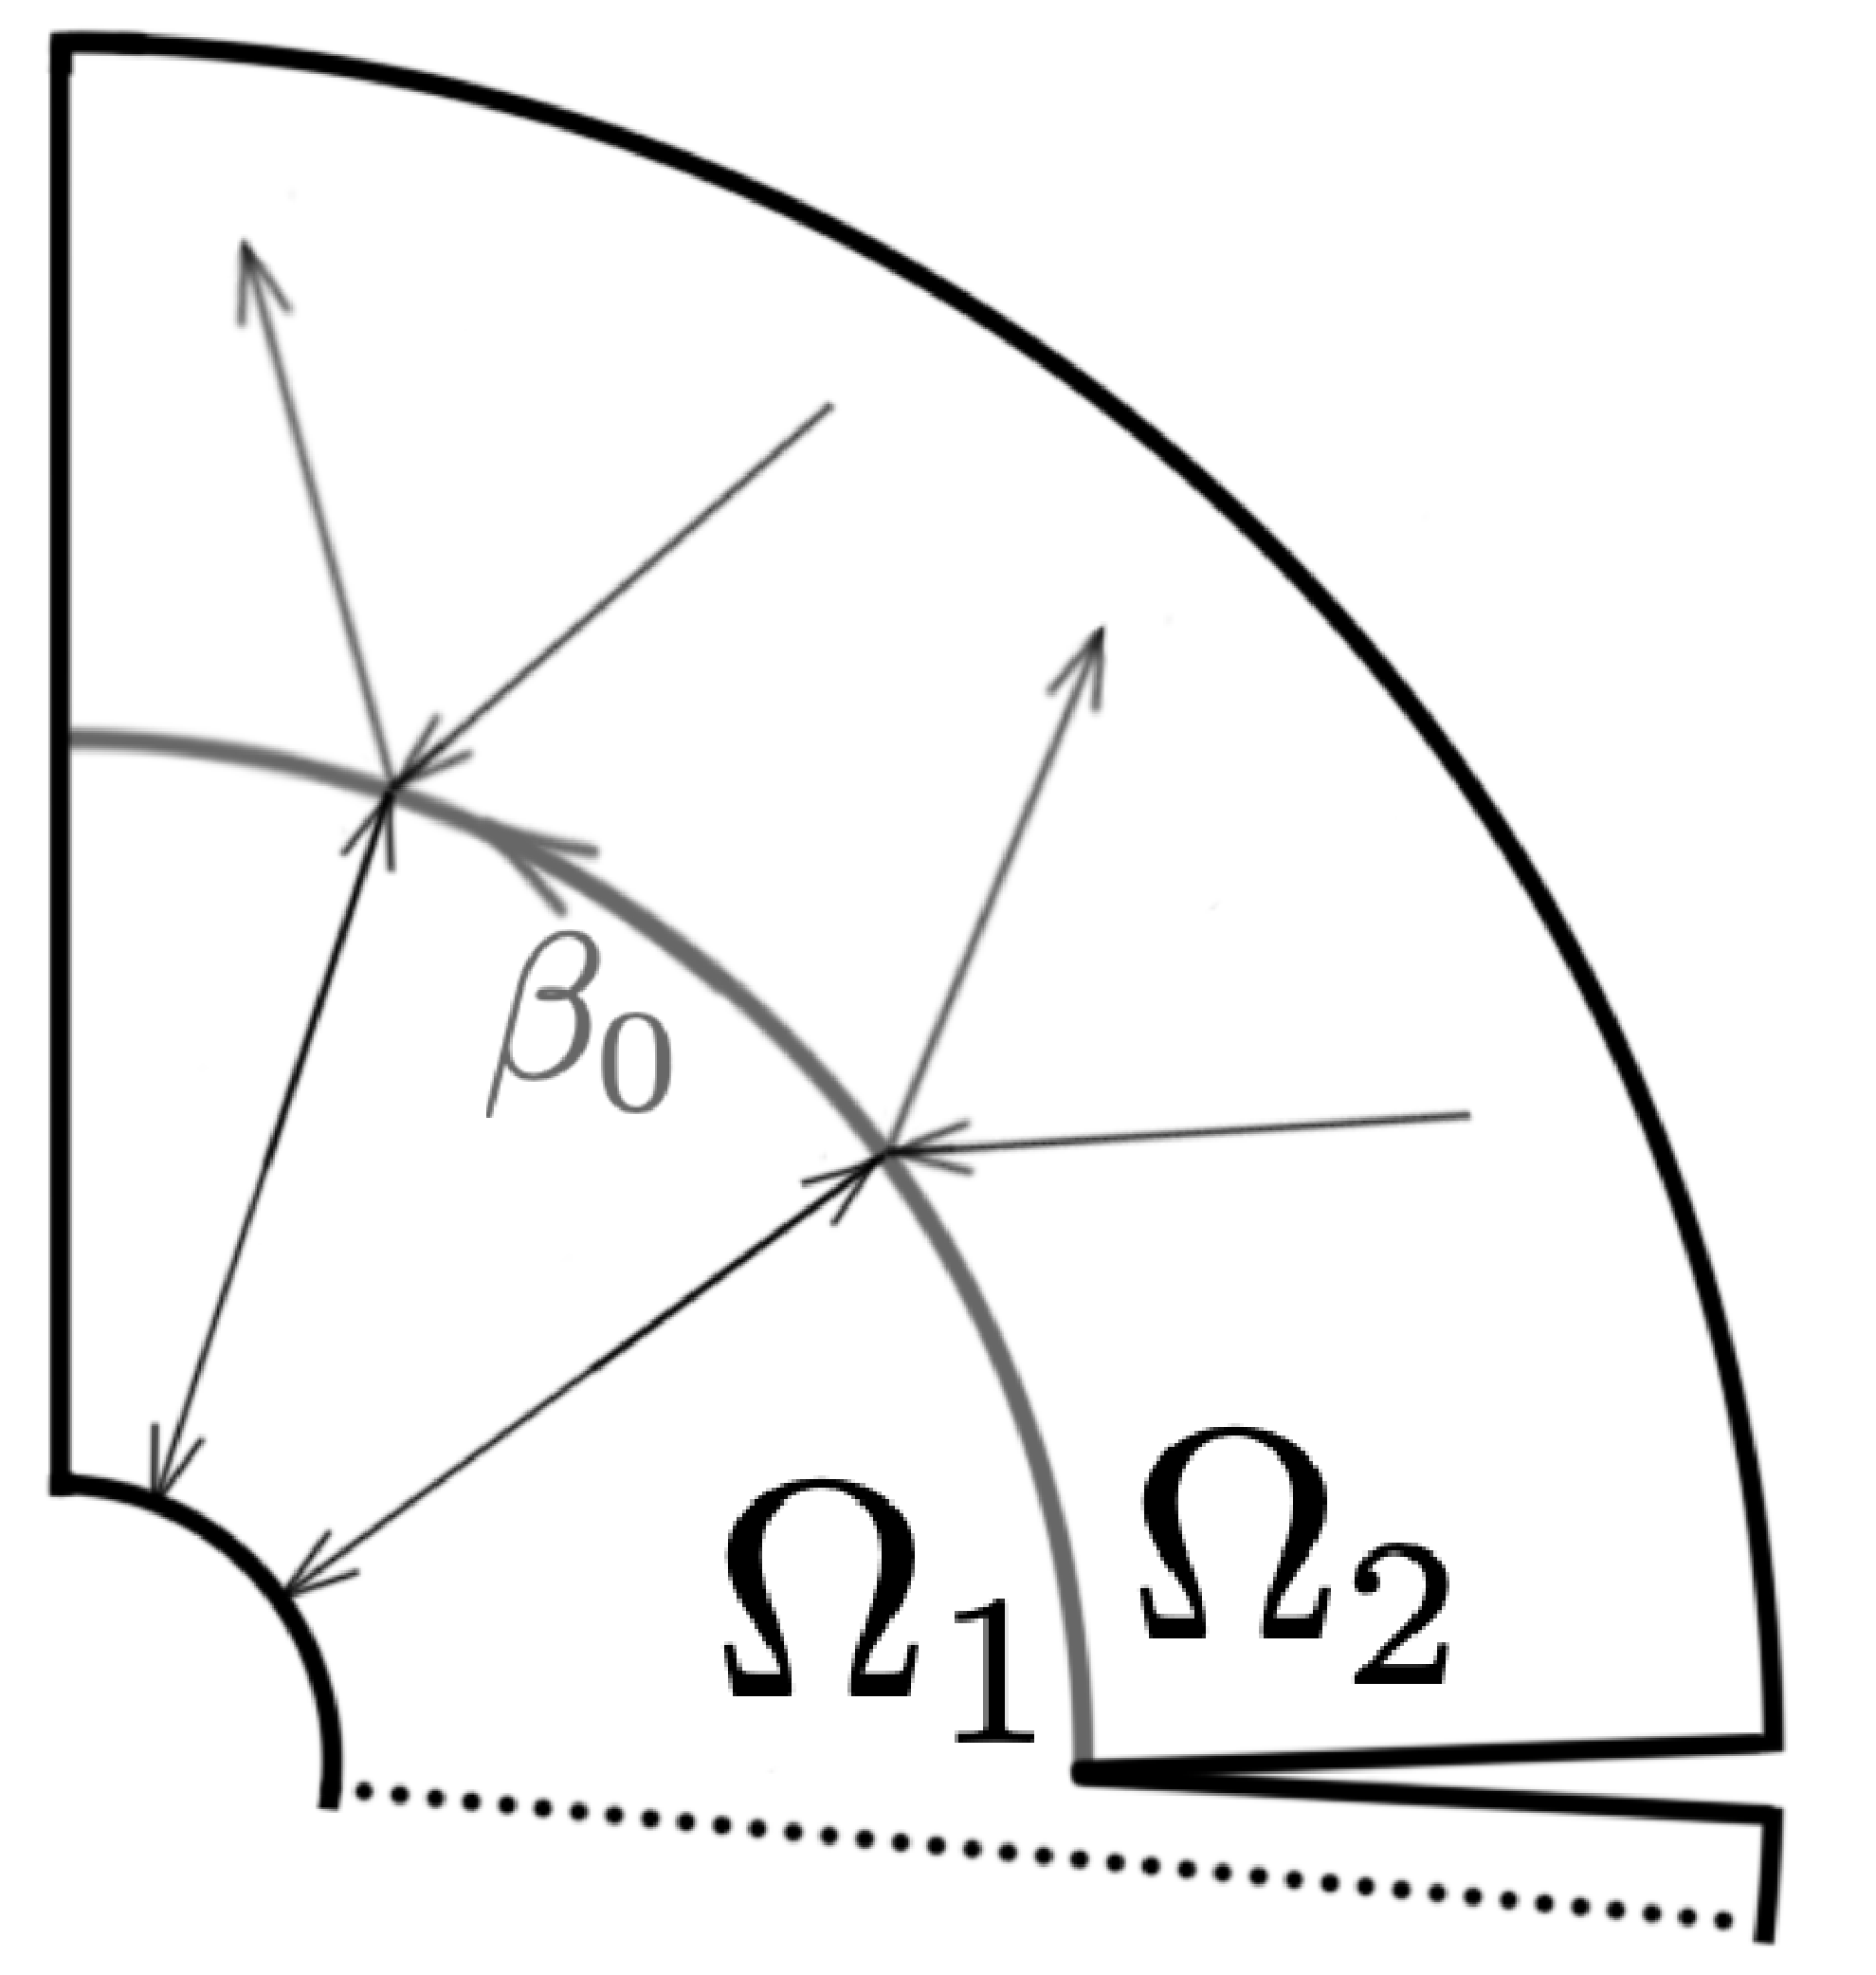
\includegraphics[scale=0.1]{images/ch4/section3_circular/atoms/II/bifurcation/trajectories_1.pdf}
    \caption{Пример траекторий в момент бифуркации.}
    \label{fig:pt10:_II_trajectories_1}
\endminipage\hfill
\minipage{0.5\textwidth}
\centering
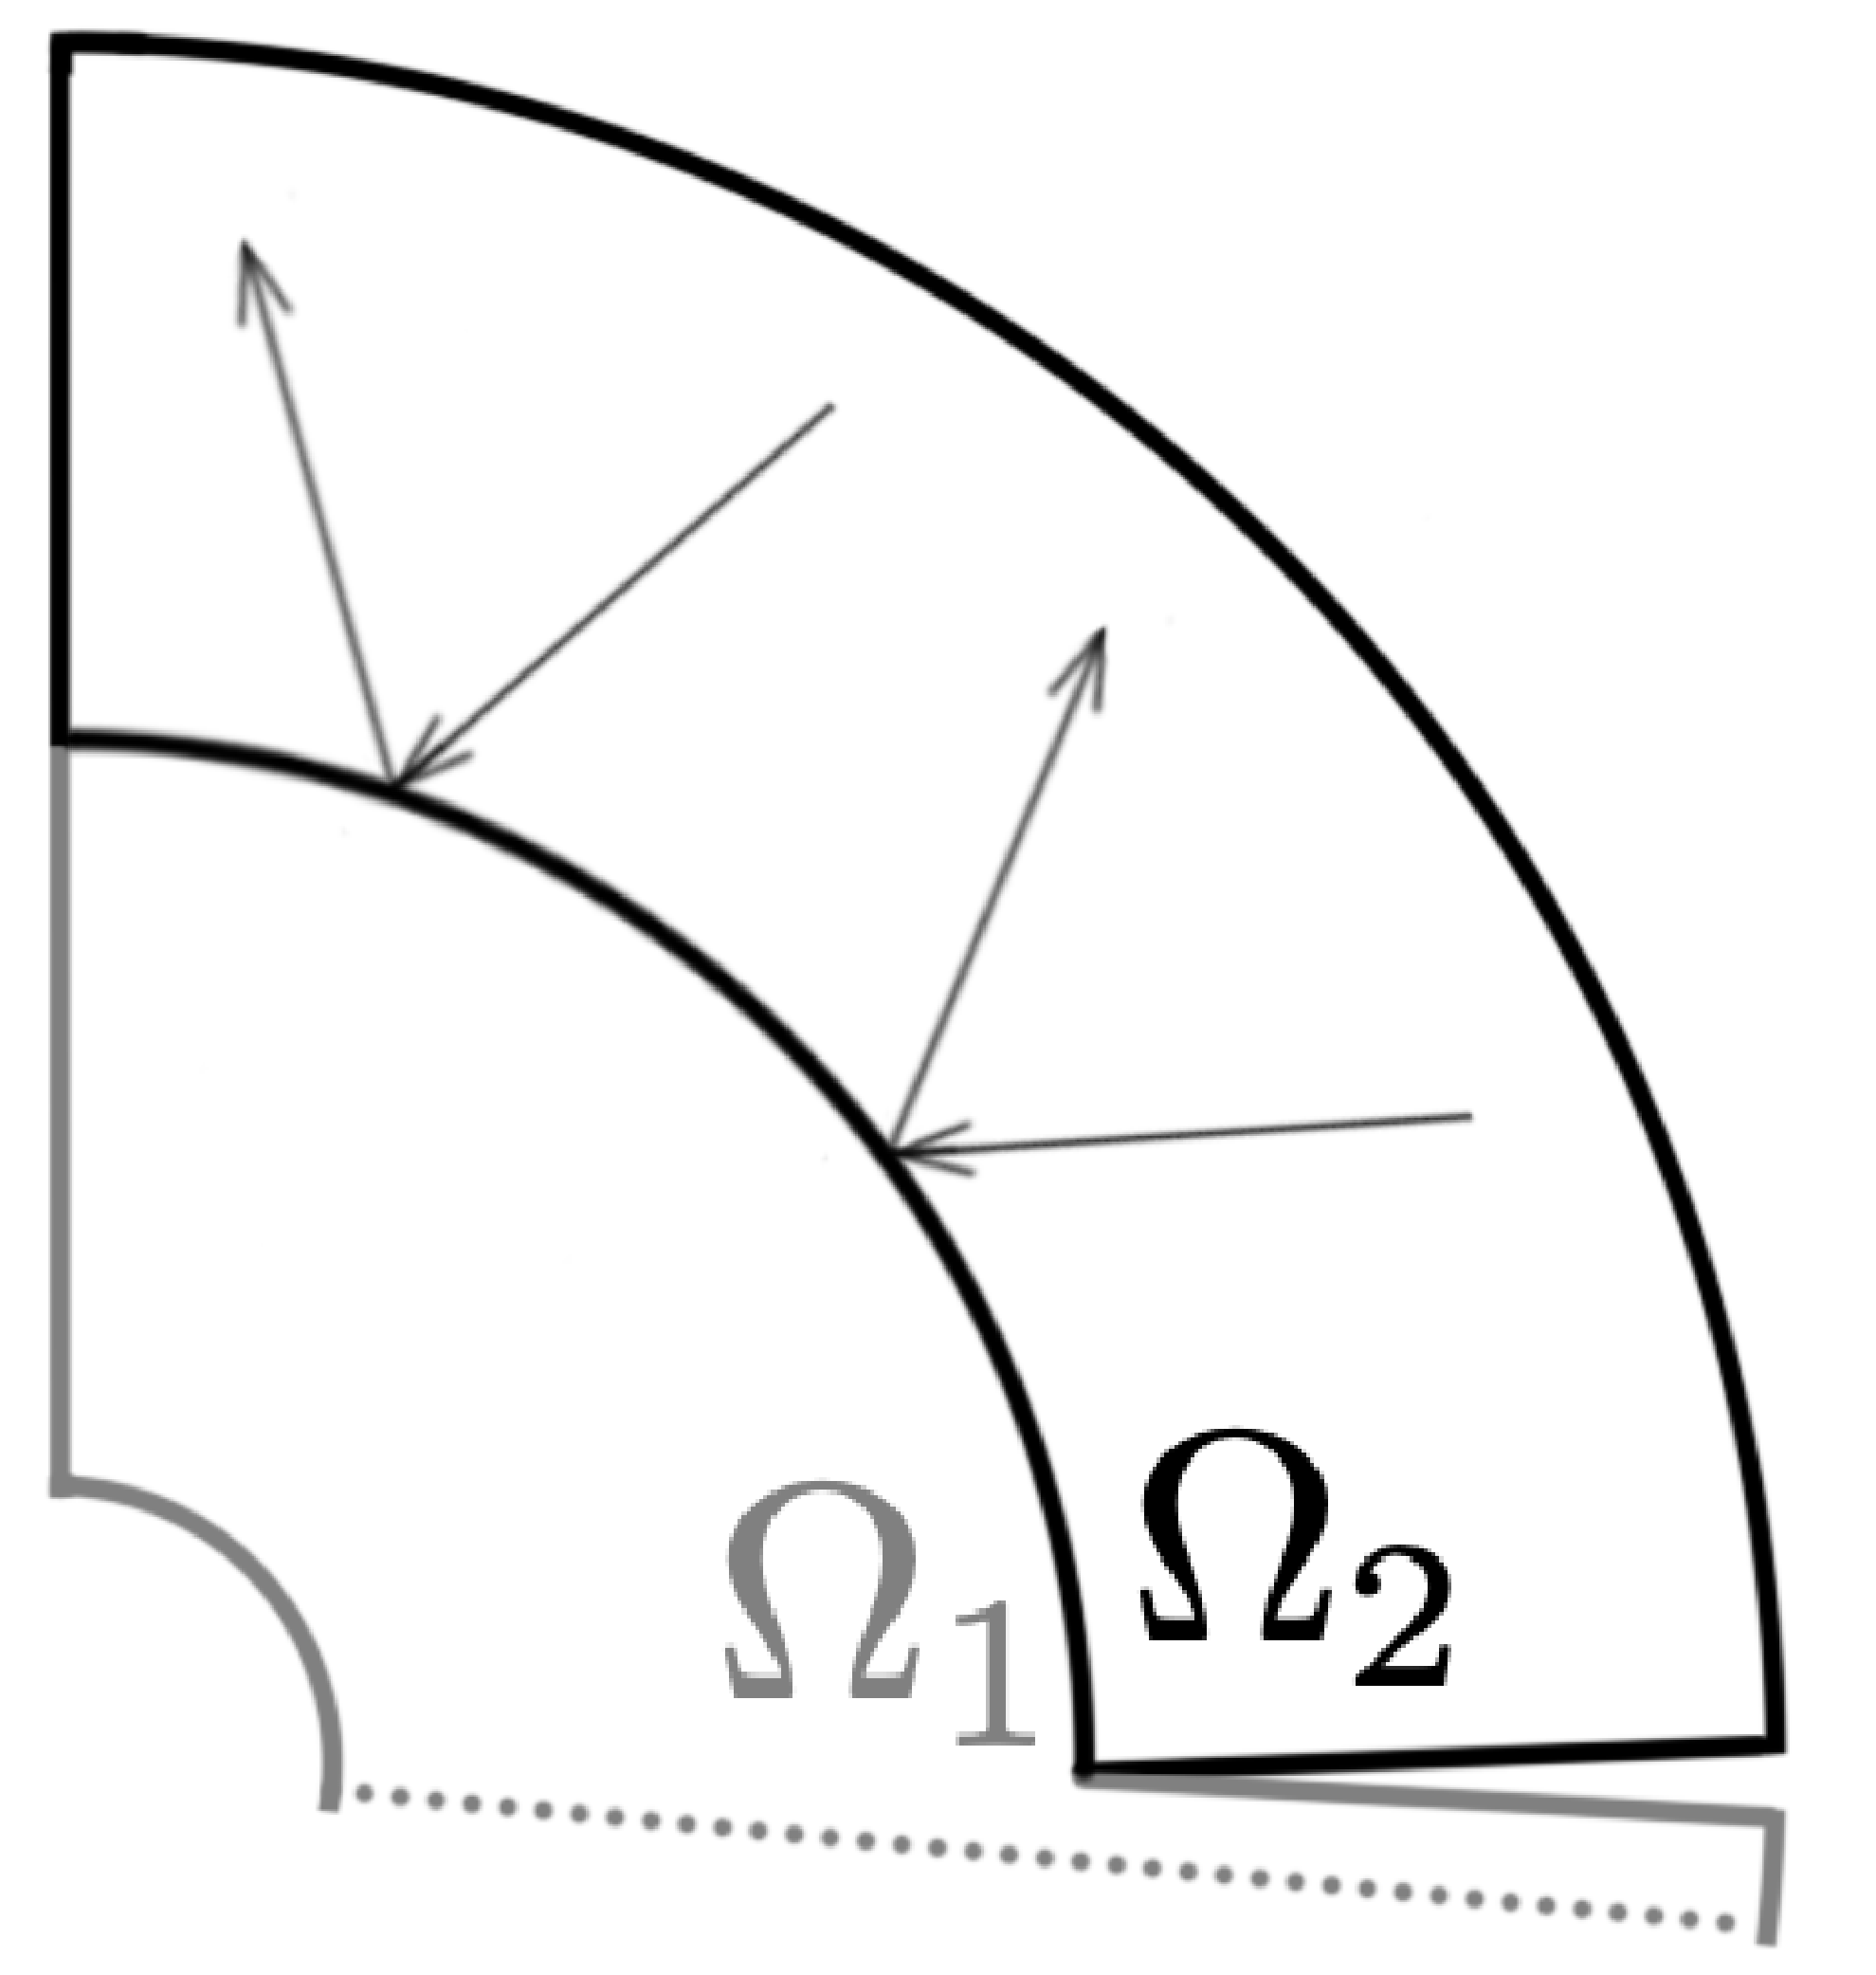
\includegraphics[scale=0.1]{images/ch4/section3_circular/atoms/II/before/before_trajectories.pdf}
    \caption{Пример траекторий до бифуркации, заданных кривыми $II$.}
    \label{fig:pt10:_II_before_trajectories}
\endminipage\hfill
\end{figure}

Для четырех докритических $\widetilde{\Omega}_1, \ldots, \widetilde{\Omega}_4$ сохраним нумерацию по правилу \eqref{eq:foc_numeration_circle}. Добавим к склейке два семиугольника, которые проектируются на область, изображенную на рис. \ref{fig:pt10:_II_trajectories_2}. После их склейки по граничным дугам окружностей получается поверхность с краем, изображенная на рис. \ref{fig:pt10:_II_special_surface_1} --- диск с двумя дырками и выделенными отрезками $\beta_0$ на одной из его граничных окружностей.

\begin{figure}[!htb]
\minipage{0.5\textwidth}
\centering
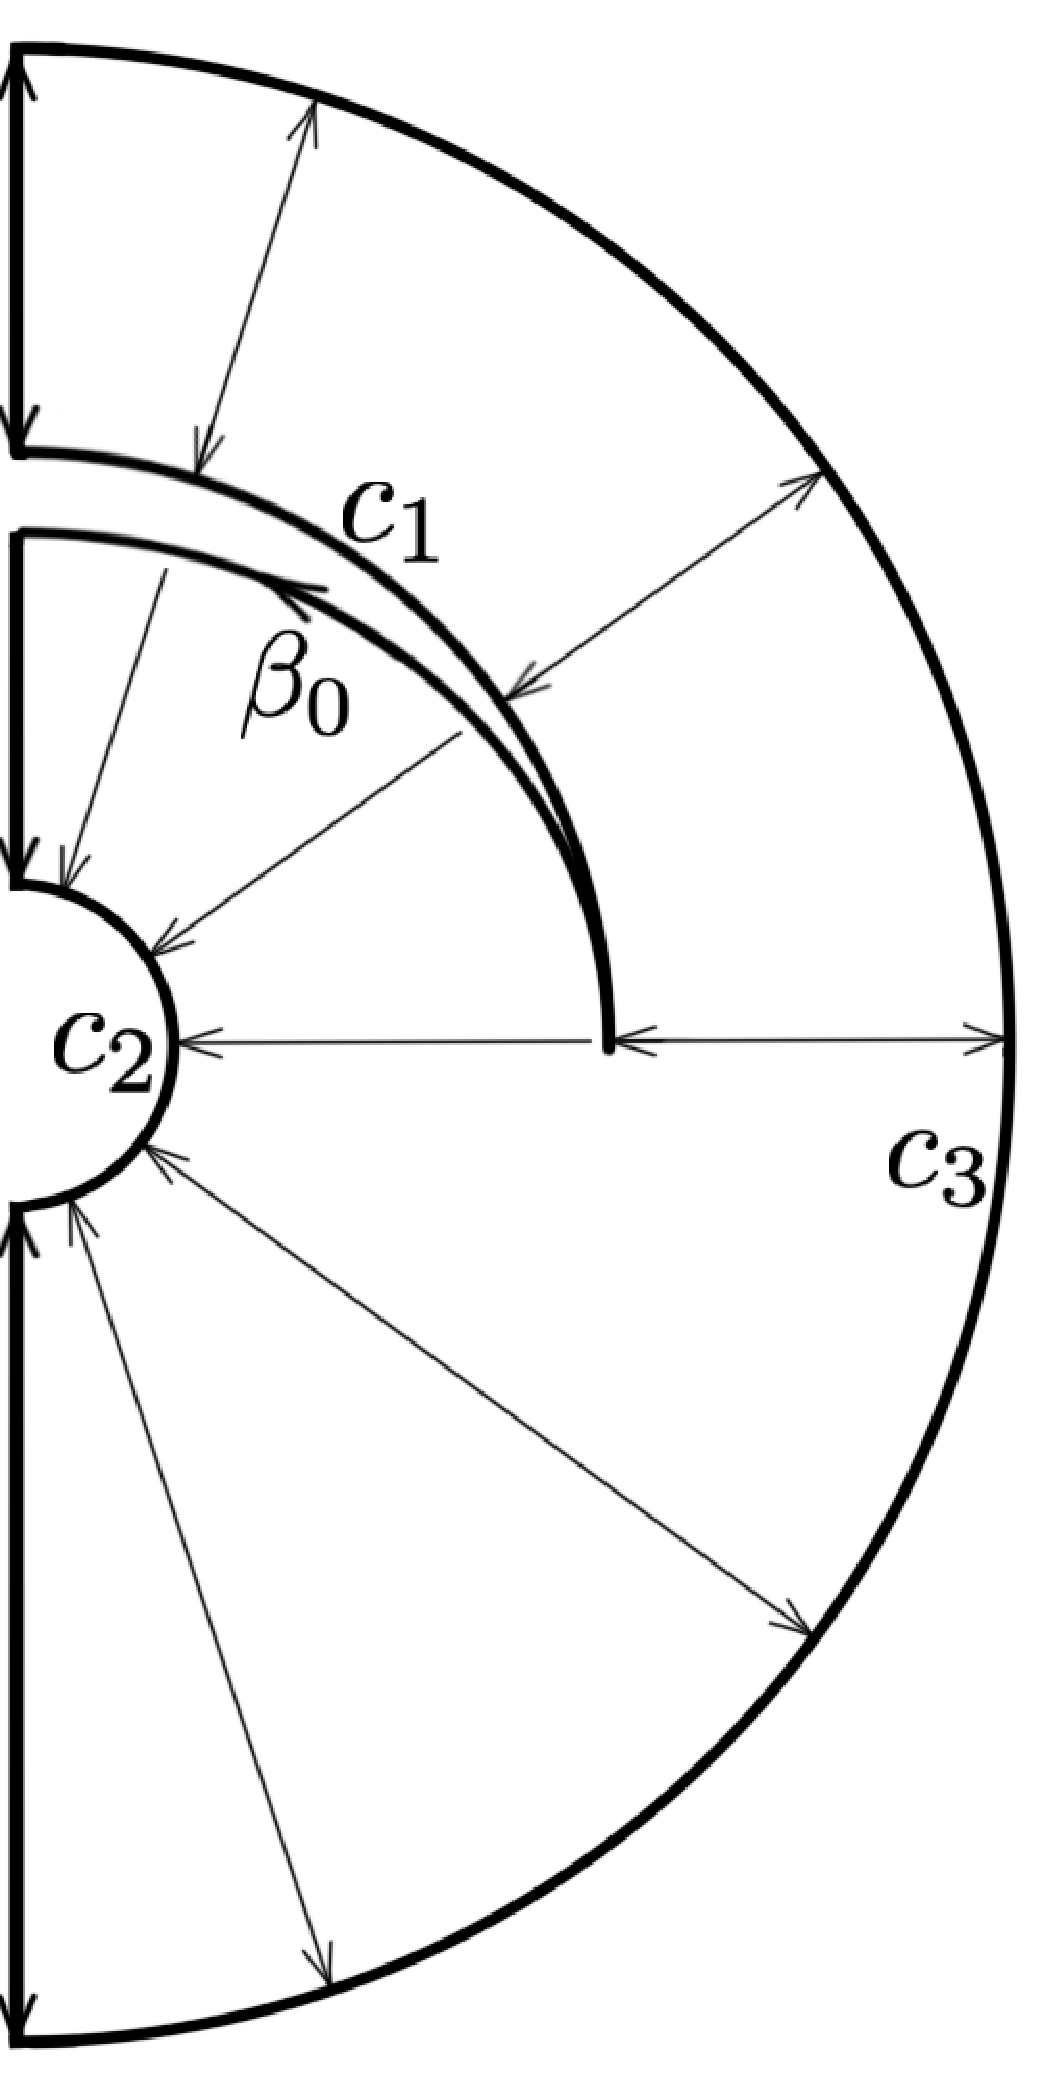
\includegraphics[scale=0.11]{images/ch4/section3_circular/atoms/II/bifurcation/trajectories_2.pdf}
    \caption{Пример траекторий на новом листе.}
        \label{fig:pt10:_II_trajectories_2}
\endminipage\hfill
\minipage{0.5\textwidth}
\centering
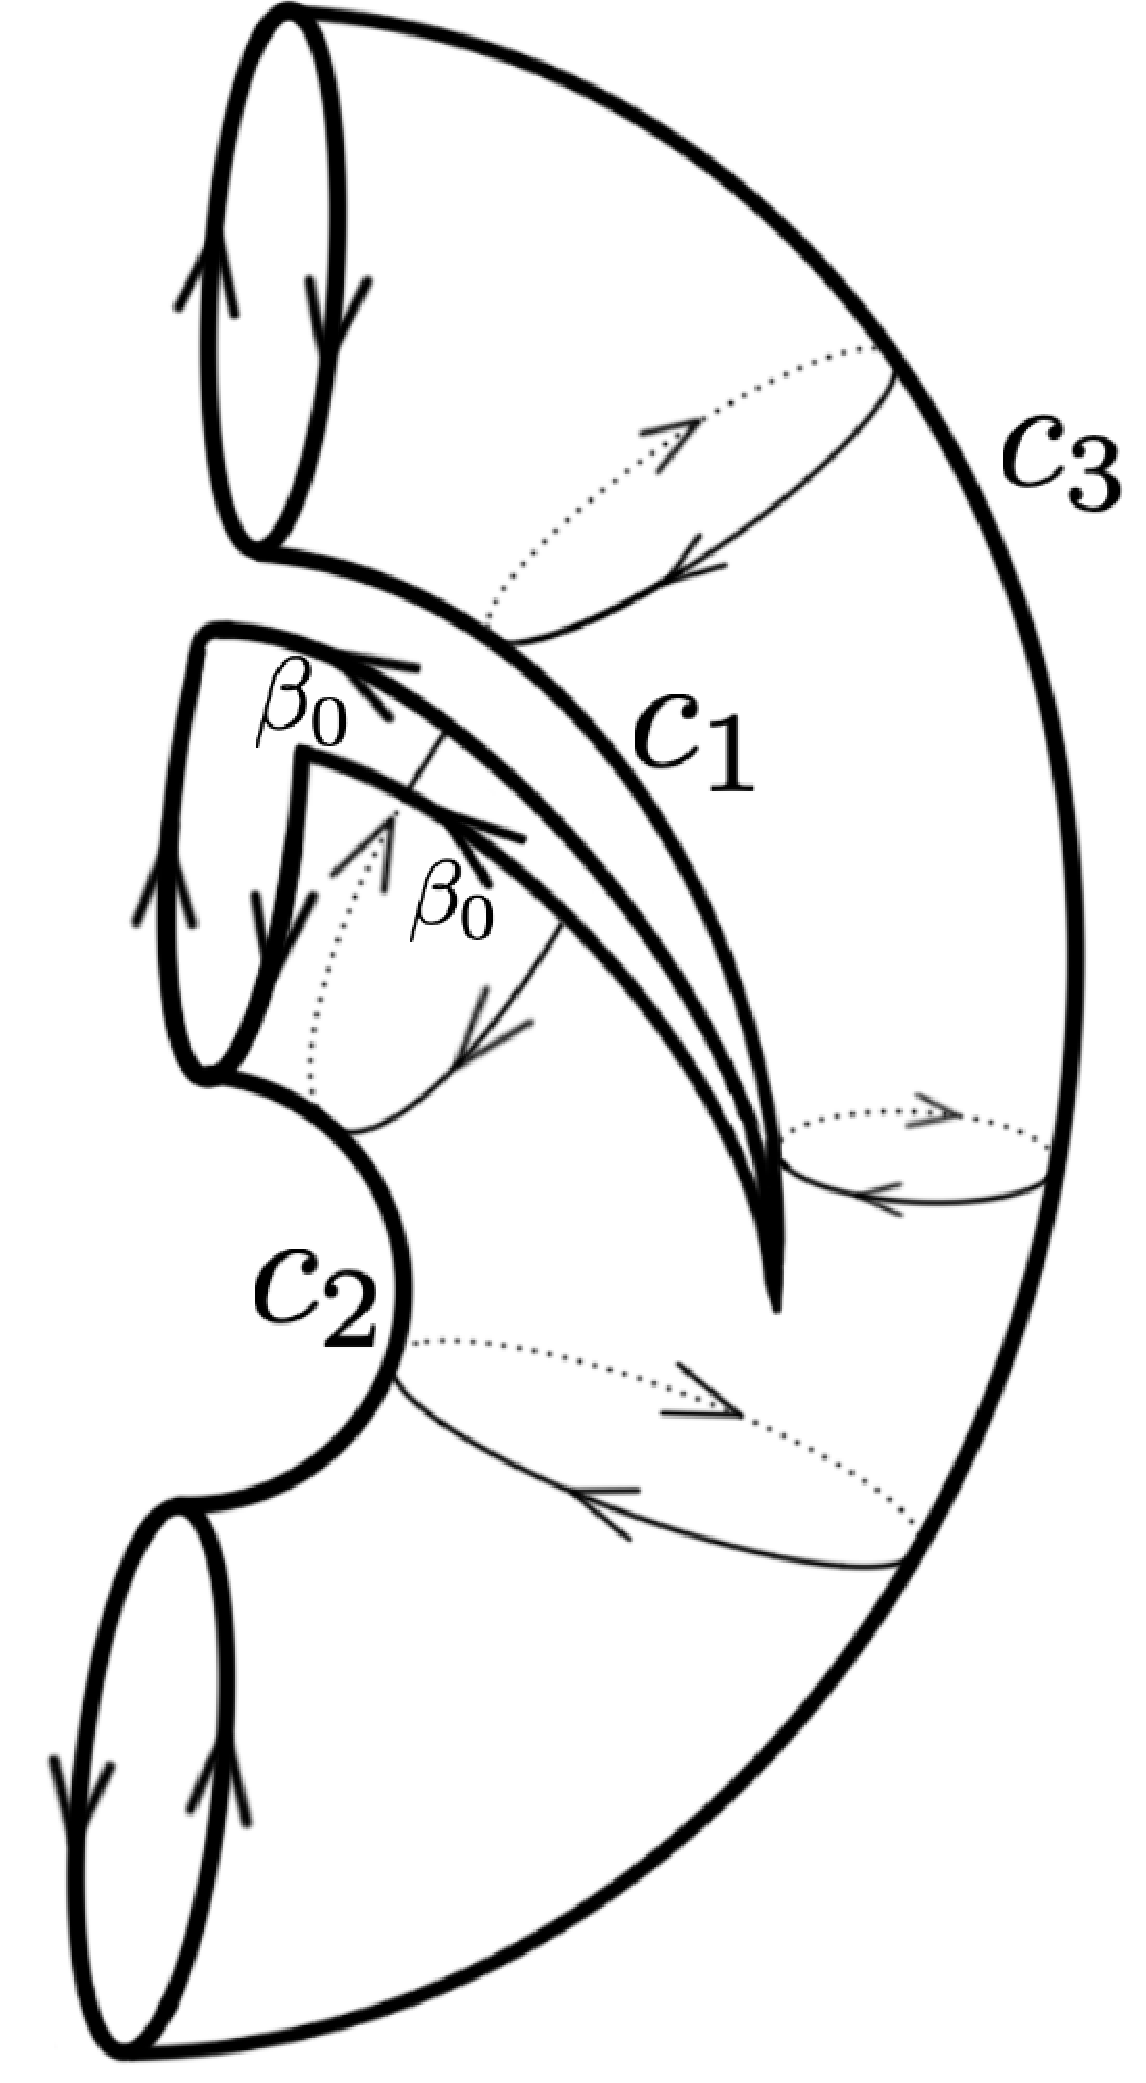
\includegraphics[scale=0.11]{images/ch4/section3_circular/atoms/II/bifurcation/special_surface_1.pdf}
    \caption{Фрагмент поверхности, образованный новым листом.}
        \label{fig:pt10:_II_special_surface_1}
\endminipage\hfill
\end{figure}
 
 При склейке $\widetilde{\Omega}_1$ и $\widetilde{\Omega}_2$ (а также $\widetilde{\Omega}_3$ и $\widetilde{\Omega}_4$),  как и в разделе \ref{sec:ch5/sec6}, нужно отождествить дуги $\beta_0 \subset \widetilde{\Omega}_1$  и $\beta_0 \subset \widetilde{\Omega}_2$ и приклеить их к одной из дуг $\beta_0$ на новой поверхности, изображенной на рис.  \ref{fig:pt10:_II_special_surface_1}.
Ко второй дуге $\beta_0$ поверхности с того же рисунка подклеивается дуга $\beta_0$, полученная отождествлением $\beta_0 \subset \widetilde{\Omega}_3$  и $\beta_0 \subset \widetilde{\Omega}_4$.

После бифуркации этот диск с двумя дырками <<надувается>> и превращается в пару ручек, поскольку теперь в прообразе точки добавленного семиугольника не две вершины, как в момент бифуркации, а четыре (см. рис. \ref{fig:pt10:_II_after_surface_segment}).
\begin{figure}[!htb]
\minipage{0.33\textwidth}
\centering
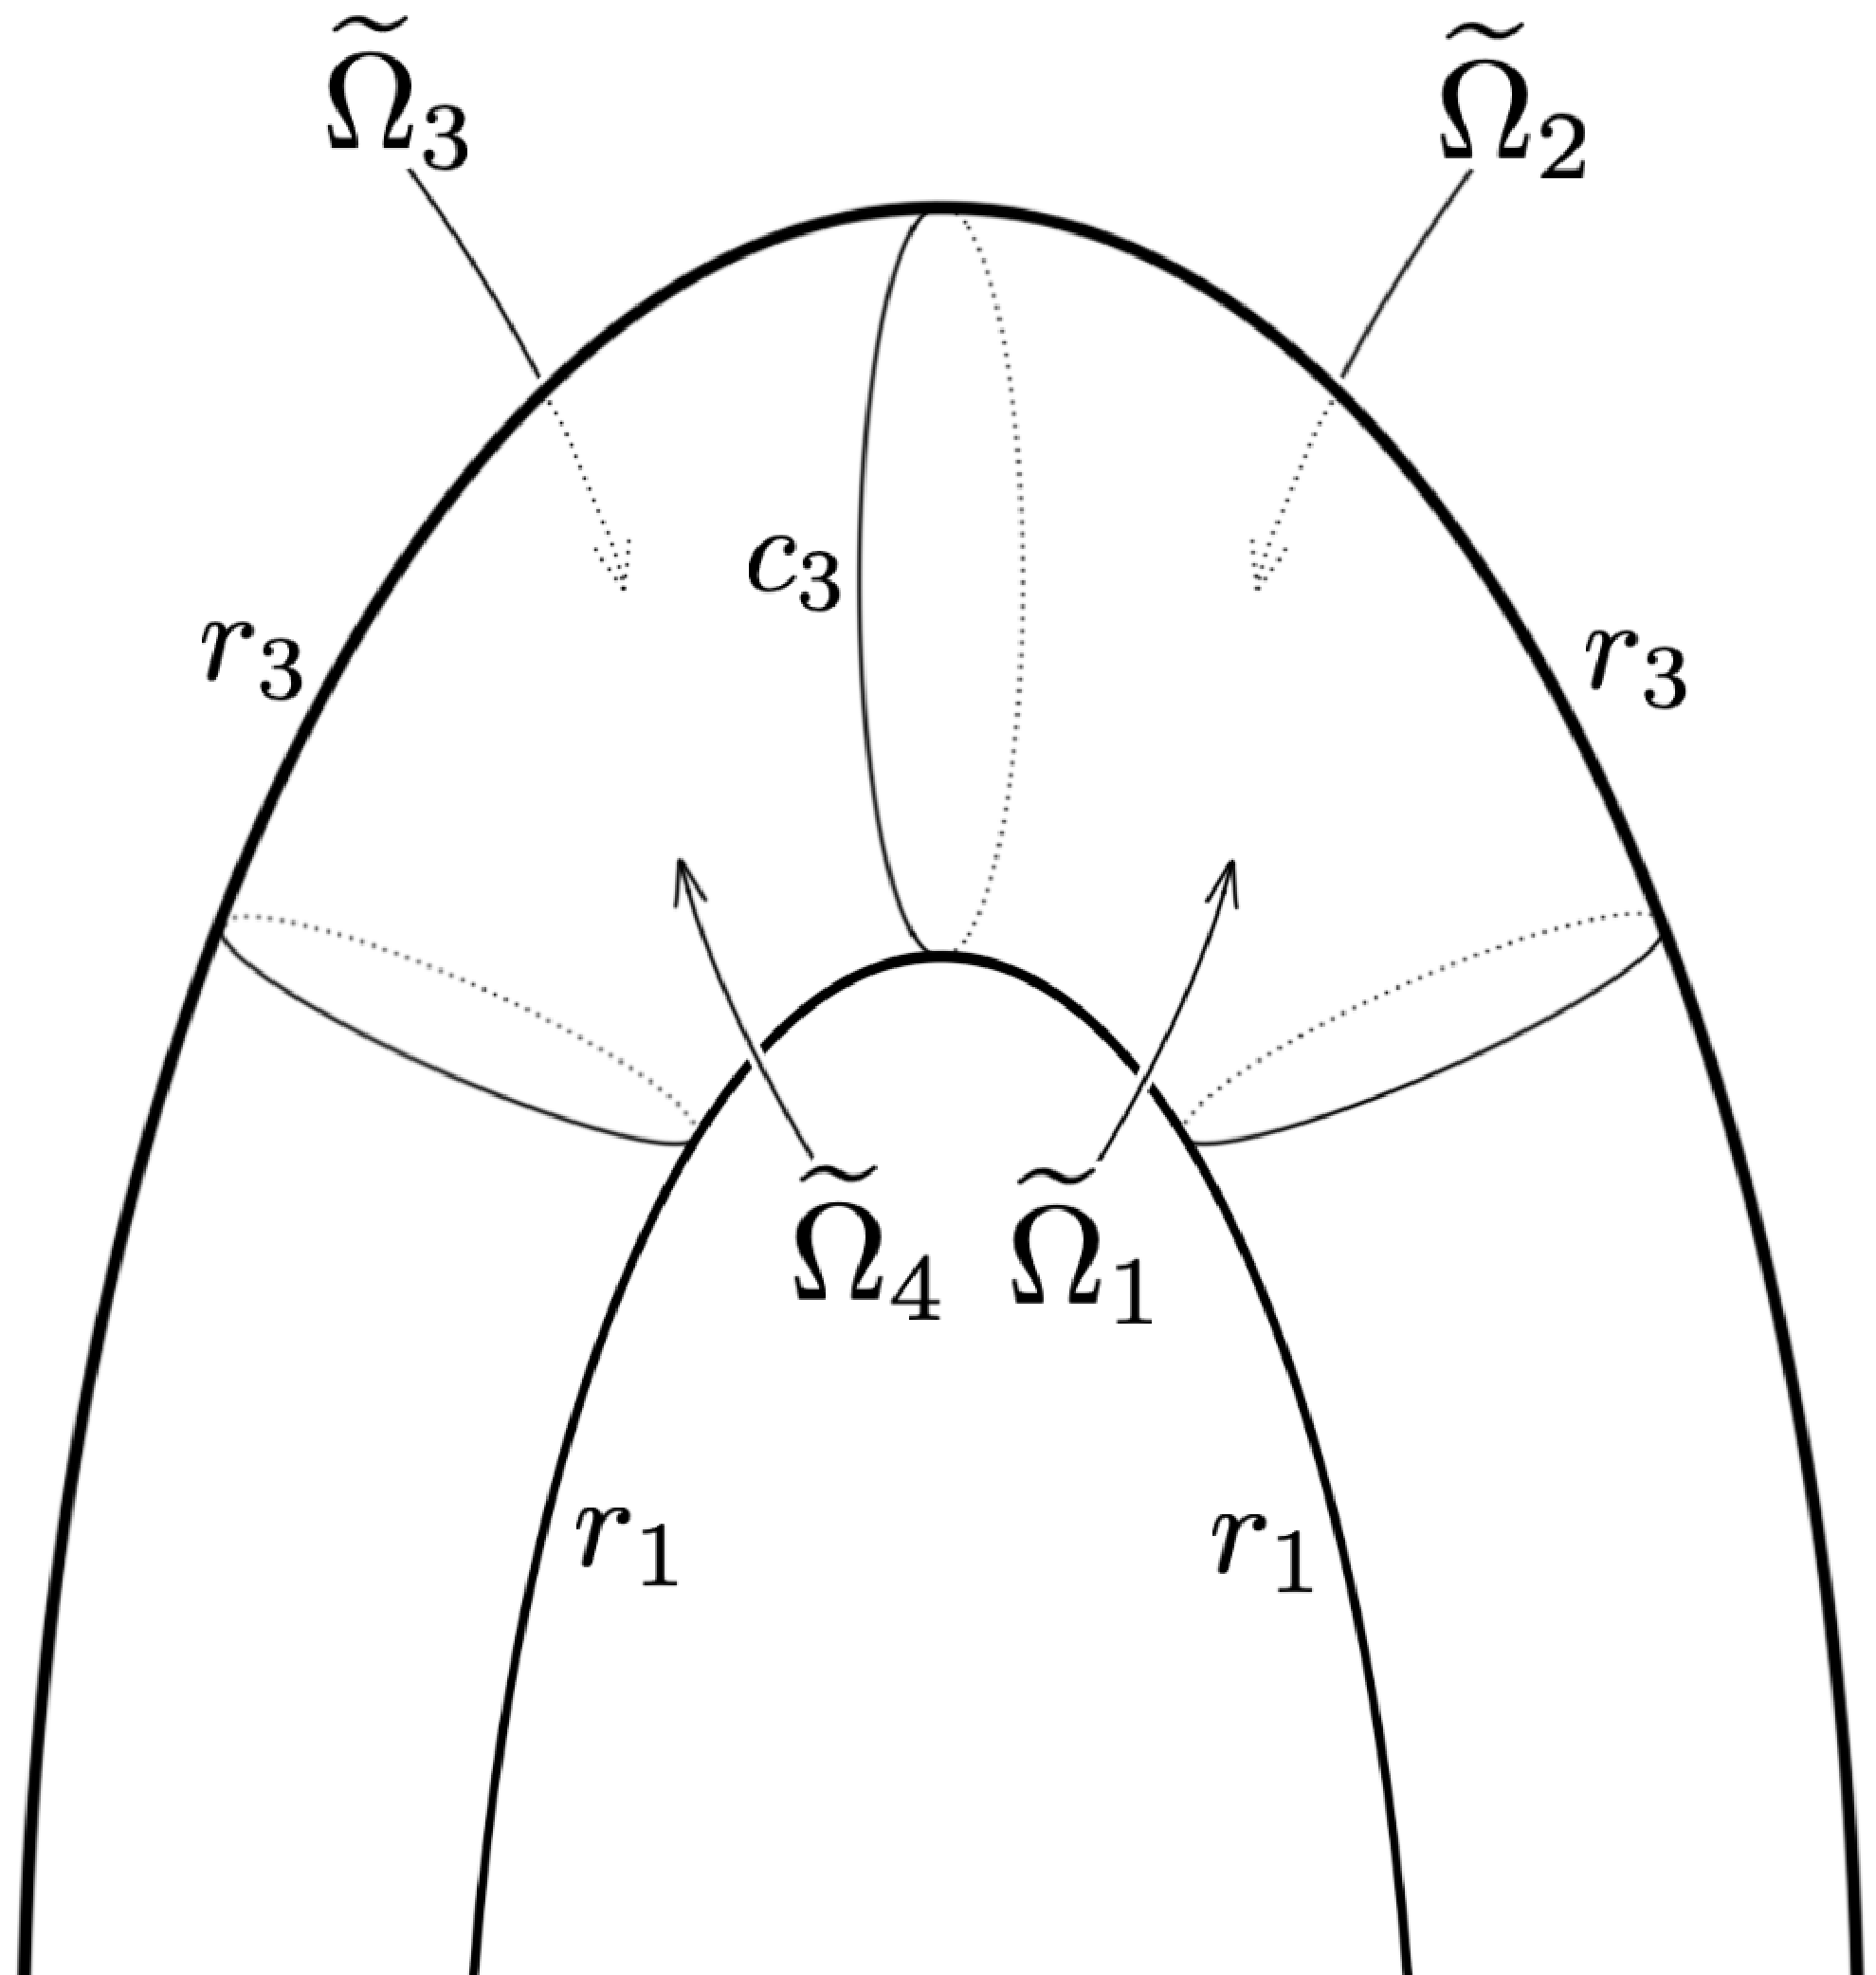
\includegraphics[width=3cm]{images/ch4/section3_circular/atoms/II/before/before_surface_segment.pdf}
    \caption{Фрагмент поверхности до бифуркации.}
        \label{fig:pt10:_II_before_surface}
\endminipage\hfill
\minipage{0.33\textwidth}
\centering
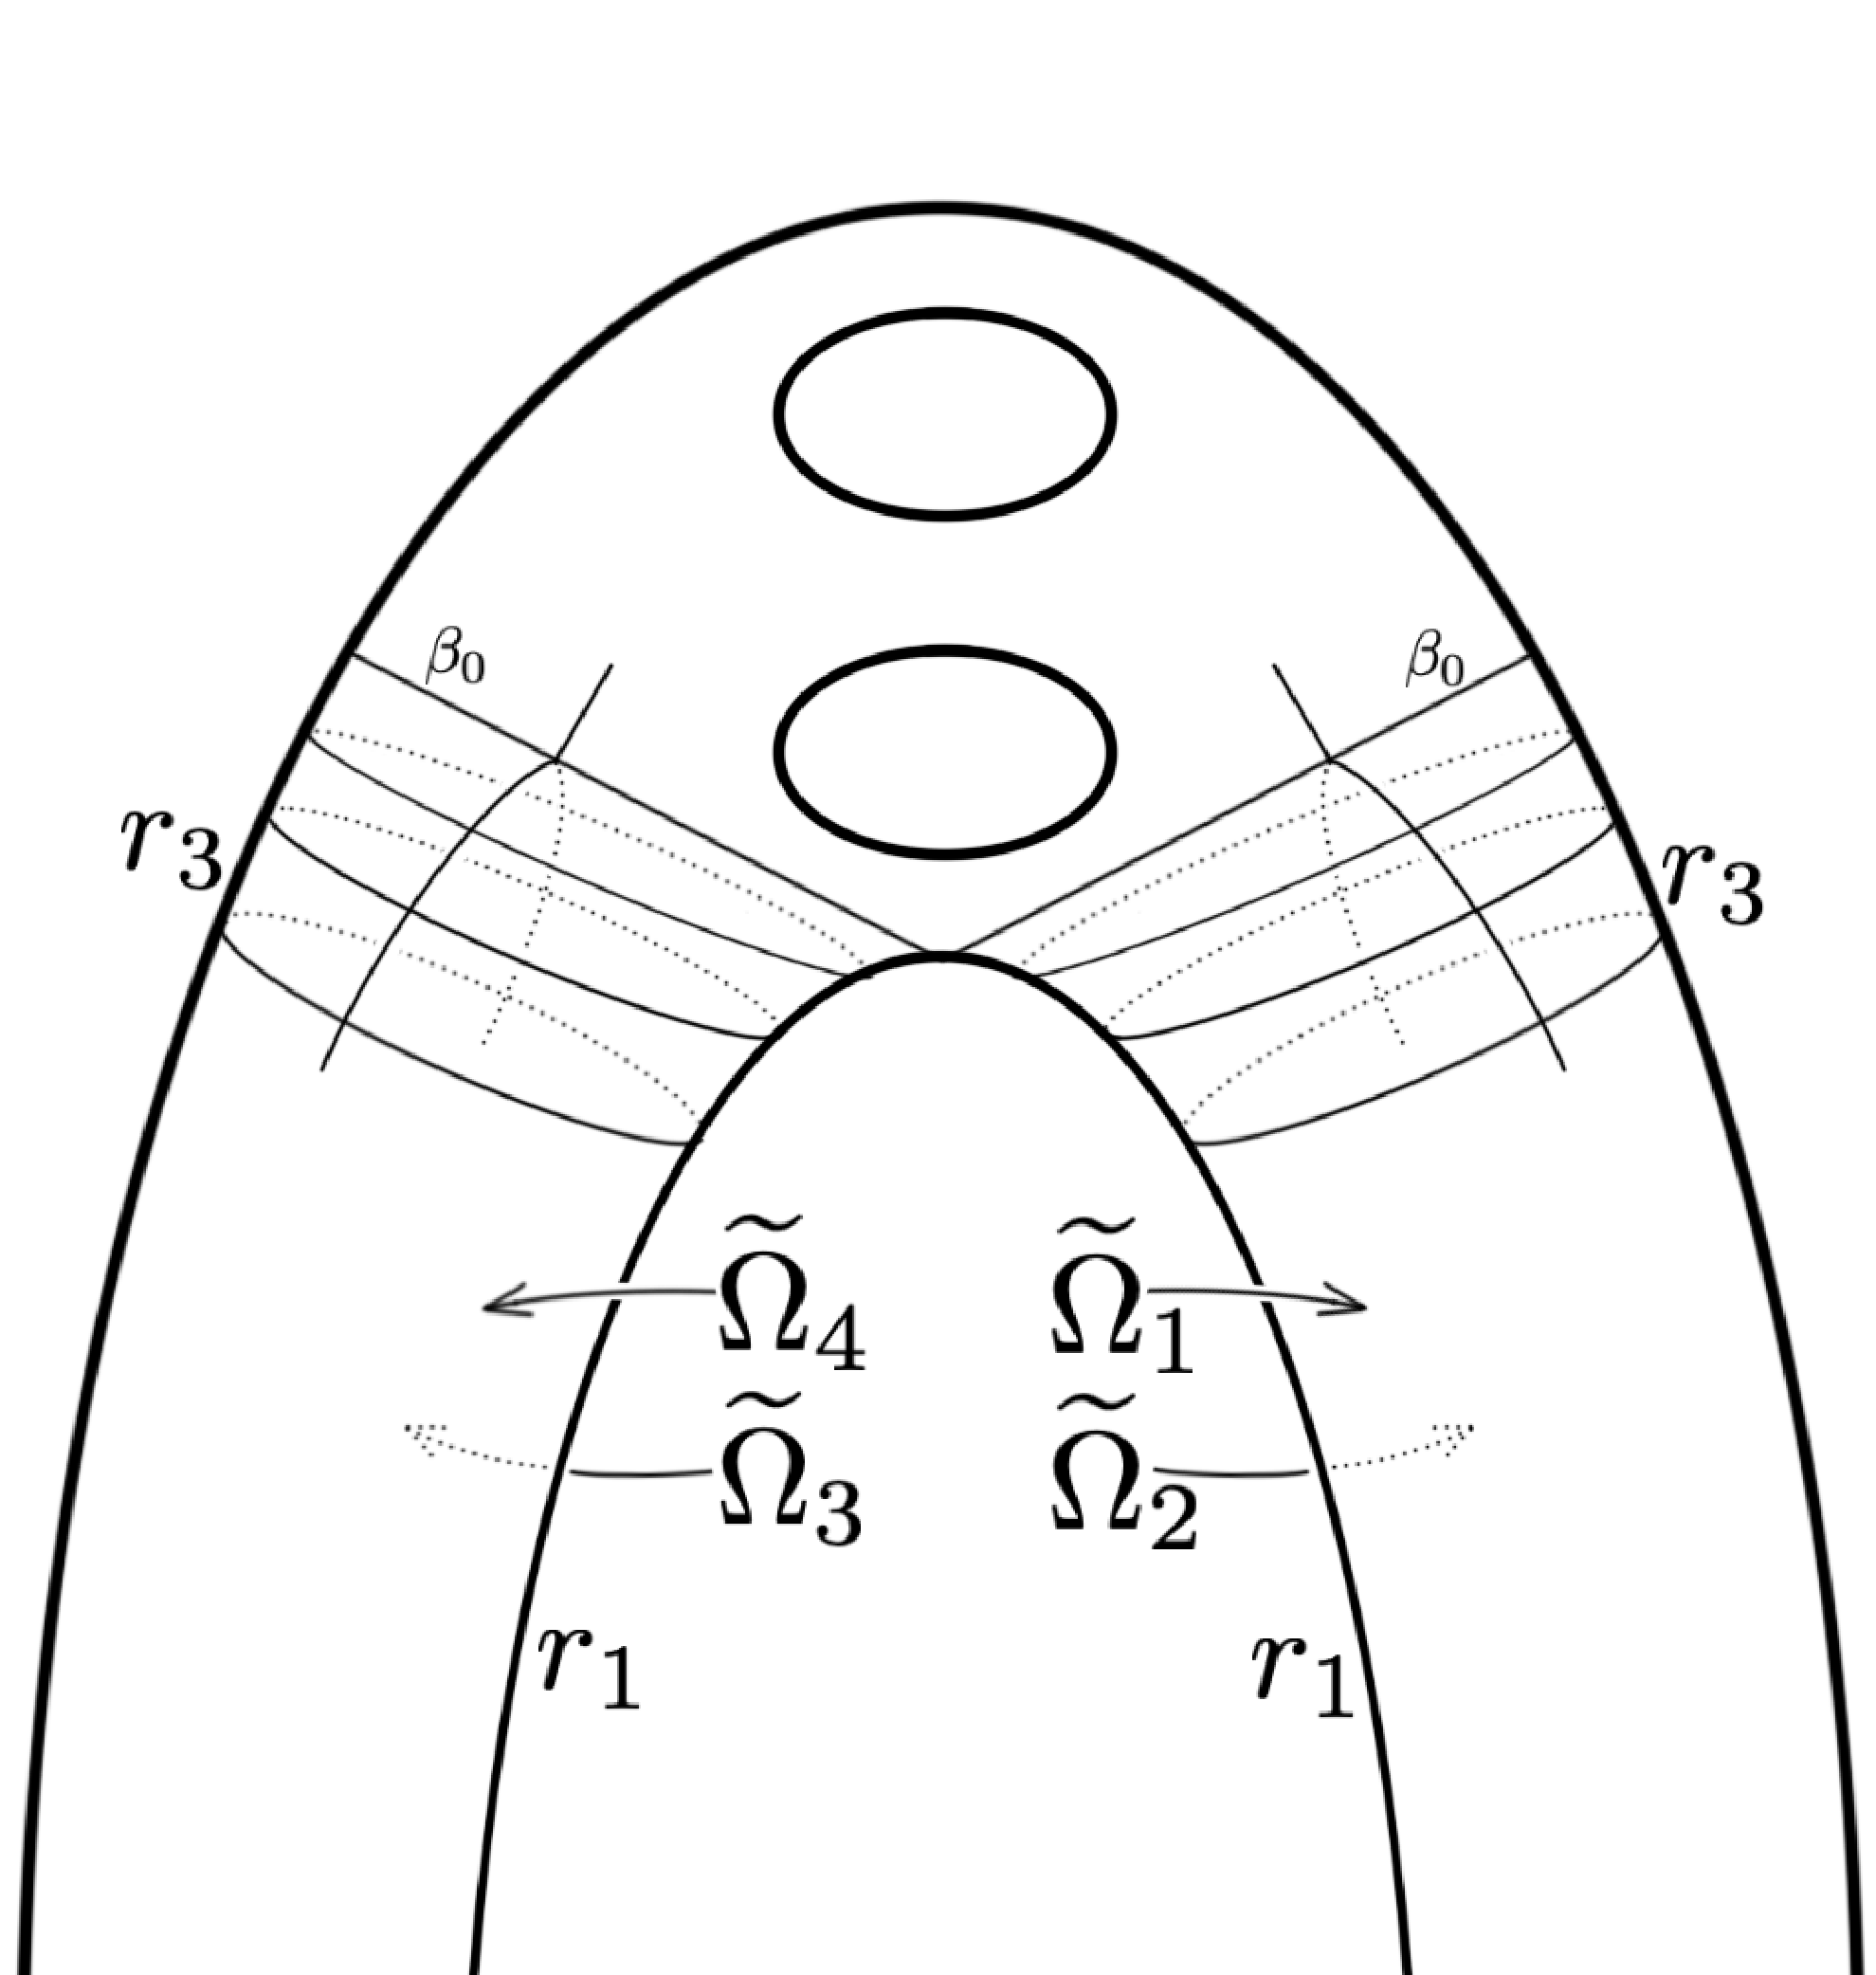
\includegraphics[width=3cm]{images/ch4/section3_circular/atoms/II/bifurcation/surface_segment.pdf}
    \caption{Фрагмент поверхности в момент бифуркации.}
        \label{fig:pt10:_II_surface_segment}
\endminipage\hfill
\minipage{0.33\textwidth}
\centering
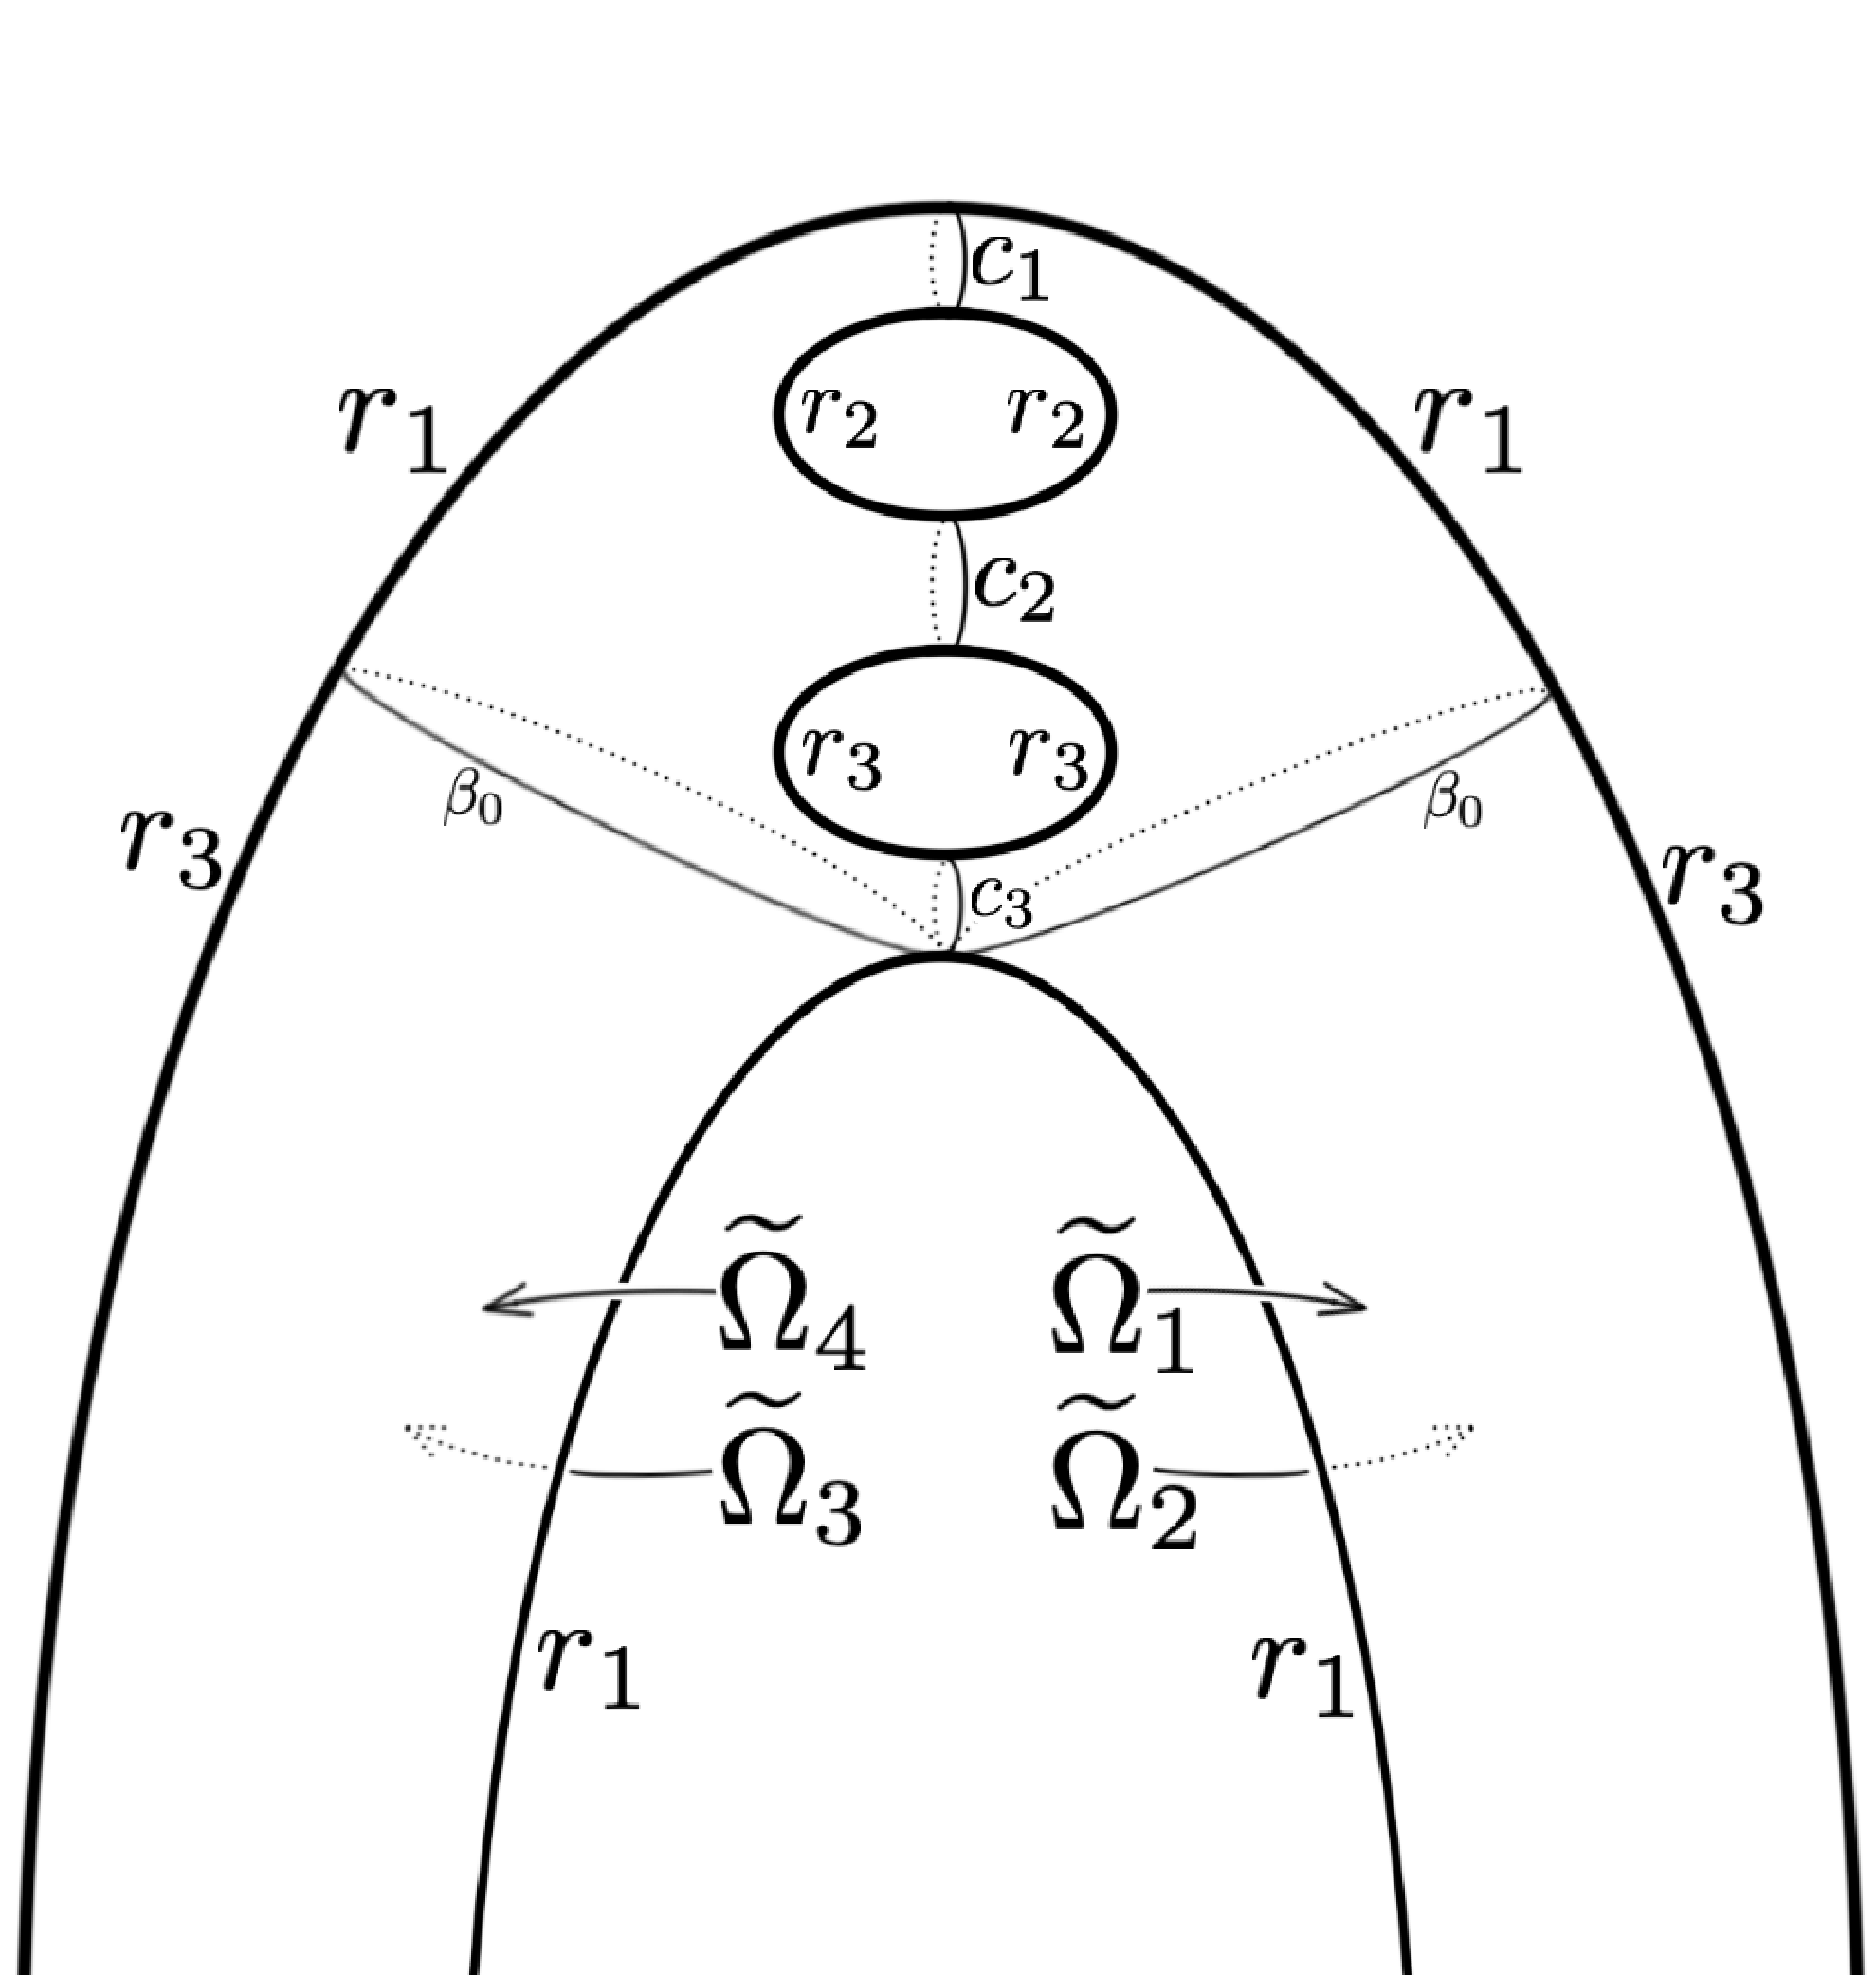
\includegraphics[width=3cm]{images/ch4/section3_circular/atoms/II/after/surface_segment.pdf}
    \caption{Фрагмент поверхности после бифуркации.}
        \label{fig:pt10:_II_after_surface_segment}
\endminipage\hfill
\end{figure}

\subsection{Семейство $III$}
Уравнение произвольной кривой $III_m$ имеет вид 
$$\xi = m \gamma + \varepsilon = ||L_1|| + \left(m - \left\lfloor \frac{||L_1||}{\gamma} \right\rfloor \right) \gamma.$$
Тогда можно выделить особый сегмент большого листа \ref{fig:pt10:_big_domain_transformed}, соответствующий значению $\xi=||L_1||$, на котором $\rho_1^2 > r_1^2, \ \rho_2^2 = r_1^2$.
Для конкретности считаем, что $\rho_1^2 < r_2^2$.
Получается, что изображенный на рис. \ref{fig:pt10:_III_page_segment_1} шестиугольник в процессе бифуркации <<отрезается>> вдоль дуги, обозначенной $\beta_{k-1}$ на листе $\widetilde{\Omega}$ (см. рис. \ref{fig:pt10:_big_domain_transformed}). 
Рассмотрим эту часть листа $\widetilde{\Omega}$.
\begin{figure}[!htb]
\minipage{0.5\textwidth}
\centering
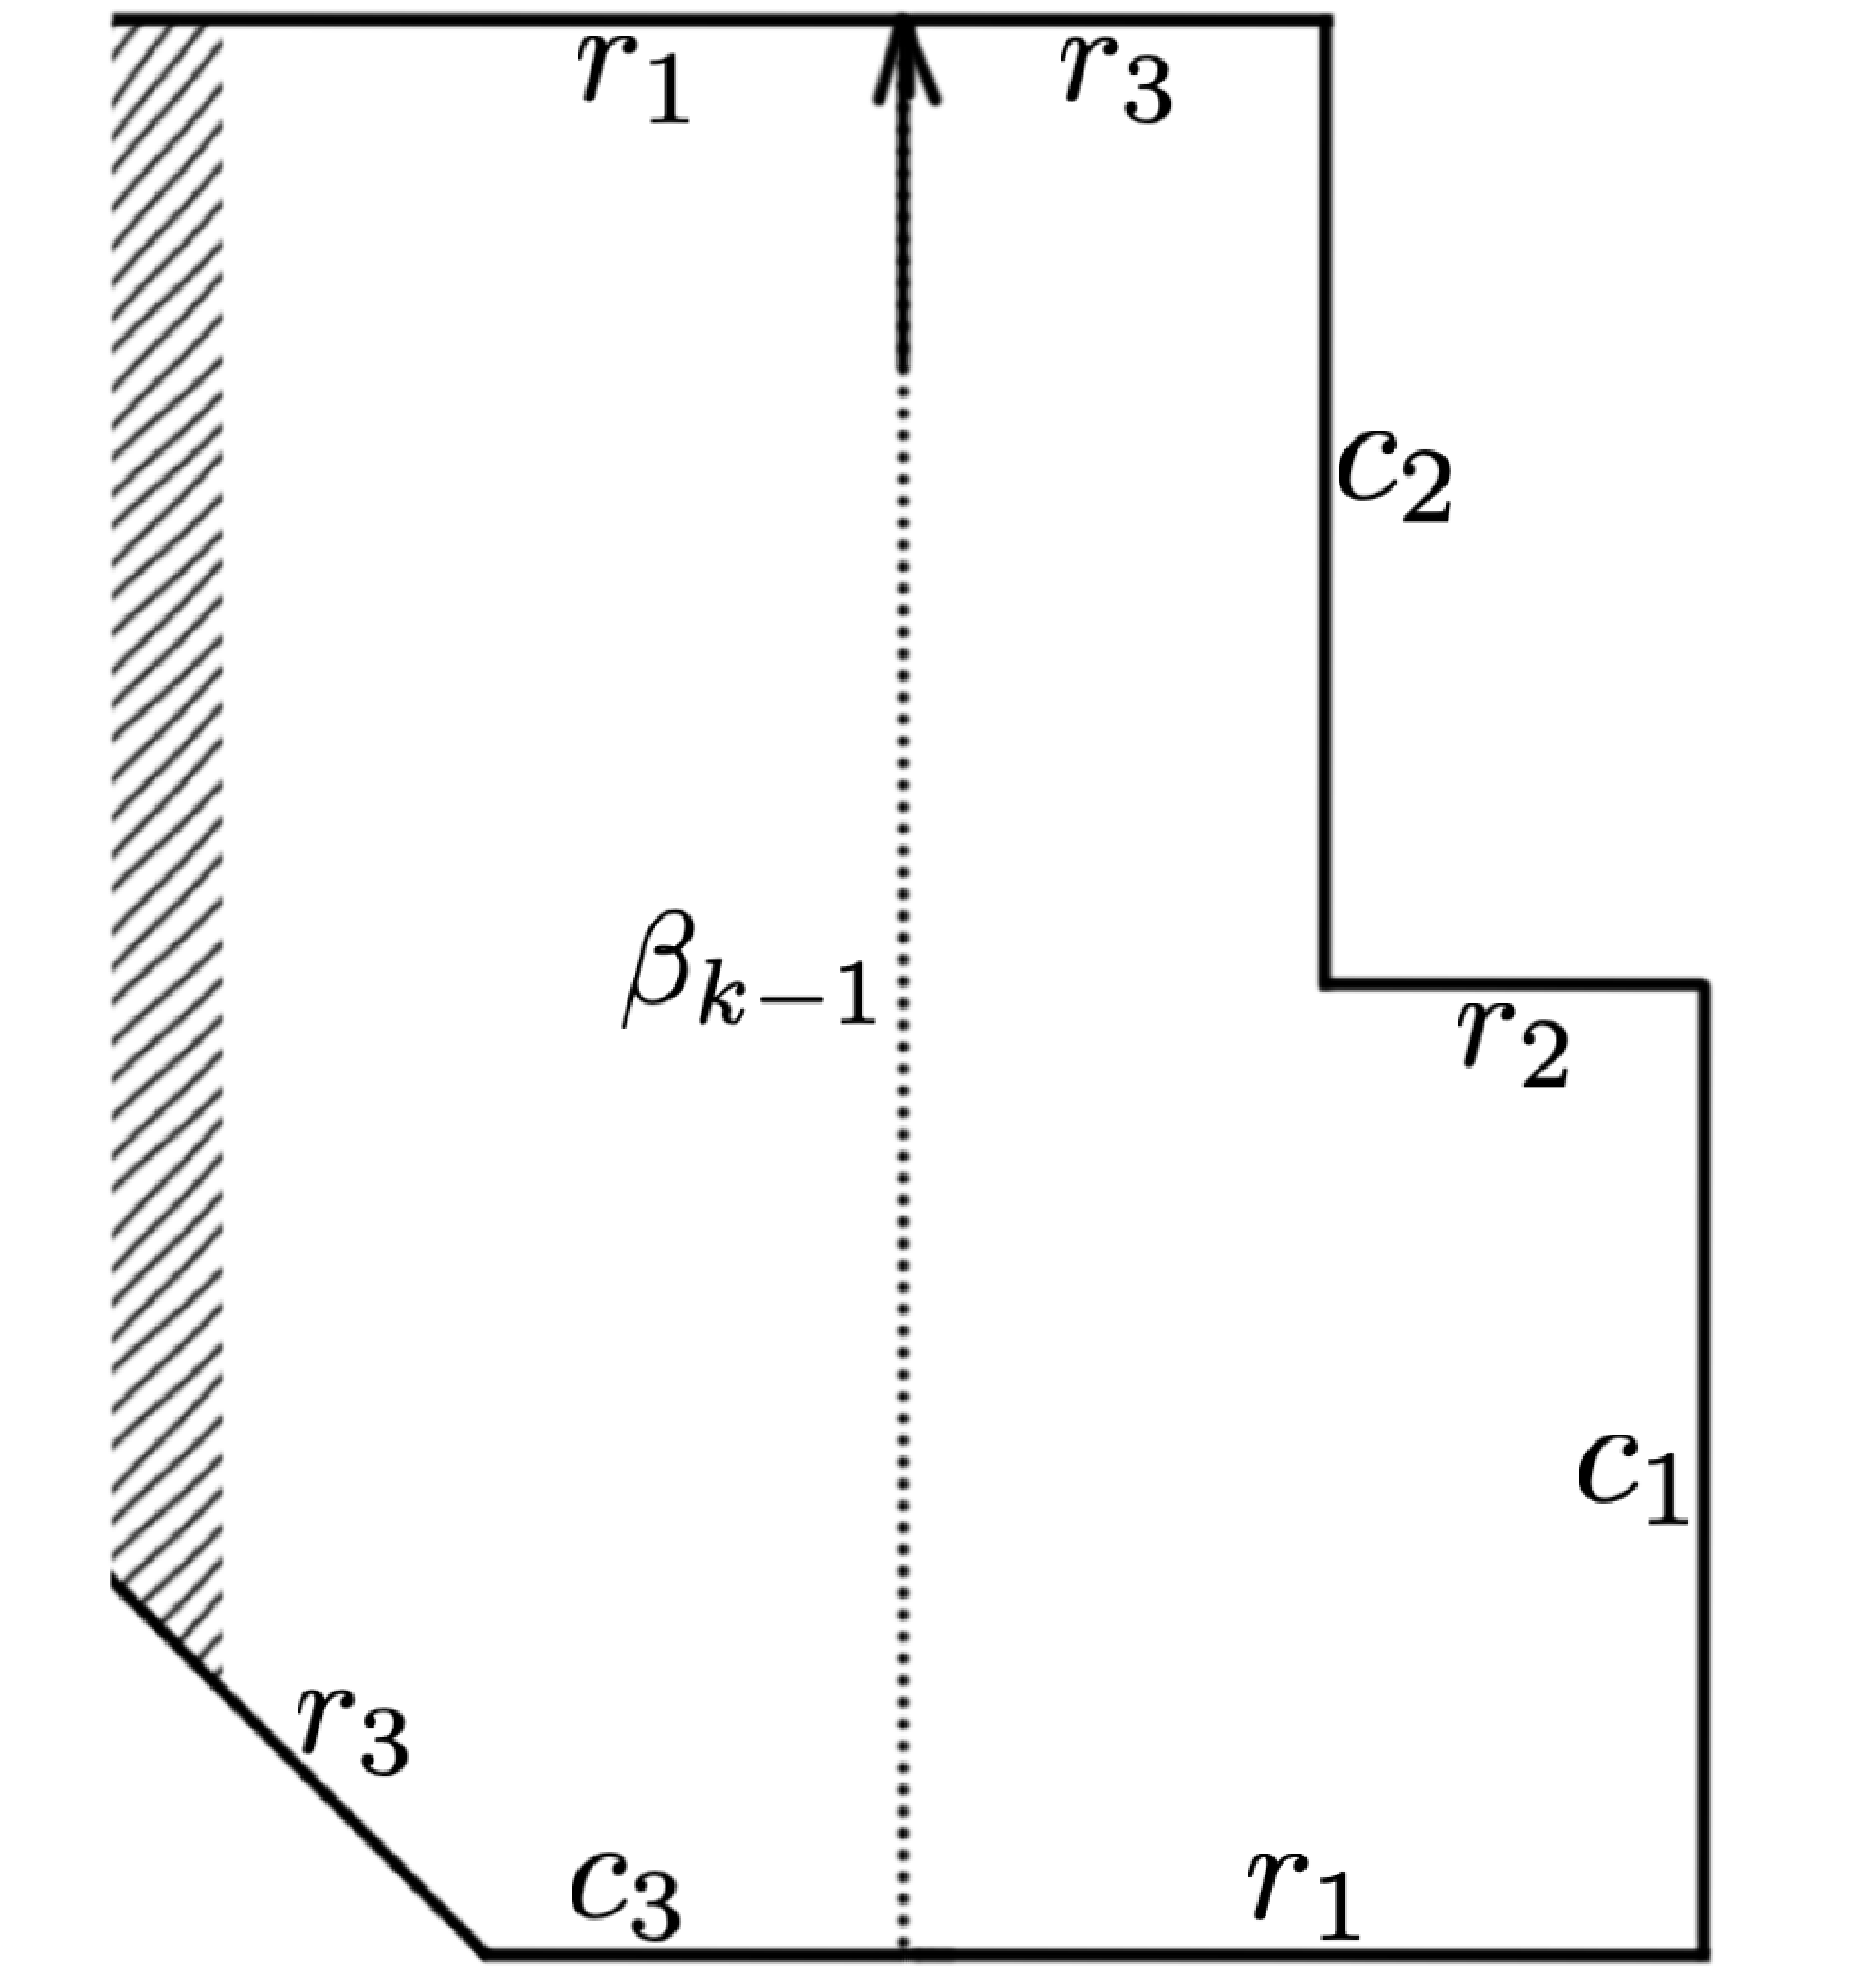
\includegraphics[scale=0.11]{images/ch4/section3_circular/atoms/III/page_segment_1.pdf}
    \caption{Лист $\widetilde{\Omega}$ до бифуркации.}
    \label{fig:pt10:_III_page_segment_1}
\endminipage\hfill
\minipage{0.5\textwidth}
\centering
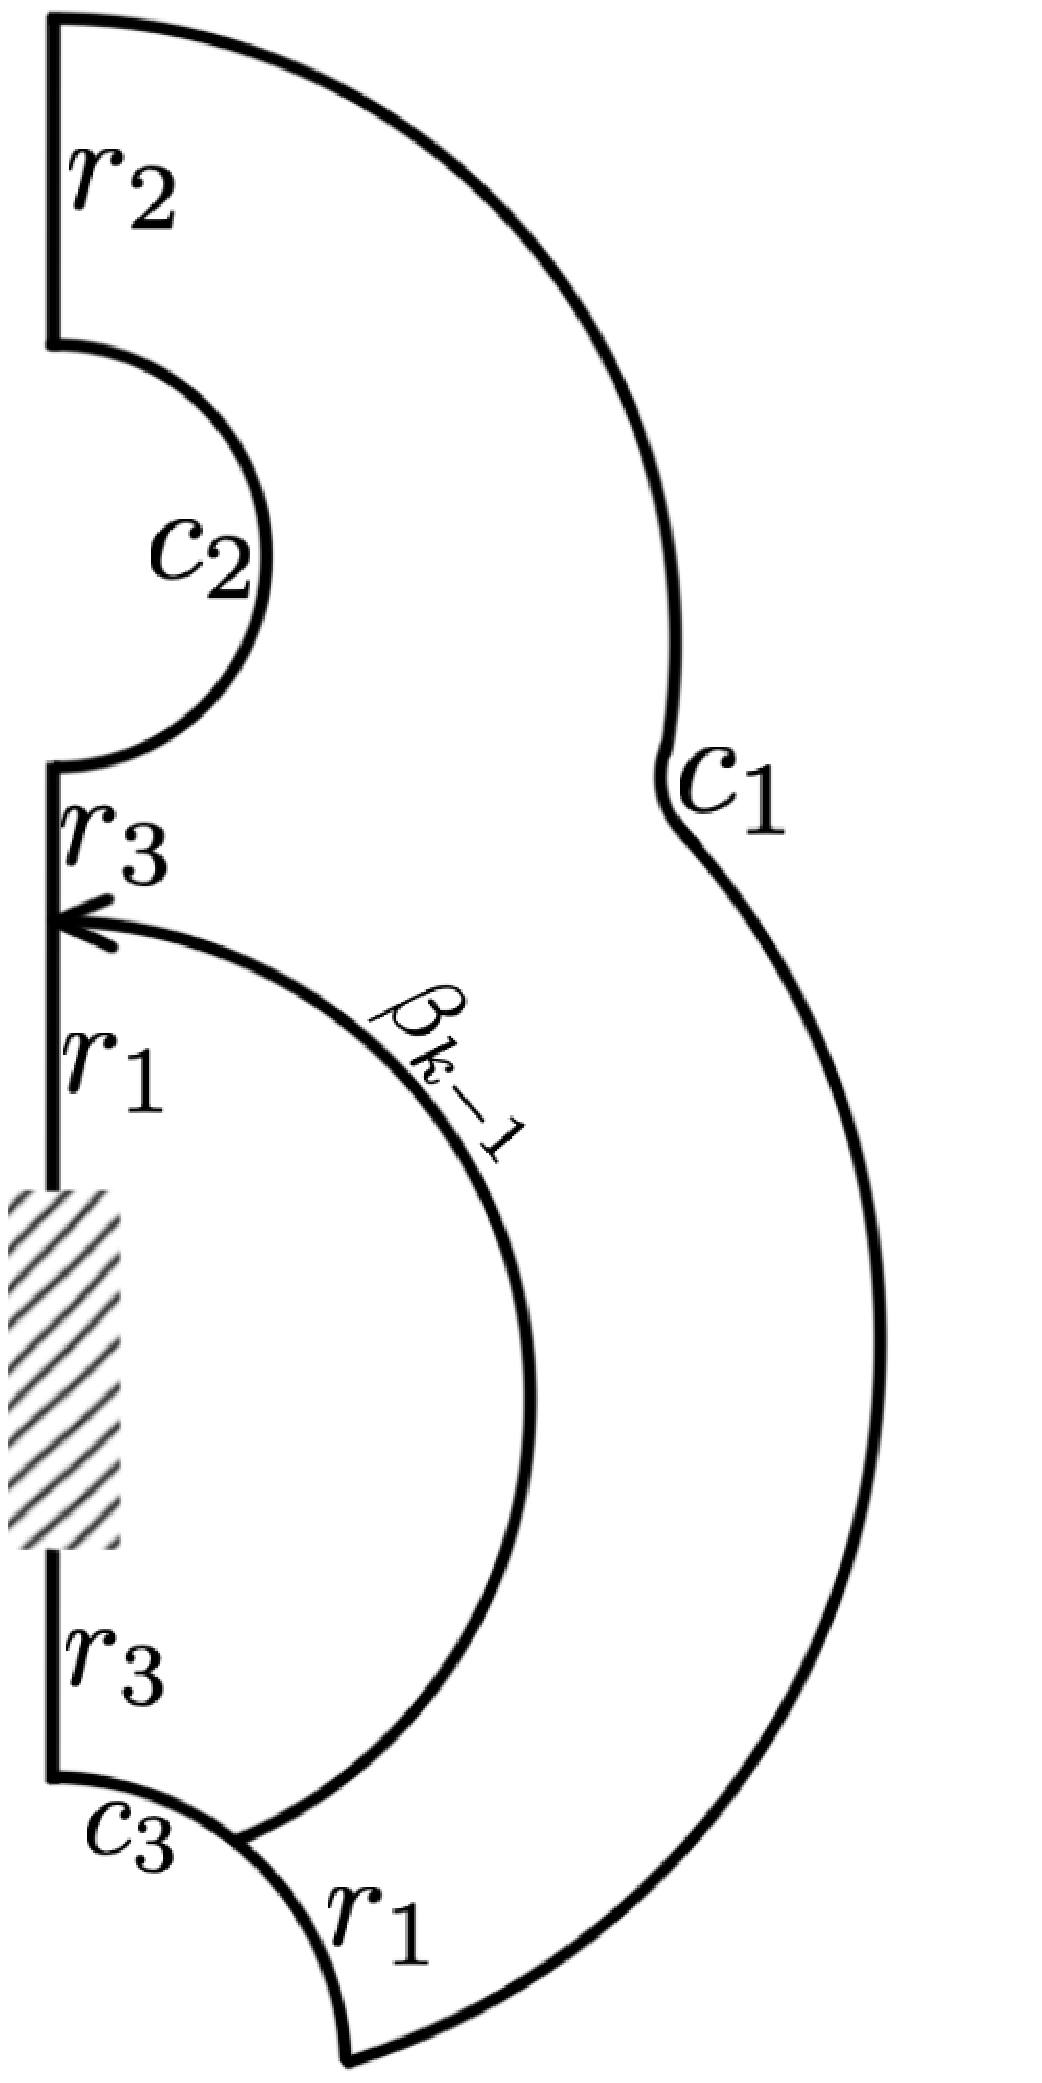
\includegraphics[scale=0.12]{images/ch4/section3_circular/atoms/III/page_segment_2.pdf}
    \caption{Лист $\widetilde{\Omega}$ до бифуркации.}
        \label{fig:pt10:_III_page_segment_2}
\endminipage\hfill
\end{figure}

Заштрихованная часть листа не изменится, если мы пересекаем только одну прямую. Преобразуем лист склейки, чтобы результат выглядел как на рис. \ref{fig:pt10:_III_page_segment_2}.

\begin{figure}[!htb]
\minipage{0.5\textwidth}
\centering
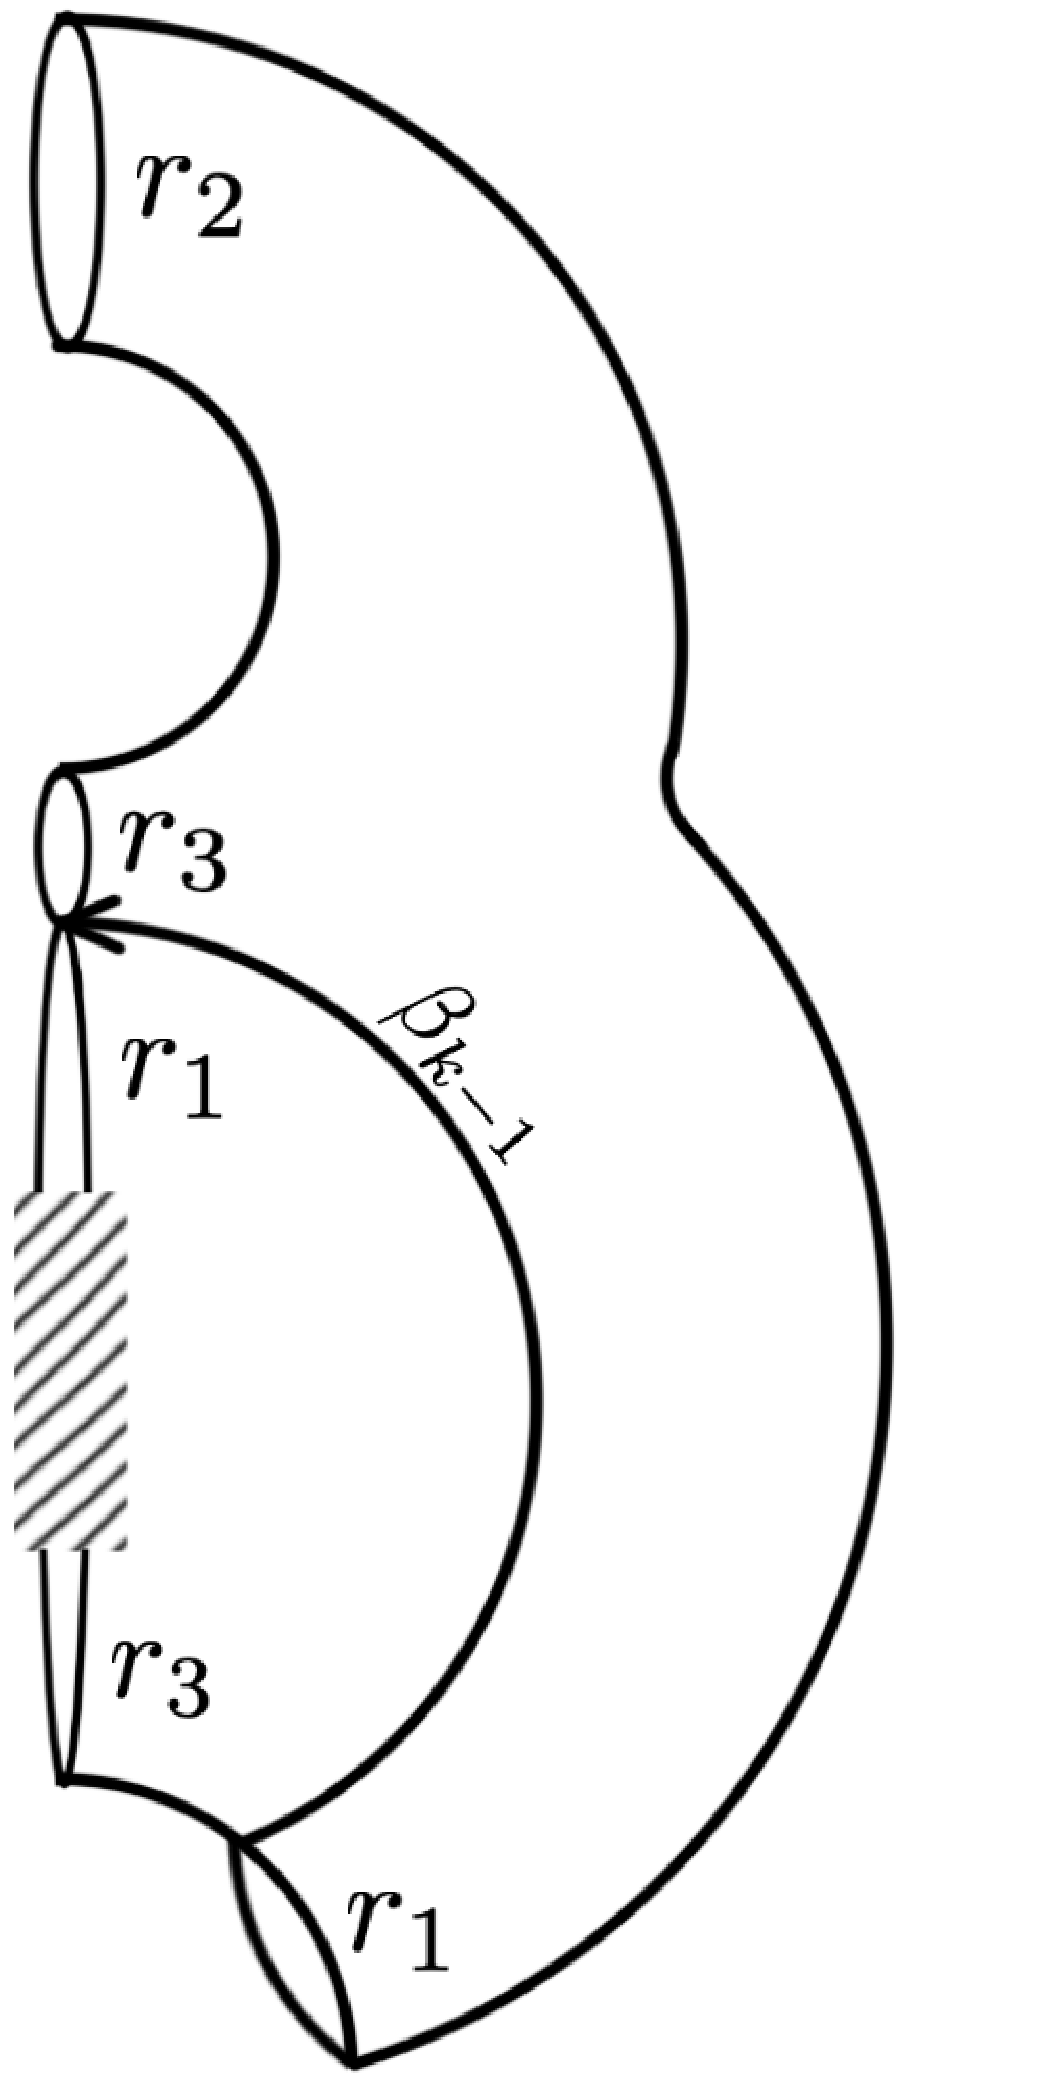
\includegraphics[scale=0.11]{images/ch4/section3_circular/atoms/III/surface_half.pdf}
    \caption{Склейка $\Omega_1 \cup \Omega_4$ по правилу склейки $c$.}
    \label{fig:pt10:_III_surface_half}
\endminipage\hfill
\minipage{0.5\textwidth}
\centering
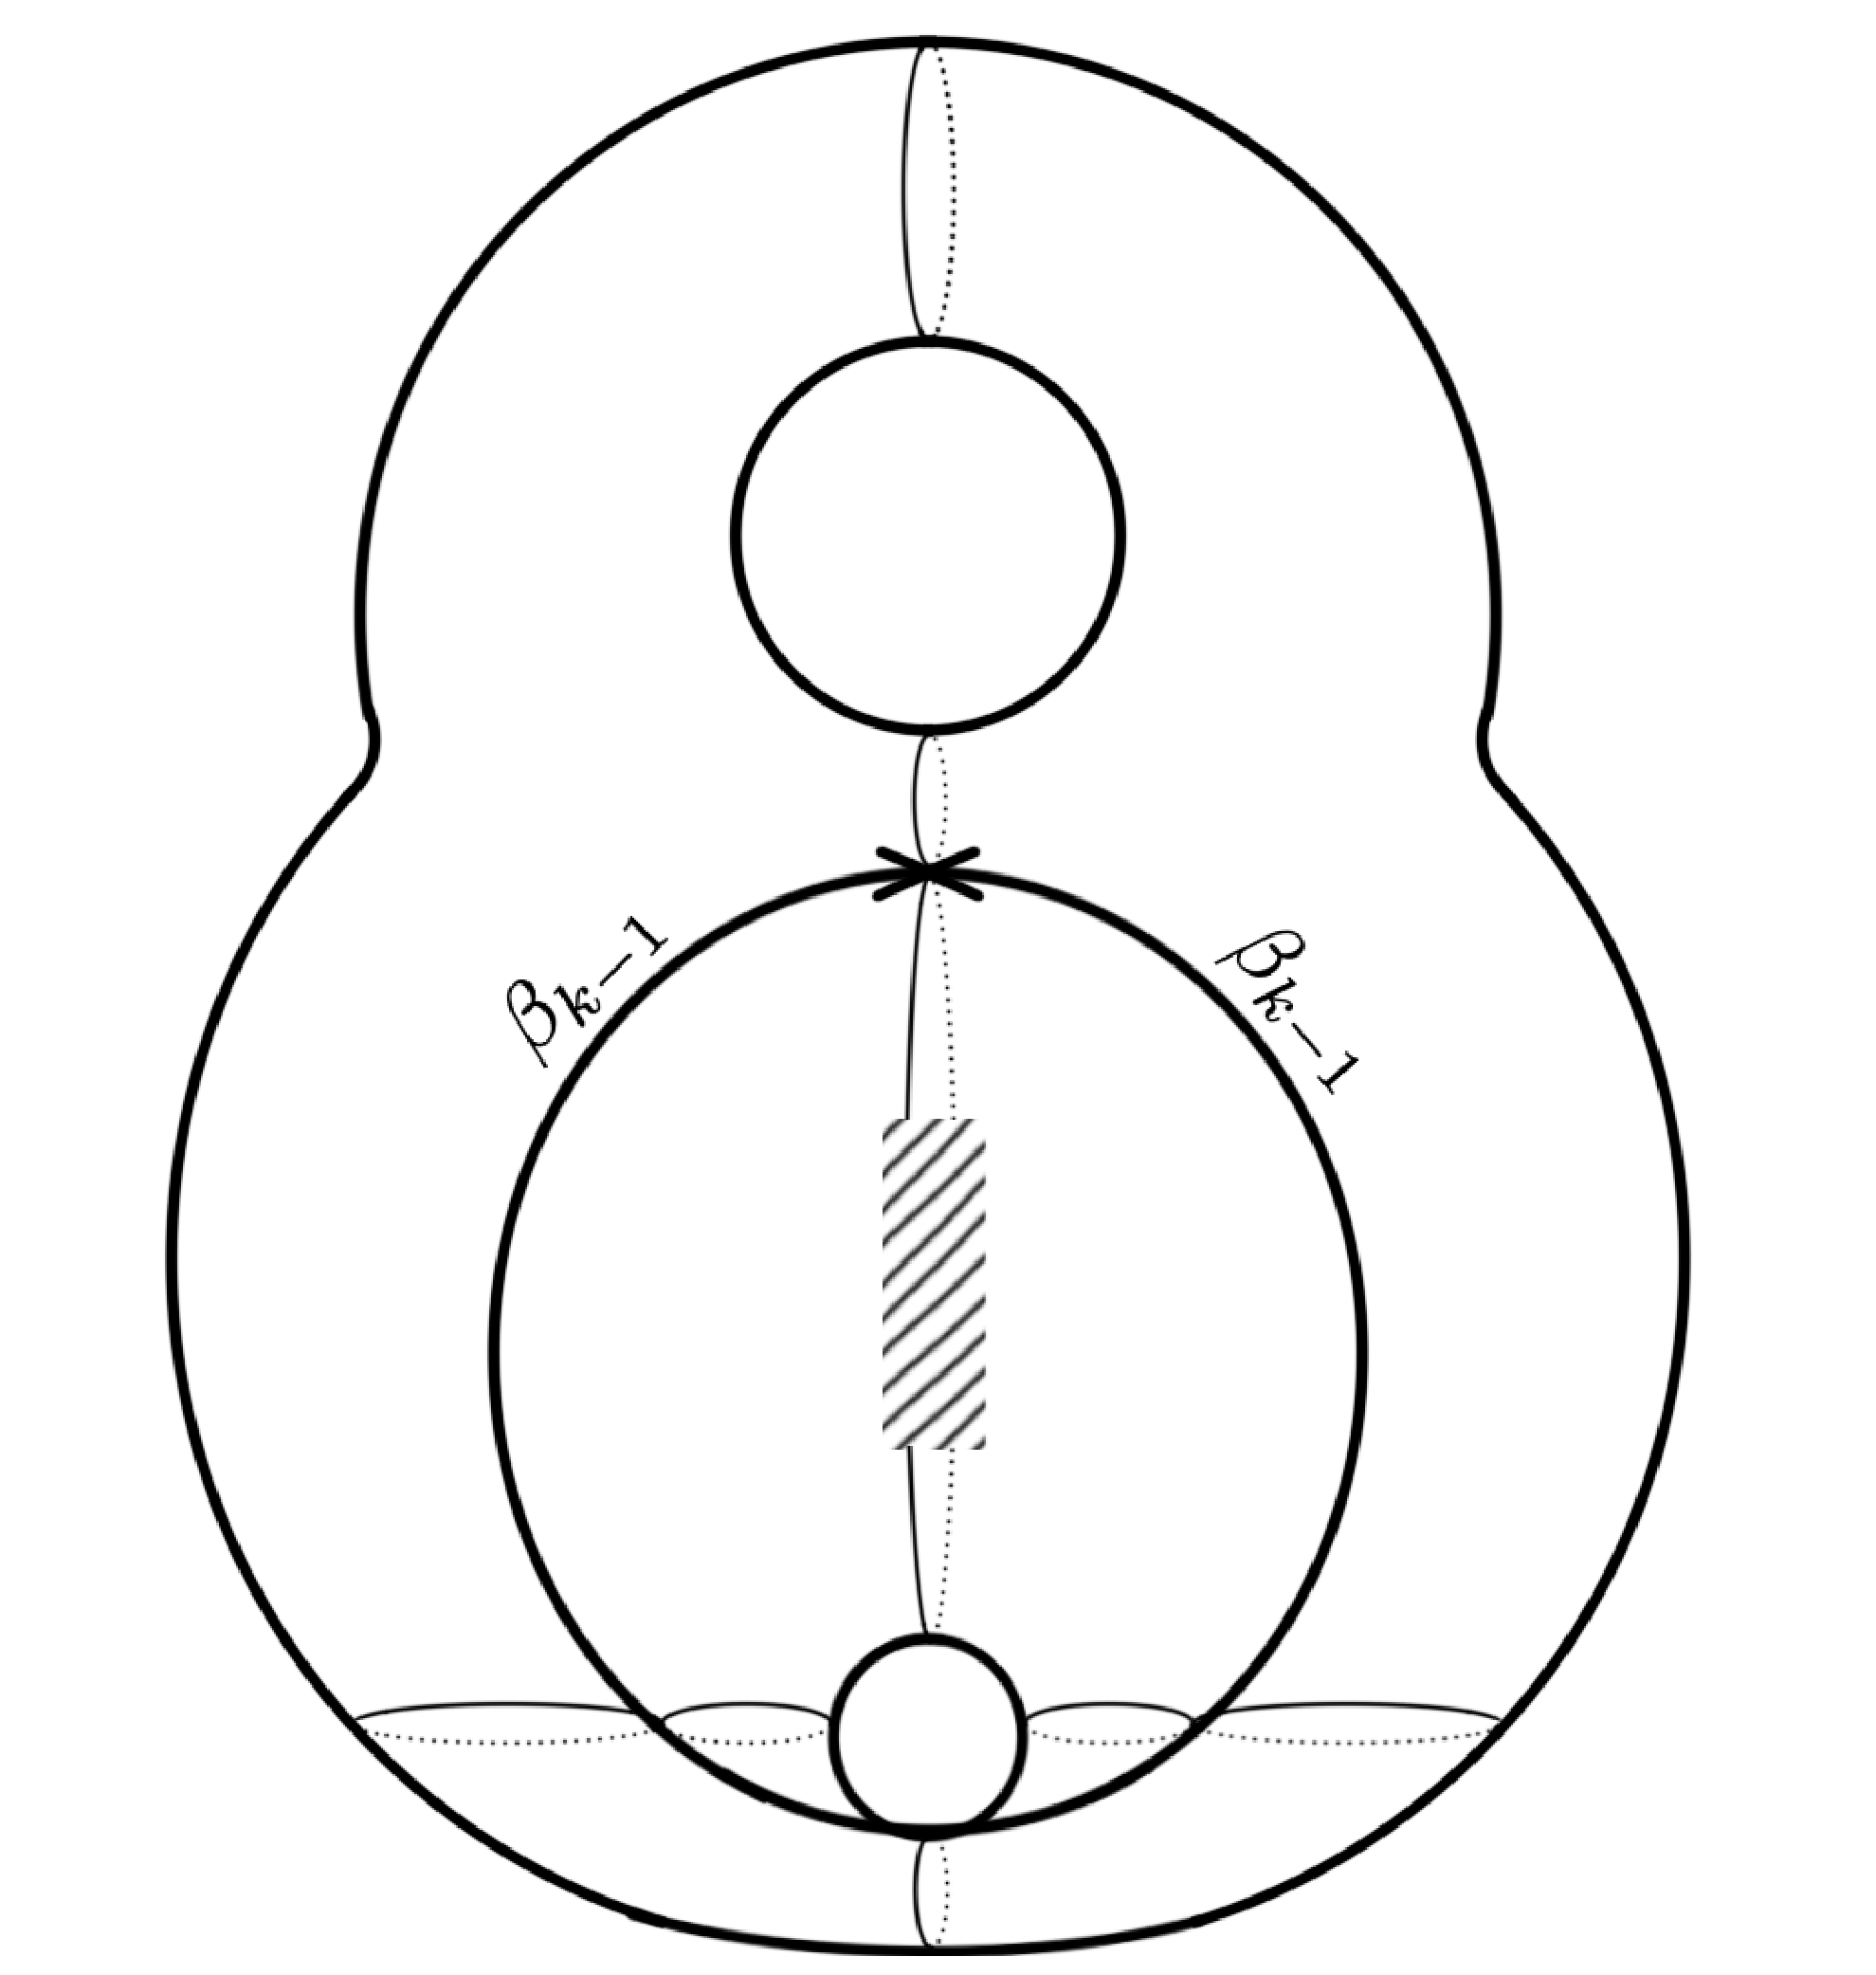
\includegraphics[scale=0.12]{images/ch4/section3_circular/atoms/III/surface.pdf}
    \caption{Особая поверхность.}
        \label{fig:pt10:_III_surface}
\endminipage\hfill
\end{figure}

В точке бифуркации траектории в области $\Omega_2$ направлены по касательным к окружности радиуса $r_1$. Тогда на месте дуги $\beta_{k-1}$ появляется правило отождествления векторов  $c$, определенное в уравнении \eqref{eq:RCrules_circle}. Склеим листы $\widetilde{\Omega}_1$ и $\widetilde{\Omega}_4$ по дугам, проецирующимся на дуги окружностей (то есть по правилам склейки $c$), результат изображен на рис. \ref{fig:pt10:_III_surface_half}. Аналогично для $\widetilde{\Omega}_2$ и $\widetilde{\Omega}_3$. По общим границам склеивая получившиеся поверхности, получим особую поверхность, как изображено на рис. \ref{fig:pt10:_III_surface}. 

После бифуркации склейка на месте $\beta_{k-1}$ исчезает, и две поверхности (обе являются сферами с ручками) перестают быть соединены. При этом, если пересекалась прямая $III_m$ с параметром $m=\left\lfloor \frac{||L_1||}{\gamma} \right\rfloor$, то после бифуркации мы остаемся на <<внешней>> сфере с ручками. При меньших значениях параметра после точки бифуркации поверхность уровня является поверхностью, в которой мы заштриховали вариативную часть.
 \begin{remark}
 Приведенные рассуждения для $\rho_1^2 > r_2^2$ аналогичны, особая поверхность снова будет получаться как отождествление отрезка на сфере с заштрихованными ручками с окружностью на другой поверхности, как на рис. \ref{fig:pt10:_III_surface}. Единственное отличие заключается в том, что при $\rho_1^2 > r_2^2$ в качестве <<внешней>> сферы с ручками выступает тор.
 \end{remark}
 
 \subsection{Семейство $IV$}
Пересечение произвольной кривой $IV_m$ соответствует случаю $\rho_1^2 = r_2^2$. Тогда в области $\Omega_1$ траектории направлены вдоль граничной окружности радиуса $r_2$. Эта бифуркация соответствует особой поверхности, которая получается из \ref{fig:pt10:_terminal_max_domain} переходом к \ref{fig:pt10:_terminal_max_domain_B1Prime} (или переходом из \ref{fig:pt10:_C1_domain} к \ref{fig:pt10:_C1_domainPrime}). Очевидно, что особая поверхность получается как предел неособой, при котором одна из ручек схлопывается в дугу окружности.


\subsection{Случай $n_1^2 > n_2^2$}
Применимы соображения, аналогичные приведенным в \ref{sec:ch5/sec6/sub2}. Следует использовать уравнения для кривых семейств $I, \ldots, III$, приведенные в утверждении \ref{st:curves_formulas}. Сами особые поверхности будут соответствовать пересечениям кривых семейств $II, III, IV$. При этом, как можно заметить из сходств рис. \ref{fig:pt10:_big_domain_transformed} и  рис. \ref{fig:pt10:_big_domain_transformed_2}, особенности будут повторять те, что были  приведены в предыдущем разделе.
